\documentclass[twoside]{book}

% Packages required by doxygen
\usepackage{fixltx2e}
\usepackage{calc}
\usepackage{doxygen}
\usepackage[export]{adjustbox} % also loads graphicx
\usepackage{graphicx}
\usepackage[utf8]{inputenc}
\usepackage{makeidx}
\usepackage{multicol}
\usepackage{multirow}
\PassOptionsToPackage{warn}{textcomp}
\usepackage{textcomp}
\usepackage[nointegrals]{wasysym}
\usepackage[table]{xcolor}

% Font selection
\usepackage[T1]{fontenc}
\usepackage[scaled=.90]{helvet}
\usepackage{courier}
\usepackage{amssymb}
\usepackage{sectsty}
\renewcommand{\familydefault}{\sfdefault}
\allsectionsfont{%
  \fontseries{bc}\selectfont%
  \color{darkgray}%
}
\renewcommand{\DoxyLabelFont}{%
  \fontseries{bc}\selectfont%
  \color{darkgray}%
}
\newcommand{\+}{\discretionary{\mbox{\scriptsize$\hookleftarrow$}}{}{}}

% Page & text layout
\usepackage{geometry}
\geometry{%
  a4paper,%
  top=2.5cm,%
  bottom=2.5cm,%
  left=2.5cm,%
  right=2.5cm%
}
\tolerance=750
\hfuzz=15pt
\hbadness=750
\setlength{\emergencystretch}{15pt}
\setlength{\parindent}{0cm}
\setlength{\parskip}{3ex plus 2ex minus 2ex}
\makeatletter
\renewcommand{\paragraph}{%
  \@startsection{paragraph}{4}{0ex}{-1.0ex}{1.0ex}{%
    \normalfont\normalsize\bfseries\SS@parafont%
  }%
}
\renewcommand{\subparagraph}{%
  \@startsection{subparagraph}{5}{0ex}{-1.0ex}{1.0ex}{%
    \normalfont\normalsize\bfseries\SS@subparafont%
  }%
}
\makeatother

% Headers & footers
\usepackage{fancyhdr}
\pagestyle{fancyplain}
\fancyhead[LE]{\fancyplain{}{\bfseries\thepage}}
\fancyhead[CE]{\fancyplain{}{}}
\fancyhead[RE]{\fancyplain{}{\bfseries\leftmark}}
\fancyhead[LO]{\fancyplain{}{\bfseries\rightmark}}
\fancyhead[CO]{\fancyplain{}{}}
\fancyhead[RO]{\fancyplain{}{\bfseries\thepage}}
\fancyfoot[LE]{\fancyplain{}{}}
\fancyfoot[CE]{\fancyplain{}{}}
\fancyfoot[RE]{\fancyplain{}{\bfseries\scriptsize Generated by Doxygen }}
\fancyfoot[LO]{\fancyplain{}{\bfseries\scriptsize Generated by Doxygen }}
\fancyfoot[CO]{\fancyplain{}{}}
\fancyfoot[RO]{\fancyplain{}{}}
\renewcommand{\footrulewidth}{0.4pt}
\renewcommand{\chaptermark}[1]{%
  \markboth{#1}{}%
}
\renewcommand{\sectionmark}[1]{%
  \markright{\thesection\ #1}%
}

% Indices & bibliography
\usepackage{natbib}
\usepackage[titles]{tocloft}
\setcounter{tocdepth}{3}
\setcounter{secnumdepth}{5}
\makeindex

% Hyperlinks (required, but should be loaded last)
\usepackage{ifpdf}
\ifpdf
  \usepackage[pdftex,pagebackref=true]{hyperref}
\else
  \usepackage[ps2pdf,pagebackref=true]{hyperref}
\fi
\hypersetup{%
  colorlinks=true,%
  linkcolor=blue,%
  citecolor=blue,%
  unicode%
}

% Custom commands
\newcommand{\clearemptydoublepage}{%
  \newpage{\pagestyle{empty}\cleardoublepage}%
}

\usepackage{caption}
\captionsetup{labelsep=space,justification=centering,font={bf},singlelinecheck=off,skip=4pt,position=top}

%===== C O N T E N T S =====

\begin{document}

% Titlepage & ToC
\hypersetup{pageanchor=false,
             bookmarksnumbered=true,
             pdfencoding=unicode
            }
\pagenumbering{roman}
\begin{titlepage}
\vspace*{7cm}
\begin{center}%
{\Large Group Woolly Mammoth }\\
\vspace*{1cm}
{\large Generated by Doxygen 1.8.11}\\
\end{center}
\end{titlepage}
\clearemptydoublepage
\tableofcontents
\clearemptydoublepage
\pagenumbering{arabic}
\hypersetup{pageanchor=true}

%--- Begin generated contents ---
\chapter{Namespace Index}
\section{Namespace List}
Here is a list of all namespaces with brief descriptions\+:\begin{DoxyCompactList}
\item\contentsline{section}{\hyperlink{namespacefcal}{fcal} }{\pageref{namespacefcal}}{}
\item\contentsline{section}{\hyperlink{namespacefcal_1_1ast}{fcal\+::ast} }{\pageref{namespacefcal_1_1ast}}{}
\item\contentsline{section}{\hyperlink{namespacefcal_1_1parser}{fcal\+::parser} }{\pageref{namespacefcal_1_1parser}}{}
\item\contentsline{section}{\hyperlink{namespacefcal_1_1scanner}{fcal\+::scanner} }{\pageref{namespacefcal_1_1scanner}}{}
\end{DoxyCompactList}

\chapter{Hierarchical Index}
\section{Class Hierarchy}
This inheritance list is sorted roughly, but not completely, alphabetically\+:\begin{DoxyCompactList}
\item \contentsline{section}{fcal\+:\+:scanner\+:\+:Ext\+Token}{\pageref{classfcal_1_1scanner_1_1ExtToken}}{}
\begin{DoxyCompactList}
\item \contentsline{section}{fcal\+:\+:scanner\+:\+:Char\+Const\+Token}{\pageref{classfcal_1_1scanner_1_1CharConstToken}}{}
\item \contentsline{section}{fcal\+:\+:scanner\+:\+:Dash\+Token}{\pageref{classfcal_1_1scanner_1_1DashToken}}{}
\item \contentsline{section}{fcal\+:\+:scanner\+:\+:End\+Of\+File\+Token}{\pageref{classfcal_1_1scanner_1_1EndOfFileToken}}{}
\item \contentsline{section}{fcal\+:\+:scanner\+:\+:False\+Kwd\+Token}{\pageref{classfcal_1_1scanner_1_1FalseKwdToken}}{}
\item \contentsline{section}{fcal\+:\+:scanner\+:\+:Float\+Const\+Token}{\pageref{classfcal_1_1scanner_1_1FloatConstToken}}{}
\item \contentsline{section}{fcal\+:\+:scanner\+:\+:Forward\+Slash\+Token}{\pageref{classfcal_1_1scanner_1_1ForwardSlashToken}}{}
\item \contentsline{section}{fcal\+:\+:scanner\+:\+:If\+Token}{\pageref{classfcal_1_1scanner_1_1IfToken}}{}
\item \contentsline{section}{fcal\+:\+:scanner\+:\+:Int\+Const\+Token}{\pageref{classfcal_1_1scanner_1_1IntConstToken}}{}
\item \contentsline{section}{fcal\+:\+:scanner\+:\+:Left\+Paren\+Token}{\pageref{classfcal_1_1scanner_1_1LeftParenToken}}{}
\item \contentsline{section}{fcal\+:\+:scanner\+:\+:Let\+Token}{\pageref{classfcal_1_1scanner_1_1LetToken}}{}
\item \contentsline{section}{fcal\+:\+:scanner\+:\+:Not\+Op\+Token}{\pageref{classfcal_1_1scanner_1_1NotOpToken}}{}
\item \contentsline{section}{fcal\+:\+:scanner\+:\+:Plus\+Sign\+Token}{\pageref{classfcal_1_1scanner_1_1PlusSignToken}}{}
\item \contentsline{section}{fcal\+:\+:scanner\+:\+:Relational\+Op\+Token}{\pageref{classfcal_1_1scanner_1_1RelationalOpToken}}{}
\item \contentsline{section}{fcal\+:\+:scanner\+:\+:Star\+Token}{\pageref{classfcal_1_1scanner_1_1StarToken}}{}
\item \contentsline{section}{fcal\+:\+:scanner\+:\+:String\+Const\+Token}{\pageref{classfcal_1_1scanner_1_1StringConstToken}}{}
\item \contentsline{section}{fcal\+:\+:scanner\+:\+:True\+Kwd\+Token}{\pageref{classfcal_1_1scanner_1_1TrueKwdToken}}{}
\item \contentsline{section}{fcal\+:\+:scanner\+:\+:Variable\+Name\+Token}{\pageref{classfcal_1_1scanner_1_1VariableNameToken}}{}
\end{DoxyCompactList}
\item \contentsline{section}{My\+Sequence$<$ T, N $>$}{\pageref{classMySequence}}{}
\item \contentsline{section}{fcal\+:\+:ast\+:\+:Node}{\pageref{classfcal_1_1ast_1_1Node}}{}
\begin{DoxyCompactList}
\item \contentsline{section}{fcal\+:\+:ast\+:\+:Decl}{\pageref{classfcal_1_1ast_1_1Decl}}{}
\begin{DoxyCompactList}
\item \contentsline{section}{fcal\+:\+:ast\+:\+:Boolean\+Decl}{\pageref{classfcal_1_1ast_1_1BooleanDecl}}{}
\item \contentsline{section}{fcal\+:\+:ast\+:\+:Float\+Decl}{\pageref{classfcal_1_1ast_1_1FloatDecl}}{}
\item \contentsline{section}{fcal\+:\+:ast\+:\+:Int\+Decl}{\pageref{classfcal_1_1ast_1_1IntDecl}}{}
\item \contentsline{section}{fcal\+:\+:ast\+:\+:Matrix\+Multi\+Expr\+Decl}{\pageref{classfcal_1_1ast_1_1MatrixMultiExprDecl}}{}
\item \contentsline{section}{fcal\+:\+:ast\+:\+:Matrix\+Single\+Expr\+Decl}{\pageref{classfcal_1_1ast_1_1MatrixSingleExprDecl}}{}
\item \contentsline{section}{fcal\+:\+:ast\+:\+:String\+Decl}{\pageref{classfcal_1_1ast_1_1StringDecl}}{}
\end{DoxyCompactList}
\item \contentsline{section}{fcal\+:\+:ast\+:\+:Expr}{\pageref{classfcal_1_1ast_1_1Expr}}{}
\begin{DoxyCompactList}
\item \contentsline{section}{fcal\+:\+:ast\+:\+:Add\+Expr}{\pageref{classfcal_1_1ast_1_1AddExpr}}{}
\item \contentsline{section}{fcal\+:\+:ast\+:\+:Boolean\+Const\+Expr}{\pageref{classfcal_1_1ast_1_1BooleanConstExpr}}{}
\item \contentsline{section}{fcal\+:\+:ast\+:\+:Divide\+Expr}{\pageref{classfcal_1_1ast_1_1DivideExpr}}{}
\item \contentsline{section}{fcal\+:\+:ast\+:\+:Equals\+Equals\+Expr}{\pageref{classfcal_1_1ast_1_1EqualsEqualsExpr}}{}
\item \contentsline{section}{fcal\+:\+:ast\+:\+:Float\+Const\+Expr}{\pageref{classfcal_1_1ast_1_1FloatConstExpr}}{}
\item \contentsline{section}{fcal\+:\+:ast\+:\+:Greater\+Equal\+Expr}{\pageref{classfcal_1_1ast_1_1GreaterEqualExpr}}{}
\item \contentsline{section}{fcal\+:\+:ast\+:\+:Greater\+Expr}{\pageref{classfcal_1_1ast_1_1GreaterExpr}}{}
\item \contentsline{section}{fcal\+:\+:ast\+:\+:If\+Expr}{\pageref{classfcal_1_1ast_1_1IfExpr}}{}
\item \contentsline{section}{fcal\+:\+:ast\+:\+:Integer\+Const\+Expr}{\pageref{classfcal_1_1ast_1_1IntegerConstExpr}}{}
\item \contentsline{section}{fcal\+:\+:ast\+:\+:Less\+Equal\+Expr}{\pageref{classfcal_1_1ast_1_1LessEqualExpr}}{}
\item \contentsline{section}{fcal\+:\+:ast\+:\+:Less\+Expr}{\pageref{classfcal_1_1ast_1_1LessExpr}}{}
\item \contentsline{section}{fcal\+:\+:ast\+:\+:Let\+Expr}{\pageref{classfcal_1_1ast_1_1LetExpr}}{}
\item \contentsline{section}{fcal\+:\+:ast\+:\+:Logical\+And\+Expr}{\pageref{classfcal_1_1ast_1_1LogicalAndExpr}}{}
\item \contentsline{section}{fcal\+:\+:ast\+:\+:Logical\+Or\+Expr}{\pageref{classfcal_1_1ast_1_1LogicalOrExpr}}{}
\item \contentsline{section}{fcal\+:\+:ast\+:\+:Matrix\+R\+E\+F\+Expr}{\pageref{classfcal_1_1ast_1_1MatrixREFExpr}}{}
\item \contentsline{section}{fcal\+:\+:ast\+:\+:Multiply\+Expr}{\pageref{classfcal_1_1ast_1_1MultiplyExpr}}{}
\item \contentsline{section}{fcal\+:\+:ast\+:\+:Nested\+Or\+Function\+Call\+Expr}{\pageref{classfcal_1_1ast_1_1NestedOrFunctionCallExpr}}{}
\item \contentsline{section}{fcal\+:\+:ast\+:\+:Not\+Equals\+Expr}{\pageref{classfcal_1_1ast_1_1NotEqualsExpr}}{}
\item \contentsline{section}{fcal\+:\+:ast\+:\+:Not\+Expr}{\pageref{classfcal_1_1ast_1_1NotExpr}}{}
\item \contentsline{section}{fcal\+:\+:ast\+:\+:Parentheses\+Expr}{\pageref{classfcal_1_1ast_1_1ParenthesesExpr}}{}
\item \contentsline{section}{fcal\+:\+:ast\+:\+:String\+Const\+Expr}{\pageref{classfcal_1_1ast_1_1StringConstExpr}}{}
\item \contentsline{section}{fcal\+:\+:ast\+:\+:Subtract\+Expr}{\pageref{classfcal_1_1ast_1_1SubtractExpr}}{}
\item \contentsline{section}{fcal\+:\+:ast\+:\+:Var\+Name\+Expr}{\pageref{classfcal_1_1ast_1_1VarNameExpr}}{}
\end{DoxyCompactList}
\item \contentsline{section}{fcal\+:\+:ast\+:\+:Program}{\pageref{classfcal_1_1ast_1_1Program}}{}
\item \contentsline{section}{fcal\+:\+:ast\+:\+:Stmt}{\pageref{classfcal_1_1ast_1_1Stmt}}{}
\begin{DoxyCompactList}
\item \contentsline{section}{fcal\+:\+:ast\+:\+:Assign\+Stmt}{\pageref{classfcal_1_1ast_1_1AssignStmt}}{}
\item \contentsline{section}{fcal\+:\+:ast\+:\+:Brackets\+Stmt}{\pageref{classfcal_1_1ast_1_1BracketsStmt}}{}
\item \contentsline{section}{fcal\+:\+:ast\+:\+:Decl\+Stmt}{\pageref{classfcal_1_1ast_1_1DeclStmt}}{}
\item \contentsline{section}{fcal\+:\+:ast\+:\+:If\+Else\+Stmt}{\pageref{classfcal_1_1ast_1_1IfElseStmt}}{}
\item \contentsline{section}{fcal\+:\+:ast\+:\+:If\+Stmt}{\pageref{classfcal_1_1ast_1_1IfStmt}}{}
\item \contentsline{section}{fcal\+:\+:ast\+:\+:Matrix\+Assign\+Stmt}{\pageref{classfcal_1_1ast_1_1MatrixAssignStmt}}{}
\item \contentsline{section}{fcal\+:\+:ast\+:\+:Print\+Stmt}{\pageref{classfcal_1_1ast_1_1PrintStmt}}{}
\item \contentsline{section}{fcal\+:\+:ast\+:\+:Repeat\+Stmt}{\pageref{classfcal_1_1ast_1_1RepeatStmt}}{}
\item \contentsline{section}{fcal\+:\+:ast\+:\+:Semi\+Colon\+Stmt}{\pageref{classfcal_1_1ast_1_1SemiColonStmt}}{}
\item \contentsline{section}{fcal\+:\+:ast\+:\+:While\+Stmt}{\pageref{classfcal_1_1ast_1_1WhileStmt}}{}
\end{DoxyCompactList}
\item \contentsline{section}{fcal\+:\+:ast\+:\+:Stmts}{\pageref{classfcal_1_1ast_1_1Stmts}}{}
\begin{DoxyCompactList}
\item \contentsline{section}{fcal\+:\+:ast\+:\+:Empty\+Stmts}{\pageref{classfcal_1_1ast_1_1EmptyStmts}}{}
\item \contentsline{section}{fcal\+:\+:ast\+:\+:Seq\+Stmts}{\pageref{classfcal_1_1ast_1_1SeqStmts}}{}
\end{DoxyCompactList}
\end{DoxyCompactList}
\item \contentsline{section}{fcal\+:\+:parser\+:\+:Parser}{\pageref{classfcal_1_1parser_1_1Parser}}{}
\item \contentsline{section}{fcal\+:\+:parser\+:\+:Parse\+Result}{\pageref{classfcal_1_1parser_1_1ParseResult}}{}
\item \contentsline{section}{fcal\+:\+:scanner\+:\+:Scanner}{\pageref{classfcal_1_1scanner_1_1Scanner}}{}
\item \contentsline{section}{fcal\+:\+:scanner\+:\+:Token}{\pageref{classfcal_1_1scanner_1_1Token}}{}
\end{DoxyCompactList}

\chapter{Class Index}
\section{Class List}
Here are the classes, structs, unions and interfaces with brief descriptions\+:\begin{DoxyCompactList}
\item\contentsline{section}{\hyperlink{classfcal_1_1ast_1_1AddExpr}{fcal\+::ast\+::\+Add\+Expr} }{\pageref{classfcal_1_1ast_1_1AddExpr}}{}
\item\contentsline{section}{\hyperlink{classfcal_1_1ast_1_1AssignStmt}{fcal\+::ast\+::\+Assign\+Stmt} }{\pageref{classfcal_1_1ast_1_1AssignStmt}}{}
\item\contentsline{section}{\hyperlink{classfcal_1_1ast_1_1BooleanConstExpr}{fcal\+::ast\+::\+Boolean\+Const\+Expr} }{\pageref{classfcal_1_1ast_1_1BooleanConstExpr}}{}
\item\contentsline{section}{\hyperlink{classfcal_1_1ast_1_1BooleanDecl}{fcal\+::ast\+::\+Boolean\+Decl} }{\pageref{classfcal_1_1ast_1_1BooleanDecl}}{}
\item\contentsline{section}{\hyperlink{classfcal_1_1ast_1_1BracketsStmt}{fcal\+::ast\+::\+Brackets\+Stmt} }{\pageref{classfcal_1_1ast_1_1BracketsStmt}}{}
\item\contentsline{section}{\hyperlink{classfcal_1_1scanner_1_1CharConstToken}{fcal\+::scanner\+::\+Char\+Const\+Token} }{\pageref{classfcal_1_1scanner_1_1CharConstToken}}{}
\item\contentsline{section}{\hyperlink{classfcal_1_1scanner_1_1DashToken}{fcal\+::scanner\+::\+Dash\+Token} }{\pageref{classfcal_1_1scanner_1_1DashToken}}{}
\item\contentsline{section}{\hyperlink{classfcal_1_1ast_1_1Decl}{fcal\+::ast\+::\+Decl} }{\pageref{classfcal_1_1ast_1_1Decl}}{}
\item\contentsline{section}{\hyperlink{classfcal_1_1ast_1_1DeclStmt}{fcal\+::ast\+::\+Decl\+Stmt} }{\pageref{classfcal_1_1ast_1_1DeclStmt}}{}
\item\contentsline{section}{\hyperlink{classfcal_1_1ast_1_1DivideExpr}{fcal\+::ast\+::\+Divide\+Expr} }{\pageref{classfcal_1_1ast_1_1DivideExpr}}{}
\item\contentsline{section}{\hyperlink{classfcal_1_1ast_1_1EmptyStmts}{fcal\+::ast\+::\+Empty\+Stmts} }{\pageref{classfcal_1_1ast_1_1EmptyStmts}}{}
\item\contentsline{section}{\hyperlink{classfcal_1_1scanner_1_1EndOfFileToken}{fcal\+::scanner\+::\+End\+Of\+File\+Token} }{\pageref{classfcal_1_1scanner_1_1EndOfFileToken}}{}
\item\contentsline{section}{\hyperlink{classfcal_1_1ast_1_1EqualsEqualsExpr}{fcal\+::ast\+::\+Equals\+Equals\+Expr} }{\pageref{classfcal_1_1ast_1_1EqualsEqualsExpr}}{}
\item\contentsline{section}{\hyperlink{classfcal_1_1ast_1_1Expr}{fcal\+::ast\+::\+Expr} }{\pageref{classfcal_1_1ast_1_1Expr}}{}
\item\contentsline{section}{\hyperlink{classfcal_1_1scanner_1_1ExtToken}{fcal\+::scanner\+::\+Ext\+Token} }{\pageref{classfcal_1_1scanner_1_1ExtToken}}{}
\item\contentsline{section}{\hyperlink{classfcal_1_1scanner_1_1FalseKwdToken}{fcal\+::scanner\+::\+False\+Kwd\+Token} }{\pageref{classfcal_1_1scanner_1_1FalseKwdToken}}{}
\item\contentsline{section}{\hyperlink{classfcal_1_1ast_1_1FloatConstExpr}{fcal\+::ast\+::\+Float\+Const\+Expr} }{\pageref{classfcal_1_1ast_1_1FloatConstExpr}}{}
\item\contentsline{section}{\hyperlink{classfcal_1_1scanner_1_1FloatConstToken}{fcal\+::scanner\+::\+Float\+Const\+Token} }{\pageref{classfcal_1_1scanner_1_1FloatConstToken}}{}
\item\contentsline{section}{\hyperlink{classfcal_1_1ast_1_1FloatDecl}{fcal\+::ast\+::\+Float\+Decl} }{\pageref{classfcal_1_1ast_1_1FloatDecl}}{}
\item\contentsline{section}{\hyperlink{classfcal_1_1scanner_1_1ForwardSlashToken}{fcal\+::scanner\+::\+Forward\+Slash\+Token} }{\pageref{classfcal_1_1scanner_1_1ForwardSlashToken}}{}
\item\contentsline{section}{\hyperlink{classfcal_1_1ast_1_1GreaterEqualExpr}{fcal\+::ast\+::\+Greater\+Equal\+Expr} }{\pageref{classfcal_1_1ast_1_1GreaterEqualExpr}}{}
\item\contentsline{section}{\hyperlink{classfcal_1_1ast_1_1GreaterExpr}{fcal\+::ast\+::\+Greater\+Expr} }{\pageref{classfcal_1_1ast_1_1GreaterExpr}}{}
\item\contentsline{section}{\hyperlink{classfcal_1_1ast_1_1IfElseStmt}{fcal\+::ast\+::\+If\+Else\+Stmt} }{\pageref{classfcal_1_1ast_1_1IfElseStmt}}{}
\item\contentsline{section}{\hyperlink{classfcal_1_1ast_1_1IfExpr}{fcal\+::ast\+::\+If\+Expr} }{\pageref{classfcal_1_1ast_1_1IfExpr}}{}
\item\contentsline{section}{\hyperlink{classfcal_1_1ast_1_1IfStmt}{fcal\+::ast\+::\+If\+Stmt} }{\pageref{classfcal_1_1ast_1_1IfStmt}}{}
\item\contentsline{section}{\hyperlink{classfcal_1_1scanner_1_1IfToken}{fcal\+::scanner\+::\+If\+Token} }{\pageref{classfcal_1_1scanner_1_1IfToken}}{}
\item\contentsline{section}{\hyperlink{classfcal_1_1scanner_1_1IntConstToken}{fcal\+::scanner\+::\+Int\+Const\+Token} }{\pageref{classfcal_1_1scanner_1_1IntConstToken}}{}
\item\contentsline{section}{\hyperlink{classfcal_1_1ast_1_1IntDecl}{fcal\+::ast\+::\+Int\+Decl} }{\pageref{classfcal_1_1ast_1_1IntDecl}}{}
\item\contentsline{section}{\hyperlink{classfcal_1_1ast_1_1IntegerConstExpr}{fcal\+::ast\+::\+Integer\+Const\+Expr} }{\pageref{classfcal_1_1ast_1_1IntegerConstExpr}}{}
\item\contentsline{section}{\hyperlink{classfcal_1_1scanner_1_1LeftParenToken}{fcal\+::scanner\+::\+Left\+Paren\+Token} }{\pageref{classfcal_1_1scanner_1_1LeftParenToken}}{}
\item\contentsline{section}{\hyperlink{classfcal_1_1ast_1_1LessEqualExpr}{fcal\+::ast\+::\+Less\+Equal\+Expr} }{\pageref{classfcal_1_1ast_1_1LessEqualExpr}}{}
\item\contentsline{section}{\hyperlink{classfcal_1_1ast_1_1LessExpr}{fcal\+::ast\+::\+Less\+Expr} }{\pageref{classfcal_1_1ast_1_1LessExpr}}{}
\item\contentsline{section}{\hyperlink{classfcal_1_1ast_1_1LetExpr}{fcal\+::ast\+::\+Let\+Expr} }{\pageref{classfcal_1_1ast_1_1LetExpr}}{}
\item\contentsline{section}{\hyperlink{classfcal_1_1scanner_1_1LetToken}{fcal\+::scanner\+::\+Let\+Token} }{\pageref{classfcal_1_1scanner_1_1LetToken}}{}
\item\contentsline{section}{\hyperlink{classfcal_1_1ast_1_1LogicalAndExpr}{fcal\+::ast\+::\+Logical\+And\+Expr} }{\pageref{classfcal_1_1ast_1_1LogicalAndExpr}}{}
\item\contentsline{section}{\hyperlink{classfcal_1_1ast_1_1LogicalOrExpr}{fcal\+::ast\+::\+Logical\+Or\+Expr} }{\pageref{classfcal_1_1ast_1_1LogicalOrExpr}}{}
\item\contentsline{section}{\hyperlink{classfcal_1_1ast_1_1MatrixAssignStmt}{fcal\+::ast\+::\+Matrix\+Assign\+Stmt} }{\pageref{classfcal_1_1ast_1_1MatrixAssignStmt}}{}
\item\contentsline{section}{\hyperlink{classfcal_1_1ast_1_1MatrixMultiExprDecl}{fcal\+::ast\+::\+Matrix\+Multi\+Expr\+Decl} }{\pageref{classfcal_1_1ast_1_1MatrixMultiExprDecl}}{}
\item\contentsline{section}{\hyperlink{classfcal_1_1ast_1_1MatrixREFExpr}{fcal\+::ast\+::\+Matrix\+R\+E\+F\+Expr} }{\pageref{classfcal_1_1ast_1_1MatrixREFExpr}}{}
\item\contentsline{section}{\hyperlink{classfcal_1_1ast_1_1MatrixSingleExprDecl}{fcal\+::ast\+::\+Matrix\+Single\+Expr\+Decl} }{\pageref{classfcal_1_1ast_1_1MatrixSingleExprDecl}}{}
\item\contentsline{section}{\hyperlink{classfcal_1_1ast_1_1MultiplyExpr}{fcal\+::ast\+::\+Multiply\+Expr} }{\pageref{classfcal_1_1ast_1_1MultiplyExpr}}{}
\item\contentsline{section}{\hyperlink{classMySequence}{My\+Sequence$<$ T, N $>$} }{\pageref{classMySequence}}{}
\item\contentsline{section}{\hyperlink{classfcal_1_1ast_1_1NestedOrFunctionCallExpr}{fcal\+::ast\+::\+Nested\+Or\+Function\+Call\+Expr} }{\pageref{classfcal_1_1ast_1_1NestedOrFunctionCallExpr}}{}
\item\contentsline{section}{\hyperlink{classfcal_1_1ast_1_1Node}{fcal\+::ast\+::\+Node} }{\pageref{classfcal_1_1ast_1_1Node}}{}
\item\contentsline{section}{\hyperlink{classfcal_1_1ast_1_1NotEqualsExpr}{fcal\+::ast\+::\+Not\+Equals\+Expr} }{\pageref{classfcal_1_1ast_1_1NotEqualsExpr}}{}
\item\contentsline{section}{\hyperlink{classfcal_1_1ast_1_1NotExpr}{fcal\+::ast\+::\+Not\+Expr} }{\pageref{classfcal_1_1ast_1_1NotExpr}}{}
\item\contentsline{section}{\hyperlink{classfcal_1_1scanner_1_1NotOpToken}{fcal\+::scanner\+::\+Not\+Op\+Token} }{\pageref{classfcal_1_1scanner_1_1NotOpToken}}{}
\item\contentsline{section}{\hyperlink{classfcal_1_1ast_1_1ParenthesesExpr}{fcal\+::ast\+::\+Parentheses\+Expr} }{\pageref{classfcal_1_1ast_1_1ParenthesesExpr}}{}
\item\contentsline{section}{\hyperlink{classfcal_1_1parser_1_1Parser}{fcal\+::parser\+::\+Parser} }{\pageref{classfcal_1_1parser_1_1Parser}}{}
\item\contentsline{section}{\hyperlink{classfcal_1_1parser_1_1ParseResult}{fcal\+::parser\+::\+Parse\+Result} }{\pageref{classfcal_1_1parser_1_1ParseResult}}{}
\item\contentsline{section}{\hyperlink{classfcal_1_1scanner_1_1PlusSignToken}{fcal\+::scanner\+::\+Plus\+Sign\+Token} }{\pageref{classfcal_1_1scanner_1_1PlusSignToken}}{}
\item\contentsline{section}{\hyperlink{classfcal_1_1ast_1_1PrintStmt}{fcal\+::ast\+::\+Print\+Stmt} }{\pageref{classfcal_1_1ast_1_1PrintStmt}}{}
\item\contentsline{section}{\hyperlink{classfcal_1_1ast_1_1Program}{fcal\+::ast\+::\+Program} }{\pageref{classfcal_1_1ast_1_1Program}}{}
\item\contentsline{section}{\hyperlink{classfcal_1_1scanner_1_1RelationalOpToken}{fcal\+::scanner\+::\+Relational\+Op\+Token} }{\pageref{classfcal_1_1scanner_1_1RelationalOpToken}}{}
\item\contentsline{section}{\hyperlink{classfcal_1_1ast_1_1RepeatStmt}{fcal\+::ast\+::\+Repeat\+Stmt} }{\pageref{classfcal_1_1ast_1_1RepeatStmt}}{}
\item\contentsline{section}{\hyperlink{classfcal_1_1scanner_1_1Scanner}{fcal\+::scanner\+::\+Scanner} }{\pageref{classfcal_1_1scanner_1_1Scanner}}{}
\item\contentsline{section}{\hyperlink{classfcal_1_1ast_1_1SemiColonStmt}{fcal\+::ast\+::\+Semi\+Colon\+Stmt} }{\pageref{classfcal_1_1ast_1_1SemiColonStmt}}{}
\item\contentsline{section}{\hyperlink{classfcal_1_1ast_1_1SeqStmts}{fcal\+::ast\+::\+Seq\+Stmts} }{\pageref{classfcal_1_1ast_1_1SeqStmts}}{}
\item\contentsline{section}{\hyperlink{classfcal_1_1scanner_1_1StarToken}{fcal\+::scanner\+::\+Star\+Token} }{\pageref{classfcal_1_1scanner_1_1StarToken}}{}
\item\contentsline{section}{\hyperlink{classfcal_1_1ast_1_1Stmt}{fcal\+::ast\+::\+Stmt} }{\pageref{classfcal_1_1ast_1_1Stmt}}{}
\item\contentsline{section}{\hyperlink{classfcal_1_1ast_1_1Stmts}{fcal\+::ast\+::\+Stmts} }{\pageref{classfcal_1_1ast_1_1Stmts}}{}
\item\contentsline{section}{\hyperlink{classfcal_1_1ast_1_1StringConstExpr}{fcal\+::ast\+::\+String\+Const\+Expr} }{\pageref{classfcal_1_1ast_1_1StringConstExpr}}{}
\item\contentsline{section}{\hyperlink{classfcal_1_1scanner_1_1StringConstToken}{fcal\+::scanner\+::\+String\+Const\+Token} }{\pageref{classfcal_1_1scanner_1_1StringConstToken}}{}
\item\contentsline{section}{\hyperlink{classfcal_1_1ast_1_1StringDecl}{fcal\+::ast\+::\+String\+Decl} }{\pageref{classfcal_1_1ast_1_1StringDecl}}{}
\item\contentsline{section}{\hyperlink{classfcal_1_1ast_1_1SubtractExpr}{fcal\+::ast\+::\+Subtract\+Expr} }{\pageref{classfcal_1_1ast_1_1SubtractExpr}}{}
\item\contentsline{section}{\hyperlink{classfcal_1_1scanner_1_1Token}{fcal\+::scanner\+::\+Token} }{\pageref{classfcal_1_1scanner_1_1Token}}{}
\item\contentsline{section}{\hyperlink{classfcal_1_1scanner_1_1TrueKwdToken}{fcal\+::scanner\+::\+True\+Kwd\+Token} }{\pageref{classfcal_1_1scanner_1_1TrueKwdToken}}{}
\item\contentsline{section}{\hyperlink{classfcal_1_1scanner_1_1VariableNameToken}{fcal\+::scanner\+::\+Variable\+Name\+Token} }{\pageref{classfcal_1_1scanner_1_1VariableNameToken}}{}
\item\contentsline{section}{\hyperlink{classfcal_1_1ast_1_1VarNameExpr}{fcal\+::ast\+::\+Var\+Name\+Expr} }{\pageref{classfcal_1_1ast_1_1VarNameExpr}}{}
\item\contentsline{section}{\hyperlink{classfcal_1_1ast_1_1WhileStmt}{fcal\+::ast\+::\+While\+Stmt} }{\pageref{classfcal_1_1ast_1_1WhileStmt}}{}
\end{DoxyCompactList}

\chapter{File Index}
\section{File List}
Here is a list of all files with brief descriptions\+:\begin{DoxyCompactList}
\item\contentsline{section}{include/\hyperlink{ast_8h}{ast.\+h} }{\pageref{ast_8h}}{}
\item\contentsline{section}{include/\hyperlink{ext__token_8h}{ext\+\_\+token.\+h} }{\pageref{ext__token_8h}}{}
\item\contentsline{section}{include/\hyperlink{iter2scanner_8h}{iter2scanner.\+h} }{\pageref{iter2scanner_8h}}{}
\item\contentsline{section}{include/\hyperlink{parse__result_8h}{parse\+\_\+result.\+h} }{\pageref{parse__result_8h}}{}
\item\contentsline{section}{include/\hyperlink{parser_8h}{parser.\+h} }{\pageref{parser_8h}}{}
\item\contentsline{section}{include/\hyperlink{read__input_8h}{read\+\_\+input.\+h} }{\pageref{read__input_8h}}{}
\item\contentsline{section}{include/\hyperlink{regex_8h}{regex.\+h} }{\pageref{regex_8h}}{}
\item\contentsline{section}{include/\hyperlink{scanner_8h}{scanner.\+h} }{\pageref{scanner_8h}}{}
\item\contentsline{section}{src/\hyperlink{ext__token_8cc}{ext\+\_\+token.\+cc} }{\pageref{ext__token_8cc}}{}
\item\contentsline{section}{src/\hyperlink{parser_8cc}{parser.\+cc} }{\pageref{parser_8cc}}{}
\item\contentsline{section}{src/\hyperlink{read__input_8cc}{read\+\_\+input.\+cc} }{\pageref{read__input_8cc}}{}
\item\contentsline{section}{src/\hyperlink{regex_8cc}{regex.\+cc} }{\pageref{regex_8cc}}{}
\item\contentsline{section}{src/\hyperlink{scanner_8cc}{scanner.\+cc} }{\pageref{scanner_8cc}}{}
\item\contentsline{section}{src/\hyperlink{templates_8cc}{templates.\+cc} }{\pageref{templates_8cc}}{}
\end{DoxyCompactList}

\chapter{Namespace Documentation}
\hypertarget{namespacefcal}{}\section{fcal Namespace Reference}
\label{namespacefcal}\index{fcal@{fcal}}
\subsection*{Namespaces}
\begin{DoxyCompactItemize}
\item 
 \hyperlink{namespacefcal_1_1ast}{ast}
\item 
 \hyperlink{namespacefcal_1_1parser}{parser}
\item 
 \hyperlink{namespacefcal_1_1scanner}{scanner}
\end{DoxyCompactItemize}

\hypertarget{namespacefcal_1_1ast}{}\section{fcal\+:\+:ast Namespace Reference}
\label{namespacefcal_1_1ast}\index{fcal\+::ast@{fcal\+::ast}}
\subsection*{Classes}
\begin{DoxyCompactItemize}
\item 
class \hyperlink{classfcal_1_1ast_1_1AddExpr}{Add\+Expr}
\item 
class \hyperlink{classfcal_1_1ast_1_1AssignStmt}{Assign\+Stmt}
\item 
class \hyperlink{classfcal_1_1ast_1_1BooleanConstExpr}{Boolean\+Const\+Expr}
\item 
class \hyperlink{classfcal_1_1ast_1_1BooleanDecl}{Boolean\+Decl}
\item 
class \hyperlink{classfcal_1_1ast_1_1BracketsStmt}{Brackets\+Stmt}
\item 
class \hyperlink{classfcal_1_1ast_1_1Decl}{Decl}
\item 
class \hyperlink{classfcal_1_1ast_1_1DeclStmt}{Decl\+Stmt}
\item 
class \hyperlink{classfcal_1_1ast_1_1DivideExpr}{Divide\+Expr}
\item 
class \hyperlink{classfcal_1_1ast_1_1EmptyStmts}{Empty\+Stmts}
\item 
class \hyperlink{classfcal_1_1ast_1_1EqualsEqualsExpr}{Equals\+Equals\+Expr}
\item 
class \hyperlink{classfcal_1_1ast_1_1Expr}{Expr}
\item 
class \hyperlink{classfcal_1_1ast_1_1FloatConstExpr}{Float\+Const\+Expr}
\item 
class \hyperlink{classfcal_1_1ast_1_1FloatDecl}{Float\+Decl}
\item 
class \hyperlink{classfcal_1_1ast_1_1GreaterEqualExpr}{Greater\+Equal\+Expr}
\item 
class \hyperlink{classfcal_1_1ast_1_1GreaterExpr}{Greater\+Expr}
\item 
class \hyperlink{classfcal_1_1ast_1_1IfElseStmt}{If\+Else\+Stmt}
\item 
class \hyperlink{classfcal_1_1ast_1_1IfExpr}{If\+Expr}
\item 
class \hyperlink{classfcal_1_1ast_1_1IfStmt}{If\+Stmt}
\item 
class \hyperlink{classfcal_1_1ast_1_1IntDecl}{Int\+Decl}
\item 
class \hyperlink{classfcal_1_1ast_1_1IntegerConstExpr}{Integer\+Const\+Expr}
\item 
class \hyperlink{classfcal_1_1ast_1_1LessEqualExpr}{Less\+Equal\+Expr}
\item 
class \hyperlink{classfcal_1_1ast_1_1LessExpr}{Less\+Expr}
\item 
class \hyperlink{classfcal_1_1ast_1_1LetExpr}{Let\+Expr}
\item 
class \hyperlink{classfcal_1_1ast_1_1LogicalAndExpr}{Logical\+And\+Expr}
\item 
class \hyperlink{classfcal_1_1ast_1_1LogicalOrExpr}{Logical\+Or\+Expr}
\item 
class \hyperlink{classfcal_1_1ast_1_1MatrixAssignStmt}{Matrix\+Assign\+Stmt}
\item 
class \hyperlink{classfcal_1_1ast_1_1MatrixMultiExprDecl}{Matrix\+Multi\+Expr\+Decl}
\item 
class \hyperlink{classfcal_1_1ast_1_1MatrixREFExpr}{Matrix\+R\+E\+F\+Expr}
\item 
class \hyperlink{classfcal_1_1ast_1_1MatrixSingleExprDecl}{Matrix\+Single\+Expr\+Decl}
\item 
class \hyperlink{classfcal_1_1ast_1_1MultiplyExpr}{Multiply\+Expr}
\item 
class \hyperlink{classfcal_1_1ast_1_1NestedOrFunctionCallExpr}{Nested\+Or\+Function\+Call\+Expr}
\item 
class \hyperlink{classfcal_1_1ast_1_1Node}{Node}
\item 
class \hyperlink{classfcal_1_1ast_1_1NotEqualsExpr}{Not\+Equals\+Expr}
\item 
class \hyperlink{classfcal_1_1ast_1_1NotExpr}{Not\+Expr}
\item 
class \hyperlink{classfcal_1_1ast_1_1ParenthesesExpr}{Parentheses\+Expr}
\item 
class \hyperlink{classfcal_1_1ast_1_1PrintStmt}{Print\+Stmt}
\item 
class \hyperlink{classfcal_1_1ast_1_1Program}{Program}
\item 
class \hyperlink{classfcal_1_1ast_1_1RepeatStmt}{Repeat\+Stmt}
\item 
class \hyperlink{classfcal_1_1ast_1_1SemiColonStmt}{Semi\+Colon\+Stmt}
\item 
class \hyperlink{classfcal_1_1ast_1_1SeqStmts}{Seq\+Stmts}
\item 
class \hyperlink{classfcal_1_1ast_1_1Stmt}{Stmt}
\item 
class \hyperlink{classfcal_1_1ast_1_1Stmts}{Stmts}
\item 
class \hyperlink{classfcal_1_1ast_1_1StringConstExpr}{String\+Const\+Expr}
\item 
class \hyperlink{classfcal_1_1ast_1_1StringDecl}{String\+Decl}
\item 
class \hyperlink{classfcal_1_1ast_1_1SubtractExpr}{Subtract\+Expr}
\item 
class \hyperlink{classfcal_1_1ast_1_1VarNameExpr}{Var\+Name\+Expr}
\item 
class \hyperlink{classfcal_1_1ast_1_1WhileStmt}{While\+Stmt}
\end{DoxyCompactItemize}

\hypertarget{namespacefcal_1_1parser}{}\section{fcal\+:\+:parser Namespace Reference}
\label{namespacefcal_1_1parser}\index{fcal\+::parser@{fcal\+::parser}}
\subsection*{Classes}
\begin{DoxyCompactItemize}
\item 
class \hyperlink{classfcal_1_1parser_1_1Parser}{Parser}
\item 
class \hyperlink{classfcal_1_1parser_1_1ParseResult}{Parse\+Result}
\end{DoxyCompactItemize}

\hypertarget{namespacefcal_1_1scanner}{}\section{fcal\+:\+:scanner Namespace Reference}
\label{namespacefcal_1_1scanner}\index{fcal\+::scanner@{fcal\+::scanner}}
\subsection*{Classes}
\begin{DoxyCompactItemize}
\item 
class \hyperlink{classfcal_1_1scanner_1_1CharConstToken}{Char\+Const\+Token}
\item 
class \hyperlink{classfcal_1_1scanner_1_1DashToken}{Dash\+Token}
\item 
class \hyperlink{classfcal_1_1scanner_1_1EndOfFileToken}{End\+Of\+File\+Token}
\item 
class \hyperlink{classfcal_1_1scanner_1_1ExtToken}{Ext\+Token}
\item 
class \hyperlink{classfcal_1_1scanner_1_1FalseKwdToken}{False\+Kwd\+Token}
\item 
class \hyperlink{classfcal_1_1scanner_1_1FloatConstToken}{Float\+Const\+Token}
\item 
class \hyperlink{classfcal_1_1scanner_1_1ForwardSlashToken}{Forward\+Slash\+Token}
\item 
class \hyperlink{classfcal_1_1scanner_1_1IfToken}{If\+Token}
\item 
class \hyperlink{classfcal_1_1scanner_1_1IntConstToken}{Int\+Const\+Token}
\item 
class \hyperlink{classfcal_1_1scanner_1_1LeftParenToken}{Left\+Paren\+Token}
\item 
class \hyperlink{classfcal_1_1scanner_1_1LetToken}{Let\+Token}
\item 
class \hyperlink{classfcal_1_1scanner_1_1NotOpToken}{Not\+Op\+Token}
\item 
class \hyperlink{classfcal_1_1scanner_1_1PlusSignToken}{Plus\+Sign\+Token}
\item 
class \hyperlink{classfcal_1_1scanner_1_1RelationalOpToken}{Relational\+Op\+Token}
\item 
class \hyperlink{classfcal_1_1scanner_1_1Scanner}{Scanner}
\item 
class \hyperlink{classfcal_1_1scanner_1_1StarToken}{Star\+Token}
\item 
class \hyperlink{classfcal_1_1scanner_1_1StringConstToken}{String\+Const\+Token}
\item 
class \hyperlink{classfcal_1_1scanner_1_1Token}{Token}
\item 
class \hyperlink{classfcal_1_1scanner_1_1TrueKwdToken}{True\+Kwd\+Token}
\item 
class \hyperlink{classfcal_1_1scanner_1_1VariableNameToken}{Variable\+Name\+Token}
\end{DoxyCompactItemize}
\subsection*{Typedefs}
\begin{DoxyCompactItemize}
\item 
typedef enum \hyperlink{namespacefcal_1_1scanner_a311f0645cd7b770e37cf3fa0ca9dbd60}{k\+Token\+Enum\+Type} \hyperlink{namespacefcal_1_1scanner_ad95bd8241e3350b2d765f6b929eb0d93}{Token\+Type}
\end{DoxyCompactItemize}
\subsection*{Enumerations}
\begin{DoxyCompactItemize}
\item 
enum \hyperlink{namespacefcal_1_1scanner_a311f0645cd7b770e37cf3fa0ca9dbd60}{k\+Token\+Enum\+Type} \{ \\*
\hyperlink{namespacefcal_1_1scanner_a311f0645cd7b770e37cf3fa0ca9dbd60a8aef0c50e2bee6218c3f768417856d6d}{k\+Int\+Kwd}, 
\hyperlink{namespacefcal_1_1scanner_a311f0645cd7b770e37cf3fa0ca9dbd60a58e95ae721ab9b4227f07dcede35a786}{k\+Float\+Kwd}, 
\hyperlink{namespacefcal_1_1scanner_a311f0645cd7b770e37cf3fa0ca9dbd60af0242613fb6087af4bf6059878b7f061}{k\+Bool\+Kwd}, 
\hyperlink{namespacefcal_1_1scanner_a311f0645cd7b770e37cf3fa0ca9dbd60ace173e354c94e5a73c1250836b2d7427}{k\+True\+Kwd}, 
\\*
\hyperlink{namespacefcal_1_1scanner_a311f0645cd7b770e37cf3fa0ca9dbd60a2eb7c5bfd05f35ecc8ac56075ed24a7f}{k\+False\+Kwd}, 
\hyperlink{namespacefcal_1_1scanner_a311f0645cd7b770e37cf3fa0ca9dbd60aa9b590ca2cf649bc39d364021ecc7b39}{k\+String\+Kwd}, 
\hyperlink{namespacefcal_1_1scanner_a311f0645cd7b770e37cf3fa0ca9dbd60a6a34b9842f5429c8734af15839608ff8}{k\+Matrix\+Kwd}, 
\hyperlink{namespacefcal_1_1scanner_a311f0645cd7b770e37cf3fa0ca9dbd60a1268a132873bf28393a5d03d9e4d126d}{k\+Let\+Kwd}, 
\\*
\hyperlink{namespacefcal_1_1scanner_a311f0645cd7b770e37cf3fa0ca9dbd60a4b488edb0dacf381ec8a8c1233e490e1}{k\+In\+Kwd}, 
\hyperlink{namespacefcal_1_1scanner_a311f0645cd7b770e37cf3fa0ca9dbd60a74ef9ece6dc7f5a41f18c6abcfe3dc12}{k\+End\+Kwd}, 
\hyperlink{namespacefcal_1_1scanner_a311f0645cd7b770e37cf3fa0ca9dbd60ab34e9e2a4b53d288005ded22a38d392f}{k\+If\+Kwd}, 
\hyperlink{namespacefcal_1_1scanner_a311f0645cd7b770e37cf3fa0ca9dbd60a16d9b95bde1c83e9213dc5ddd98f4dd9}{k\+Then\+Kwd}, 
\\*
\hyperlink{namespacefcal_1_1scanner_a311f0645cd7b770e37cf3fa0ca9dbd60a7acb3b7e7df596c8414c1a0f6d605968}{k\+Else\+Kwd}, 
\hyperlink{namespacefcal_1_1scanner_a311f0645cd7b770e37cf3fa0ca9dbd60a06f44daeedcef87e2686f289ada5db3b}{k\+Repeat\+Kwd}, 
\hyperlink{namespacefcal_1_1scanner_a311f0645cd7b770e37cf3fa0ca9dbd60ac7fc6dec318800f2d67d1380382aad34}{k\+While\+Kwd}, 
\hyperlink{namespacefcal_1_1scanner_a311f0645cd7b770e37cf3fa0ca9dbd60a35d4e09d0a52cfc0a001504051a176be}{k\+Print\+Kwd}, 
\\*
\hyperlink{namespacefcal_1_1scanner_a311f0645cd7b770e37cf3fa0ca9dbd60a2287e85575b627ec967718c788074919}{k\+To\+Kwd}, 
\hyperlink{namespacefcal_1_1scanner_a311f0645cd7b770e37cf3fa0ca9dbd60a133b10e868f50cbe2ea7652f92767879}{k\+Int\+Const}, 
\hyperlink{namespacefcal_1_1scanner_a311f0645cd7b770e37cf3fa0ca9dbd60a09817589b4a39c8add0364b75dafdd59}{k\+Float\+Const}, 
\hyperlink{namespacefcal_1_1scanner_a311f0645cd7b770e37cf3fa0ca9dbd60aed3c0fa743652edee60096ea35039684}{k\+String\+Const}, 
\\*
\hyperlink{namespacefcal_1_1scanner_a311f0645cd7b770e37cf3fa0ca9dbd60a28865911884fd34d31a23f88838e3ed8}{k\+Variable\+Name}, 
\hyperlink{namespacefcal_1_1scanner_a311f0645cd7b770e37cf3fa0ca9dbd60adee85f04c11a61b56cf9e427fa7f04e2}{k\+Left\+Paren}, 
\hyperlink{namespacefcal_1_1scanner_a311f0645cd7b770e37cf3fa0ca9dbd60a54c969c9757583cd1a5080db42bcc74f}{k\+Right\+Paren}, 
\hyperlink{namespacefcal_1_1scanner_a311f0645cd7b770e37cf3fa0ca9dbd60abb75733b441a8954a5a4e9522a5c44e0}{k\+Left\+Curly}, 
\\*
\hyperlink{namespacefcal_1_1scanner_a311f0645cd7b770e37cf3fa0ca9dbd60adf4ccbab80fa9dfe5f1c07c419872d19}{k\+Right\+Curly}, 
\hyperlink{namespacefcal_1_1scanner_a311f0645cd7b770e37cf3fa0ca9dbd60afba33f49dec1248a23b99a060d8295b7}{k\+Left\+Square}, 
\hyperlink{namespacefcal_1_1scanner_a311f0645cd7b770e37cf3fa0ca9dbd60a097bf681122e2acc14de5ad7fe193ebe}{k\+Right\+Square}, 
\hyperlink{namespacefcal_1_1scanner_a311f0645cd7b770e37cf3fa0ca9dbd60a369aa42fc1418f4dc968f2b64c5b7cbf}{k\+Semi\+Colon}, 
\\*
\hyperlink{namespacefcal_1_1scanner_a311f0645cd7b770e37cf3fa0ca9dbd60abd513bd379205742416836e11686b305}{k\+Colon}, 
\hyperlink{namespacefcal_1_1scanner_a311f0645cd7b770e37cf3fa0ca9dbd60a5cc4385b83b0ea28bb7dc8ade23b6da2}{k\+Assign}, 
\hyperlink{namespacefcal_1_1scanner_a311f0645cd7b770e37cf3fa0ca9dbd60a4ee4db2703a20e9c342382c0ea14b601}{k\+Plus\+Sign}, 
\hyperlink{namespacefcal_1_1scanner_a311f0645cd7b770e37cf3fa0ca9dbd60a27f9f6868ea4ab04cf7207f071b511bb}{k\+Star}, 
\\*
\hyperlink{namespacefcal_1_1scanner_a311f0645cd7b770e37cf3fa0ca9dbd60af4416dadd6070c827be6db18aa07f64e}{k\+Dash}, 
\hyperlink{namespacefcal_1_1scanner_a311f0645cd7b770e37cf3fa0ca9dbd60a770272edf2ff325bb6a51ff4e1906d22}{k\+Forward\+Slash}, 
\hyperlink{namespacefcal_1_1scanner_a311f0645cd7b770e37cf3fa0ca9dbd60afb4da6a2d3306488ff151f6c59169f71}{k\+Less\+Than}, 
\hyperlink{namespacefcal_1_1scanner_a311f0645cd7b770e37cf3fa0ca9dbd60a927c7201d9e26590cc6b189127082dc8}{k\+Less\+Than\+Equal}, 
\\*
\hyperlink{namespacefcal_1_1scanner_a311f0645cd7b770e37cf3fa0ca9dbd60a457cc8658270874947c768d5c95aad2d}{k\+Greater\+Than}, 
\hyperlink{namespacefcal_1_1scanner_a311f0645cd7b770e37cf3fa0ca9dbd60a871e694a205a880ff6074867297747ef}{k\+Greater\+Than\+Equal}, 
\hyperlink{namespacefcal_1_1scanner_a311f0645cd7b770e37cf3fa0ca9dbd60ac3dec923896faf4fb12562794dc00de8}{k\+Equals\+Equals}, 
\hyperlink{namespacefcal_1_1scanner_a311f0645cd7b770e37cf3fa0ca9dbd60aa9ba3a6e846f06afc0ed7696feb82f3e}{k\+Not\+Equals}, 
\\*
\hyperlink{namespacefcal_1_1scanner_a311f0645cd7b770e37cf3fa0ca9dbd60ad1984a19bcb7d57c67382eee6f59b412}{k\+And\+Op}, 
\hyperlink{namespacefcal_1_1scanner_a311f0645cd7b770e37cf3fa0ca9dbd60a0824a6ab5816f3bb7d458d3b83f6df2c}{k\+Or\+Op}, 
\hyperlink{namespacefcal_1_1scanner_a311f0645cd7b770e37cf3fa0ca9dbd60abb5f87456c3386062940acf7b02dba4f}{k\+Not\+Op}, 
\hyperlink{namespacefcal_1_1scanner_a311f0645cd7b770e37cf3fa0ca9dbd60a43cd62c3648bfe25284cc2a98c3e7e1b}{k\+End\+Of\+File}, 
\\*
\hyperlink{namespacefcal_1_1scanner_a311f0645cd7b770e37cf3fa0ca9dbd60a328ecb93e0436e1c69070a23fd0efc00}{k\+Lexical\+Error}, 
\hyperlink{namespacefcal_1_1scanner_a311f0645cd7b770e37cf3fa0ca9dbd60a8aef0c50e2bee6218c3f768417856d6d}{k\+Int\+Kwd}, 
\hyperlink{namespacefcal_1_1scanner_a311f0645cd7b770e37cf3fa0ca9dbd60a58e95ae721ab9b4227f07dcede35a786}{k\+Float\+Kwd}, 
\hyperlink{namespacefcal_1_1scanner_a311f0645cd7b770e37cf3fa0ca9dbd60af0242613fb6087af4bf6059878b7f061}{k\+Bool\+Kwd}, 
\\*
\hyperlink{namespacefcal_1_1scanner_a311f0645cd7b770e37cf3fa0ca9dbd60ace173e354c94e5a73c1250836b2d7427}{k\+True\+Kwd}, 
\hyperlink{namespacefcal_1_1scanner_a311f0645cd7b770e37cf3fa0ca9dbd60a2eb7c5bfd05f35ecc8ac56075ed24a7f}{k\+False\+Kwd}, 
\hyperlink{namespacefcal_1_1scanner_a311f0645cd7b770e37cf3fa0ca9dbd60aa9b590ca2cf649bc39d364021ecc7b39}{k\+String\+Kwd}, 
\hyperlink{namespacefcal_1_1scanner_a311f0645cd7b770e37cf3fa0ca9dbd60a6a34b9842f5429c8734af15839608ff8}{k\+Matrix\+Kwd}, 
\\*
\hyperlink{namespacefcal_1_1scanner_a311f0645cd7b770e37cf3fa0ca9dbd60a1268a132873bf28393a5d03d9e4d126d}{k\+Let\+Kwd}, 
\hyperlink{namespacefcal_1_1scanner_a311f0645cd7b770e37cf3fa0ca9dbd60a4b488edb0dacf381ec8a8c1233e490e1}{k\+In\+Kwd}, 
\hyperlink{namespacefcal_1_1scanner_a311f0645cd7b770e37cf3fa0ca9dbd60a74ef9ece6dc7f5a41f18c6abcfe3dc12}{k\+End\+Kwd}, 
\hyperlink{namespacefcal_1_1scanner_a311f0645cd7b770e37cf3fa0ca9dbd60ab34e9e2a4b53d288005ded22a38d392f}{k\+If\+Kwd}, 
\\*
\hyperlink{namespacefcal_1_1scanner_a311f0645cd7b770e37cf3fa0ca9dbd60a16d9b95bde1c83e9213dc5ddd98f4dd9}{k\+Then\+Kwd}, 
\hyperlink{namespacefcal_1_1scanner_a311f0645cd7b770e37cf3fa0ca9dbd60a7acb3b7e7df596c8414c1a0f6d605968}{k\+Else\+Kwd}, 
\hyperlink{namespacefcal_1_1scanner_a311f0645cd7b770e37cf3fa0ca9dbd60a06f44daeedcef87e2686f289ada5db3b}{k\+Repeat\+Kwd}, 
\hyperlink{namespacefcal_1_1scanner_a311f0645cd7b770e37cf3fa0ca9dbd60ac7fc6dec318800f2d67d1380382aad34}{k\+While\+Kwd}, 
\\*
\hyperlink{namespacefcal_1_1scanner_a311f0645cd7b770e37cf3fa0ca9dbd60a35d4e09d0a52cfc0a001504051a176be}{k\+Print\+Kwd}, 
\hyperlink{namespacefcal_1_1scanner_a311f0645cd7b770e37cf3fa0ca9dbd60a2287e85575b627ec967718c788074919}{k\+To\+Kwd}, 
\hyperlink{namespacefcal_1_1scanner_a311f0645cd7b770e37cf3fa0ca9dbd60a133b10e868f50cbe2ea7652f92767879}{k\+Int\+Const}, 
\hyperlink{namespacefcal_1_1scanner_a311f0645cd7b770e37cf3fa0ca9dbd60a09817589b4a39c8add0364b75dafdd59}{k\+Float\+Const}, 
\\*
\hyperlink{namespacefcal_1_1scanner_a311f0645cd7b770e37cf3fa0ca9dbd60aed3c0fa743652edee60096ea35039684}{k\+String\+Const}, 
\hyperlink{namespacefcal_1_1scanner_a311f0645cd7b770e37cf3fa0ca9dbd60a28865911884fd34d31a23f88838e3ed8}{k\+Variable\+Name}, 
\hyperlink{namespacefcal_1_1scanner_a311f0645cd7b770e37cf3fa0ca9dbd60adee85f04c11a61b56cf9e427fa7f04e2}{k\+Left\+Paren}, 
\hyperlink{namespacefcal_1_1scanner_a311f0645cd7b770e37cf3fa0ca9dbd60a54c969c9757583cd1a5080db42bcc74f}{k\+Right\+Paren}, 
\\*
\hyperlink{namespacefcal_1_1scanner_a311f0645cd7b770e37cf3fa0ca9dbd60abb75733b441a8954a5a4e9522a5c44e0}{k\+Left\+Curly}, 
\hyperlink{namespacefcal_1_1scanner_a311f0645cd7b770e37cf3fa0ca9dbd60adf4ccbab80fa9dfe5f1c07c419872d19}{k\+Right\+Curly}, 
\hyperlink{namespacefcal_1_1scanner_a311f0645cd7b770e37cf3fa0ca9dbd60afba33f49dec1248a23b99a060d8295b7}{k\+Left\+Square}, 
\hyperlink{namespacefcal_1_1scanner_a311f0645cd7b770e37cf3fa0ca9dbd60a097bf681122e2acc14de5ad7fe193ebe}{k\+Right\+Square}, 
\\*
\hyperlink{namespacefcal_1_1scanner_a311f0645cd7b770e37cf3fa0ca9dbd60a369aa42fc1418f4dc968f2b64c5b7cbf}{k\+Semi\+Colon}, 
\hyperlink{namespacefcal_1_1scanner_a311f0645cd7b770e37cf3fa0ca9dbd60abd513bd379205742416836e11686b305}{k\+Colon}, 
\hyperlink{namespacefcal_1_1scanner_a311f0645cd7b770e37cf3fa0ca9dbd60a5cc4385b83b0ea28bb7dc8ade23b6da2}{k\+Assign}, 
\hyperlink{namespacefcal_1_1scanner_a311f0645cd7b770e37cf3fa0ca9dbd60a4ee4db2703a20e9c342382c0ea14b601}{k\+Plus\+Sign}, 
\\*
\hyperlink{namespacefcal_1_1scanner_a311f0645cd7b770e37cf3fa0ca9dbd60a27f9f6868ea4ab04cf7207f071b511bb}{k\+Star}, 
\hyperlink{namespacefcal_1_1scanner_a311f0645cd7b770e37cf3fa0ca9dbd60af4416dadd6070c827be6db18aa07f64e}{k\+Dash}, 
\hyperlink{namespacefcal_1_1scanner_a311f0645cd7b770e37cf3fa0ca9dbd60a770272edf2ff325bb6a51ff4e1906d22}{k\+Forward\+Slash}, 
\hyperlink{namespacefcal_1_1scanner_a311f0645cd7b770e37cf3fa0ca9dbd60afb4da6a2d3306488ff151f6c59169f71}{k\+Less\+Than}, 
\\*
\hyperlink{namespacefcal_1_1scanner_a311f0645cd7b770e37cf3fa0ca9dbd60a927c7201d9e26590cc6b189127082dc8}{k\+Less\+Than\+Equal}, 
\hyperlink{namespacefcal_1_1scanner_a311f0645cd7b770e37cf3fa0ca9dbd60a457cc8658270874947c768d5c95aad2d}{k\+Greater\+Than}, 
\hyperlink{namespacefcal_1_1scanner_a311f0645cd7b770e37cf3fa0ca9dbd60a871e694a205a880ff6074867297747ef}{k\+Greater\+Than\+Equal}, 
\hyperlink{namespacefcal_1_1scanner_a311f0645cd7b770e37cf3fa0ca9dbd60ac3dec923896faf4fb12562794dc00de8}{k\+Equals\+Equals}, 
\\*
\hyperlink{namespacefcal_1_1scanner_a311f0645cd7b770e37cf3fa0ca9dbd60aa9ba3a6e846f06afc0ed7696feb82f3e}{k\+Not\+Equals}, 
\hyperlink{namespacefcal_1_1scanner_a311f0645cd7b770e37cf3fa0ca9dbd60ad1984a19bcb7d57c67382eee6f59b412}{k\+And\+Op}, 
\hyperlink{namespacefcal_1_1scanner_a311f0645cd7b770e37cf3fa0ca9dbd60a0824a6ab5816f3bb7d458d3b83f6df2c}{k\+Or\+Op}, 
\hyperlink{namespacefcal_1_1scanner_a311f0645cd7b770e37cf3fa0ca9dbd60abb5f87456c3386062940acf7b02dba4f}{k\+Not\+Op}, 
\\*
\hyperlink{namespacefcal_1_1scanner_a311f0645cd7b770e37cf3fa0ca9dbd60a43cd62c3648bfe25284cc2a98c3e7e1b}{k\+End\+Of\+File}, 
\hyperlink{namespacefcal_1_1scanner_a311f0645cd7b770e37cf3fa0ca9dbd60a328ecb93e0436e1c69070a23fd0efc00}{k\+Lexical\+Error}
 \}
\item 
enum \hyperlink{namespacefcal_1_1scanner_a311f0645cd7b770e37cf3fa0ca9dbd60}{k\+Token\+Enum\+Type} \{ \\*
\hyperlink{namespacefcal_1_1scanner_a311f0645cd7b770e37cf3fa0ca9dbd60a8aef0c50e2bee6218c3f768417856d6d}{k\+Int\+Kwd}, 
\hyperlink{namespacefcal_1_1scanner_a311f0645cd7b770e37cf3fa0ca9dbd60a58e95ae721ab9b4227f07dcede35a786}{k\+Float\+Kwd}, 
\hyperlink{namespacefcal_1_1scanner_a311f0645cd7b770e37cf3fa0ca9dbd60af0242613fb6087af4bf6059878b7f061}{k\+Bool\+Kwd}, 
\hyperlink{namespacefcal_1_1scanner_a311f0645cd7b770e37cf3fa0ca9dbd60ace173e354c94e5a73c1250836b2d7427}{k\+True\+Kwd}, 
\\*
\hyperlink{namespacefcal_1_1scanner_a311f0645cd7b770e37cf3fa0ca9dbd60a2eb7c5bfd05f35ecc8ac56075ed24a7f}{k\+False\+Kwd}, 
\hyperlink{namespacefcal_1_1scanner_a311f0645cd7b770e37cf3fa0ca9dbd60aa9b590ca2cf649bc39d364021ecc7b39}{k\+String\+Kwd}, 
\hyperlink{namespacefcal_1_1scanner_a311f0645cd7b770e37cf3fa0ca9dbd60a6a34b9842f5429c8734af15839608ff8}{k\+Matrix\+Kwd}, 
\hyperlink{namespacefcal_1_1scanner_a311f0645cd7b770e37cf3fa0ca9dbd60a1268a132873bf28393a5d03d9e4d126d}{k\+Let\+Kwd}, 
\\*
\hyperlink{namespacefcal_1_1scanner_a311f0645cd7b770e37cf3fa0ca9dbd60a4b488edb0dacf381ec8a8c1233e490e1}{k\+In\+Kwd}, 
\hyperlink{namespacefcal_1_1scanner_a311f0645cd7b770e37cf3fa0ca9dbd60a74ef9ece6dc7f5a41f18c6abcfe3dc12}{k\+End\+Kwd}, 
\hyperlink{namespacefcal_1_1scanner_a311f0645cd7b770e37cf3fa0ca9dbd60ab34e9e2a4b53d288005ded22a38d392f}{k\+If\+Kwd}, 
\hyperlink{namespacefcal_1_1scanner_a311f0645cd7b770e37cf3fa0ca9dbd60a16d9b95bde1c83e9213dc5ddd98f4dd9}{k\+Then\+Kwd}, 
\\*
\hyperlink{namespacefcal_1_1scanner_a311f0645cd7b770e37cf3fa0ca9dbd60a7acb3b7e7df596c8414c1a0f6d605968}{k\+Else\+Kwd}, 
\hyperlink{namespacefcal_1_1scanner_a311f0645cd7b770e37cf3fa0ca9dbd60a06f44daeedcef87e2686f289ada5db3b}{k\+Repeat\+Kwd}, 
\hyperlink{namespacefcal_1_1scanner_a311f0645cd7b770e37cf3fa0ca9dbd60ac7fc6dec318800f2d67d1380382aad34}{k\+While\+Kwd}, 
\hyperlink{namespacefcal_1_1scanner_a311f0645cd7b770e37cf3fa0ca9dbd60a35d4e09d0a52cfc0a001504051a176be}{k\+Print\+Kwd}, 
\\*
\hyperlink{namespacefcal_1_1scanner_a311f0645cd7b770e37cf3fa0ca9dbd60a2287e85575b627ec967718c788074919}{k\+To\+Kwd}, 
\hyperlink{namespacefcal_1_1scanner_a311f0645cd7b770e37cf3fa0ca9dbd60a133b10e868f50cbe2ea7652f92767879}{k\+Int\+Const}, 
\hyperlink{namespacefcal_1_1scanner_a311f0645cd7b770e37cf3fa0ca9dbd60a09817589b4a39c8add0364b75dafdd59}{k\+Float\+Const}, 
\hyperlink{namespacefcal_1_1scanner_a311f0645cd7b770e37cf3fa0ca9dbd60aed3c0fa743652edee60096ea35039684}{k\+String\+Const}, 
\\*
\hyperlink{namespacefcal_1_1scanner_a311f0645cd7b770e37cf3fa0ca9dbd60a28865911884fd34d31a23f88838e3ed8}{k\+Variable\+Name}, 
\hyperlink{namespacefcal_1_1scanner_a311f0645cd7b770e37cf3fa0ca9dbd60adee85f04c11a61b56cf9e427fa7f04e2}{k\+Left\+Paren}, 
\hyperlink{namespacefcal_1_1scanner_a311f0645cd7b770e37cf3fa0ca9dbd60a54c969c9757583cd1a5080db42bcc74f}{k\+Right\+Paren}, 
\hyperlink{namespacefcal_1_1scanner_a311f0645cd7b770e37cf3fa0ca9dbd60abb75733b441a8954a5a4e9522a5c44e0}{k\+Left\+Curly}, 
\\*
\hyperlink{namespacefcal_1_1scanner_a311f0645cd7b770e37cf3fa0ca9dbd60adf4ccbab80fa9dfe5f1c07c419872d19}{k\+Right\+Curly}, 
\hyperlink{namespacefcal_1_1scanner_a311f0645cd7b770e37cf3fa0ca9dbd60afba33f49dec1248a23b99a060d8295b7}{k\+Left\+Square}, 
\hyperlink{namespacefcal_1_1scanner_a311f0645cd7b770e37cf3fa0ca9dbd60a097bf681122e2acc14de5ad7fe193ebe}{k\+Right\+Square}, 
\hyperlink{namespacefcal_1_1scanner_a311f0645cd7b770e37cf3fa0ca9dbd60a369aa42fc1418f4dc968f2b64c5b7cbf}{k\+Semi\+Colon}, 
\\*
\hyperlink{namespacefcal_1_1scanner_a311f0645cd7b770e37cf3fa0ca9dbd60abd513bd379205742416836e11686b305}{k\+Colon}, 
\hyperlink{namespacefcal_1_1scanner_a311f0645cd7b770e37cf3fa0ca9dbd60a5cc4385b83b0ea28bb7dc8ade23b6da2}{k\+Assign}, 
\hyperlink{namespacefcal_1_1scanner_a311f0645cd7b770e37cf3fa0ca9dbd60a4ee4db2703a20e9c342382c0ea14b601}{k\+Plus\+Sign}, 
\hyperlink{namespacefcal_1_1scanner_a311f0645cd7b770e37cf3fa0ca9dbd60a27f9f6868ea4ab04cf7207f071b511bb}{k\+Star}, 
\\*
\hyperlink{namespacefcal_1_1scanner_a311f0645cd7b770e37cf3fa0ca9dbd60af4416dadd6070c827be6db18aa07f64e}{k\+Dash}, 
\hyperlink{namespacefcal_1_1scanner_a311f0645cd7b770e37cf3fa0ca9dbd60a770272edf2ff325bb6a51ff4e1906d22}{k\+Forward\+Slash}, 
\hyperlink{namespacefcal_1_1scanner_a311f0645cd7b770e37cf3fa0ca9dbd60afb4da6a2d3306488ff151f6c59169f71}{k\+Less\+Than}, 
\hyperlink{namespacefcal_1_1scanner_a311f0645cd7b770e37cf3fa0ca9dbd60a927c7201d9e26590cc6b189127082dc8}{k\+Less\+Than\+Equal}, 
\\*
\hyperlink{namespacefcal_1_1scanner_a311f0645cd7b770e37cf3fa0ca9dbd60a457cc8658270874947c768d5c95aad2d}{k\+Greater\+Than}, 
\hyperlink{namespacefcal_1_1scanner_a311f0645cd7b770e37cf3fa0ca9dbd60a871e694a205a880ff6074867297747ef}{k\+Greater\+Than\+Equal}, 
\hyperlink{namespacefcal_1_1scanner_a311f0645cd7b770e37cf3fa0ca9dbd60ac3dec923896faf4fb12562794dc00de8}{k\+Equals\+Equals}, 
\hyperlink{namespacefcal_1_1scanner_a311f0645cd7b770e37cf3fa0ca9dbd60aa9ba3a6e846f06afc0ed7696feb82f3e}{k\+Not\+Equals}, 
\\*
\hyperlink{namespacefcal_1_1scanner_a311f0645cd7b770e37cf3fa0ca9dbd60ad1984a19bcb7d57c67382eee6f59b412}{k\+And\+Op}, 
\hyperlink{namespacefcal_1_1scanner_a311f0645cd7b770e37cf3fa0ca9dbd60a0824a6ab5816f3bb7d458d3b83f6df2c}{k\+Or\+Op}, 
\hyperlink{namespacefcal_1_1scanner_a311f0645cd7b770e37cf3fa0ca9dbd60abb5f87456c3386062940acf7b02dba4f}{k\+Not\+Op}, 
\hyperlink{namespacefcal_1_1scanner_a311f0645cd7b770e37cf3fa0ca9dbd60a43cd62c3648bfe25284cc2a98c3e7e1b}{k\+End\+Of\+File}, 
\\*
\hyperlink{namespacefcal_1_1scanner_a311f0645cd7b770e37cf3fa0ca9dbd60a328ecb93e0436e1c69070a23fd0efc00}{k\+Lexical\+Error}, 
\hyperlink{namespacefcal_1_1scanner_a311f0645cd7b770e37cf3fa0ca9dbd60a8aef0c50e2bee6218c3f768417856d6d}{k\+Int\+Kwd}, 
\hyperlink{namespacefcal_1_1scanner_a311f0645cd7b770e37cf3fa0ca9dbd60a58e95ae721ab9b4227f07dcede35a786}{k\+Float\+Kwd}, 
\hyperlink{namespacefcal_1_1scanner_a311f0645cd7b770e37cf3fa0ca9dbd60af0242613fb6087af4bf6059878b7f061}{k\+Bool\+Kwd}, 
\\*
\hyperlink{namespacefcal_1_1scanner_a311f0645cd7b770e37cf3fa0ca9dbd60ace173e354c94e5a73c1250836b2d7427}{k\+True\+Kwd}, 
\hyperlink{namespacefcal_1_1scanner_a311f0645cd7b770e37cf3fa0ca9dbd60a2eb7c5bfd05f35ecc8ac56075ed24a7f}{k\+False\+Kwd}, 
\hyperlink{namespacefcal_1_1scanner_a311f0645cd7b770e37cf3fa0ca9dbd60aa9b590ca2cf649bc39d364021ecc7b39}{k\+String\+Kwd}, 
\hyperlink{namespacefcal_1_1scanner_a311f0645cd7b770e37cf3fa0ca9dbd60a6a34b9842f5429c8734af15839608ff8}{k\+Matrix\+Kwd}, 
\\*
\hyperlink{namespacefcal_1_1scanner_a311f0645cd7b770e37cf3fa0ca9dbd60a1268a132873bf28393a5d03d9e4d126d}{k\+Let\+Kwd}, 
\hyperlink{namespacefcal_1_1scanner_a311f0645cd7b770e37cf3fa0ca9dbd60a4b488edb0dacf381ec8a8c1233e490e1}{k\+In\+Kwd}, 
\hyperlink{namespacefcal_1_1scanner_a311f0645cd7b770e37cf3fa0ca9dbd60a74ef9ece6dc7f5a41f18c6abcfe3dc12}{k\+End\+Kwd}, 
\hyperlink{namespacefcal_1_1scanner_a311f0645cd7b770e37cf3fa0ca9dbd60ab34e9e2a4b53d288005ded22a38d392f}{k\+If\+Kwd}, 
\\*
\hyperlink{namespacefcal_1_1scanner_a311f0645cd7b770e37cf3fa0ca9dbd60a16d9b95bde1c83e9213dc5ddd98f4dd9}{k\+Then\+Kwd}, 
\hyperlink{namespacefcal_1_1scanner_a311f0645cd7b770e37cf3fa0ca9dbd60a7acb3b7e7df596c8414c1a0f6d605968}{k\+Else\+Kwd}, 
\hyperlink{namespacefcal_1_1scanner_a311f0645cd7b770e37cf3fa0ca9dbd60a06f44daeedcef87e2686f289ada5db3b}{k\+Repeat\+Kwd}, 
\hyperlink{namespacefcal_1_1scanner_a311f0645cd7b770e37cf3fa0ca9dbd60ac7fc6dec318800f2d67d1380382aad34}{k\+While\+Kwd}, 
\\*
\hyperlink{namespacefcal_1_1scanner_a311f0645cd7b770e37cf3fa0ca9dbd60a35d4e09d0a52cfc0a001504051a176be}{k\+Print\+Kwd}, 
\hyperlink{namespacefcal_1_1scanner_a311f0645cd7b770e37cf3fa0ca9dbd60a2287e85575b627ec967718c788074919}{k\+To\+Kwd}, 
\hyperlink{namespacefcal_1_1scanner_a311f0645cd7b770e37cf3fa0ca9dbd60a133b10e868f50cbe2ea7652f92767879}{k\+Int\+Const}, 
\hyperlink{namespacefcal_1_1scanner_a311f0645cd7b770e37cf3fa0ca9dbd60a09817589b4a39c8add0364b75dafdd59}{k\+Float\+Const}, 
\\*
\hyperlink{namespacefcal_1_1scanner_a311f0645cd7b770e37cf3fa0ca9dbd60aed3c0fa743652edee60096ea35039684}{k\+String\+Const}, 
\hyperlink{namespacefcal_1_1scanner_a311f0645cd7b770e37cf3fa0ca9dbd60a28865911884fd34d31a23f88838e3ed8}{k\+Variable\+Name}, 
\hyperlink{namespacefcal_1_1scanner_a311f0645cd7b770e37cf3fa0ca9dbd60adee85f04c11a61b56cf9e427fa7f04e2}{k\+Left\+Paren}, 
\hyperlink{namespacefcal_1_1scanner_a311f0645cd7b770e37cf3fa0ca9dbd60a54c969c9757583cd1a5080db42bcc74f}{k\+Right\+Paren}, 
\\*
\hyperlink{namespacefcal_1_1scanner_a311f0645cd7b770e37cf3fa0ca9dbd60abb75733b441a8954a5a4e9522a5c44e0}{k\+Left\+Curly}, 
\hyperlink{namespacefcal_1_1scanner_a311f0645cd7b770e37cf3fa0ca9dbd60adf4ccbab80fa9dfe5f1c07c419872d19}{k\+Right\+Curly}, 
\hyperlink{namespacefcal_1_1scanner_a311f0645cd7b770e37cf3fa0ca9dbd60afba33f49dec1248a23b99a060d8295b7}{k\+Left\+Square}, 
\hyperlink{namespacefcal_1_1scanner_a311f0645cd7b770e37cf3fa0ca9dbd60a097bf681122e2acc14de5ad7fe193ebe}{k\+Right\+Square}, 
\\*
\hyperlink{namespacefcal_1_1scanner_a311f0645cd7b770e37cf3fa0ca9dbd60a369aa42fc1418f4dc968f2b64c5b7cbf}{k\+Semi\+Colon}, 
\hyperlink{namespacefcal_1_1scanner_a311f0645cd7b770e37cf3fa0ca9dbd60abd513bd379205742416836e11686b305}{k\+Colon}, 
\hyperlink{namespacefcal_1_1scanner_a311f0645cd7b770e37cf3fa0ca9dbd60a5cc4385b83b0ea28bb7dc8ade23b6da2}{k\+Assign}, 
\hyperlink{namespacefcal_1_1scanner_a311f0645cd7b770e37cf3fa0ca9dbd60a4ee4db2703a20e9c342382c0ea14b601}{k\+Plus\+Sign}, 
\\*
\hyperlink{namespacefcal_1_1scanner_a311f0645cd7b770e37cf3fa0ca9dbd60a27f9f6868ea4ab04cf7207f071b511bb}{k\+Star}, 
\hyperlink{namespacefcal_1_1scanner_a311f0645cd7b770e37cf3fa0ca9dbd60af4416dadd6070c827be6db18aa07f64e}{k\+Dash}, 
\hyperlink{namespacefcal_1_1scanner_a311f0645cd7b770e37cf3fa0ca9dbd60a770272edf2ff325bb6a51ff4e1906d22}{k\+Forward\+Slash}, 
\hyperlink{namespacefcal_1_1scanner_a311f0645cd7b770e37cf3fa0ca9dbd60afb4da6a2d3306488ff151f6c59169f71}{k\+Less\+Than}, 
\\*
\hyperlink{namespacefcal_1_1scanner_a311f0645cd7b770e37cf3fa0ca9dbd60a927c7201d9e26590cc6b189127082dc8}{k\+Less\+Than\+Equal}, 
\hyperlink{namespacefcal_1_1scanner_a311f0645cd7b770e37cf3fa0ca9dbd60a457cc8658270874947c768d5c95aad2d}{k\+Greater\+Than}, 
\hyperlink{namespacefcal_1_1scanner_a311f0645cd7b770e37cf3fa0ca9dbd60a871e694a205a880ff6074867297747ef}{k\+Greater\+Than\+Equal}, 
\hyperlink{namespacefcal_1_1scanner_a311f0645cd7b770e37cf3fa0ca9dbd60ac3dec923896faf4fb12562794dc00de8}{k\+Equals\+Equals}, 
\\*
\hyperlink{namespacefcal_1_1scanner_a311f0645cd7b770e37cf3fa0ca9dbd60aa9ba3a6e846f06afc0ed7696feb82f3e}{k\+Not\+Equals}, 
\hyperlink{namespacefcal_1_1scanner_a311f0645cd7b770e37cf3fa0ca9dbd60ad1984a19bcb7d57c67382eee6f59b412}{k\+And\+Op}, 
\hyperlink{namespacefcal_1_1scanner_a311f0645cd7b770e37cf3fa0ca9dbd60a0824a6ab5816f3bb7d458d3b83f6df2c}{k\+Or\+Op}, 
\hyperlink{namespacefcal_1_1scanner_a311f0645cd7b770e37cf3fa0ca9dbd60abb5f87456c3386062940acf7b02dba4f}{k\+Not\+Op}, 
\\*
\hyperlink{namespacefcal_1_1scanner_a311f0645cd7b770e37cf3fa0ca9dbd60a43cd62c3648bfe25284cc2a98c3e7e1b}{k\+End\+Of\+File}, 
\hyperlink{namespacefcal_1_1scanner_a311f0645cd7b770e37cf3fa0ca9dbd60a328ecb93e0436e1c69070a23fd0efc00}{k\+Lexical\+Error}
 \}
\end{DoxyCompactItemize}
\subsection*{Functions}
\begin{DoxyCompactItemize}
\item 
char $\ast$ \hyperlink{namespacefcal_1_1scanner_a2f12d1c216757cbb0b88f473b78153a8}{Read\+Input\+From\+File} (const char $\ast$filename)
\item 
char $\ast$ \hyperlink{namespacefcal_1_1scanner_a94e9c0fe390be61ae40c508d3f58ee28}{Read\+Input} (int argc, char $\ast$$\ast$argv)
\item 
regex\+\_\+t $\ast$ \hyperlink{namespacefcal_1_1scanner_a63d6285ad8fb2a40189acc1800418eac}{make\+\_\+regex} (const char $\ast$pattern)
\item 
int \hyperlink{namespacefcal_1_1scanner_af5677bc78768f97c28280d3a113c3258}{match\+\_\+regex} (regex\+\_\+t $\ast$re, const char $\ast$text)
\end{DoxyCompactItemize}
\subsection*{Variables}
\begin{DoxyCompactItemize}
\item 
const int \hyperlink{namespacefcal_1_1scanner_ac3d30107129107b5f2412ab7881c4088}{k\+Regex\+N\+Sub} = 1
\end{DoxyCompactItemize}


\subsection{Typedef Documentation}
\index{fcal\+::scanner@{fcal\+::scanner}!Token\+Type@{Token\+Type}}
\index{Token\+Type@{Token\+Type}!fcal\+::scanner@{fcal\+::scanner}}
\subsubsection[{\texorpdfstring{Token\+Type}{TokenType}}]{\setlength{\rightskip}{0pt plus 5cm}typedef enum {\bf k\+Token\+Enum\+Type} {\bf fcal\+::scanner\+::\+Token\+Type}}\hypertarget{namespacefcal_1_1scanner_ad95bd8241e3350b2d765f6b929eb0d93}{}\label{namespacefcal_1_1scanner_ad95bd8241e3350b2d765f6b929eb0d93}


\subsection{Enumeration Type Documentation}
\index{fcal\+::scanner@{fcal\+::scanner}!k\+Token\+Enum\+Type@{k\+Token\+Enum\+Type}}
\index{k\+Token\+Enum\+Type@{k\+Token\+Enum\+Type}!fcal\+::scanner@{fcal\+::scanner}}
\subsubsection[{\texorpdfstring{k\+Token\+Enum\+Type}{kTokenEnumType}}]{\setlength{\rightskip}{0pt plus 5cm}enum {\bf fcal\+::scanner\+::k\+Token\+Enum\+Type}}\hypertarget{namespacefcal_1_1scanner_a311f0645cd7b770e37cf3fa0ca9dbd60}{}\label{namespacefcal_1_1scanner_a311f0645cd7b770e37cf3fa0ca9dbd60}
\begin{Desc}
\item[Enumerator]\par
\begin{description}
\index{k\+Int\+Kwd@{k\+Int\+Kwd}!fcal\+::scanner@{fcal\+::scanner}}\index{fcal\+::scanner@{fcal\+::scanner}!k\+Int\+Kwd@{k\+Int\+Kwd}}\item[{\em 
k\+Int\+Kwd\hypertarget{namespacefcal_1_1scanner_a311f0645cd7b770e37cf3fa0ca9dbd60a8aef0c50e2bee6218c3f768417856d6d}{}\label{namespacefcal_1_1scanner_a311f0645cd7b770e37cf3fa0ca9dbd60a8aef0c50e2bee6218c3f768417856d6d}
}]\index{k\+Float\+Kwd@{k\+Float\+Kwd}!fcal\+::scanner@{fcal\+::scanner}}\index{fcal\+::scanner@{fcal\+::scanner}!k\+Float\+Kwd@{k\+Float\+Kwd}}\item[{\em 
k\+Float\+Kwd\hypertarget{namespacefcal_1_1scanner_a311f0645cd7b770e37cf3fa0ca9dbd60a58e95ae721ab9b4227f07dcede35a786}{}\label{namespacefcal_1_1scanner_a311f0645cd7b770e37cf3fa0ca9dbd60a58e95ae721ab9b4227f07dcede35a786}
}]\index{k\+Bool\+Kwd@{k\+Bool\+Kwd}!fcal\+::scanner@{fcal\+::scanner}}\index{fcal\+::scanner@{fcal\+::scanner}!k\+Bool\+Kwd@{k\+Bool\+Kwd}}\item[{\em 
k\+Bool\+Kwd\hypertarget{namespacefcal_1_1scanner_a311f0645cd7b770e37cf3fa0ca9dbd60af0242613fb6087af4bf6059878b7f061}{}\label{namespacefcal_1_1scanner_a311f0645cd7b770e37cf3fa0ca9dbd60af0242613fb6087af4bf6059878b7f061}
}]\index{k\+True\+Kwd@{k\+True\+Kwd}!fcal\+::scanner@{fcal\+::scanner}}\index{fcal\+::scanner@{fcal\+::scanner}!k\+True\+Kwd@{k\+True\+Kwd}}\item[{\em 
k\+True\+Kwd\hypertarget{namespacefcal_1_1scanner_a311f0645cd7b770e37cf3fa0ca9dbd60ace173e354c94e5a73c1250836b2d7427}{}\label{namespacefcal_1_1scanner_a311f0645cd7b770e37cf3fa0ca9dbd60ace173e354c94e5a73c1250836b2d7427}
}]\index{k\+False\+Kwd@{k\+False\+Kwd}!fcal\+::scanner@{fcal\+::scanner}}\index{fcal\+::scanner@{fcal\+::scanner}!k\+False\+Kwd@{k\+False\+Kwd}}\item[{\em 
k\+False\+Kwd\hypertarget{namespacefcal_1_1scanner_a311f0645cd7b770e37cf3fa0ca9dbd60a2eb7c5bfd05f35ecc8ac56075ed24a7f}{}\label{namespacefcal_1_1scanner_a311f0645cd7b770e37cf3fa0ca9dbd60a2eb7c5bfd05f35ecc8ac56075ed24a7f}
}]\index{k\+String\+Kwd@{k\+String\+Kwd}!fcal\+::scanner@{fcal\+::scanner}}\index{fcal\+::scanner@{fcal\+::scanner}!k\+String\+Kwd@{k\+String\+Kwd}}\item[{\em 
k\+String\+Kwd\hypertarget{namespacefcal_1_1scanner_a311f0645cd7b770e37cf3fa0ca9dbd60aa9b590ca2cf649bc39d364021ecc7b39}{}\label{namespacefcal_1_1scanner_a311f0645cd7b770e37cf3fa0ca9dbd60aa9b590ca2cf649bc39d364021ecc7b39}
}]\index{k\+Matrix\+Kwd@{k\+Matrix\+Kwd}!fcal\+::scanner@{fcal\+::scanner}}\index{fcal\+::scanner@{fcal\+::scanner}!k\+Matrix\+Kwd@{k\+Matrix\+Kwd}}\item[{\em 
k\+Matrix\+Kwd\hypertarget{namespacefcal_1_1scanner_a311f0645cd7b770e37cf3fa0ca9dbd60a6a34b9842f5429c8734af15839608ff8}{}\label{namespacefcal_1_1scanner_a311f0645cd7b770e37cf3fa0ca9dbd60a6a34b9842f5429c8734af15839608ff8}
}]\index{k\+Let\+Kwd@{k\+Let\+Kwd}!fcal\+::scanner@{fcal\+::scanner}}\index{fcal\+::scanner@{fcal\+::scanner}!k\+Let\+Kwd@{k\+Let\+Kwd}}\item[{\em 
k\+Let\+Kwd\hypertarget{namespacefcal_1_1scanner_a311f0645cd7b770e37cf3fa0ca9dbd60a1268a132873bf28393a5d03d9e4d126d}{}\label{namespacefcal_1_1scanner_a311f0645cd7b770e37cf3fa0ca9dbd60a1268a132873bf28393a5d03d9e4d126d}
}]\index{k\+In\+Kwd@{k\+In\+Kwd}!fcal\+::scanner@{fcal\+::scanner}}\index{fcal\+::scanner@{fcal\+::scanner}!k\+In\+Kwd@{k\+In\+Kwd}}\item[{\em 
k\+In\+Kwd\hypertarget{namespacefcal_1_1scanner_a311f0645cd7b770e37cf3fa0ca9dbd60a4b488edb0dacf381ec8a8c1233e490e1}{}\label{namespacefcal_1_1scanner_a311f0645cd7b770e37cf3fa0ca9dbd60a4b488edb0dacf381ec8a8c1233e490e1}
}]\index{k\+End\+Kwd@{k\+End\+Kwd}!fcal\+::scanner@{fcal\+::scanner}}\index{fcal\+::scanner@{fcal\+::scanner}!k\+End\+Kwd@{k\+End\+Kwd}}\item[{\em 
k\+End\+Kwd\hypertarget{namespacefcal_1_1scanner_a311f0645cd7b770e37cf3fa0ca9dbd60a74ef9ece6dc7f5a41f18c6abcfe3dc12}{}\label{namespacefcal_1_1scanner_a311f0645cd7b770e37cf3fa0ca9dbd60a74ef9ece6dc7f5a41f18c6abcfe3dc12}
}]\index{k\+If\+Kwd@{k\+If\+Kwd}!fcal\+::scanner@{fcal\+::scanner}}\index{fcal\+::scanner@{fcal\+::scanner}!k\+If\+Kwd@{k\+If\+Kwd}}\item[{\em 
k\+If\+Kwd\hypertarget{namespacefcal_1_1scanner_a311f0645cd7b770e37cf3fa0ca9dbd60ab34e9e2a4b53d288005ded22a38d392f}{}\label{namespacefcal_1_1scanner_a311f0645cd7b770e37cf3fa0ca9dbd60ab34e9e2a4b53d288005ded22a38d392f}
}]\index{k\+Then\+Kwd@{k\+Then\+Kwd}!fcal\+::scanner@{fcal\+::scanner}}\index{fcal\+::scanner@{fcal\+::scanner}!k\+Then\+Kwd@{k\+Then\+Kwd}}\item[{\em 
k\+Then\+Kwd\hypertarget{namespacefcal_1_1scanner_a311f0645cd7b770e37cf3fa0ca9dbd60a16d9b95bde1c83e9213dc5ddd98f4dd9}{}\label{namespacefcal_1_1scanner_a311f0645cd7b770e37cf3fa0ca9dbd60a16d9b95bde1c83e9213dc5ddd98f4dd9}
}]\index{k\+Else\+Kwd@{k\+Else\+Kwd}!fcal\+::scanner@{fcal\+::scanner}}\index{fcal\+::scanner@{fcal\+::scanner}!k\+Else\+Kwd@{k\+Else\+Kwd}}\item[{\em 
k\+Else\+Kwd\hypertarget{namespacefcal_1_1scanner_a311f0645cd7b770e37cf3fa0ca9dbd60a7acb3b7e7df596c8414c1a0f6d605968}{}\label{namespacefcal_1_1scanner_a311f0645cd7b770e37cf3fa0ca9dbd60a7acb3b7e7df596c8414c1a0f6d605968}
}]\index{k\+Repeat\+Kwd@{k\+Repeat\+Kwd}!fcal\+::scanner@{fcal\+::scanner}}\index{fcal\+::scanner@{fcal\+::scanner}!k\+Repeat\+Kwd@{k\+Repeat\+Kwd}}\item[{\em 
k\+Repeat\+Kwd\hypertarget{namespacefcal_1_1scanner_a311f0645cd7b770e37cf3fa0ca9dbd60a06f44daeedcef87e2686f289ada5db3b}{}\label{namespacefcal_1_1scanner_a311f0645cd7b770e37cf3fa0ca9dbd60a06f44daeedcef87e2686f289ada5db3b}
}]\index{k\+While\+Kwd@{k\+While\+Kwd}!fcal\+::scanner@{fcal\+::scanner}}\index{fcal\+::scanner@{fcal\+::scanner}!k\+While\+Kwd@{k\+While\+Kwd}}\item[{\em 
k\+While\+Kwd\hypertarget{namespacefcal_1_1scanner_a311f0645cd7b770e37cf3fa0ca9dbd60ac7fc6dec318800f2d67d1380382aad34}{}\label{namespacefcal_1_1scanner_a311f0645cd7b770e37cf3fa0ca9dbd60ac7fc6dec318800f2d67d1380382aad34}
}]\index{k\+Print\+Kwd@{k\+Print\+Kwd}!fcal\+::scanner@{fcal\+::scanner}}\index{fcal\+::scanner@{fcal\+::scanner}!k\+Print\+Kwd@{k\+Print\+Kwd}}\item[{\em 
k\+Print\+Kwd\hypertarget{namespacefcal_1_1scanner_a311f0645cd7b770e37cf3fa0ca9dbd60a35d4e09d0a52cfc0a001504051a176be}{}\label{namespacefcal_1_1scanner_a311f0645cd7b770e37cf3fa0ca9dbd60a35d4e09d0a52cfc0a001504051a176be}
}]\index{k\+To\+Kwd@{k\+To\+Kwd}!fcal\+::scanner@{fcal\+::scanner}}\index{fcal\+::scanner@{fcal\+::scanner}!k\+To\+Kwd@{k\+To\+Kwd}}\item[{\em 
k\+To\+Kwd\hypertarget{namespacefcal_1_1scanner_a311f0645cd7b770e37cf3fa0ca9dbd60a2287e85575b627ec967718c788074919}{}\label{namespacefcal_1_1scanner_a311f0645cd7b770e37cf3fa0ca9dbd60a2287e85575b627ec967718c788074919}
}]\index{k\+Int\+Const@{k\+Int\+Const}!fcal\+::scanner@{fcal\+::scanner}}\index{fcal\+::scanner@{fcal\+::scanner}!k\+Int\+Const@{k\+Int\+Const}}\item[{\em 
k\+Int\+Const\hypertarget{namespacefcal_1_1scanner_a311f0645cd7b770e37cf3fa0ca9dbd60a133b10e868f50cbe2ea7652f92767879}{}\label{namespacefcal_1_1scanner_a311f0645cd7b770e37cf3fa0ca9dbd60a133b10e868f50cbe2ea7652f92767879}
}]\index{k\+Float\+Const@{k\+Float\+Const}!fcal\+::scanner@{fcal\+::scanner}}\index{fcal\+::scanner@{fcal\+::scanner}!k\+Float\+Const@{k\+Float\+Const}}\item[{\em 
k\+Float\+Const\hypertarget{namespacefcal_1_1scanner_a311f0645cd7b770e37cf3fa0ca9dbd60a09817589b4a39c8add0364b75dafdd59}{}\label{namespacefcal_1_1scanner_a311f0645cd7b770e37cf3fa0ca9dbd60a09817589b4a39c8add0364b75dafdd59}
}]\index{k\+String\+Const@{k\+String\+Const}!fcal\+::scanner@{fcal\+::scanner}}\index{fcal\+::scanner@{fcal\+::scanner}!k\+String\+Const@{k\+String\+Const}}\item[{\em 
k\+String\+Const\hypertarget{namespacefcal_1_1scanner_a311f0645cd7b770e37cf3fa0ca9dbd60aed3c0fa743652edee60096ea35039684}{}\label{namespacefcal_1_1scanner_a311f0645cd7b770e37cf3fa0ca9dbd60aed3c0fa743652edee60096ea35039684}
}]\index{k\+Variable\+Name@{k\+Variable\+Name}!fcal\+::scanner@{fcal\+::scanner}}\index{fcal\+::scanner@{fcal\+::scanner}!k\+Variable\+Name@{k\+Variable\+Name}}\item[{\em 
k\+Variable\+Name\hypertarget{namespacefcal_1_1scanner_a311f0645cd7b770e37cf3fa0ca9dbd60a28865911884fd34d31a23f88838e3ed8}{}\label{namespacefcal_1_1scanner_a311f0645cd7b770e37cf3fa0ca9dbd60a28865911884fd34d31a23f88838e3ed8}
}]\index{k\+Left\+Paren@{k\+Left\+Paren}!fcal\+::scanner@{fcal\+::scanner}}\index{fcal\+::scanner@{fcal\+::scanner}!k\+Left\+Paren@{k\+Left\+Paren}}\item[{\em 
k\+Left\+Paren\hypertarget{namespacefcal_1_1scanner_a311f0645cd7b770e37cf3fa0ca9dbd60adee85f04c11a61b56cf9e427fa7f04e2}{}\label{namespacefcal_1_1scanner_a311f0645cd7b770e37cf3fa0ca9dbd60adee85f04c11a61b56cf9e427fa7f04e2}
}]\index{k\+Right\+Paren@{k\+Right\+Paren}!fcal\+::scanner@{fcal\+::scanner}}\index{fcal\+::scanner@{fcal\+::scanner}!k\+Right\+Paren@{k\+Right\+Paren}}\item[{\em 
k\+Right\+Paren\hypertarget{namespacefcal_1_1scanner_a311f0645cd7b770e37cf3fa0ca9dbd60a54c969c9757583cd1a5080db42bcc74f}{}\label{namespacefcal_1_1scanner_a311f0645cd7b770e37cf3fa0ca9dbd60a54c969c9757583cd1a5080db42bcc74f}
}]\index{k\+Left\+Curly@{k\+Left\+Curly}!fcal\+::scanner@{fcal\+::scanner}}\index{fcal\+::scanner@{fcal\+::scanner}!k\+Left\+Curly@{k\+Left\+Curly}}\item[{\em 
k\+Left\+Curly\hypertarget{namespacefcal_1_1scanner_a311f0645cd7b770e37cf3fa0ca9dbd60abb75733b441a8954a5a4e9522a5c44e0}{}\label{namespacefcal_1_1scanner_a311f0645cd7b770e37cf3fa0ca9dbd60abb75733b441a8954a5a4e9522a5c44e0}
}]\index{k\+Right\+Curly@{k\+Right\+Curly}!fcal\+::scanner@{fcal\+::scanner}}\index{fcal\+::scanner@{fcal\+::scanner}!k\+Right\+Curly@{k\+Right\+Curly}}\item[{\em 
k\+Right\+Curly\hypertarget{namespacefcal_1_1scanner_a311f0645cd7b770e37cf3fa0ca9dbd60adf4ccbab80fa9dfe5f1c07c419872d19}{}\label{namespacefcal_1_1scanner_a311f0645cd7b770e37cf3fa0ca9dbd60adf4ccbab80fa9dfe5f1c07c419872d19}
}]\index{k\+Left\+Square@{k\+Left\+Square}!fcal\+::scanner@{fcal\+::scanner}}\index{fcal\+::scanner@{fcal\+::scanner}!k\+Left\+Square@{k\+Left\+Square}}\item[{\em 
k\+Left\+Square\hypertarget{namespacefcal_1_1scanner_a311f0645cd7b770e37cf3fa0ca9dbd60afba33f49dec1248a23b99a060d8295b7}{}\label{namespacefcal_1_1scanner_a311f0645cd7b770e37cf3fa0ca9dbd60afba33f49dec1248a23b99a060d8295b7}
}]\index{k\+Right\+Square@{k\+Right\+Square}!fcal\+::scanner@{fcal\+::scanner}}\index{fcal\+::scanner@{fcal\+::scanner}!k\+Right\+Square@{k\+Right\+Square}}\item[{\em 
k\+Right\+Square\hypertarget{namespacefcal_1_1scanner_a311f0645cd7b770e37cf3fa0ca9dbd60a097bf681122e2acc14de5ad7fe193ebe}{}\label{namespacefcal_1_1scanner_a311f0645cd7b770e37cf3fa0ca9dbd60a097bf681122e2acc14de5ad7fe193ebe}
}]\index{k\+Semi\+Colon@{k\+Semi\+Colon}!fcal\+::scanner@{fcal\+::scanner}}\index{fcal\+::scanner@{fcal\+::scanner}!k\+Semi\+Colon@{k\+Semi\+Colon}}\item[{\em 
k\+Semi\+Colon\hypertarget{namespacefcal_1_1scanner_a311f0645cd7b770e37cf3fa0ca9dbd60a369aa42fc1418f4dc968f2b64c5b7cbf}{}\label{namespacefcal_1_1scanner_a311f0645cd7b770e37cf3fa0ca9dbd60a369aa42fc1418f4dc968f2b64c5b7cbf}
}]\index{k\+Colon@{k\+Colon}!fcal\+::scanner@{fcal\+::scanner}}\index{fcal\+::scanner@{fcal\+::scanner}!k\+Colon@{k\+Colon}}\item[{\em 
k\+Colon\hypertarget{namespacefcal_1_1scanner_a311f0645cd7b770e37cf3fa0ca9dbd60abd513bd379205742416836e11686b305}{}\label{namespacefcal_1_1scanner_a311f0645cd7b770e37cf3fa0ca9dbd60abd513bd379205742416836e11686b305}
}]\index{k\+Assign@{k\+Assign}!fcal\+::scanner@{fcal\+::scanner}}\index{fcal\+::scanner@{fcal\+::scanner}!k\+Assign@{k\+Assign}}\item[{\em 
k\+Assign\hypertarget{namespacefcal_1_1scanner_a311f0645cd7b770e37cf3fa0ca9dbd60a5cc4385b83b0ea28bb7dc8ade23b6da2}{}\label{namespacefcal_1_1scanner_a311f0645cd7b770e37cf3fa0ca9dbd60a5cc4385b83b0ea28bb7dc8ade23b6da2}
}]\index{k\+Plus\+Sign@{k\+Plus\+Sign}!fcal\+::scanner@{fcal\+::scanner}}\index{fcal\+::scanner@{fcal\+::scanner}!k\+Plus\+Sign@{k\+Plus\+Sign}}\item[{\em 
k\+Plus\+Sign\hypertarget{namespacefcal_1_1scanner_a311f0645cd7b770e37cf3fa0ca9dbd60a4ee4db2703a20e9c342382c0ea14b601}{}\label{namespacefcal_1_1scanner_a311f0645cd7b770e37cf3fa0ca9dbd60a4ee4db2703a20e9c342382c0ea14b601}
}]\index{k\+Star@{k\+Star}!fcal\+::scanner@{fcal\+::scanner}}\index{fcal\+::scanner@{fcal\+::scanner}!k\+Star@{k\+Star}}\item[{\em 
k\+Star\hypertarget{namespacefcal_1_1scanner_a311f0645cd7b770e37cf3fa0ca9dbd60a27f9f6868ea4ab04cf7207f071b511bb}{}\label{namespacefcal_1_1scanner_a311f0645cd7b770e37cf3fa0ca9dbd60a27f9f6868ea4ab04cf7207f071b511bb}
}]\index{k\+Dash@{k\+Dash}!fcal\+::scanner@{fcal\+::scanner}}\index{fcal\+::scanner@{fcal\+::scanner}!k\+Dash@{k\+Dash}}\item[{\em 
k\+Dash\hypertarget{namespacefcal_1_1scanner_a311f0645cd7b770e37cf3fa0ca9dbd60af4416dadd6070c827be6db18aa07f64e}{}\label{namespacefcal_1_1scanner_a311f0645cd7b770e37cf3fa0ca9dbd60af4416dadd6070c827be6db18aa07f64e}
}]\index{k\+Forward\+Slash@{k\+Forward\+Slash}!fcal\+::scanner@{fcal\+::scanner}}\index{fcal\+::scanner@{fcal\+::scanner}!k\+Forward\+Slash@{k\+Forward\+Slash}}\item[{\em 
k\+Forward\+Slash\hypertarget{namespacefcal_1_1scanner_a311f0645cd7b770e37cf3fa0ca9dbd60a770272edf2ff325bb6a51ff4e1906d22}{}\label{namespacefcal_1_1scanner_a311f0645cd7b770e37cf3fa0ca9dbd60a770272edf2ff325bb6a51ff4e1906d22}
}]\index{k\+Less\+Than@{k\+Less\+Than}!fcal\+::scanner@{fcal\+::scanner}}\index{fcal\+::scanner@{fcal\+::scanner}!k\+Less\+Than@{k\+Less\+Than}}\item[{\em 
k\+Less\+Than\hypertarget{namespacefcal_1_1scanner_a311f0645cd7b770e37cf3fa0ca9dbd60afb4da6a2d3306488ff151f6c59169f71}{}\label{namespacefcal_1_1scanner_a311f0645cd7b770e37cf3fa0ca9dbd60afb4da6a2d3306488ff151f6c59169f71}
}]\index{k\+Less\+Than\+Equal@{k\+Less\+Than\+Equal}!fcal\+::scanner@{fcal\+::scanner}}\index{fcal\+::scanner@{fcal\+::scanner}!k\+Less\+Than\+Equal@{k\+Less\+Than\+Equal}}\item[{\em 
k\+Less\+Than\+Equal\hypertarget{namespacefcal_1_1scanner_a311f0645cd7b770e37cf3fa0ca9dbd60a927c7201d9e26590cc6b189127082dc8}{}\label{namespacefcal_1_1scanner_a311f0645cd7b770e37cf3fa0ca9dbd60a927c7201d9e26590cc6b189127082dc8}
}]\index{k\+Greater\+Than@{k\+Greater\+Than}!fcal\+::scanner@{fcal\+::scanner}}\index{fcal\+::scanner@{fcal\+::scanner}!k\+Greater\+Than@{k\+Greater\+Than}}\item[{\em 
k\+Greater\+Than\hypertarget{namespacefcal_1_1scanner_a311f0645cd7b770e37cf3fa0ca9dbd60a457cc8658270874947c768d5c95aad2d}{}\label{namespacefcal_1_1scanner_a311f0645cd7b770e37cf3fa0ca9dbd60a457cc8658270874947c768d5c95aad2d}
}]\index{k\+Greater\+Than\+Equal@{k\+Greater\+Than\+Equal}!fcal\+::scanner@{fcal\+::scanner}}\index{fcal\+::scanner@{fcal\+::scanner}!k\+Greater\+Than\+Equal@{k\+Greater\+Than\+Equal}}\item[{\em 
k\+Greater\+Than\+Equal\hypertarget{namespacefcal_1_1scanner_a311f0645cd7b770e37cf3fa0ca9dbd60a871e694a205a880ff6074867297747ef}{}\label{namespacefcal_1_1scanner_a311f0645cd7b770e37cf3fa0ca9dbd60a871e694a205a880ff6074867297747ef}
}]\index{k\+Equals\+Equals@{k\+Equals\+Equals}!fcal\+::scanner@{fcal\+::scanner}}\index{fcal\+::scanner@{fcal\+::scanner}!k\+Equals\+Equals@{k\+Equals\+Equals}}\item[{\em 
k\+Equals\+Equals\hypertarget{namespacefcal_1_1scanner_a311f0645cd7b770e37cf3fa0ca9dbd60ac3dec923896faf4fb12562794dc00de8}{}\label{namespacefcal_1_1scanner_a311f0645cd7b770e37cf3fa0ca9dbd60ac3dec923896faf4fb12562794dc00de8}
}]\index{k\+Not\+Equals@{k\+Not\+Equals}!fcal\+::scanner@{fcal\+::scanner}}\index{fcal\+::scanner@{fcal\+::scanner}!k\+Not\+Equals@{k\+Not\+Equals}}\item[{\em 
k\+Not\+Equals\hypertarget{namespacefcal_1_1scanner_a311f0645cd7b770e37cf3fa0ca9dbd60aa9ba3a6e846f06afc0ed7696feb82f3e}{}\label{namespacefcal_1_1scanner_a311f0645cd7b770e37cf3fa0ca9dbd60aa9ba3a6e846f06afc0ed7696feb82f3e}
}]\index{k\+And\+Op@{k\+And\+Op}!fcal\+::scanner@{fcal\+::scanner}}\index{fcal\+::scanner@{fcal\+::scanner}!k\+And\+Op@{k\+And\+Op}}\item[{\em 
k\+And\+Op\hypertarget{namespacefcal_1_1scanner_a311f0645cd7b770e37cf3fa0ca9dbd60ad1984a19bcb7d57c67382eee6f59b412}{}\label{namespacefcal_1_1scanner_a311f0645cd7b770e37cf3fa0ca9dbd60ad1984a19bcb7d57c67382eee6f59b412}
}]\index{k\+Or\+Op@{k\+Or\+Op}!fcal\+::scanner@{fcal\+::scanner}}\index{fcal\+::scanner@{fcal\+::scanner}!k\+Or\+Op@{k\+Or\+Op}}\item[{\em 
k\+Or\+Op\hypertarget{namespacefcal_1_1scanner_a311f0645cd7b770e37cf3fa0ca9dbd60a0824a6ab5816f3bb7d458d3b83f6df2c}{}\label{namespacefcal_1_1scanner_a311f0645cd7b770e37cf3fa0ca9dbd60a0824a6ab5816f3bb7d458d3b83f6df2c}
}]\index{k\+Not\+Op@{k\+Not\+Op}!fcal\+::scanner@{fcal\+::scanner}}\index{fcal\+::scanner@{fcal\+::scanner}!k\+Not\+Op@{k\+Not\+Op}}\item[{\em 
k\+Not\+Op\hypertarget{namespacefcal_1_1scanner_a311f0645cd7b770e37cf3fa0ca9dbd60abb5f87456c3386062940acf7b02dba4f}{}\label{namespacefcal_1_1scanner_a311f0645cd7b770e37cf3fa0ca9dbd60abb5f87456c3386062940acf7b02dba4f}
}]\index{k\+End\+Of\+File@{k\+End\+Of\+File}!fcal\+::scanner@{fcal\+::scanner}}\index{fcal\+::scanner@{fcal\+::scanner}!k\+End\+Of\+File@{k\+End\+Of\+File}}\item[{\em 
k\+End\+Of\+File\hypertarget{namespacefcal_1_1scanner_a311f0645cd7b770e37cf3fa0ca9dbd60a43cd62c3648bfe25284cc2a98c3e7e1b}{}\label{namespacefcal_1_1scanner_a311f0645cd7b770e37cf3fa0ca9dbd60a43cd62c3648bfe25284cc2a98c3e7e1b}
}]\index{k\+Lexical\+Error@{k\+Lexical\+Error}!fcal\+::scanner@{fcal\+::scanner}}\index{fcal\+::scanner@{fcal\+::scanner}!k\+Lexical\+Error@{k\+Lexical\+Error}}\item[{\em 
k\+Lexical\+Error\hypertarget{namespacefcal_1_1scanner_a311f0645cd7b770e37cf3fa0ca9dbd60a328ecb93e0436e1c69070a23fd0efc00}{}\label{namespacefcal_1_1scanner_a311f0645cd7b770e37cf3fa0ca9dbd60a328ecb93e0436e1c69070a23fd0efc00}
}]\index{k\+Int\+Kwd@{k\+Int\+Kwd}!fcal\+::scanner@{fcal\+::scanner}}\index{fcal\+::scanner@{fcal\+::scanner}!k\+Int\+Kwd@{k\+Int\+Kwd}}\item[{\em 
k\+Int\+Kwd\hypertarget{namespacefcal_1_1scanner_a311f0645cd7b770e37cf3fa0ca9dbd60a8aef0c50e2bee6218c3f768417856d6d}{}\label{namespacefcal_1_1scanner_a311f0645cd7b770e37cf3fa0ca9dbd60a8aef0c50e2bee6218c3f768417856d6d}
}]\index{k\+Float\+Kwd@{k\+Float\+Kwd}!fcal\+::scanner@{fcal\+::scanner}}\index{fcal\+::scanner@{fcal\+::scanner}!k\+Float\+Kwd@{k\+Float\+Kwd}}\item[{\em 
k\+Float\+Kwd\hypertarget{namespacefcal_1_1scanner_a311f0645cd7b770e37cf3fa0ca9dbd60a58e95ae721ab9b4227f07dcede35a786}{}\label{namespacefcal_1_1scanner_a311f0645cd7b770e37cf3fa0ca9dbd60a58e95ae721ab9b4227f07dcede35a786}
}]\index{k\+Bool\+Kwd@{k\+Bool\+Kwd}!fcal\+::scanner@{fcal\+::scanner}}\index{fcal\+::scanner@{fcal\+::scanner}!k\+Bool\+Kwd@{k\+Bool\+Kwd}}\item[{\em 
k\+Bool\+Kwd\hypertarget{namespacefcal_1_1scanner_a311f0645cd7b770e37cf3fa0ca9dbd60af0242613fb6087af4bf6059878b7f061}{}\label{namespacefcal_1_1scanner_a311f0645cd7b770e37cf3fa0ca9dbd60af0242613fb6087af4bf6059878b7f061}
}]\index{k\+True\+Kwd@{k\+True\+Kwd}!fcal\+::scanner@{fcal\+::scanner}}\index{fcal\+::scanner@{fcal\+::scanner}!k\+True\+Kwd@{k\+True\+Kwd}}\item[{\em 
k\+True\+Kwd\hypertarget{namespacefcal_1_1scanner_a311f0645cd7b770e37cf3fa0ca9dbd60ace173e354c94e5a73c1250836b2d7427}{}\label{namespacefcal_1_1scanner_a311f0645cd7b770e37cf3fa0ca9dbd60ace173e354c94e5a73c1250836b2d7427}
}]\index{k\+False\+Kwd@{k\+False\+Kwd}!fcal\+::scanner@{fcal\+::scanner}}\index{fcal\+::scanner@{fcal\+::scanner}!k\+False\+Kwd@{k\+False\+Kwd}}\item[{\em 
k\+False\+Kwd\hypertarget{namespacefcal_1_1scanner_a311f0645cd7b770e37cf3fa0ca9dbd60a2eb7c5bfd05f35ecc8ac56075ed24a7f}{}\label{namespacefcal_1_1scanner_a311f0645cd7b770e37cf3fa0ca9dbd60a2eb7c5bfd05f35ecc8ac56075ed24a7f}
}]\index{k\+String\+Kwd@{k\+String\+Kwd}!fcal\+::scanner@{fcal\+::scanner}}\index{fcal\+::scanner@{fcal\+::scanner}!k\+String\+Kwd@{k\+String\+Kwd}}\item[{\em 
k\+String\+Kwd\hypertarget{namespacefcal_1_1scanner_a311f0645cd7b770e37cf3fa0ca9dbd60aa9b590ca2cf649bc39d364021ecc7b39}{}\label{namespacefcal_1_1scanner_a311f0645cd7b770e37cf3fa0ca9dbd60aa9b590ca2cf649bc39d364021ecc7b39}
}]\index{k\+Matrix\+Kwd@{k\+Matrix\+Kwd}!fcal\+::scanner@{fcal\+::scanner}}\index{fcal\+::scanner@{fcal\+::scanner}!k\+Matrix\+Kwd@{k\+Matrix\+Kwd}}\item[{\em 
k\+Matrix\+Kwd\hypertarget{namespacefcal_1_1scanner_a311f0645cd7b770e37cf3fa0ca9dbd60a6a34b9842f5429c8734af15839608ff8}{}\label{namespacefcal_1_1scanner_a311f0645cd7b770e37cf3fa0ca9dbd60a6a34b9842f5429c8734af15839608ff8}
}]\index{k\+Let\+Kwd@{k\+Let\+Kwd}!fcal\+::scanner@{fcal\+::scanner}}\index{fcal\+::scanner@{fcal\+::scanner}!k\+Let\+Kwd@{k\+Let\+Kwd}}\item[{\em 
k\+Let\+Kwd\hypertarget{namespacefcal_1_1scanner_a311f0645cd7b770e37cf3fa0ca9dbd60a1268a132873bf28393a5d03d9e4d126d}{}\label{namespacefcal_1_1scanner_a311f0645cd7b770e37cf3fa0ca9dbd60a1268a132873bf28393a5d03d9e4d126d}
}]\index{k\+In\+Kwd@{k\+In\+Kwd}!fcal\+::scanner@{fcal\+::scanner}}\index{fcal\+::scanner@{fcal\+::scanner}!k\+In\+Kwd@{k\+In\+Kwd}}\item[{\em 
k\+In\+Kwd\hypertarget{namespacefcal_1_1scanner_a311f0645cd7b770e37cf3fa0ca9dbd60a4b488edb0dacf381ec8a8c1233e490e1}{}\label{namespacefcal_1_1scanner_a311f0645cd7b770e37cf3fa0ca9dbd60a4b488edb0dacf381ec8a8c1233e490e1}
}]\index{k\+End\+Kwd@{k\+End\+Kwd}!fcal\+::scanner@{fcal\+::scanner}}\index{fcal\+::scanner@{fcal\+::scanner}!k\+End\+Kwd@{k\+End\+Kwd}}\item[{\em 
k\+End\+Kwd\hypertarget{namespacefcal_1_1scanner_a311f0645cd7b770e37cf3fa0ca9dbd60a74ef9ece6dc7f5a41f18c6abcfe3dc12}{}\label{namespacefcal_1_1scanner_a311f0645cd7b770e37cf3fa0ca9dbd60a74ef9ece6dc7f5a41f18c6abcfe3dc12}
}]\index{k\+If\+Kwd@{k\+If\+Kwd}!fcal\+::scanner@{fcal\+::scanner}}\index{fcal\+::scanner@{fcal\+::scanner}!k\+If\+Kwd@{k\+If\+Kwd}}\item[{\em 
k\+If\+Kwd\hypertarget{namespacefcal_1_1scanner_a311f0645cd7b770e37cf3fa0ca9dbd60ab34e9e2a4b53d288005ded22a38d392f}{}\label{namespacefcal_1_1scanner_a311f0645cd7b770e37cf3fa0ca9dbd60ab34e9e2a4b53d288005ded22a38d392f}
}]\index{k\+Then\+Kwd@{k\+Then\+Kwd}!fcal\+::scanner@{fcal\+::scanner}}\index{fcal\+::scanner@{fcal\+::scanner}!k\+Then\+Kwd@{k\+Then\+Kwd}}\item[{\em 
k\+Then\+Kwd\hypertarget{namespacefcal_1_1scanner_a311f0645cd7b770e37cf3fa0ca9dbd60a16d9b95bde1c83e9213dc5ddd98f4dd9}{}\label{namespacefcal_1_1scanner_a311f0645cd7b770e37cf3fa0ca9dbd60a16d9b95bde1c83e9213dc5ddd98f4dd9}
}]\index{k\+Else\+Kwd@{k\+Else\+Kwd}!fcal\+::scanner@{fcal\+::scanner}}\index{fcal\+::scanner@{fcal\+::scanner}!k\+Else\+Kwd@{k\+Else\+Kwd}}\item[{\em 
k\+Else\+Kwd\hypertarget{namespacefcal_1_1scanner_a311f0645cd7b770e37cf3fa0ca9dbd60a7acb3b7e7df596c8414c1a0f6d605968}{}\label{namespacefcal_1_1scanner_a311f0645cd7b770e37cf3fa0ca9dbd60a7acb3b7e7df596c8414c1a0f6d605968}
}]\index{k\+Repeat\+Kwd@{k\+Repeat\+Kwd}!fcal\+::scanner@{fcal\+::scanner}}\index{fcal\+::scanner@{fcal\+::scanner}!k\+Repeat\+Kwd@{k\+Repeat\+Kwd}}\item[{\em 
k\+Repeat\+Kwd\hypertarget{namespacefcal_1_1scanner_a311f0645cd7b770e37cf3fa0ca9dbd60a06f44daeedcef87e2686f289ada5db3b}{}\label{namespacefcal_1_1scanner_a311f0645cd7b770e37cf3fa0ca9dbd60a06f44daeedcef87e2686f289ada5db3b}
}]\index{k\+While\+Kwd@{k\+While\+Kwd}!fcal\+::scanner@{fcal\+::scanner}}\index{fcal\+::scanner@{fcal\+::scanner}!k\+While\+Kwd@{k\+While\+Kwd}}\item[{\em 
k\+While\+Kwd\hypertarget{namespacefcal_1_1scanner_a311f0645cd7b770e37cf3fa0ca9dbd60ac7fc6dec318800f2d67d1380382aad34}{}\label{namespacefcal_1_1scanner_a311f0645cd7b770e37cf3fa0ca9dbd60ac7fc6dec318800f2d67d1380382aad34}
}]\index{k\+Print\+Kwd@{k\+Print\+Kwd}!fcal\+::scanner@{fcal\+::scanner}}\index{fcal\+::scanner@{fcal\+::scanner}!k\+Print\+Kwd@{k\+Print\+Kwd}}\item[{\em 
k\+Print\+Kwd\hypertarget{namespacefcal_1_1scanner_a311f0645cd7b770e37cf3fa0ca9dbd60a35d4e09d0a52cfc0a001504051a176be}{}\label{namespacefcal_1_1scanner_a311f0645cd7b770e37cf3fa0ca9dbd60a35d4e09d0a52cfc0a001504051a176be}
}]\index{k\+To\+Kwd@{k\+To\+Kwd}!fcal\+::scanner@{fcal\+::scanner}}\index{fcal\+::scanner@{fcal\+::scanner}!k\+To\+Kwd@{k\+To\+Kwd}}\item[{\em 
k\+To\+Kwd\hypertarget{namespacefcal_1_1scanner_a311f0645cd7b770e37cf3fa0ca9dbd60a2287e85575b627ec967718c788074919}{}\label{namespacefcal_1_1scanner_a311f0645cd7b770e37cf3fa0ca9dbd60a2287e85575b627ec967718c788074919}
}]\index{k\+Int\+Const@{k\+Int\+Const}!fcal\+::scanner@{fcal\+::scanner}}\index{fcal\+::scanner@{fcal\+::scanner}!k\+Int\+Const@{k\+Int\+Const}}\item[{\em 
k\+Int\+Const\hypertarget{namespacefcal_1_1scanner_a311f0645cd7b770e37cf3fa0ca9dbd60a133b10e868f50cbe2ea7652f92767879}{}\label{namespacefcal_1_1scanner_a311f0645cd7b770e37cf3fa0ca9dbd60a133b10e868f50cbe2ea7652f92767879}
}]\index{k\+Float\+Const@{k\+Float\+Const}!fcal\+::scanner@{fcal\+::scanner}}\index{fcal\+::scanner@{fcal\+::scanner}!k\+Float\+Const@{k\+Float\+Const}}\item[{\em 
k\+Float\+Const\hypertarget{namespacefcal_1_1scanner_a311f0645cd7b770e37cf3fa0ca9dbd60a09817589b4a39c8add0364b75dafdd59}{}\label{namespacefcal_1_1scanner_a311f0645cd7b770e37cf3fa0ca9dbd60a09817589b4a39c8add0364b75dafdd59}
}]\index{k\+String\+Const@{k\+String\+Const}!fcal\+::scanner@{fcal\+::scanner}}\index{fcal\+::scanner@{fcal\+::scanner}!k\+String\+Const@{k\+String\+Const}}\item[{\em 
k\+String\+Const\hypertarget{namespacefcal_1_1scanner_a311f0645cd7b770e37cf3fa0ca9dbd60aed3c0fa743652edee60096ea35039684}{}\label{namespacefcal_1_1scanner_a311f0645cd7b770e37cf3fa0ca9dbd60aed3c0fa743652edee60096ea35039684}
}]\index{k\+Variable\+Name@{k\+Variable\+Name}!fcal\+::scanner@{fcal\+::scanner}}\index{fcal\+::scanner@{fcal\+::scanner}!k\+Variable\+Name@{k\+Variable\+Name}}\item[{\em 
k\+Variable\+Name\hypertarget{namespacefcal_1_1scanner_a311f0645cd7b770e37cf3fa0ca9dbd60a28865911884fd34d31a23f88838e3ed8}{}\label{namespacefcal_1_1scanner_a311f0645cd7b770e37cf3fa0ca9dbd60a28865911884fd34d31a23f88838e3ed8}
}]\index{k\+Left\+Paren@{k\+Left\+Paren}!fcal\+::scanner@{fcal\+::scanner}}\index{fcal\+::scanner@{fcal\+::scanner}!k\+Left\+Paren@{k\+Left\+Paren}}\item[{\em 
k\+Left\+Paren\hypertarget{namespacefcal_1_1scanner_a311f0645cd7b770e37cf3fa0ca9dbd60adee85f04c11a61b56cf9e427fa7f04e2}{}\label{namespacefcal_1_1scanner_a311f0645cd7b770e37cf3fa0ca9dbd60adee85f04c11a61b56cf9e427fa7f04e2}
}]\index{k\+Right\+Paren@{k\+Right\+Paren}!fcal\+::scanner@{fcal\+::scanner}}\index{fcal\+::scanner@{fcal\+::scanner}!k\+Right\+Paren@{k\+Right\+Paren}}\item[{\em 
k\+Right\+Paren\hypertarget{namespacefcal_1_1scanner_a311f0645cd7b770e37cf3fa0ca9dbd60a54c969c9757583cd1a5080db42bcc74f}{}\label{namespacefcal_1_1scanner_a311f0645cd7b770e37cf3fa0ca9dbd60a54c969c9757583cd1a5080db42bcc74f}
}]\index{k\+Left\+Curly@{k\+Left\+Curly}!fcal\+::scanner@{fcal\+::scanner}}\index{fcal\+::scanner@{fcal\+::scanner}!k\+Left\+Curly@{k\+Left\+Curly}}\item[{\em 
k\+Left\+Curly\hypertarget{namespacefcal_1_1scanner_a311f0645cd7b770e37cf3fa0ca9dbd60abb75733b441a8954a5a4e9522a5c44e0}{}\label{namespacefcal_1_1scanner_a311f0645cd7b770e37cf3fa0ca9dbd60abb75733b441a8954a5a4e9522a5c44e0}
}]\index{k\+Right\+Curly@{k\+Right\+Curly}!fcal\+::scanner@{fcal\+::scanner}}\index{fcal\+::scanner@{fcal\+::scanner}!k\+Right\+Curly@{k\+Right\+Curly}}\item[{\em 
k\+Right\+Curly\hypertarget{namespacefcal_1_1scanner_a311f0645cd7b770e37cf3fa0ca9dbd60adf4ccbab80fa9dfe5f1c07c419872d19}{}\label{namespacefcal_1_1scanner_a311f0645cd7b770e37cf3fa0ca9dbd60adf4ccbab80fa9dfe5f1c07c419872d19}
}]\index{k\+Left\+Square@{k\+Left\+Square}!fcal\+::scanner@{fcal\+::scanner}}\index{fcal\+::scanner@{fcal\+::scanner}!k\+Left\+Square@{k\+Left\+Square}}\item[{\em 
k\+Left\+Square\hypertarget{namespacefcal_1_1scanner_a311f0645cd7b770e37cf3fa0ca9dbd60afba33f49dec1248a23b99a060d8295b7}{}\label{namespacefcal_1_1scanner_a311f0645cd7b770e37cf3fa0ca9dbd60afba33f49dec1248a23b99a060d8295b7}
}]\index{k\+Right\+Square@{k\+Right\+Square}!fcal\+::scanner@{fcal\+::scanner}}\index{fcal\+::scanner@{fcal\+::scanner}!k\+Right\+Square@{k\+Right\+Square}}\item[{\em 
k\+Right\+Square\hypertarget{namespacefcal_1_1scanner_a311f0645cd7b770e37cf3fa0ca9dbd60a097bf681122e2acc14de5ad7fe193ebe}{}\label{namespacefcal_1_1scanner_a311f0645cd7b770e37cf3fa0ca9dbd60a097bf681122e2acc14de5ad7fe193ebe}
}]\index{k\+Semi\+Colon@{k\+Semi\+Colon}!fcal\+::scanner@{fcal\+::scanner}}\index{fcal\+::scanner@{fcal\+::scanner}!k\+Semi\+Colon@{k\+Semi\+Colon}}\item[{\em 
k\+Semi\+Colon\hypertarget{namespacefcal_1_1scanner_a311f0645cd7b770e37cf3fa0ca9dbd60a369aa42fc1418f4dc968f2b64c5b7cbf}{}\label{namespacefcal_1_1scanner_a311f0645cd7b770e37cf3fa0ca9dbd60a369aa42fc1418f4dc968f2b64c5b7cbf}
}]\index{k\+Colon@{k\+Colon}!fcal\+::scanner@{fcal\+::scanner}}\index{fcal\+::scanner@{fcal\+::scanner}!k\+Colon@{k\+Colon}}\item[{\em 
k\+Colon\hypertarget{namespacefcal_1_1scanner_a311f0645cd7b770e37cf3fa0ca9dbd60abd513bd379205742416836e11686b305}{}\label{namespacefcal_1_1scanner_a311f0645cd7b770e37cf3fa0ca9dbd60abd513bd379205742416836e11686b305}
}]\index{k\+Assign@{k\+Assign}!fcal\+::scanner@{fcal\+::scanner}}\index{fcal\+::scanner@{fcal\+::scanner}!k\+Assign@{k\+Assign}}\item[{\em 
k\+Assign\hypertarget{namespacefcal_1_1scanner_a311f0645cd7b770e37cf3fa0ca9dbd60a5cc4385b83b0ea28bb7dc8ade23b6da2}{}\label{namespacefcal_1_1scanner_a311f0645cd7b770e37cf3fa0ca9dbd60a5cc4385b83b0ea28bb7dc8ade23b6da2}
}]\index{k\+Plus\+Sign@{k\+Plus\+Sign}!fcal\+::scanner@{fcal\+::scanner}}\index{fcal\+::scanner@{fcal\+::scanner}!k\+Plus\+Sign@{k\+Plus\+Sign}}\item[{\em 
k\+Plus\+Sign\hypertarget{namespacefcal_1_1scanner_a311f0645cd7b770e37cf3fa0ca9dbd60a4ee4db2703a20e9c342382c0ea14b601}{}\label{namespacefcal_1_1scanner_a311f0645cd7b770e37cf3fa0ca9dbd60a4ee4db2703a20e9c342382c0ea14b601}
}]\index{k\+Star@{k\+Star}!fcal\+::scanner@{fcal\+::scanner}}\index{fcal\+::scanner@{fcal\+::scanner}!k\+Star@{k\+Star}}\item[{\em 
k\+Star\hypertarget{namespacefcal_1_1scanner_a311f0645cd7b770e37cf3fa0ca9dbd60a27f9f6868ea4ab04cf7207f071b511bb}{}\label{namespacefcal_1_1scanner_a311f0645cd7b770e37cf3fa0ca9dbd60a27f9f6868ea4ab04cf7207f071b511bb}
}]\index{k\+Dash@{k\+Dash}!fcal\+::scanner@{fcal\+::scanner}}\index{fcal\+::scanner@{fcal\+::scanner}!k\+Dash@{k\+Dash}}\item[{\em 
k\+Dash\hypertarget{namespacefcal_1_1scanner_a311f0645cd7b770e37cf3fa0ca9dbd60af4416dadd6070c827be6db18aa07f64e}{}\label{namespacefcal_1_1scanner_a311f0645cd7b770e37cf3fa0ca9dbd60af4416dadd6070c827be6db18aa07f64e}
}]\index{k\+Forward\+Slash@{k\+Forward\+Slash}!fcal\+::scanner@{fcal\+::scanner}}\index{fcal\+::scanner@{fcal\+::scanner}!k\+Forward\+Slash@{k\+Forward\+Slash}}\item[{\em 
k\+Forward\+Slash\hypertarget{namespacefcal_1_1scanner_a311f0645cd7b770e37cf3fa0ca9dbd60a770272edf2ff325bb6a51ff4e1906d22}{}\label{namespacefcal_1_1scanner_a311f0645cd7b770e37cf3fa0ca9dbd60a770272edf2ff325bb6a51ff4e1906d22}
}]\index{k\+Less\+Than@{k\+Less\+Than}!fcal\+::scanner@{fcal\+::scanner}}\index{fcal\+::scanner@{fcal\+::scanner}!k\+Less\+Than@{k\+Less\+Than}}\item[{\em 
k\+Less\+Than\hypertarget{namespacefcal_1_1scanner_a311f0645cd7b770e37cf3fa0ca9dbd60afb4da6a2d3306488ff151f6c59169f71}{}\label{namespacefcal_1_1scanner_a311f0645cd7b770e37cf3fa0ca9dbd60afb4da6a2d3306488ff151f6c59169f71}
}]\index{k\+Less\+Than\+Equal@{k\+Less\+Than\+Equal}!fcal\+::scanner@{fcal\+::scanner}}\index{fcal\+::scanner@{fcal\+::scanner}!k\+Less\+Than\+Equal@{k\+Less\+Than\+Equal}}\item[{\em 
k\+Less\+Than\+Equal\hypertarget{namespacefcal_1_1scanner_a311f0645cd7b770e37cf3fa0ca9dbd60a927c7201d9e26590cc6b189127082dc8}{}\label{namespacefcal_1_1scanner_a311f0645cd7b770e37cf3fa0ca9dbd60a927c7201d9e26590cc6b189127082dc8}
}]\index{k\+Greater\+Than@{k\+Greater\+Than}!fcal\+::scanner@{fcal\+::scanner}}\index{fcal\+::scanner@{fcal\+::scanner}!k\+Greater\+Than@{k\+Greater\+Than}}\item[{\em 
k\+Greater\+Than\hypertarget{namespacefcal_1_1scanner_a311f0645cd7b770e37cf3fa0ca9dbd60a457cc8658270874947c768d5c95aad2d}{}\label{namespacefcal_1_1scanner_a311f0645cd7b770e37cf3fa0ca9dbd60a457cc8658270874947c768d5c95aad2d}
}]\index{k\+Greater\+Than\+Equal@{k\+Greater\+Than\+Equal}!fcal\+::scanner@{fcal\+::scanner}}\index{fcal\+::scanner@{fcal\+::scanner}!k\+Greater\+Than\+Equal@{k\+Greater\+Than\+Equal}}\item[{\em 
k\+Greater\+Than\+Equal\hypertarget{namespacefcal_1_1scanner_a311f0645cd7b770e37cf3fa0ca9dbd60a871e694a205a880ff6074867297747ef}{}\label{namespacefcal_1_1scanner_a311f0645cd7b770e37cf3fa0ca9dbd60a871e694a205a880ff6074867297747ef}
}]\index{k\+Equals\+Equals@{k\+Equals\+Equals}!fcal\+::scanner@{fcal\+::scanner}}\index{fcal\+::scanner@{fcal\+::scanner}!k\+Equals\+Equals@{k\+Equals\+Equals}}\item[{\em 
k\+Equals\+Equals\hypertarget{namespacefcal_1_1scanner_a311f0645cd7b770e37cf3fa0ca9dbd60ac3dec923896faf4fb12562794dc00de8}{}\label{namespacefcal_1_1scanner_a311f0645cd7b770e37cf3fa0ca9dbd60ac3dec923896faf4fb12562794dc00de8}
}]\index{k\+Not\+Equals@{k\+Not\+Equals}!fcal\+::scanner@{fcal\+::scanner}}\index{fcal\+::scanner@{fcal\+::scanner}!k\+Not\+Equals@{k\+Not\+Equals}}\item[{\em 
k\+Not\+Equals\hypertarget{namespacefcal_1_1scanner_a311f0645cd7b770e37cf3fa0ca9dbd60aa9ba3a6e846f06afc0ed7696feb82f3e}{}\label{namespacefcal_1_1scanner_a311f0645cd7b770e37cf3fa0ca9dbd60aa9ba3a6e846f06afc0ed7696feb82f3e}
}]\index{k\+And\+Op@{k\+And\+Op}!fcal\+::scanner@{fcal\+::scanner}}\index{fcal\+::scanner@{fcal\+::scanner}!k\+And\+Op@{k\+And\+Op}}\item[{\em 
k\+And\+Op\hypertarget{namespacefcal_1_1scanner_a311f0645cd7b770e37cf3fa0ca9dbd60ad1984a19bcb7d57c67382eee6f59b412}{}\label{namespacefcal_1_1scanner_a311f0645cd7b770e37cf3fa0ca9dbd60ad1984a19bcb7d57c67382eee6f59b412}
}]\index{k\+Or\+Op@{k\+Or\+Op}!fcal\+::scanner@{fcal\+::scanner}}\index{fcal\+::scanner@{fcal\+::scanner}!k\+Or\+Op@{k\+Or\+Op}}\item[{\em 
k\+Or\+Op\hypertarget{namespacefcal_1_1scanner_a311f0645cd7b770e37cf3fa0ca9dbd60a0824a6ab5816f3bb7d458d3b83f6df2c}{}\label{namespacefcal_1_1scanner_a311f0645cd7b770e37cf3fa0ca9dbd60a0824a6ab5816f3bb7d458d3b83f6df2c}
}]\index{k\+Not\+Op@{k\+Not\+Op}!fcal\+::scanner@{fcal\+::scanner}}\index{fcal\+::scanner@{fcal\+::scanner}!k\+Not\+Op@{k\+Not\+Op}}\item[{\em 
k\+Not\+Op\hypertarget{namespacefcal_1_1scanner_a311f0645cd7b770e37cf3fa0ca9dbd60abb5f87456c3386062940acf7b02dba4f}{}\label{namespacefcal_1_1scanner_a311f0645cd7b770e37cf3fa0ca9dbd60abb5f87456c3386062940acf7b02dba4f}
}]\index{k\+End\+Of\+File@{k\+End\+Of\+File}!fcal\+::scanner@{fcal\+::scanner}}\index{fcal\+::scanner@{fcal\+::scanner}!k\+End\+Of\+File@{k\+End\+Of\+File}}\item[{\em 
k\+End\+Of\+File\hypertarget{namespacefcal_1_1scanner_a311f0645cd7b770e37cf3fa0ca9dbd60a43cd62c3648bfe25284cc2a98c3e7e1b}{}\label{namespacefcal_1_1scanner_a311f0645cd7b770e37cf3fa0ca9dbd60a43cd62c3648bfe25284cc2a98c3e7e1b}
}]\index{k\+Lexical\+Error@{k\+Lexical\+Error}!fcal\+::scanner@{fcal\+::scanner}}\index{fcal\+::scanner@{fcal\+::scanner}!k\+Lexical\+Error@{k\+Lexical\+Error}}\item[{\em 
k\+Lexical\+Error\hypertarget{namespacefcal_1_1scanner_a311f0645cd7b770e37cf3fa0ca9dbd60a328ecb93e0436e1c69070a23fd0efc00}{}\label{namespacefcal_1_1scanner_a311f0645cd7b770e37cf3fa0ca9dbd60a328ecb93e0436e1c69070a23fd0efc00}
}]\end{description}
\end{Desc}
\index{fcal\+::scanner@{fcal\+::scanner}!k\+Token\+Enum\+Type@{k\+Token\+Enum\+Type}}
\index{k\+Token\+Enum\+Type@{k\+Token\+Enum\+Type}!fcal\+::scanner@{fcal\+::scanner}}
\subsubsection[{\texorpdfstring{k\+Token\+Enum\+Type}{kTokenEnumType}}]{\setlength{\rightskip}{0pt plus 5cm}enum {\bf fcal\+::scanner\+::k\+Token\+Enum\+Type}}\hypertarget{namespacefcal_1_1scanner_a311f0645cd7b770e37cf3fa0ca9dbd60}{}\label{namespacefcal_1_1scanner_a311f0645cd7b770e37cf3fa0ca9dbd60}
\begin{Desc}
\item[Enumerator]\par
\begin{description}
\index{k\+Int\+Kwd@{k\+Int\+Kwd}!fcal\+::scanner@{fcal\+::scanner}}\index{fcal\+::scanner@{fcal\+::scanner}!k\+Int\+Kwd@{k\+Int\+Kwd}}\item[{\em 
k\+Int\+Kwd\hypertarget{namespacefcal_1_1scanner_a311f0645cd7b770e37cf3fa0ca9dbd60a8aef0c50e2bee6218c3f768417856d6d}{}\label{namespacefcal_1_1scanner_a311f0645cd7b770e37cf3fa0ca9dbd60a8aef0c50e2bee6218c3f768417856d6d}
}]\index{k\+Float\+Kwd@{k\+Float\+Kwd}!fcal\+::scanner@{fcal\+::scanner}}\index{fcal\+::scanner@{fcal\+::scanner}!k\+Float\+Kwd@{k\+Float\+Kwd}}\item[{\em 
k\+Float\+Kwd\hypertarget{namespacefcal_1_1scanner_a311f0645cd7b770e37cf3fa0ca9dbd60a58e95ae721ab9b4227f07dcede35a786}{}\label{namespacefcal_1_1scanner_a311f0645cd7b770e37cf3fa0ca9dbd60a58e95ae721ab9b4227f07dcede35a786}
}]\index{k\+Bool\+Kwd@{k\+Bool\+Kwd}!fcal\+::scanner@{fcal\+::scanner}}\index{fcal\+::scanner@{fcal\+::scanner}!k\+Bool\+Kwd@{k\+Bool\+Kwd}}\item[{\em 
k\+Bool\+Kwd\hypertarget{namespacefcal_1_1scanner_a311f0645cd7b770e37cf3fa0ca9dbd60af0242613fb6087af4bf6059878b7f061}{}\label{namespacefcal_1_1scanner_a311f0645cd7b770e37cf3fa0ca9dbd60af0242613fb6087af4bf6059878b7f061}
}]\index{k\+True\+Kwd@{k\+True\+Kwd}!fcal\+::scanner@{fcal\+::scanner}}\index{fcal\+::scanner@{fcal\+::scanner}!k\+True\+Kwd@{k\+True\+Kwd}}\item[{\em 
k\+True\+Kwd\hypertarget{namespacefcal_1_1scanner_a311f0645cd7b770e37cf3fa0ca9dbd60ace173e354c94e5a73c1250836b2d7427}{}\label{namespacefcal_1_1scanner_a311f0645cd7b770e37cf3fa0ca9dbd60ace173e354c94e5a73c1250836b2d7427}
}]\index{k\+False\+Kwd@{k\+False\+Kwd}!fcal\+::scanner@{fcal\+::scanner}}\index{fcal\+::scanner@{fcal\+::scanner}!k\+False\+Kwd@{k\+False\+Kwd}}\item[{\em 
k\+False\+Kwd\hypertarget{namespacefcal_1_1scanner_a311f0645cd7b770e37cf3fa0ca9dbd60a2eb7c5bfd05f35ecc8ac56075ed24a7f}{}\label{namespacefcal_1_1scanner_a311f0645cd7b770e37cf3fa0ca9dbd60a2eb7c5bfd05f35ecc8ac56075ed24a7f}
}]\index{k\+String\+Kwd@{k\+String\+Kwd}!fcal\+::scanner@{fcal\+::scanner}}\index{fcal\+::scanner@{fcal\+::scanner}!k\+String\+Kwd@{k\+String\+Kwd}}\item[{\em 
k\+String\+Kwd\hypertarget{namespacefcal_1_1scanner_a311f0645cd7b770e37cf3fa0ca9dbd60aa9b590ca2cf649bc39d364021ecc7b39}{}\label{namespacefcal_1_1scanner_a311f0645cd7b770e37cf3fa0ca9dbd60aa9b590ca2cf649bc39d364021ecc7b39}
}]\index{k\+Matrix\+Kwd@{k\+Matrix\+Kwd}!fcal\+::scanner@{fcal\+::scanner}}\index{fcal\+::scanner@{fcal\+::scanner}!k\+Matrix\+Kwd@{k\+Matrix\+Kwd}}\item[{\em 
k\+Matrix\+Kwd\hypertarget{namespacefcal_1_1scanner_a311f0645cd7b770e37cf3fa0ca9dbd60a6a34b9842f5429c8734af15839608ff8}{}\label{namespacefcal_1_1scanner_a311f0645cd7b770e37cf3fa0ca9dbd60a6a34b9842f5429c8734af15839608ff8}
}]\index{k\+Let\+Kwd@{k\+Let\+Kwd}!fcal\+::scanner@{fcal\+::scanner}}\index{fcal\+::scanner@{fcal\+::scanner}!k\+Let\+Kwd@{k\+Let\+Kwd}}\item[{\em 
k\+Let\+Kwd\hypertarget{namespacefcal_1_1scanner_a311f0645cd7b770e37cf3fa0ca9dbd60a1268a132873bf28393a5d03d9e4d126d}{}\label{namespacefcal_1_1scanner_a311f0645cd7b770e37cf3fa0ca9dbd60a1268a132873bf28393a5d03d9e4d126d}
}]\index{k\+In\+Kwd@{k\+In\+Kwd}!fcal\+::scanner@{fcal\+::scanner}}\index{fcal\+::scanner@{fcal\+::scanner}!k\+In\+Kwd@{k\+In\+Kwd}}\item[{\em 
k\+In\+Kwd\hypertarget{namespacefcal_1_1scanner_a311f0645cd7b770e37cf3fa0ca9dbd60a4b488edb0dacf381ec8a8c1233e490e1}{}\label{namespacefcal_1_1scanner_a311f0645cd7b770e37cf3fa0ca9dbd60a4b488edb0dacf381ec8a8c1233e490e1}
}]\index{k\+End\+Kwd@{k\+End\+Kwd}!fcal\+::scanner@{fcal\+::scanner}}\index{fcal\+::scanner@{fcal\+::scanner}!k\+End\+Kwd@{k\+End\+Kwd}}\item[{\em 
k\+End\+Kwd\hypertarget{namespacefcal_1_1scanner_a311f0645cd7b770e37cf3fa0ca9dbd60a74ef9ece6dc7f5a41f18c6abcfe3dc12}{}\label{namespacefcal_1_1scanner_a311f0645cd7b770e37cf3fa0ca9dbd60a74ef9ece6dc7f5a41f18c6abcfe3dc12}
}]\index{k\+If\+Kwd@{k\+If\+Kwd}!fcal\+::scanner@{fcal\+::scanner}}\index{fcal\+::scanner@{fcal\+::scanner}!k\+If\+Kwd@{k\+If\+Kwd}}\item[{\em 
k\+If\+Kwd\hypertarget{namespacefcal_1_1scanner_a311f0645cd7b770e37cf3fa0ca9dbd60ab34e9e2a4b53d288005ded22a38d392f}{}\label{namespacefcal_1_1scanner_a311f0645cd7b770e37cf3fa0ca9dbd60ab34e9e2a4b53d288005ded22a38d392f}
}]\index{k\+Then\+Kwd@{k\+Then\+Kwd}!fcal\+::scanner@{fcal\+::scanner}}\index{fcal\+::scanner@{fcal\+::scanner}!k\+Then\+Kwd@{k\+Then\+Kwd}}\item[{\em 
k\+Then\+Kwd\hypertarget{namespacefcal_1_1scanner_a311f0645cd7b770e37cf3fa0ca9dbd60a16d9b95bde1c83e9213dc5ddd98f4dd9}{}\label{namespacefcal_1_1scanner_a311f0645cd7b770e37cf3fa0ca9dbd60a16d9b95bde1c83e9213dc5ddd98f4dd9}
}]\index{k\+Else\+Kwd@{k\+Else\+Kwd}!fcal\+::scanner@{fcal\+::scanner}}\index{fcal\+::scanner@{fcal\+::scanner}!k\+Else\+Kwd@{k\+Else\+Kwd}}\item[{\em 
k\+Else\+Kwd\hypertarget{namespacefcal_1_1scanner_a311f0645cd7b770e37cf3fa0ca9dbd60a7acb3b7e7df596c8414c1a0f6d605968}{}\label{namespacefcal_1_1scanner_a311f0645cd7b770e37cf3fa0ca9dbd60a7acb3b7e7df596c8414c1a0f6d605968}
}]\index{k\+Repeat\+Kwd@{k\+Repeat\+Kwd}!fcal\+::scanner@{fcal\+::scanner}}\index{fcal\+::scanner@{fcal\+::scanner}!k\+Repeat\+Kwd@{k\+Repeat\+Kwd}}\item[{\em 
k\+Repeat\+Kwd\hypertarget{namespacefcal_1_1scanner_a311f0645cd7b770e37cf3fa0ca9dbd60a06f44daeedcef87e2686f289ada5db3b}{}\label{namespacefcal_1_1scanner_a311f0645cd7b770e37cf3fa0ca9dbd60a06f44daeedcef87e2686f289ada5db3b}
}]\index{k\+While\+Kwd@{k\+While\+Kwd}!fcal\+::scanner@{fcal\+::scanner}}\index{fcal\+::scanner@{fcal\+::scanner}!k\+While\+Kwd@{k\+While\+Kwd}}\item[{\em 
k\+While\+Kwd\hypertarget{namespacefcal_1_1scanner_a311f0645cd7b770e37cf3fa0ca9dbd60ac7fc6dec318800f2d67d1380382aad34}{}\label{namespacefcal_1_1scanner_a311f0645cd7b770e37cf3fa0ca9dbd60ac7fc6dec318800f2d67d1380382aad34}
}]\index{k\+Print\+Kwd@{k\+Print\+Kwd}!fcal\+::scanner@{fcal\+::scanner}}\index{fcal\+::scanner@{fcal\+::scanner}!k\+Print\+Kwd@{k\+Print\+Kwd}}\item[{\em 
k\+Print\+Kwd\hypertarget{namespacefcal_1_1scanner_a311f0645cd7b770e37cf3fa0ca9dbd60a35d4e09d0a52cfc0a001504051a176be}{}\label{namespacefcal_1_1scanner_a311f0645cd7b770e37cf3fa0ca9dbd60a35d4e09d0a52cfc0a001504051a176be}
}]\index{k\+To\+Kwd@{k\+To\+Kwd}!fcal\+::scanner@{fcal\+::scanner}}\index{fcal\+::scanner@{fcal\+::scanner}!k\+To\+Kwd@{k\+To\+Kwd}}\item[{\em 
k\+To\+Kwd\hypertarget{namespacefcal_1_1scanner_a311f0645cd7b770e37cf3fa0ca9dbd60a2287e85575b627ec967718c788074919}{}\label{namespacefcal_1_1scanner_a311f0645cd7b770e37cf3fa0ca9dbd60a2287e85575b627ec967718c788074919}
}]\index{k\+Int\+Const@{k\+Int\+Const}!fcal\+::scanner@{fcal\+::scanner}}\index{fcal\+::scanner@{fcal\+::scanner}!k\+Int\+Const@{k\+Int\+Const}}\item[{\em 
k\+Int\+Const\hypertarget{namespacefcal_1_1scanner_a311f0645cd7b770e37cf3fa0ca9dbd60a133b10e868f50cbe2ea7652f92767879}{}\label{namespacefcal_1_1scanner_a311f0645cd7b770e37cf3fa0ca9dbd60a133b10e868f50cbe2ea7652f92767879}
}]\index{k\+Float\+Const@{k\+Float\+Const}!fcal\+::scanner@{fcal\+::scanner}}\index{fcal\+::scanner@{fcal\+::scanner}!k\+Float\+Const@{k\+Float\+Const}}\item[{\em 
k\+Float\+Const\hypertarget{namespacefcal_1_1scanner_a311f0645cd7b770e37cf3fa0ca9dbd60a09817589b4a39c8add0364b75dafdd59}{}\label{namespacefcal_1_1scanner_a311f0645cd7b770e37cf3fa0ca9dbd60a09817589b4a39c8add0364b75dafdd59}
}]\index{k\+String\+Const@{k\+String\+Const}!fcal\+::scanner@{fcal\+::scanner}}\index{fcal\+::scanner@{fcal\+::scanner}!k\+String\+Const@{k\+String\+Const}}\item[{\em 
k\+String\+Const\hypertarget{namespacefcal_1_1scanner_a311f0645cd7b770e37cf3fa0ca9dbd60aed3c0fa743652edee60096ea35039684}{}\label{namespacefcal_1_1scanner_a311f0645cd7b770e37cf3fa0ca9dbd60aed3c0fa743652edee60096ea35039684}
}]\index{k\+Variable\+Name@{k\+Variable\+Name}!fcal\+::scanner@{fcal\+::scanner}}\index{fcal\+::scanner@{fcal\+::scanner}!k\+Variable\+Name@{k\+Variable\+Name}}\item[{\em 
k\+Variable\+Name\hypertarget{namespacefcal_1_1scanner_a311f0645cd7b770e37cf3fa0ca9dbd60a28865911884fd34d31a23f88838e3ed8}{}\label{namespacefcal_1_1scanner_a311f0645cd7b770e37cf3fa0ca9dbd60a28865911884fd34d31a23f88838e3ed8}
}]\index{k\+Left\+Paren@{k\+Left\+Paren}!fcal\+::scanner@{fcal\+::scanner}}\index{fcal\+::scanner@{fcal\+::scanner}!k\+Left\+Paren@{k\+Left\+Paren}}\item[{\em 
k\+Left\+Paren\hypertarget{namespacefcal_1_1scanner_a311f0645cd7b770e37cf3fa0ca9dbd60adee85f04c11a61b56cf9e427fa7f04e2}{}\label{namespacefcal_1_1scanner_a311f0645cd7b770e37cf3fa0ca9dbd60adee85f04c11a61b56cf9e427fa7f04e2}
}]\index{k\+Right\+Paren@{k\+Right\+Paren}!fcal\+::scanner@{fcal\+::scanner}}\index{fcal\+::scanner@{fcal\+::scanner}!k\+Right\+Paren@{k\+Right\+Paren}}\item[{\em 
k\+Right\+Paren\hypertarget{namespacefcal_1_1scanner_a311f0645cd7b770e37cf3fa0ca9dbd60a54c969c9757583cd1a5080db42bcc74f}{}\label{namespacefcal_1_1scanner_a311f0645cd7b770e37cf3fa0ca9dbd60a54c969c9757583cd1a5080db42bcc74f}
}]\index{k\+Left\+Curly@{k\+Left\+Curly}!fcal\+::scanner@{fcal\+::scanner}}\index{fcal\+::scanner@{fcal\+::scanner}!k\+Left\+Curly@{k\+Left\+Curly}}\item[{\em 
k\+Left\+Curly\hypertarget{namespacefcal_1_1scanner_a311f0645cd7b770e37cf3fa0ca9dbd60abb75733b441a8954a5a4e9522a5c44e0}{}\label{namespacefcal_1_1scanner_a311f0645cd7b770e37cf3fa0ca9dbd60abb75733b441a8954a5a4e9522a5c44e0}
}]\index{k\+Right\+Curly@{k\+Right\+Curly}!fcal\+::scanner@{fcal\+::scanner}}\index{fcal\+::scanner@{fcal\+::scanner}!k\+Right\+Curly@{k\+Right\+Curly}}\item[{\em 
k\+Right\+Curly\hypertarget{namespacefcal_1_1scanner_a311f0645cd7b770e37cf3fa0ca9dbd60adf4ccbab80fa9dfe5f1c07c419872d19}{}\label{namespacefcal_1_1scanner_a311f0645cd7b770e37cf3fa0ca9dbd60adf4ccbab80fa9dfe5f1c07c419872d19}
}]\index{k\+Left\+Square@{k\+Left\+Square}!fcal\+::scanner@{fcal\+::scanner}}\index{fcal\+::scanner@{fcal\+::scanner}!k\+Left\+Square@{k\+Left\+Square}}\item[{\em 
k\+Left\+Square\hypertarget{namespacefcal_1_1scanner_a311f0645cd7b770e37cf3fa0ca9dbd60afba33f49dec1248a23b99a060d8295b7}{}\label{namespacefcal_1_1scanner_a311f0645cd7b770e37cf3fa0ca9dbd60afba33f49dec1248a23b99a060d8295b7}
}]\index{k\+Right\+Square@{k\+Right\+Square}!fcal\+::scanner@{fcal\+::scanner}}\index{fcal\+::scanner@{fcal\+::scanner}!k\+Right\+Square@{k\+Right\+Square}}\item[{\em 
k\+Right\+Square\hypertarget{namespacefcal_1_1scanner_a311f0645cd7b770e37cf3fa0ca9dbd60a097bf681122e2acc14de5ad7fe193ebe}{}\label{namespacefcal_1_1scanner_a311f0645cd7b770e37cf3fa0ca9dbd60a097bf681122e2acc14de5ad7fe193ebe}
}]\index{k\+Semi\+Colon@{k\+Semi\+Colon}!fcal\+::scanner@{fcal\+::scanner}}\index{fcal\+::scanner@{fcal\+::scanner}!k\+Semi\+Colon@{k\+Semi\+Colon}}\item[{\em 
k\+Semi\+Colon\hypertarget{namespacefcal_1_1scanner_a311f0645cd7b770e37cf3fa0ca9dbd60a369aa42fc1418f4dc968f2b64c5b7cbf}{}\label{namespacefcal_1_1scanner_a311f0645cd7b770e37cf3fa0ca9dbd60a369aa42fc1418f4dc968f2b64c5b7cbf}
}]\index{k\+Colon@{k\+Colon}!fcal\+::scanner@{fcal\+::scanner}}\index{fcal\+::scanner@{fcal\+::scanner}!k\+Colon@{k\+Colon}}\item[{\em 
k\+Colon\hypertarget{namespacefcal_1_1scanner_a311f0645cd7b770e37cf3fa0ca9dbd60abd513bd379205742416836e11686b305}{}\label{namespacefcal_1_1scanner_a311f0645cd7b770e37cf3fa0ca9dbd60abd513bd379205742416836e11686b305}
}]\index{k\+Assign@{k\+Assign}!fcal\+::scanner@{fcal\+::scanner}}\index{fcal\+::scanner@{fcal\+::scanner}!k\+Assign@{k\+Assign}}\item[{\em 
k\+Assign\hypertarget{namespacefcal_1_1scanner_a311f0645cd7b770e37cf3fa0ca9dbd60a5cc4385b83b0ea28bb7dc8ade23b6da2}{}\label{namespacefcal_1_1scanner_a311f0645cd7b770e37cf3fa0ca9dbd60a5cc4385b83b0ea28bb7dc8ade23b6da2}
}]\index{k\+Plus\+Sign@{k\+Plus\+Sign}!fcal\+::scanner@{fcal\+::scanner}}\index{fcal\+::scanner@{fcal\+::scanner}!k\+Plus\+Sign@{k\+Plus\+Sign}}\item[{\em 
k\+Plus\+Sign\hypertarget{namespacefcal_1_1scanner_a311f0645cd7b770e37cf3fa0ca9dbd60a4ee4db2703a20e9c342382c0ea14b601}{}\label{namespacefcal_1_1scanner_a311f0645cd7b770e37cf3fa0ca9dbd60a4ee4db2703a20e9c342382c0ea14b601}
}]\index{k\+Star@{k\+Star}!fcal\+::scanner@{fcal\+::scanner}}\index{fcal\+::scanner@{fcal\+::scanner}!k\+Star@{k\+Star}}\item[{\em 
k\+Star\hypertarget{namespacefcal_1_1scanner_a311f0645cd7b770e37cf3fa0ca9dbd60a27f9f6868ea4ab04cf7207f071b511bb}{}\label{namespacefcal_1_1scanner_a311f0645cd7b770e37cf3fa0ca9dbd60a27f9f6868ea4ab04cf7207f071b511bb}
}]\index{k\+Dash@{k\+Dash}!fcal\+::scanner@{fcal\+::scanner}}\index{fcal\+::scanner@{fcal\+::scanner}!k\+Dash@{k\+Dash}}\item[{\em 
k\+Dash\hypertarget{namespacefcal_1_1scanner_a311f0645cd7b770e37cf3fa0ca9dbd60af4416dadd6070c827be6db18aa07f64e}{}\label{namespacefcal_1_1scanner_a311f0645cd7b770e37cf3fa0ca9dbd60af4416dadd6070c827be6db18aa07f64e}
}]\index{k\+Forward\+Slash@{k\+Forward\+Slash}!fcal\+::scanner@{fcal\+::scanner}}\index{fcal\+::scanner@{fcal\+::scanner}!k\+Forward\+Slash@{k\+Forward\+Slash}}\item[{\em 
k\+Forward\+Slash\hypertarget{namespacefcal_1_1scanner_a311f0645cd7b770e37cf3fa0ca9dbd60a770272edf2ff325bb6a51ff4e1906d22}{}\label{namespacefcal_1_1scanner_a311f0645cd7b770e37cf3fa0ca9dbd60a770272edf2ff325bb6a51ff4e1906d22}
}]\index{k\+Less\+Than@{k\+Less\+Than}!fcal\+::scanner@{fcal\+::scanner}}\index{fcal\+::scanner@{fcal\+::scanner}!k\+Less\+Than@{k\+Less\+Than}}\item[{\em 
k\+Less\+Than\hypertarget{namespacefcal_1_1scanner_a311f0645cd7b770e37cf3fa0ca9dbd60afb4da6a2d3306488ff151f6c59169f71}{}\label{namespacefcal_1_1scanner_a311f0645cd7b770e37cf3fa0ca9dbd60afb4da6a2d3306488ff151f6c59169f71}
}]\index{k\+Less\+Than\+Equal@{k\+Less\+Than\+Equal}!fcal\+::scanner@{fcal\+::scanner}}\index{fcal\+::scanner@{fcal\+::scanner}!k\+Less\+Than\+Equal@{k\+Less\+Than\+Equal}}\item[{\em 
k\+Less\+Than\+Equal\hypertarget{namespacefcal_1_1scanner_a311f0645cd7b770e37cf3fa0ca9dbd60a927c7201d9e26590cc6b189127082dc8}{}\label{namespacefcal_1_1scanner_a311f0645cd7b770e37cf3fa0ca9dbd60a927c7201d9e26590cc6b189127082dc8}
}]\index{k\+Greater\+Than@{k\+Greater\+Than}!fcal\+::scanner@{fcal\+::scanner}}\index{fcal\+::scanner@{fcal\+::scanner}!k\+Greater\+Than@{k\+Greater\+Than}}\item[{\em 
k\+Greater\+Than\hypertarget{namespacefcal_1_1scanner_a311f0645cd7b770e37cf3fa0ca9dbd60a457cc8658270874947c768d5c95aad2d}{}\label{namespacefcal_1_1scanner_a311f0645cd7b770e37cf3fa0ca9dbd60a457cc8658270874947c768d5c95aad2d}
}]\index{k\+Greater\+Than\+Equal@{k\+Greater\+Than\+Equal}!fcal\+::scanner@{fcal\+::scanner}}\index{fcal\+::scanner@{fcal\+::scanner}!k\+Greater\+Than\+Equal@{k\+Greater\+Than\+Equal}}\item[{\em 
k\+Greater\+Than\+Equal\hypertarget{namespacefcal_1_1scanner_a311f0645cd7b770e37cf3fa0ca9dbd60a871e694a205a880ff6074867297747ef}{}\label{namespacefcal_1_1scanner_a311f0645cd7b770e37cf3fa0ca9dbd60a871e694a205a880ff6074867297747ef}
}]\index{k\+Equals\+Equals@{k\+Equals\+Equals}!fcal\+::scanner@{fcal\+::scanner}}\index{fcal\+::scanner@{fcal\+::scanner}!k\+Equals\+Equals@{k\+Equals\+Equals}}\item[{\em 
k\+Equals\+Equals\hypertarget{namespacefcal_1_1scanner_a311f0645cd7b770e37cf3fa0ca9dbd60ac3dec923896faf4fb12562794dc00de8}{}\label{namespacefcal_1_1scanner_a311f0645cd7b770e37cf3fa0ca9dbd60ac3dec923896faf4fb12562794dc00de8}
}]\index{k\+Not\+Equals@{k\+Not\+Equals}!fcal\+::scanner@{fcal\+::scanner}}\index{fcal\+::scanner@{fcal\+::scanner}!k\+Not\+Equals@{k\+Not\+Equals}}\item[{\em 
k\+Not\+Equals\hypertarget{namespacefcal_1_1scanner_a311f0645cd7b770e37cf3fa0ca9dbd60aa9ba3a6e846f06afc0ed7696feb82f3e}{}\label{namespacefcal_1_1scanner_a311f0645cd7b770e37cf3fa0ca9dbd60aa9ba3a6e846f06afc0ed7696feb82f3e}
}]\index{k\+And\+Op@{k\+And\+Op}!fcal\+::scanner@{fcal\+::scanner}}\index{fcal\+::scanner@{fcal\+::scanner}!k\+And\+Op@{k\+And\+Op}}\item[{\em 
k\+And\+Op\hypertarget{namespacefcal_1_1scanner_a311f0645cd7b770e37cf3fa0ca9dbd60ad1984a19bcb7d57c67382eee6f59b412}{}\label{namespacefcal_1_1scanner_a311f0645cd7b770e37cf3fa0ca9dbd60ad1984a19bcb7d57c67382eee6f59b412}
}]\index{k\+Or\+Op@{k\+Or\+Op}!fcal\+::scanner@{fcal\+::scanner}}\index{fcal\+::scanner@{fcal\+::scanner}!k\+Or\+Op@{k\+Or\+Op}}\item[{\em 
k\+Or\+Op\hypertarget{namespacefcal_1_1scanner_a311f0645cd7b770e37cf3fa0ca9dbd60a0824a6ab5816f3bb7d458d3b83f6df2c}{}\label{namespacefcal_1_1scanner_a311f0645cd7b770e37cf3fa0ca9dbd60a0824a6ab5816f3bb7d458d3b83f6df2c}
}]\index{k\+Not\+Op@{k\+Not\+Op}!fcal\+::scanner@{fcal\+::scanner}}\index{fcal\+::scanner@{fcal\+::scanner}!k\+Not\+Op@{k\+Not\+Op}}\item[{\em 
k\+Not\+Op\hypertarget{namespacefcal_1_1scanner_a311f0645cd7b770e37cf3fa0ca9dbd60abb5f87456c3386062940acf7b02dba4f}{}\label{namespacefcal_1_1scanner_a311f0645cd7b770e37cf3fa0ca9dbd60abb5f87456c3386062940acf7b02dba4f}
}]\index{k\+End\+Of\+File@{k\+End\+Of\+File}!fcal\+::scanner@{fcal\+::scanner}}\index{fcal\+::scanner@{fcal\+::scanner}!k\+End\+Of\+File@{k\+End\+Of\+File}}\item[{\em 
k\+End\+Of\+File\hypertarget{namespacefcal_1_1scanner_a311f0645cd7b770e37cf3fa0ca9dbd60a43cd62c3648bfe25284cc2a98c3e7e1b}{}\label{namespacefcal_1_1scanner_a311f0645cd7b770e37cf3fa0ca9dbd60a43cd62c3648bfe25284cc2a98c3e7e1b}
}]\index{k\+Lexical\+Error@{k\+Lexical\+Error}!fcal\+::scanner@{fcal\+::scanner}}\index{fcal\+::scanner@{fcal\+::scanner}!k\+Lexical\+Error@{k\+Lexical\+Error}}\item[{\em 
k\+Lexical\+Error\hypertarget{namespacefcal_1_1scanner_a311f0645cd7b770e37cf3fa0ca9dbd60a328ecb93e0436e1c69070a23fd0efc00}{}\label{namespacefcal_1_1scanner_a311f0645cd7b770e37cf3fa0ca9dbd60a328ecb93e0436e1c69070a23fd0efc00}
}]\index{k\+Int\+Kwd@{k\+Int\+Kwd}!fcal\+::scanner@{fcal\+::scanner}}\index{fcal\+::scanner@{fcal\+::scanner}!k\+Int\+Kwd@{k\+Int\+Kwd}}\item[{\em 
k\+Int\+Kwd\hypertarget{namespacefcal_1_1scanner_a311f0645cd7b770e37cf3fa0ca9dbd60a8aef0c50e2bee6218c3f768417856d6d}{}\label{namespacefcal_1_1scanner_a311f0645cd7b770e37cf3fa0ca9dbd60a8aef0c50e2bee6218c3f768417856d6d}
}]\index{k\+Float\+Kwd@{k\+Float\+Kwd}!fcal\+::scanner@{fcal\+::scanner}}\index{fcal\+::scanner@{fcal\+::scanner}!k\+Float\+Kwd@{k\+Float\+Kwd}}\item[{\em 
k\+Float\+Kwd\hypertarget{namespacefcal_1_1scanner_a311f0645cd7b770e37cf3fa0ca9dbd60a58e95ae721ab9b4227f07dcede35a786}{}\label{namespacefcal_1_1scanner_a311f0645cd7b770e37cf3fa0ca9dbd60a58e95ae721ab9b4227f07dcede35a786}
}]\index{k\+Bool\+Kwd@{k\+Bool\+Kwd}!fcal\+::scanner@{fcal\+::scanner}}\index{fcal\+::scanner@{fcal\+::scanner}!k\+Bool\+Kwd@{k\+Bool\+Kwd}}\item[{\em 
k\+Bool\+Kwd\hypertarget{namespacefcal_1_1scanner_a311f0645cd7b770e37cf3fa0ca9dbd60af0242613fb6087af4bf6059878b7f061}{}\label{namespacefcal_1_1scanner_a311f0645cd7b770e37cf3fa0ca9dbd60af0242613fb6087af4bf6059878b7f061}
}]\index{k\+True\+Kwd@{k\+True\+Kwd}!fcal\+::scanner@{fcal\+::scanner}}\index{fcal\+::scanner@{fcal\+::scanner}!k\+True\+Kwd@{k\+True\+Kwd}}\item[{\em 
k\+True\+Kwd\hypertarget{namespacefcal_1_1scanner_a311f0645cd7b770e37cf3fa0ca9dbd60ace173e354c94e5a73c1250836b2d7427}{}\label{namespacefcal_1_1scanner_a311f0645cd7b770e37cf3fa0ca9dbd60ace173e354c94e5a73c1250836b2d7427}
}]\index{k\+False\+Kwd@{k\+False\+Kwd}!fcal\+::scanner@{fcal\+::scanner}}\index{fcal\+::scanner@{fcal\+::scanner}!k\+False\+Kwd@{k\+False\+Kwd}}\item[{\em 
k\+False\+Kwd\hypertarget{namespacefcal_1_1scanner_a311f0645cd7b770e37cf3fa0ca9dbd60a2eb7c5bfd05f35ecc8ac56075ed24a7f}{}\label{namespacefcal_1_1scanner_a311f0645cd7b770e37cf3fa0ca9dbd60a2eb7c5bfd05f35ecc8ac56075ed24a7f}
}]\index{k\+String\+Kwd@{k\+String\+Kwd}!fcal\+::scanner@{fcal\+::scanner}}\index{fcal\+::scanner@{fcal\+::scanner}!k\+String\+Kwd@{k\+String\+Kwd}}\item[{\em 
k\+String\+Kwd\hypertarget{namespacefcal_1_1scanner_a311f0645cd7b770e37cf3fa0ca9dbd60aa9b590ca2cf649bc39d364021ecc7b39}{}\label{namespacefcal_1_1scanner_a311f0645cd7b770e37cf3fa0ca9dbd60aa9b590ca2cf649bc39d364021ecc7b39}
}]\index{k\+Matrix\+Kwd@{k\+Matrix\+Kwd}!fcal\+::scanner@{fcal\+::scanner}}\index{fcal\+::scanner@{fcal\+::scanner}!k\+Matrix\+Kwd@{k\+Matrix\+Kwd}}\item[{\em 
k\+Matrix\+Kwd\hypertarget{namespacefcal_1_1scanner_a311f0645cd7b770e37cf3fa0ca9dbd60a6a34b9842f5429c8734af15839608ff8}{}\label{namespacefcal_1_1scanner_a311f0645cd7b770e37cf3fa0ca9dbd60a6a34b9842f5429c8734af15839608ff8}
}]\index{k\+Let\+Kwd@{k\+Let\+Kwd}!fcal\+::scanner@{fcal\+::scanner}}\index{fcal\+::scanner@{fcal\+::scanner}!k\+Let\+Kwd@{k\+Let\+Kwd}}\item[{\em 
k\+Let\+Kwd\hypertarget{namespacefcal_1_1scanner_a311f0645cd7b770e37cf3fa0ca9dbd60a1268a132873bf28393a5d03d9e4d126d}{}\label{namespacefcal_1_1scanner_a311f0645cd7b770e37cf3fa0ca9dbd60a1268a132873bf28393a5d03d9e4d126d}
}]\index{k\+In\+Kwd@{k\+In\+Kwd}!fcal\+::scanner@{fcal\+::scanner}}\index{fcal\+::scanner@{fcal\+::scanner}!k\+In\+Kwd@{k\+In\+Kwd}}\item[{\em 
k\+In\+Kwd\hypertarget{namespacefcal_1_1scanner_a311f0645cd7b770e37cf3fa0ca9dbd60a4b488edb0dacf381ec8a8c1233e490e1}{}\label{namespacefcal_1_1scanner_a311f0645cd7b770e37cf3fa0ca9dbd60a4b488edb0dacf381ec8a8c1233e490e1}
}]\index{k\+End\+Kwd@{k\+End\+Kwd}!fcal\+::scanner@{fcal\+::scanner}}\index{fcal\+::scanner@{fcal\+::scanner}!k\+End\+Kwd@{k\+End\+Kwd}}\item[{\em 
k\+End\+Kwd\hypertarget{namespacefcal_1_1scanner_a311f0645cd7b770e37cf3fa0ca9dbd60a74ef9ece6dc7f5a41f18c6abcfe3dc12}{}\label{namespacefcal_1_1scanner_a311f0645cd7b770e37cf3fa0ca9dbd60a74ef9ece6dc7f5a41f18c6abcfe3dc12}
}]\index{k\+If\+Kwd@{k\+If\+Kwd}!fcal\+::scanner@{fcal\+::scanner}}\index{fcal\+::scanner@{fcal\+::scanner}!k\+If\+Kwd@{k\+If\+Kwd}}\item[{\em 
k\+If\+Kwd\hypertarget{namespacefcal_1_1scanner_a311f0645cd7b770e37cf3fa0ca9dbd60ab34e9e2a4b53d288005ded22a38d392f}{}\label{namespacefcal_1_1scanner_a311f0645cd7b770e37cf3fa0ca9dbd60ab34e9e2a4b53d288005ded22a38d392f}
}]\index{k\+Then\+Kwd@{k\+Then\+Kwd}!fcal\+::scanner@{fcal\+::scanner}}\index{fcal\+::scanner@{fcal\+::scanner}!k\+Then\+Kwd@{k\+Then\+Kwd}}\item[{\em 
k\+Then\+Kwd\hypertarget{namespacefcal_1_1scanner_a311f0645cd7b770e37cf3fa0ca9dbd60a16d9b95bde1c83e9213dc5ddd98f4dd9}{}\label{namespacefcal_1_1scanner_a311f0645cd7b770e37cf3fa0ca9dbd60a16d9b95bde1c83e9213dc5ddd98f4dd9}
}]\index{k\+Else\+Kwd@{k\+Else\+Kwd}!fcal\+::scanner@{fcal\+::scanner}}\index{fcal\+::scanner@{fcal\+::scanner}!k\+Else\+Kwd@{k\+Else\+Kwd}}\item[{\em 
k\+Else\+Kwd\hypertarget{namespacefcal_1_1scanner_a311f0645cd7b770e37cf3fa0ca9dbd60a7acb3b7e7df596c8414c1a0f6d605968}{}\label{namespacefcal_1_1scanner_a311f0645cd7b770e37cf3fa0ca9dbd60a7acb3b7e7df596c8414c1a0f6d605968}
}]\index{k\+Repeat\+Kwd@{k\+Repeat\+Kwd}!fcal\+::scanner@{fcal\+::scanner}}\index{fcal\+::scanner@{fcal\+::scanner}!k\+Repeat\+Kwd@{k\+Repeat\+Kwd}}\item[{\em 
k\+Repeat\+Kwd\hypertarget{namespacefcal_1_1scanner_a311f0645cd7b770e37cf3fa0ca9dbd60a06f44daeedcef87e2686f289ada5db3b}{}\label{namespacefcal_1_1scanner_a311f0645cd7b770e37cf3fa0ca9dbd60a06f44daeedcef87e2686f289ada5db3b}
}]\index{k\+While\+Kwd@{k\+While\+Kwd}!fcal\+::scanner@{fcal\+::scanner}}\index{fcal\+::scanner@{fcal\+::scanner}!k\+While\+Kwd@{k\+While\+Kwd}}\item[{\em 
k\+While\+Kwd\hypertarget{namespacefcal_1_1scanner_a311f0645cd7b770e37cf3fa0ca9dbd60ac7fc6dec318800f2d67d1380382aad34}{}\label{namespacefcal_1_1scanner_a311f0645cd7b770e37cf3fa0ca9dbd60ac7fc6dec318800f2d67d1380382aad34}
}]\index{k\+Print\+Kwd@{k\+Print\+Kwd}!fcal\+::scanner@{fcal\+::scanner}}\index{fcal\+::scanner@{fcal\+::scanner}!k\+Print\+Kwd@{k\+Print\+Kwd}}\item[{\em 
k\+Print\+Kwd\hypertarget{namespacefcal_1_1scanner_a311f0645cd7b770e37cf3fa0ca9dbd60a35d4e09d0a52cfc0a001504051a176be}{}\label{namespacefcal_1_1scanner_a311f0645cd7b770e37cf3fa0ca9dbd60a35d4e09d0a52cfc0a001504051a176be}
}]\index{k\+To\+Kwd@{k\+To\+Kwd}!fcal\+::scanner@{fcal\+::scanner}}\index{fcal\+::scanner@{fcal\+::scanner}!k\+To\+Kwd@{k\+To\+Kwd}}\item[{\em 
k\+To\+Kwd\hypertarget{namespacefcal_1_1scanner_a311f0645cd7b770e37cf3fa0ca9dbd60a2287e85575b627ec967718c788074919}{}\label{namespacefcal_1_1scanner_a311f0645cd7b770e37cf3fa0ca9dbd60a2287e85575b627ec967718c788074919}
}]\index{k\+Int\+Const@{k\+Int\+Const}!fcal\+::scanner@{fcal\+::scanner}}\index{fcal\+::scanner@{fcal\+::scanner}!k\+Int\+Const@{k\+Int\+Const}}\item[{\em 
k\+Int\+Const\hypertarget{namespacefcal_1_1scanner_a311f0645cd7b770e37cf3fa0ca9dbd60a133b10e868f50cbe2ea7652f92767879}{}\label{namespacefcal_1_1scanner_a311f0645cd7b770e37cf3fa0ca9dbd60a133b10e868f50cbe2ea7652f92767879}
}]\index{k\+Float\+Const@{k\+Float\+Const}!fcal\+::scanner@{fcal\+::scanner}}\index{fcal\+::scanner@{fcal\+::scanner}!k\+Float\+Const@{k\+Float\+Const}}\item[{\em 
k\+Float\+Const\hypertarget{namespacefcal_1_1scanner_a311f0645cd7b770e37cf3fa0ca9dbd60a09817589b4a39c8add0364b75dafdd59}{}\label{namespacefcal_1_1scanner_a311f0645cd7b770e37cf3fa0ca9dbd60a09817589b4a39c8add0364b75dafdd59}
}]\index{k\+String\+Const@{k\+String\+Const}!fcal\+::scanner@{fcal\+::scanner}}\index{fcal\+::scanner@{fcal\+::scanner}!k\+String\+Const@{k\+String\+Const}}\item[{\em 
k\+String\+Const\hypertarget{namespacefcal_1_1scanner_a311f0645cd7b770e37cf3fa0ca9dbd60aed3c0fa743652edee60096ea35039684}{}\label{namespacefcal_1_1scanner_a311f0645cd7b770e37cf3fa0ca9dbd60aed3c0fa743652edee60096ea35039684}
}]\index{k\+Variable\+Name@{k\+Variable\+Name}!fcal\+::scanner@{fcal\+::scanner}}\index{fcal\+::scanner@{fcal\+::scanner}!k\+Variable\+Name@{k\+Variable\+Name}}\item[{\em 
k\+Variable\+Name\hypertarget{namespacefcal_1_1scanner_a311f0645cd7b770e37cf3fa0ca9dbd60a28865911884fd34d31a23f88838e3ed8}{}\label{namespacefcal_1_1scanner_a311f0645cd7b770e37cf3fa0ca9dbd60a28865911884fd34d31a23f88838e3ed8}
}]\index{k\+Left\+Paren@{k\+Left\+Paren}!fcal\+::scanner@{fcal\+::scanner}}\index{fcal\+::scanner@{fcal\+::scanner}!k\+Left\+Paren@{k\+Left\+Paren}}\item[{\em 
k\+Left\+Paren\hypertarget{namespacefcal_1_1scanner_a311f0645cd7b770e37cf3fa0ca9dbd60adee85f04c11a61b56cf9e427fa7f04e2}{}\label{namespacefcal_1_1scanner_a311f0645cd7b770e37cf3fa0ca9dbd60adee85f04c11a61b56cf9e427fa7f04e2}
}]\index{k\+Right\+Paren@{k\+Right\+Paren}!fcal\+::scanner@{fcal\+::scanner}}\index{fcal\+::scanner@{fcal\+::scanner}!k\+Right\+Paren@{k\+Right\+Paren}}\item[{\em 
k\+Right\+Paren\hypertarget{namespacefcal_1_1scanner_a311f0645cd7b770e37cf3fa0ca9dbd60a54c969c9757583cd1a5080db42bcc74f}{}\label{namespacefcal_1_1scanner_a311f0645cd7b770e37cf3fa0ca9dbd60a54c969c9757583cd1a5080db42bcc74f}
}]\index{k\+Left\+Curly@{k\+Left\+Curly}!fcal\+::scanner@{fcal\+::scanner}}\index{fcal\+::scanner@{fcal\+::scanner}!k\+Left\+Curly@{k\+Left\+Curly}}\item[{\em 
k\+Left\+Curly\hypertarget{namespacefcal_1_1scanner_a311f0645cd7b770e37cf3fa0ca9dbd60abb75733b441a8954a5a4e9522a5c44e0}{}\label{namespacefcal_1_1scanner_a311f0645cd7b770e37cf3fa0ca9dbd60abb75733b441a8954a5a4e9522a5c44e0}
}]\index{k\+Right\+Curly@{k\+Right\+Curly}!fcal\+::scanner@{fcal\+::scanner}}\index{fcal\+::scanner@{fcal\+::scanner}!k\+Right\+Curly@{k\+Right\+Curly}}\item[{\em 
k\+Right\+Curly\hypertarget{namespacefcal_1_1scanner_a311f0645cd7b770e37cf3fa0ca9dbd60adf4ccbab80fa9dfe5f1c07c419872d19}{}\label{namespacefcal_1_1scanner_a311f0645cd7b770e37cf3fa0ca9dbd60adf4ccbab80fa9dfe5f1c07c419872d19}
}]\index{k\+Left\+Square@{k\+Left\+Square}!fcal\+::scanner@{fcal\+::scanner}}\index{fcal\+::scanner@{fcal\+::scanner}!k\+Left\+Square@{k\+Left\+Square}}\item[{\em 
k\+Left\+Square\hypertarget{namespacefcal_1_1scanner_a311f0645cd7b770e37cf3fa0ca9dbd60afba33f49dec1248a23b99a060d8295b7}{}\label{namespacefcal_1_1scanner_a311f0645cd7b770e37cf3fa0ca9dbd60afba33f49dec1248a23b99a060d8295b7}
}]\index{k\+Right\+Square@{k\+Right\+Square}!fcal\+::scanner@{fcal\+::scanner}}\index{fcal\+::scanner@{fcal\+::scanner}!k\+Right\+Square@{k\+Right\+Square}}\item[{\em 
k\+Right\+Square\hypertarget{namespacefcal_1_1scanner_a311f0645cd7b770e37cf3fa0ca9dbd60a097bf681122e2acc14de5ad7fe193ebe}{}\label{namespacefcal_1_1scanner_a311f0645cd7b770e37cf3fa0ca9dbd60a097bf681122e2acc14de5ad7fe193ebe}
}]\index{k\+Semi\+Colon@{k\+Semi\+Colon}!fcal\+::scanner@{fcal\+::scanner}}\index{fcal\+::scanner@{fcal\+::scanner}!k\+Semi\+Colon@{k\+Semi\+Colon}}\item[{\em 
k\+Semi\+Colon\hypertarget{namespacefcal_1_1scanner_a311f0645cd7b770e37cf3fa0ca9dbd60a369aa42fc1418f4dc968f2b64c5b7cbf}{}\label{namespacefcal_1_1scanner_a311f0645cd7b770e37cf3fa0ca9dbd60a369aa42fc1418f4dc968f2b64c5b7cbf}
}]\index{k\+Colon@{k\+Colon}!fcal\+::scanner@{fcal\+::scanner}}\index{fcal\+::scanner@{fcal\+::scanner}!k\+Colon@{k\+Colon}}\item[{\em 
k\+Colon\hypertarget{namespacefcal_1_1scanner_a311f0645cd7b770e37cf3fa0ca9dbd60abd513bd379205742416836e11686b305}{}\label{namespacefcal_1_1scanner_a311f0645cd7b770e37cf3fa0ca9dbd60abd513bd379205742416836e11686b305}
}]\index{k\+Assign@{k\+Assign}!fcal\+::scanner@{fcal\+::scanner}}\index{fcal\+::scanner@{fcal\+::scanner}!k\+Assign@{k\+Assign}}\item[{\em 
k\+Assign\hypertarget{namespacefcal_1_1scanner_a311f0645cd7b770e37cf3fa0ca9dbd60a5cc4385b83b0ea28bb7dc8ade23b6da2}{}\label{namespacefcal_1_1scanner_a311f0645cd7b770e37cf3fa0ca9dbd60a5cc4385b83b0ea28bb7dc8ade23b6da2}
}]\index{k\+Plus\+Sign@{k\+Plus\+Sign}!fcal\+::scanner@{fcal\+::scanner}}\index{fcal\+::scanner@{fcal\+::scanner}!k\+Plus\+Sign@{k\+Plus\+Sign}}\item[{\em 
k\+Plus\+Sign\hypertarget{namespacefcal_1_1scanner_a311f0645cd7b770e37cf3fa0ca9dbd60a4ee4db2703a20e9c342382c0ea14b601}{}\label{namespacefcal_1_1scanner_a311f0645cd7b770e37cf3fa0ca9dbd60a4ee4db2703a20e9c342382c0ea14b601}
}]\index{k\+Star@{k\+Star}!fcal\+::scanner@{fcal\+::scanner}}\index{fcal\+::scanner@{fcal\+::scanner}!k\+Star@{k\+Star}}\item[{\em 
k\+Star\hypertarget{namespacefcal_1_1scanner_a311f0645cd7b770e37cf3fa0ca9dbd60a27f9f6868ea4ab04cf7207f071b511bb}{}\label{namespacefcal_1_1scanner_a311f0645cd7b770e37cf3fa0ca9dbd60a27f9f6868ea4ab04cf7207f071b511bb}
}]\index{k\+Dash@{k\+Dash}!fcal\+::scanner@{fcal\+::scanner}}\index{fcal\+::scanner@{fcal\+::scanner}!k\+Dash@{k\+Dash}}\item[{\em 
k\+Dash\hypertarget{namespacefcal_1_1scanner_a311f0645cd7b770e37cf3fa0ca9dbd60af4416dadd6070c827be6db18aa07f64e}{}\label{namespacefcal_1_1scanner_a311f0645cd7b770e37cf3fa0ca9dbd60af4416dadd6070c827be6db18aa07f64e}
}]\index{k\+Forward\+Slash@{k\+Forward\+Slash}!fcal\+::scanner@{fcal\+::scanner}}\index{fcal\+::scanner@{fcal\+::scanner}!k\+Forward\+Slash@{k\+Forward\+Slash}}\item[{\em 
k\+Forward\+Slash\hypertarget{namespacefcal_1_1scanner_a311f0645cd7b770e37cf3fa0ca9dbd60a770272edf2ff325bb6a51ff4e1906d22}{}\label{namespacefcal_1_1scanner_a311f0645cd7b770e37cf3fa0ca9dbd60a770272edf2ff325bb6a51ff4e1906d22}
}]\index{k\+Less\+Than@{k\+Less\+Than}!fcal\+::scanner@{fcal\+::scanner}}\index{fcal\+::scanner@{fcal\+::scanner}!k\+Less\+Than@{k\+Less\+Than}}\item[{\em 
k\+Less\+Than\hypertarget{namespacefcal_1_1scanner_a311f0645cd7b770e37cf3fa0ca9dbd60afb4da6a2d3306488ff151f6c59169f71}{}\label{namespacefcal_1_1scanner_a311f0645cd7b770e37cf3fa0ca9dbd60afb4da6a2d3306488ff151f6c59169f71}
}]\index{k\+Less\+Than\+Equal@{k\+Less\+Than\+Equal}!fcal\+::scanner@{fcal\+::scanner}}\index{fcal\+::scanner@{fcal\+::scanner}!k\+Less\+Than\+Equal@{k\+Less\+Than\+Equal}}\item[{\em 
k\+Less\+Than\+Equal\hypertarget{namespacefcal_1_1scanner_a311f0645cd7b770e37cf3fa0ca9dbd60a927c7201d9e26590cc6b189127082dc8}{}\label{namespacefcal_1_1scanner_a311f0645cd7b770e37cf3fa0ca9dbd60a927c7201d9e26590cc6b189127082dc8}
}]\index{k\+Greater\+Than@{k\+Greater\+Than}!fcal\+::scanner@{fcal\+::scanner}}\index{fcal\+::scanner@{fcal\+::scanner}!k\+Greater\+Than@{k\+Greater\+Than}}\item[{\em 
k\+Greater\+Than\hypertarget{namespacefcal_1_1scanner_a311f0645cd7b770e37cf3fa0ca9dbd60a457cc8658270874947c768d5c95aad2d}{}\label{namespacefcal_1_1scanner_a311f0645cd7b770e37cf3fa0ca9dbd60a457cc8658270874947c768d5c95aad2d}
}]\index{k\+Greater\+Than\+Equal@{k\+Greater\+Than\+Equal}!fcal\+::scanner@{fcal\+::scanner}}\index{fcal\+::scanner@{fcal\+::scanner}!k\+Greater\+Than\+Equal@{k\+Greater\+Than\+Equal}}\item[{\em 
k\+Greater\+Than\+Equal\hypertarget{namespacefcal_1_1scanner_a311f0645cd7b770e37cf3fa0ca9dbd60a871e694a205a880ff6074867297747ef}{}\label{namespacefcal_1_1scanner_a311f0645cd7b770e37cf3fa0ca9dbd60a871e694a205a880ff6074867297747ef}
}]\index{k\+Equals\+Equals@{k\+Equals\+Equals}!fcal\+::scanner@{fcal\+::scanner}}\index{fcal\+::scanner@{fcal\+::scanner}!k\+Equals\+Equals@{k\+Equals\+Equals}}\item[{\em 
k\+Equals\+Equals\hypertarget{namespacefcal_1_1scanner_a311f0645cd7b770e37cf3fa0ca9dbd60ac3dec923896faf4fb12562794dc00de8}{}\label{namespacefcal_1_1scanner_a311f0645cd7b770e37cf3fa0ca9dbd60ac3dec923896faf4fb12562794dc00de8}
}]\index{k\+Not\+Equals@{k\+Not\+Equals}!fcal\+::scanner@{fcal\+::scanner}}\index{fcal\+::scanner@{fcal\+::scanner}!k\+Not\+Equals@{k\+Not\+Equals}}\item[{\em 
k\+Not\+Equals\hypertarget{namespacefcal_1_1scanner_a311f0645cd7b770e37cf3fa0ca9dbd60aa9ba3a6e846f06afc0ed7696feb82f3e}{}\label{namespacefcal_1_1scanner_a311f0645cd7b770e37cf3fa0ca9dbd60aa9ba3a6e846f06afc0ed7696feb82f3e}
}]\index{k\+And\+Op@{k\+And\+Op}!fcal\+::scanner@{fcal\+::scanner}}\index{fcal\+::scanner@{fcal\+::scanner}!k\+And\+Op@{k\+And\+Op}}\item[{\em 
k\+And\+Op\hypertarget{namespacefcal_1_1scanner_a311f0645cd7b770e37cf3fa0ca9dbd60ad1984a19bcb7d57c67382eee6f59b412}{}\label{namespacefcal_1_1scanner_a311f0645cd7b770e37cf3fa0ca9dbd60ad1984a19bcb7d57c67382eee6f59b412}
}]\index{k\+Or\+Op@{k\+Or\+Op}!fcal\+::scanner@{fcal\+::scanner}}\index{fcal\+::scanner@{fcal\+::scanner}!k\+Or\+Op@{k\+Or\+Op}}\item[{\em 
k\+Or\+Op\hypertarget{namespacefcal_1_1scanner_a311f0645cd7b770e37cf3fa0ca9dbd60a0824a6ab5816f3bb7d458d3b83f6df2c}{}\label{namespacefcal_1_1scanner_a311f0645cd7b770e37cf3fa0ca9dbd60a0824a6ab5816f3bb7d458d3b83f6df2c}
}]\index{k\+Not\+Op@{k\+Not\+Op}!fcal\+::scanner@{fcal\+::scanner}}\index{fcal\+::scanner@{fcal\+::scanner}!k\+Not\+Op@{k\+Not\+Op}}\item[{\em 
k\+Not\+Op\hypertarget{namespacefcal_1_1scanner_a311f0645cd7b770e37cf3fa0ca9dbd60abb5f87456c3386062940acf7b02dba4f}{}\label{namespacefcal_1_1scanner_a311f0645cd7b770e37cf3fa0ca9dbd60abb5f87456c3386062940acf7b02dba4f}
}]\index{k\+End\+Of\+File@{k\+End\+Of\+File}!fcal\+::scanner@{fcal\+::scanner}}\index{fcal\+::scanner@{fcal\+::scanner}!k\+End\+Of\+File@{k\+End\+Of\+File}}\item[{\em 
k\+End\+Of\+File\hypertarget{namespacefcal_1_1scanner_a311f0645cd7b770e37cf3fa0ca9dbd60a43cd62c3648bfe25284cc2a98c3e7e1b}{}\label{namespacefcal_1_1scanner_a311f0645cd7b770e37cf3fa0ca9dbd60a43cd62c3648bfe25284cc2a98c3e7e1b}
}]\index{k\+Lexical\+Error@{k\+Lexical\+Error}!fcal\+::scanner@{fcal\+::scanner}}\index{fcal\+::scanner@{fcal\+::scanner}!k\+Lexical\+Error@{k\+Lexical\+Error}}\item[{\em 
k\+Lexical\+Error\hypertarget{namespacefcal_1_1scanner_a311f0645cd7b770e37cf3fa0ca9dbd60a328ecb93e0436e1c69070a23fd0efc00}{}\label{namespacefcal_1_1scanner_a311f0645cd7b770e37cf3fa0ca9dbd60a328ecb93e0436e1c69070a23fd0efc00}
}]\end{description}
\end{Desc}


\subsection{Function Documentation}
\index{fcal\+::scanner@{fcal\+::scanner}!make\+\_\+regex@{make\+\_\+regex}}
\index{make\+\_\+regex@{make\+\_\+regex}!fcal\+::scanner@{fcal\+::scanner}}
\subsubsection[{\texorpdfstring{make\+\_\+regex(const char $\ast$pattern)}{make_regex(const char *pattern)}}]{\setlength{\rightskip}{0pt plus 5cm}regex\+\_\+t $\ast$ fcal\+::scanner\+::make\+\_\+regex (
\begin{DoxyParamCaption}
\item[{const char $\ast$}]{pattern}
\end{DoxyParamCaption}
)}\hypertarget{namespacefcal_1_1scanner_a63d6285ad8fb2a40189acc1800418eac}{}\label{namespacefcal_1_1scanner_a63d6285ad8fb2a40189acc1800418eac}
\index{fcal\+::scanner@{fcal\+::scanner}!match\+\_\+regex@{match\+\_\+regex}}
\index{match\+\_\+regex@{match\+\_\+regex}!fcal\+::scanner@{fcal\+::scanner}}
\subsubsection[{\texorpdfstring{match\+\_\+regex(regex\+\_\+t $\ast$re, const char $\ast$text)}{match_regex(regex_t *re, const char *text)}}]{\setlength{\rightskip}{0pt plus 5cm}int fcal\+::scanner\+::match\+\_\+regex (
\begin{DoxyParamCaption}
\item[{regex\+\_\+t $\ast$}]{re, }
\item[{const char $\ast$}]{text}
\end{DoxyParamCaption}
)}\hypertarget{namespacefcal_1_1scanner_af5677bc78768f97c28280d3a113c3258}{}\label{namespacefcal_1_1scanner_af5677bc78768f97c28280d3a113c3258}
\index{fcal\+::scanner@{fcal\+::scanner}!Read\+Input@{Read\+Input}}
\index{Read\+Input@{Read\+Input}!fcal\+::scanner@{fcal\+::scanner}}
\subsubsection[{\texorpdfstring{Read\+Input(int argc, char $\ast$$\ast$argv)}{ReadInput(int argc, char **argv)}}]{\setlength{\rightskip}{0pt plus 5cm}char $\ast$ fcal\+::scanner\+::\+Read\+Input (
\begin{DoxyParamCaption}
\item[{int}]{argc, }
\item[{char $\ast$$\ast$}]{argv}
\end{DoxyParamCaption}
)}\hypertarget{namespacefcal_1_1scanner_a94e9c0fe390be61ae40c508d3f58ee28}{}\label{namespacefcal_1_1scanner_a94e9c0fe390be61ae40c508d3f58ee28}
\hyperlink{namespacefcal_1_1scanner_a94e9c0fe390be61ae40c508d3f58ee28}{Read\+Input()} -\/ Read a file into a char buffer. The calling function is responsible for disposing of the return memory.

R\+E\+T\+U\+RN\+: char$\ast$ -\/ The buffer, or N\+U\+LL if an error occurred. \index{fcal\+::scanner@{fcal\+::scanner}!Read\+Input\+From\+File@{Read\+Input\+From\+File}}
\index{Read\+Input\+From\+File@{Read\+Input\+From\+File}!fcal\+::scanner@{fcal\+::scanner}}
\subsubsection[{\texorpdfstring{Read\+Input\+From\+File(const char $\ast$filename)}{ReadInputFromFile(const char *filename)}}]{\setlength{\rightskip}{0pt plus 5cm}char $\ast$ fcal\+::scanner\+::\+Read\+Input\+From\+File (
\begin{DoxyParamCaption}
\item[{const char $\ast$}]{filename}
\end{DoxyParamCaption}
)}\hypertarget{namespacefcal_1_1scanner_a2f12d1c216757cbb0b88f473b78153a8}{}\label{namespacefcal_1_1scanner_a2f12d1c216757cbb0b88f473b78153a8}
\hyperlink{namespacefcal_1_1scanner_a2f12d1c216757cbb0b88f473b78153a8}{Read\+Input\+From\+File()} -\/ Do the actual reading of the file into the buffer

R\+E\+T\+U\+RN\+: char$\ast$ -\/ The buffer, or N\+U\+LL if an error occurred. 

\subsection{Variable Documentation}
\index{fcal\+::scanner@{fcal\+::scanner}!k\+Regex\+N\+Sub@{k\+Regex\+N\+Sub}}
\index{k\+Regex\+N\+Sub@{k\+Regex\+N\+Sub}!fcal\+::scanner@{fcal\+::scanner}}
\subsubsection[{\texorpdfstring{k\+Regex\+N\+Sub}{kRegexNSub}}]{\setlength{\rightskip}{0pt plus 5cm}const int fcal\+::scanner\+::k\+Regex\+N\+Sub = 1}\hypertarget{namespacefcal_1_1scanner_ac3d30107129107b5f2412ab7881c4088}{}\label{namespacefcal_1_1scanner_ac3d30107129107b5f2412ab7881c4088}

\chapter{Class Documentation}
\hypertarget{classfcal_1_1ast_1_1AddExpr}{}\section{fcal\+:\+:ast\+:\+:Add\+Expr Class Reference}
\label{classfcal_1_1ast_1_1AddExpr}\index{fcal\+::ast\+::\+Add\+Expr@{fcal\+::ast\+::\+Add\+Expr}}


{\ttfamily \#include $<$ast.\+h$>$}



Inheritance diagram for fcal\+:\+:ast\+:\+:Add\+Expr\+:
\nopagebreak
\begin{figure}[H]
\begin{center}
\leavevmode
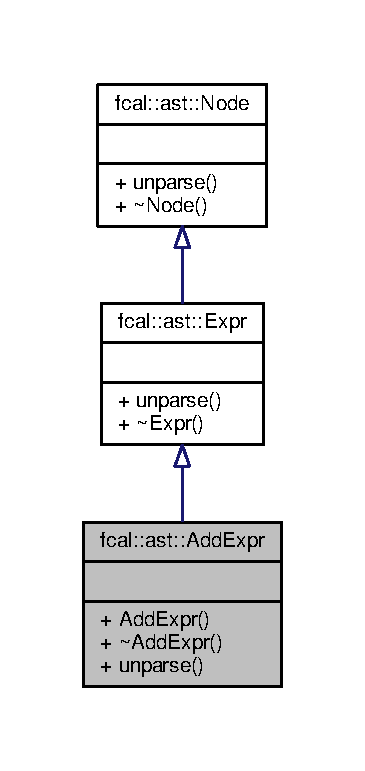
\includegraphics[width=175pt]{classfcal_1_1ast_1_1AddExpr__inherit__graph}
\end{center}
\end{figure}


Collaboration diagram for fcal\+:\+:ast\+:\+:Add\+Expr\+:
\nopagebreak
\begin{figure}[H]
\begin{center}
\leavevmode
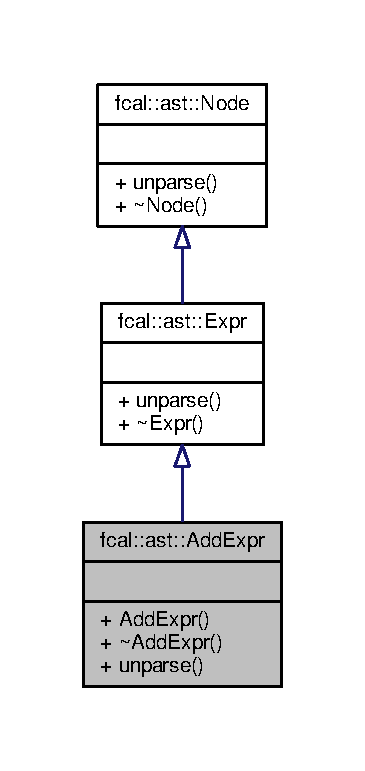
\includegraphics[width=175pt]{classfcal_1_1ast_1_1AddExpr__coll__graph}
\end{center}
\end{figure}
\subsection*{Public Member Functions}
\begin{DoxyCompactItemize}
\item 
\hyperlink{classfcal_1_1ast_1_1AddExpr_a005cbd687ea20133b01c22c32eea9c90}{Add\+Expr} (\hyperlink{classfcal_1_1ast_1_1Expr}{Expr} $\ast$e1, \hyperlink{classfcal_1_1ast_1_1Expr}{Expr} $\ast$e2)
\item 
\hyperlink{classfcal_1_1ast_1_1AddExpr_a91782fde0bf3227f8a459918e7884ef0}{$\sim$\+Add\+Expr} ()
\item 
std\+::string \hyperlink{classfcal_1_1ast_1_1AddExpr_ab091a379ec85a4f0d3861f440d3fb54e}{unparse} ()
\end{DoxyCompactItemize}


\subsection{Constructor \& Destructor Documentation}
\index{fcal\+::ast\+::\+Add\+Expr@{fcal\+::ast\+::\+Add\+Expr}!Add\+Expr@{Add\+Expr}}
\index{Add\+Expr@{Add\+Expr}!fcal\+::ast\+::\+Add\+Expr@{fcal\+::ast\+::\+Add\+Expr}}
\subsubsection[{\texorpdfstring{Add\+Expr(\+Expr $\ast$e1, Expr $\ast$e2)}{AddExpr(Expr *e1, Expr *e2)}}]{\setlength{\rightskip}{0pt plus 5cm}fcal\+::ast\+::\+Add\+Expr\+::\+Add\+Expr (
\begin{DoxyParamCaption}
\item[{{\bf Expr} $\ast$}]{e1, }
\item[{{\bf Expr} $\ast$}]{e2}
\end{DoxyParamCaption}
)\hspace{0.3cm}{\ttfamily [inline]}}\hypertarget{classfcal_1_1ast_1_1AddExpr_a005cbd687ea20133b01c22c32eea9c90}{}\label{classfcal_1_1ast_1_1AddExpr_a005cbd687ea20133b01c22c32eea9c90}
\index{fcal\+::ast\+::\+Add\+Expr@{fcal\+::ast\+::\+Add\+Expr}!````~Add\+Expr@{$\sim$\+Add\+Expr}}
\index{````~Add\+Expr@{$\sim$\+Add\+Expr}!fcal\+::ast\+::\+Add\+Expr@{fcal\+::ast\+::\+Add\+Expr}}
\subsubsection[{\texorpdfstring{$\sim$\+Add\+Expr()}{~AddExpr()}}]{\setlength{\rightskip}{0pt plus 5cm}fcal\+::ast\+::\+Add\+Expr\+::$\sim$\+Add\+Expr (
\begin{DoxyParamCaption}
{}
\end{DoxyParamCaption}
)\hspace{0.3cm}{\ttfamily [inline]}}\hypertarget{classfcal_1_1ast_1_1AddExpr_a91782fde0bf3227f8a459918e7884ef0}{}\label{classfcal_1_1ast_1_1AddExpr_a91782fde0bf3227f8a459918e7884ef0}


\subsection{Member Function Documentation}
\index{fcal\+::ast\+::\+Add\+Expr@{fcal\+::ast\+::\+Add\+Expr}!unparse@{unparse}}
\index{unparse@{unparse}!fcal\+::ast\+::\+Add\+Expr@{fcal\+::ast\+::\+Add\+Expr}}
\subsubsection[{\texorpdfstring{unparse()}{unparse()}}]{\setlength{\rightskip}{0pt plus 5cm}std\+::string fcal\+::ast\+::\+Add\+Expr\+::unparse (
\begin{DoxyParamCaption}
{}
\end{DoxyParamCaption}
)\hspace{0.3cm}{\ttfamily [inline]}, {\ttfamily [virtual]}}\hypertarget{classfcal_1_1ast_1_1AddExpr_ab091a379ec85a4f0d3861f440d3fb54e}{}\label{classfcal_1_1ast_1_1AddExpr_ab091a379ec85a4f0d3861f440d3fb54e}


Implements \hyperlink{classfcal_1_1ast_1_1Expr_adba9309749d00e7c864456fbd505f252}{fcal\+::ast\+::\+Expr}.



The documentation for this class was generated from the following file\+:\begin{DoxyCompactItemize}
\item 
include/\hyperlink{ast_8h}{ast.\+h}\end{DoxyCompactItemize}

\hypertarget{classfcal_1_1ast_1_1AssignStmt}{}\section{fcal\+:\+:ast\+:\+:Assign\+Stmt Class Reference}
\label{classfcal_1_1ast_1_1AssignStmt}\index{fcal\+::ast\+::\+Assign\+Stmt@{fcal\+::ast\+::\+Assign\+Stmt}}


{\ttfamily \#include $<$ast.\+h$>$}



Inheritance diagram for fcal\+:\+:ast\+:\+:Assign\+Stmt\+:
\nopagebreak
\begin{figure}[H]
\begin{center}
\leavevmode
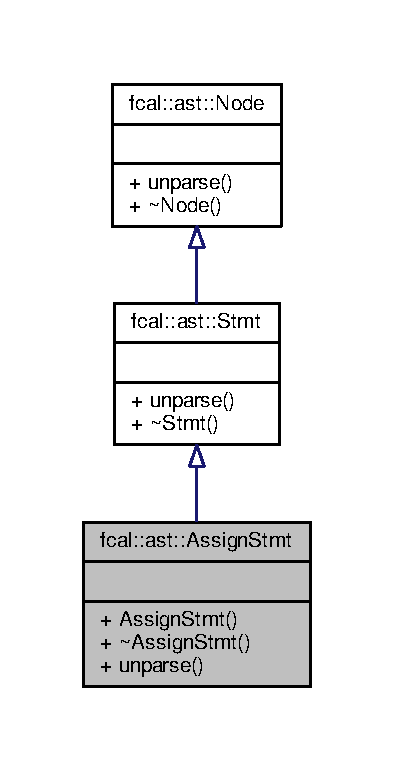
\includegraphics[width=189pt]{classfcal_1_1ast_1_1AssignStmt__inherit__graph}
\end{center}
\end{figure}


Collaboration diagram for fcal\+:\+:ast\+:\+:Assign\+Stmt\+:
\nopagebreak
\begin{figure}[H]
\begin{center}
\leavevmode
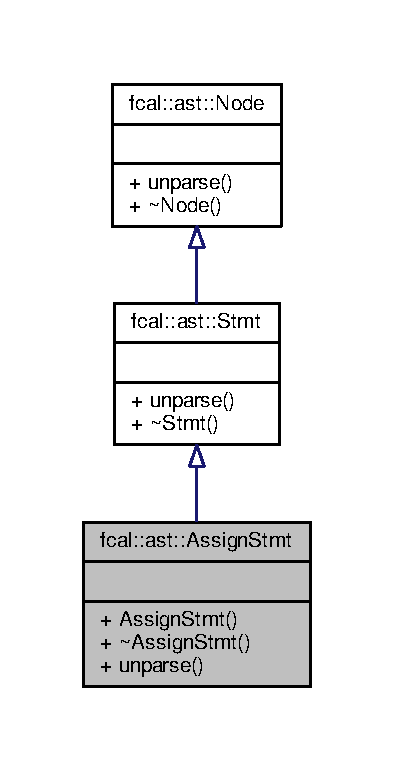
\includegraphics[width=189pt]{classfcal_1_1ast_1_1AssignStmt__coll__graph}
\end{center}
\end{figure}
\subsection*{Public Member Functions}
\begin{DoxyCompactItemize}
\item 
\hyperlink{classfcal_1_1ast_1_1AssignStmt_aa307bda28c28b25f884cdc83cd90ec87}{Assign\+Stmt} (std\+::string v, \hyperlink{classfcal_1_1ast_1_1Expr}{Expr} $\ast$e)
\item 
\hyperlink{classfcal_1_1ast_1_1AssignStmt_afa239c50a03eb775be4429d5629a5217}{$\sim$\+Assign\+Stmt} ()
\item 
std\+::string \hyperlink{classfcal_1_1ast_1_1AssignStmt_ae58f8af8bc26ae0994d95ae266433ded}{unparse} ()
\end{DoxyCompactItemize}


\subsection{Constructor \& Destructor Documentation}
\index{fcal\+::ast\+::\+Assign\+Stmt@{fcal\+::ast\+::\+Assign\+Stmt}!Assign\+Stmt@{Assign\+Stmt}}
\index{Assign\+Stmt@{Assign\+Stmt}!fcal\+::ast\+::\+Assign\+Stmt@{fcal\+::ast\+::\+Assign\+Stmt}}
\subsubsection[{\texorpdfstring{Assign\+Stmt(std\+::string v, Expr $\ast$e)}{AssignStmt(std::string v, Expr *e)}}]{\setlength{\rightskip}{0pt plus 5cm}fcal\+::ast\+::\+Assign\+Stmt\+::\+Assign\+Stmt (
\begin{DoxyParamCaption}
\item[{std\+::string}]{v, }
\item[{{\bf Expr} $\ast$}]{e}
\end{DoxyParamCaption}
)\hspace{0.3cm}{\ttfamily [inline]}}\hypertarget{classfcal_1_1ast_1_1AssignStmt_aa307bda28c28b25f884cdc83cd90ec87}{}\label{classfcal_1_1ast_1_1AssignStmt_aa307bda28c28b25f884cdc83cd90ec87}
\index{fcal\+::ast\+::\+Assign\+Stmt@{fcal\+::ast\+::\+Assign\+Stmt}!````~Assign\+Stmt@{$\sim$\+Assign\+Stmt}}
\index{````~Assign\+Stmt@{$\sim$\+Assign\+Stmt}!fcal\+::ast\+::\+Assign\+Stmt@{fcal\+::ast\+::\+Assign\+Stmt}}
\subsubsection[{\texorpdfstring{$\sim$\+Assign\+Stmt()}{~AssignStmt()}}]{\setlength{\rightskip}{0pt plus 5cm}fcal\+::ast\+::\+Assign\+Stmt\+::$\sim$\+Assign\+Stmt (
\begin{DoxyParamCaption}
{}
\end{DoxyParamCaption}
)\hspace{0.3cm}{\ttfamily [inline]}}\hypertarget{classfcal_1_1ast_1_1AssignStmt_afa239c50a03eb775be4429d5629a5217}{}\label{classfcal_1_1ast_1_1AssignStmt_afa239c50a03eb775be4429d5629a5217}


\subsection{Member Function Documentation}
\index{fcal\+::ast\+::\+Assign\+Stmt@{fcal\+::ast\+::\+Assign\+Stmt}!unparse@{unparse}}
\index{unparse@{unparse}!fcal\+::ast\+::\+Assign\+Stmt@{fcal\+::ast\+::\+Assign\+Stmt}}
\subsubsection[{\texorpdfstring{unparse()}{unparse()}}]{\setlength{\rightskip}{0pt plus 5cm}std\+::string fcal\+::ast\+::\+Assign\+Stmt\+::unparse (
\begin{DoxyParamCaption}
{}
\end{DoxyParamCaption}
)\hspace{0.3cm}{\ttfamily [inline]}, {\ttfamily [virtual]}}\hypertarget{classfcal_1_1ast_1_1AssignStmt_ae58f8af8bc26ae0994d95ae266433ded}{}\label{classfcal_1_1ast_1_1AssignStmt_ae58f8af8bc26ae0994d95ae266433ded}


Implements \hyperlink{classfcal_1_1ast_1_1Stmt_a2ed8595941ddc947012bfeae54f4447d}{fcal\+::ast\+::\+Stmt}.



The documentation for this class was generated from the following file\+:\begin{DoxyCompactItemize}
\item 
include/\hyperlink{ast_8h}{ast.\+h}\end{DoxyCompactItemize}

\hypertarget{classfcal_1_1ast_1_1BooleanConstExpr}{}\section{fcal\+:\+:ast\+:\+:Boolean\+Const\+Expr Class Reference}
\label{classfcal_1_1ast_1_1BooleanConstExpr}\index{fcal\+::ast\+::\+Boolean\+Const\+Expr@{fcal\+::ast\+::\+Boolean\+Const\+Expr}}


{\ttfamily \#include $<$ast.\+h$>$}



Inheritance diagram for fcal\+:\+:ast\+:\+:Boolean\+Const\+Expr\+:
\nopagebreak
\begin{figure}[H]
\begin{center}
\leavevmode
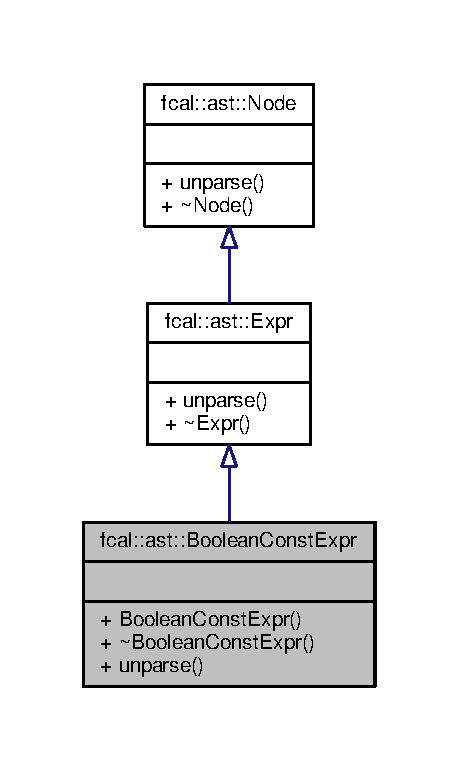
\includegraphics[width=220pt]{classfcal_1_1ast_1_1BooleanConstExpr__inherit__graph}
\end{center}
\end{figure}


Collaboration diagram for fcal\+:\+:ast\+:\+:Boolean\+Const\+Expr\+:
\nopagebreak
\begin{figure}[H]
\begin{center}
\leavevmode
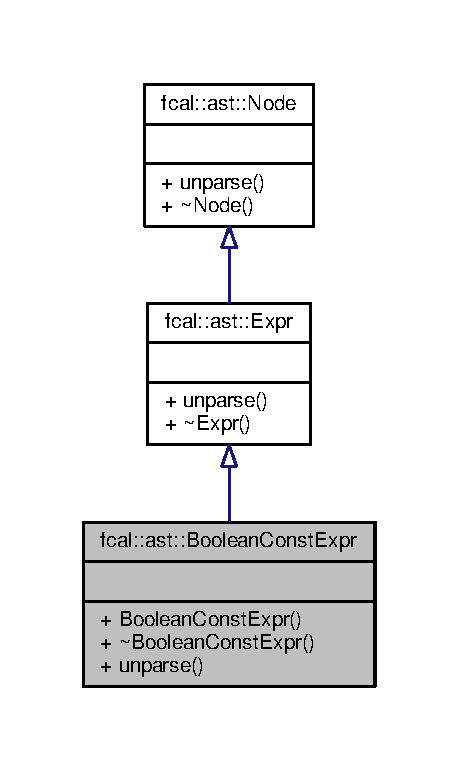
\includegraphics[width=220pt]{classfcal_1_1ast_1_1BooleanConstExpr__coll__graph}
\end{center}
\end{figure}
\subsection*{Public Member Functions}
\begin{DoxyCompactItemize}
\item 
\hyperlink{classfcal_1_1ast_1_1BooleanConstExpr_a456ff1929e3cf2e21d19c53d9f06bec9}{Boolean\+Const\+Expr} (std\+::string b)
\item 
\hyperlink{classfcal_1_1ast_1_1BooleanConstExpr_a7e0f518f983a98f986c7ee2206972400}{$\sim$\+Boolean\+Const\+Expr} ()
\item 
std\+::string \hyperlink{classfcal_1_1ast_1_1BooleanConstExpr_a24fbd101f0aa59fc7379b2365f4f84be}{unparse} ()
\end{DoxyCompactItemize}


\subsection{Constructor \& Destructor Documentation}
\index{fcal\+::ast\+::\+Boolean\+Const\+Expr@{fcal\+::ast\+::\+Boolean\+Const\+Expr}!Boolean\+Const\+Expr@{Boolean\+Const\+Expr}}
\index{Boolean\+Const\+Expr@{Boolean\+Const\+Expr}!fcal\+::ast\+::\+Boolean\+Const\+Expr@{fcal\+::ast\+::\+Boolean\+Const\+Expr}}
\subsubsection[{\texorpdfstring{Boolean\+Const\+Expr(std\+::string b)}{BooleanConstExpr(std::string b)}}]{\setlength{\rightskip}{0pt plus 5cm}fcal\+::ast\+::\+Boolean\+Const\+Expr\+::\+Boolean\+Const\+Expr (
\begin{DoxyParamCaption}
\item[{std\+::string}]{b}
\end{DoxyParamCaption}
)\hspace{0.3cm}{\ttfamily [inline]}, {\ttfamily [explicit]}}\hypertarget{classfcal_1_1ast_1_1BooleanConstExpr_a456ff1929e3cf2e21d19c53d9f06bec9}{}\label{classfcal_1_1ast_1_1BooleanConstExpr_a456ff1929e3cf2e21d19c53d9f06bec9}
\index{fcal\+::ast\+::\+Boolean\+Const\+Expr@{fcal\+::ast\+::\+Boolean\+Const\+Expr}!````~Boolean\+Const\+Expr@{$\sim$\+Boolean\+Const\+Expr}}
\index{````~Boolean\+Const\+Expr@{$\sim$\+Boolean\+Const\+Expr}!fcal\+::ast\+::\+Boolean\+Const\+Expr@{fcal\+::ast\+::\+Boolean\+Const\+Expr}}
\subsubsection[{\texorpdfstring{$\sim$\+Boolean\+Const\+Expr()}{~BooleanConstExpr()}}]{\setlength{\rightskip}{0pt plus 5cm}fcal\+::ast\+::\+Boolean\+Const\+Expr\+::$\sim$\+Boolean\+Const\+Expr (
\begin{DoxyParamCaption}
{}
\end{DoxyParamCaption}
)\hspace{0.3cm}{\ttfamily [inline]}}\hypertarget{classfcal_1_1ast_1_1BooleanConstExpr_a7e0f518f983a98f986c7ee2206972400}{}\label{classfcal_1_1ast_1_1BooleanConstExpr_a7e0f518f983a98f986c7ee2206972400}


\subsection{Member Function Documentation}
\index{fcal\+::ast\+::\+Boolean\+Const\+Expr@{fcal\+::ast\+::\+Boolean\+Const\+Expr}!unparse@{unparse}}
\index{unparse@{unparse}!fcal\+::ast\+::\+Boolean\+Const\+Expr@{fcal\+::ast\+::\+Boolean\+Const\+Expr}}
\subsubsection[{\texorpdfstring{unparse()}{unparse()}}]{\setlength{\rightskip}{0pt plus 5cm}std\+::string fcal\+::ast\+::\+Boolean\+Const\+Expr\+::unparse (
\begin{DoxyParamCaption}
{}
\end{DoxyParamCaption}
)\hspace{0.3cm}{\ttfamily [inline]}, {\ttfamily [virtual]}}\hypertarget{classfcal_1_1ast_1_1BooleanConstExpr_a24fbd101f0aa59fc7379b2365f4f84be}{}\label{classfcal_1_1ast_1_1BooleanConstExpr_a24fbd101f0aa59fc7379b2365f4f84be}


Implements \hyperlink{classfcal_1_1ast_1_1Expr_adba9309749d00e7c864456fbd505f252}{fcal\+::ast\+::\+Expr}.



The documentation for this class was generated from the following file\+:\begin{DoxyCompactItemize}
\item 
include/\hyperlink{ast_8h}{ast.\+h}\end{DoxyCompactItemize}

\hypertarget{classfcal_1_1ast_1_1BooleanDecl}{}\section{fcal\+:\+:ast\+:\+:Boolean\+Decl Class Reference}
\label{classfcal_1_1ast_1_1BooleanDecl}\index{fcal\+::ast\+::\+Boolean\+Decl@{fcal\+::ast\+::\+Boolean\+Decl}}


{\ttfamily \#include $<$ast.\+h$>$}



Inheritance diagram for fcal\+:\+:ast\+:\+:Boolean\+Decl\+:
\nopagebreak
\begin{figure}[H]
\begin{center}
\leavevmode
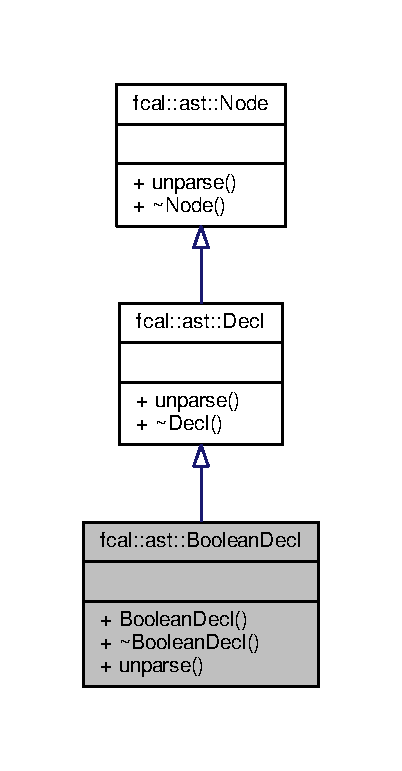
\includegraphics[width=193pt]{classfcal_1_1ast_1_1BooleanDecl__inherit__graph}
\end{center}
\end{figure}


Collaboration diagram for fcal\+:\+:ast\+:\+:Boolean\+Decl\+:
\nopagebreak
\begin{figure}[H]
\begin{center}
\leavevmode
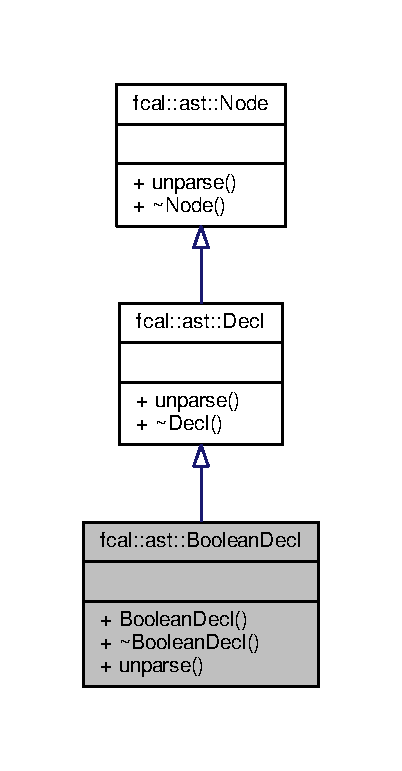
\includegraphics[width=193pt]{classfcal_1_1ast_1_1BooleanDecl__coll__graph}
\end{center}
\end{figure}
\subsection*{Public Member Functions}
\begin{DoxyCompactItemize}
\item 
\hyperlink{classfcal_1_1ast_1_1BooleanDecl_a963be5fff559039b7200f6160e40c91b}{Boolean\+Decl} (std\+::string s)
\item 
\hyperlink{classfcal_1_1ast_1_1BooleanDecl_a84df7f6e1819fdfa6ef4329a32a81931}{$\sim$\+Boolean\+Decl} ()
\item 
std\+::string \hyperlink{classfcal_1_1ast_1_1BooleanDecl_a6f7b128adddaf89386c3b266f3fa0198}{unparse} ()
\end{DoxyCompactItemize}


\subsection{Constructor \& Destructor Documentation}
\index{fcal\+::ast\+::\+Boolean\+Decl@{fcal\+::ast\+::\+Boolean\+Decl}!Boolean\+Decl@{Boolean\+Decl}}
\index{Boolean\+Decl@{Boolean\+Decl}!fcal\+::ast\+::\+Boolean\+Decl@{fcal\+::ast\+::\+Boolean\+Decl}}
\subsubsection[{\texorpdfstring{Boolean\+Decl(std\+::string s)}{BooleanDecl(std::string s)}}]{\setlength{\rightskip}{0pt plus 5cm}fcal\+::ast\+::\+Boolean\+Decl\+::\+Boolean\+Decl (
\begin{DoxyParamCaption}
\item[{std\+::string}]{s}
\end{DoxyParamCaption}
)\hspace{0.3cm}{\ttfamily [inline]}, {\ttfamily [explicit]}}\hypertarget{classfcal_1_1ast_1_1BooleanDecl_a963be5fff559039b7200f6160e40c91b}{}\label{classfcal_1_1ast_1_1BooleanDecl_a963be5fff559039b7200f6160e40c91b}
\index{fcal\+::ast\+::\+Boolean\+Decl@{fcal\+::ast\+::\+Boolean\+Decl}!````~Boolean\+Decl@{$\sim$\+Boolean\+Decl}}
\index{````~Boolean\+Decl@{$\sim$\+Boolean\+Decl}!fcal\+::ast\+::\+Boolean\+Decl@{fcal\+::ast\+::\+Boolean\+Decl}}
\subsubsection[{\texorpdfstring{$\sim$\+Boolean\+Decl()}{~BooleanDecl()}}]{\setlength{\rightskip}{0pt plus 5cm}fcal\+::ast\+::\+Boolean\+Decl\+::$\sim$\+Boolean\+Decl (
\begin{DoxyParamCaption}
{}
\end{DoxyParamCaption}
)\hspace{0.3cm}{\ttfamily [inline]}}\hypertarget{classfcal_1_1ast_1_1BooleanDecl_a84df7f6e1819fdfa6ef4329a32a81931}{}\label{classfcal_1_1ast_1_1BooleanDecl_a84df7f6e1819fdfa6ef4329a32a81931}


\subsection{Member Function Documentation}
\index{fcal\+::ast\+::\+Boolean\+Decl@{fcal\+::ast\+::\+Boolean\+Decl}!unparse@{unparse}}
\index{unparse@{unparse}!fcal\+::ast\+::\+Boolean\+Decl@{fcal\+::ast\+::\+Boolean\+Decl}}
\subsubsection[{\texorpdfstring{unparse()}{unparse()}}]{\setlength{\rightskip}{0pt plus 5cm}std\+::string fcal\+::ast\+::\+Boolean\+Decl\+::unparse (
\begin{DoxyParamCaption}
{}
\end{DoxyParamCaption}
)\hspace{0.3cm}{\ttfamily [inline]}, {\ttfamily [virtual]}}\hypertarget{classfcal_1_1ast_1_1BooleanDecl_a6f7b128adddaf89386c3b266f3fa0198}{}\label{classfcal_1_1ast_1_1BooleanDecl_a6f7b128adddaf89386c3b266f3fa0198}


Implements \hyperlink{classfcal_1_1ast_1_1Decl_a54761cf8b990cb2d478c606be6bc29c5}{fcal\+::ast\+::\+Decl}.



The documentation for this class was generated from the following file\+:\begin{DoxyCompactItemize}
\item 
include/\hyperlink{ast_8h}{ast.\+h}\end{DoxyCompactItemize}

\hypertarget{classfcal_1_1ast_1_1BracketsStmt}{}\section{fcal\+:\+:ast\+:\+:Brackets\+Stmt Class Reference}
\label{classfcal_1_1ast_1_1BracketsStmt}\index{fcal\+::ast\+::\+Brackets\+Stmt@{fcal\+::ast\+::\+Brackets\+Stmt}}


{\ttfamily \#include $<$ast.\+h$>$}



Inheritance diagram for fcal\+:\+:ast\+:\+:Brackets\+Stmt\+:
\nopagebreak
\begin{figure}[H]
\begin{center}
\leavevmode
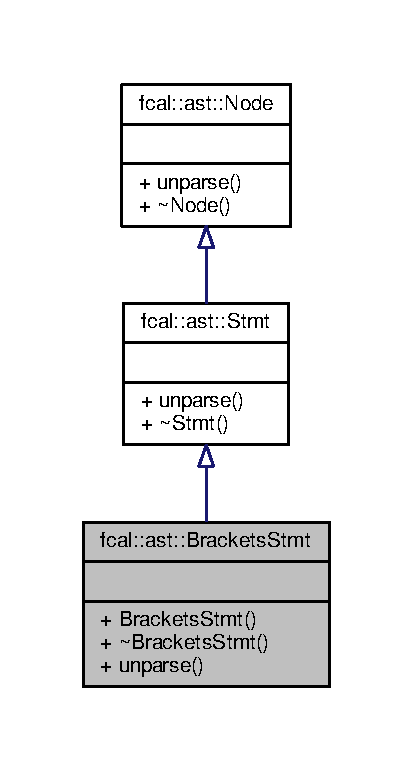
\includegraphics[width=198pt]{classfcal_1_1ast_1_1BracketsStmt__inherit__graph}
\end{center}
\end{figure}


Collaboration diagram for fcal\+:\+:ast\+:\+:Brackets\+Stmt\+:
\nopagebreak
\begin{figure}[H]
\begin{center}
\leavevmode
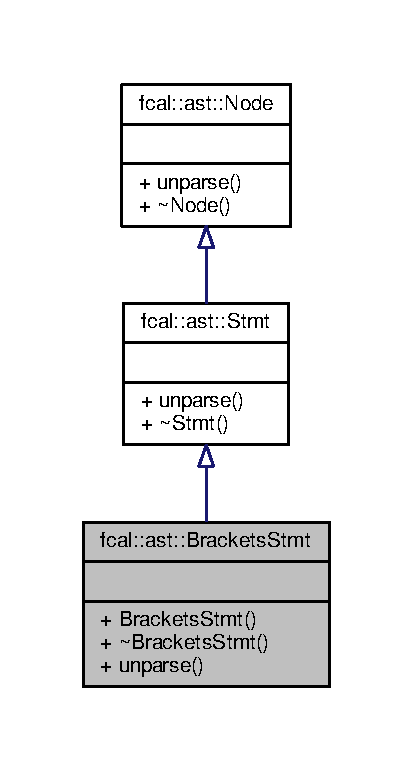
\includegraphics[width=198pt]{classfcal_1_1ast_1_1BracketsStmt__coll__graph}
\end{center}
\end{figure}
\subsection*{Public Member Functions}
\begin{DoxyCompactItemize}
\item 
\hyperlink{classfcal_1_1ast_1_1BracketsStmt_acd73a437dde409574c433221b3e16b62}{Brackets\+Stmt} (\hyperlink{classfcal_1_1ast_1_1Stmts}{Stmts} $\ast$s)
\item 
\hyperlink{classfcal_1_1ast_1_1BracketsStmt_acc226fdb915d61b35e18505587333e63}{$\sim$\+Brackets\+Stmt} ()
\item 
std\+::string \hyperlink{classfcal_1_1ast_1_1BracketsStmt_a1779d8a9115bd9ef4fb6835e45509573}{unparse} ()
\end{DoxyCompactItemize}


\subsection{Constructor \& Destructor Documentation}
\index{fcal\+::ast\+::\+Brackets\+Stmt@{fcal\+::ast\+::\+Brackets\+Stmt}!Brackets\+Stmt@{Brackets\+Stmt}}
\index{Brackets\+Stmt@{Brackets\+Stmt}!fcal\+::ast\+::\+Brackets\+Stmt@{fcal\+::ast\+::\+Brackets\+Stmt}}
\subsubsection[{\texorpdfstring{Brackets\+Stmt(\+Stmts $\ast$s)}{BracketsStmt(Stmts *s)}}]{\setlength{\rightskip}{0pt plus 5cm}fcal\+::ast\+::\+Brackets\+Stmt\+::\+Brackets\+Stmt (
\begin{DoxyParamCaption}
\item[{{\bf Stmts} $\ast$}]{s}
\end{DoxyParamCaption}
)\hspace{0.3cm}{\ttfamily [inline]}, {\ttfamily [explicit]}}\hypertarget{classfcal_1_1ast_1_1BracketsStmt_acd73a437dde409574c433221b3e16b62}{}\label{classfcal_1_1ast_1_1BracketsStmt_acd73a437dde409574c433221b3e16b62}
\index{fcal\+::ast\+::\+Brackets\+Stmt@{fcal\+::ast\+::\+Brackets\+Stmt}!````~Brackets\+Stmt@{$\sim$\+Brackets\+Stmt}}
\index{````~Brackets\+Stmt@{$\sim$\+Brackets\+Stmt}!fcal\+::ast\+::\+Brackets\+Stmt@{fcal\+::ast\+::\+Brackets\+Stmt}}
\subsubsection[{\texorpdfstring{$\sim$\+Brackets\+Stmt()}{~BracketsStmt()}}]{\setlength{\rightskip}{0pt plus 5cm}fcal\+::ast\+::\+Brackets\+Stmt\+::$\sim$\+Brackets\+Stmt (
\begin{DoxyParamCaption}
{}
\end{DoxyParamCaption}
)\hspace{0.3cm}{\ttfamily [inline]}}\hypertarget{classfcal_1_1ast_1_1BracketsStmt_acc226fdb915d61b35e18505587333e63}{}\label{classfcal_1_1ast_1_1BracketsStmt_acc226fdb915d61b35e18505587333e63}


\subsection{Member Function Documentation}
\index{fcal\+::ast\+::\+Brackets\+Stmt@{fcal\+::ast\+::\+Brackets\+Stmt}!unparse@{unparse}}
\index{unparse@{unparse}!fcal\+::ast\+::\+Brackets\+Stmt@{fcal\+::ast\+::\+Brackets\+Stmt}}
\subsubsection[{\texorpdfstring{unparse()}{unparse()}}]{\setlength{\rightskip}{0pt plus 5cm}std\+::string fcal\+::ast\+::\+Brackets\+Stmt\+::unparse (
\begin{DoxyParamCaption}
{}
\end{DoxyParamCaption}
)\hspace{0.3cm}{\ttfamily [inline]}, {\ttfamily [virtual]}}\hypertarget{classfcal_1_1ast_1_1BracketsStmt_a1779d8a9115bd9ef4fb6835e45509573}{}\label{classfcal_1_1ast_1_1BracketsStmt_a1779d8a9115bd9ef4fb6835e45509573}


Implements \hyperlink{classfcal_1_1ast_1_1Stmt_a2ed8595941ddc947012bfeae54f4447d}{fcal\+::ast\+::\+Stmt}.



The documentation for this class was generated from the following file\+:\begin{DoxyCompactItemize}
\item 
include/\hyperlink{ast_8h}{ast.\+h}\end{DoxyCompactItemize}

\hypertarget{classfcal_1_1scanner_1_1CharConstToken}{}\section{fcal\+:\+:scanner\+:\+:Char\+Const\+Token Class Reference}
\label{classfcal_1_1scanner_1_1CharConstToken}\index{fcal\+::scanner\+::\+Char\+Const\+Token@{fcal\+::scanner\+::\+Char\+Const\+Token}}


{\ttfamily \#include $<$ext\+\_\+token.\+h$>$}



Inheritance diagram for fcal\+:\+:scanner\+:\+:Char\+Const\+Token\+:
\nopagebreak
\begin{figure}[H]
\begin{center}
\leavevmode
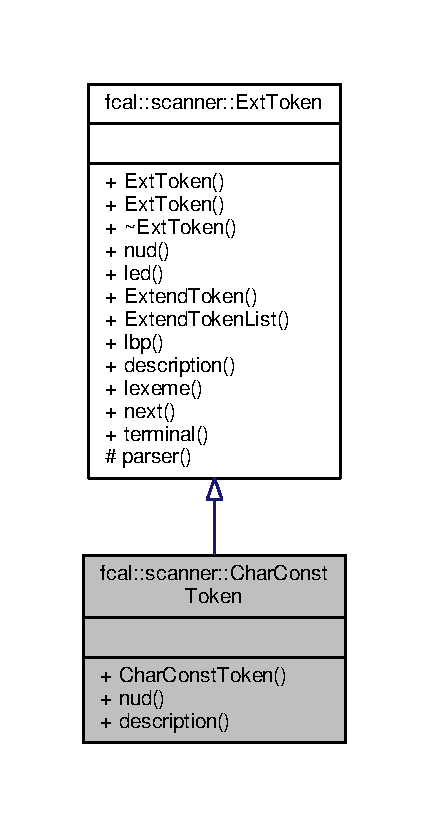
\includegraphics[width=206pt]{classfcal_1_1scanner_1_1CharConstToken__inherit__graph}
\end{center}
\end{figure}


Collaboration diagram for fcal\+:\+:scanner\+:\+:Char\+Const\+Token\+:
\nopagebreak
\begin{figure}[H]
\begin{center}
\leavevmode
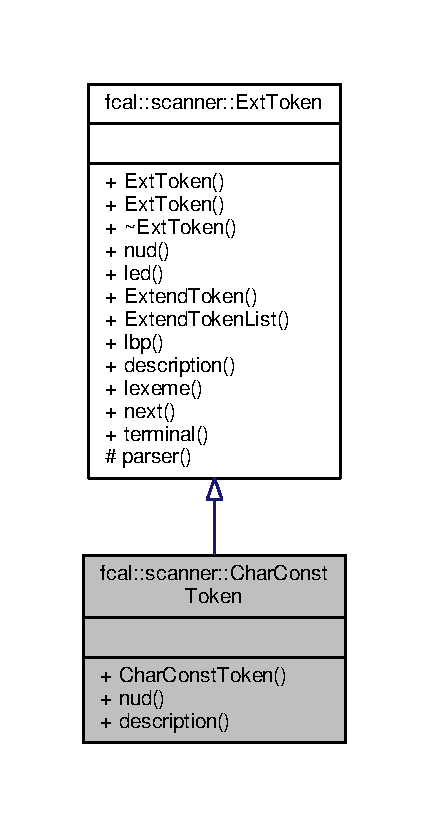
\includegraphics[width=206pt]{classfcal_1_1scanner_1_1CharConstToken__coll__graph}
\end{center}
\end{figure}
\subsection*{Public Member Functions}
\begin{DoxyCompactItemize}
\item 
\hyperlink{classfcal_1_1scanner_1_1CharConstToken_ae108041381482344ee7cf3bf0629fbba}{Char\+Const\+Token} (\hyperlink{classfcal_1_1parser_1_1Parser}{parser\+::\+Parser} $\ast$p, \hyperlink{classfcal_1_1scanner_1_1Token}{Token} $\ast$t)
\item 
\hyperlink{classfcal_1_1parser_1_1ParseResult}{parser\+::\+Parse\+Result} \hyperlink{classfcal_1_1scanner_1_1CharConstToken_a5e9299e684f969cde0f71c0041e92153}{nud} ()
\item 
std\+::string \hyperlink{classfcal_1_1scanner_1_1CharConstToken_a283d5fb12d36caac1afed73c1035b562}{description} ()
\end{DoxyCompactItemize}
\subsection*{Additional Inherited Members}


\subsection{Constructor \& Destructor Documentation}
\index{fcal\+::scanner\+::\+Char\+Const\+Token@{fcal\+::scanner\+::\+Char\+Const\+Token}!Char\+Const\+Token@{Char\+Const\+Token}}
\index{Char\+Const\+Token@{Char\+Const\+Token}!fcal\+::scanner\+::\+Char\+Const\+Token@{fcal\+::scanner\+::\+Char\+Const\+Token}}
\subsubsection[{\texorpdfstring{Char\+Const\+Token(parser\+::\+Parser $\ast$p, Token $\ast$t)}{CharConstToken(parser::Parser *p, Token *t)}}]{\setlength{\rightskip}{0pt plus 5cm}fcal\+::scanner\+::\+Char\+Const\+Token\+::\+Char\+Const\+Token (
\begin{DoxyParamCaption}
\item[{{\bf parser\+::\+Parser} $\ast$}]{p, }
\item[{{\bf Token} $\ast$}]{t}
\end{DoxyParamCaption}
)\hspace{0.3cm}{\ttfamily [inline]}}\hypertarget{classfcal_1_1scanner_1_1CharConstToken_ae108041381482344ee7cf3bf0629fbba}{}\label{classfcal_1_1scanner_1_1CharConstToken_ae108041381482344ee7cf3bf0629fbba}


\subsection{Member Function Documentation}
\index{fcal\+::scanner\+::\+Char\+Const\+Token@{fcal\+::scanner\+::\+Char\+Const\+Token}!description@{description}}
\index{description@{description}!fcal\+::scanner\+::\+Char\+Const\+Token@{fcal\+::scanner\+::\+Char\+Const\+Token}}
\subsubsection[{\texorpdfstring{description()}{description()}}]{\setlength{\rightskip}{0pt plus 5cm}std\+::string fcal\+::scanner\+::\+Char\+Const\+Token\+::description (
\begin{DoxyParamCaption}
{}
\end{DoxyParamCaption}
)\hspace{0.3cm}{\ttfamily [inline]}, {\ttfamily [virtual]}}\hypertarget{classfcal_1_1scanner_1_1CharConstToken_a283d5fb12d36caac1afed73c1035b562}{}\label{classfcal_1_1scanner_1_1CharConstToken_a283d5fb12d36caac1afed73c1035b562}


Reimplemented from \hyperlink{classfcal_1_1scanner_1_1ExtToken_a29a72149492d7fef7968a1b894d334c7}{fcal\+::scanner\+::\+Ext\+Token}.

\index{fcal\+::scanner\+::\+Char\+Const\+Token@{fcal\+::scanner\+::\+Char\+Const\+Token}!nud@{nud}}
\index{nud@{nud}!fcal\+::scanner\+::\+Char\+Const\+Token@{fcal\+::scanner\+::\+Char\+Const\+Token}}
\subsubsection[{\texorpdfstring{nud()}{nud()}}]{\setlength{\rightskip}{0pt plus 5cm}{\bf parser\+::\+Parse\+Result} fcal\+::scanner\+::\+Char\+Const\+Token\+::nud (
\begin{DoxyParamCaption}
\item[{void}]{}
\end{DoxyParamCaption}
)\hspace{0.3cm}{\ttfamily [inline]}, {\ttfamily [virtual]}}\hypertarget{classfcal_1_1scanner_1_1CharConstToken_a5e9299e684f969cde0f71c0041e92153}{}\label{classfcal_1_1scanner_1_1CharConstToken_a5e9299e684f969cde0f71c0041e92153}


Reimplemented from \hyperlink{classfcal_1_1scanner_1_1ExtToken_a2e1ca27a07d55593ffd67780dbcad7dd}{fcal\+::scanner\+::\+Ext\+Token}.



The documentation for this class was generated from the following file\+:\begin{DoxyCompactItemize}
\item 
include/\hyperlink{ext__token_8h}{ext\+\_\+token.\+h}\end{DoxyCompactItemize}

\hypertarget{classfcal_1_1scanner_1_1DashToken}{}\section{fcal\+:\+:scanner\+:\+:Dash\+Token Class Reference}
\label{classfcal_1_1scanner_1_1DashToken}\index{fcal\+::scanner\+::\+Dash\+Token@{fcal\+::scanner\+::\+Dash\+Token}}


{\ttfamily \#include $<$ext\+\_\+token.\+h$>$}



Inheritance diagram for fcal\+:\+:scanner\+:\+:Dash\+Token\+:
\nopagebreak
\begin{figure}[H]
\begin{center}
\leavevmode
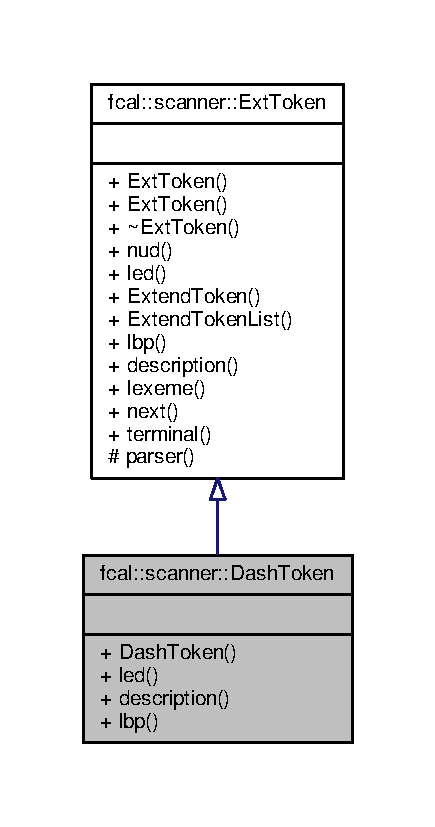
\includegraphics[width=209pt]{classfcal_1_1scanner_1_1DashToken__inherit__graph}
\end{center}
\end{figure}


Collaboration diagram for fcal\+:\+:scanner\+:\+:Dash\+Token\+:
\nopagebreak
\begin{figure}[H]
\begin{center}
\leavevmode
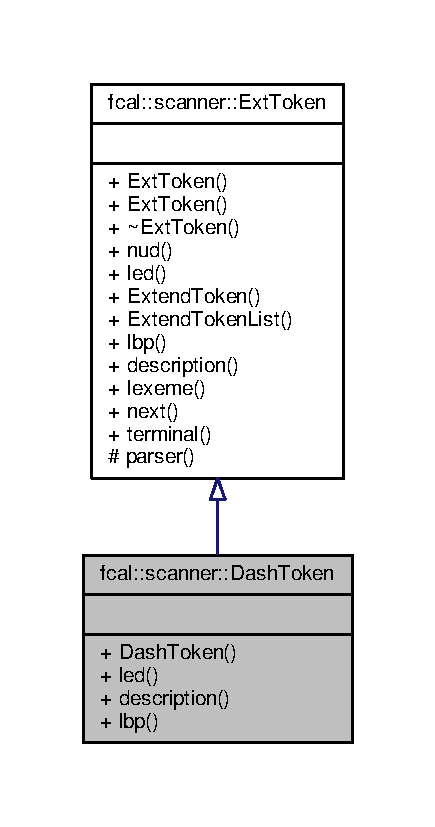
\includegraphics[width=209pt]{classfcal_1_1scanner_1_1DashToken__coll__graph}
\end{center}
\end{figure}
\subsection*{Public Member Functions}
\begin{DoxyCompactItemize}
\item 
\hyperlink{classfcal_1_1scanner_1_1DashToken_afaabbf1a78e35a4592cd8a5e1bfab79f}{Dash\+Token} (\hyperlink{classfcal_1_1parser_1_1Parser}{parser\+::\+Parser} $\ast$p, \hyperlink{classfcal_1_1scanner_1_1Token}{Token} $\ast$t)
\item 
\hyperlink{classfcal_1_1parser_1_1ParseResult}{parser\+::\+Parse\+Result} \hyperlink{classfcal_1_1scanner_1_1DashToken_a7c0e98c83937cf698ce6f32380e17c52}{led} (\hyperlink{classfcal_1_1parser_1_1ParseResult}{parser\+::\+Parse\+Result} left)
\item 
std\+::string \hyperlink{classfcal_1_1scanner_1_1DashToken_a87476e28739d1c9966ed330ba8154342}{description} ()
\item 
int \hyperlink{classfcal_1_1scanner_1_1DashToken_a1b88432765ae6c30be1250015ebaa2c4}{lbp} ()
\end{DoxyCompactItemize}
\subsection*{Additional Inherited Members}


\subsection{Constructor \& Destructor Documentation}
\index{fcal\+::scanner\+::\+Dash\+Token@{fcal\+::scanner\+::\+Dash\+Token}!Dash\+Token@{Dash\+Token}}
\index{Dash\+Token@{Dash\+Token}!fcal\+::scanner\+::\+Dash\+Token@{fcal\+::scanner\+::\+Dash\+Token}}
\subsubsection[{\texorpdfstring{Dash\+Token(parser\+::\+Parser $\ast$p, Token $\ast$t)}{DashToken(parser::Parser *p, Token *t)}}]{\setlength{\rightskip}{0pt plus 5cm}fcal\+::scanner\+::\+Dash\+Token\+::\+Dash\+Token (
\begin{DoxyParamCaption}
\item[{{\bf parser\+::\+Parser} $\ast$}]{p, }
\item[{{\bf Token} $\ast$}]{t}
\end{DoxyParamCaption}
)\hspace{0.3cm}{\ttfamily [inline]}}\hypertarget{classfcal_1_1scanner_1_1DashToken_afaabbf1a78e35a4592cd8a5e1bfab79f}{}\label{classfcal_1_1scanner_1_1DashToken_afaabbf1a78e35a4592cd8a5e1bfab79f}


\subsection{Member Function Documentation}
\index{fcal\+::scanner\+::\+Dash\+Token@{fcal\+::scanner\+::\+Dash\+Token}!description@{description}}
\index{description@{description}!fcal\+::scanner\+::\+Dash\+Token@{fcal\+::scanner\+::\+Dash\+Token}}
\subsubsection[{\texorpdfstring{description()}{description()}}]{\setlength{\rightskip}{0pt plus 5cm}std\+::string fcal\+::scanner\+::\+Dash\+Token\+::description (
\begin{DoxyParamCaption}
{}
\end{DoxyParamCaption}
)\hspace{0.3cm}{\ttfamily [inline]}, {\ttfamily [virtual]}}\hypertarget{classfcal_1_1scanner_1_1DashToken_a87476e28739d1c9966ed330ba8154342}{}\label{classfcal_1_1scanner_1_1DashToken_a87476e28739d1c9966ed330ba8154342}


Reimplemented from \hyperlink{classfcal_1_1scanner_1_1ExtToken_a29a72149492d7fef7968a1b894d334c7}{fcal\+::scanner\+::\+Ext\+Token}.

\index{fcal\+::scanner\+::\+Dash\+Token@{fcal\+::scanner\+::\+Dash\+Token}!lbp@{lbp}}
\index{lbp@{lbp}!fcal\+::scanner\+::\+Dash\+Token@{fcal\+::scanner\+::\+Dash\+Token}}
\subsubsection[{\texorpdfstring{lbp()}{lbp()}}]{\setlength{\rightskip}{0pt plus 5cm}int fcal\+::scanner\+::\+Dash\+Token\+::lbp (
\begin{DoxyParamCaption}
{}
\end{DoxyParamCaption}
)\hspace{0.3cm}{\ttfamily [inline]}, {\ttfamily [virtual]}}\hypertarget{classfcal_1_1scanner_1_1DashToken_a1b88432765ae6c30be1250015ebaa2c4}{}\label{classfcal_1_1scanner_1_1DashToken_a1b88432765ae6c30be1250015ebaa2c4}


Reimplemented from \hyperlink{classfcal_1_1scanner_1_1ExtToken_adecef3770f08e5a26f103ab62171cc91}{fcal\+::scanner\+::\+Ext\+Token}.

\index{fcal\+::scanner\+::\+Dash\+Token@{fcal\+::scanner\+::\+Dash\+Token}!led@{led}}
\index{led@{led}!fcal\+::scanner\+::\+Dash\+Token@{fcal\+::scanner\+::\+Dash\+Token}}
\subsubsection[{\texorpdfstring{led(parser\+::\+Parse\+Result left)}{led(parser::ParseResult left)}}]{\setlength{\rightskip}{0pt plus 5cm}{\bf parser\+::\+Parse\+Result} fcal\+::scanner\+::\+Dash\+Token\+::led (
\begin{DoxyParamCaption}
\item[{{\bf parser\+::\+Parse\+Result}}]{left}
\end{DoxyParamCaption}
)\hspace{0.3cm}{\ttfamily [inline]}, {\ttfamily [virtual]}}\hypertarget{classfcal_1_1scanner_1_1DashToken_a7c0e98c83937cf698ce6f32380e17c52}{}\label{classfcal_1_1scanner_1_1DashToken_a7c0e98c83937cf698ce6f32380e17c52}


Reimplemented from \hyperlink{classfcal_1_1scanner_1_1ExtToken_a42c352ef5e019a1155be80b4a40deb38}{fcal\+::scanner\+::\+Ext\+Token}.



The documentation for this class was generated from the following file\+:\begin{DoxyCompactItemize}
\item 
include/\hyperlink{ext__token_8h}{ext\+\_\+token.\+h}\end{DoxyCompactItemize}

\hypertarget{classfcal_1_1ast_1_1Decl}{}\section{fcal\+:\+:ast\+:\+:Decl Class Reference}
\label{classfcal_1_1ast_1_1Decl}\index{fcal\+::ast\+::\+Decl@{fcal\+::ast\+::\+Decl}}


{\ttfamily \#include $<$ast.\+h$>$}



Inheritance diagram for fcal\+:\+:ast\+:\+:Decl\+:
\nopagebreak
\begin{figure}[H]
\begin{center}
\leavevmode
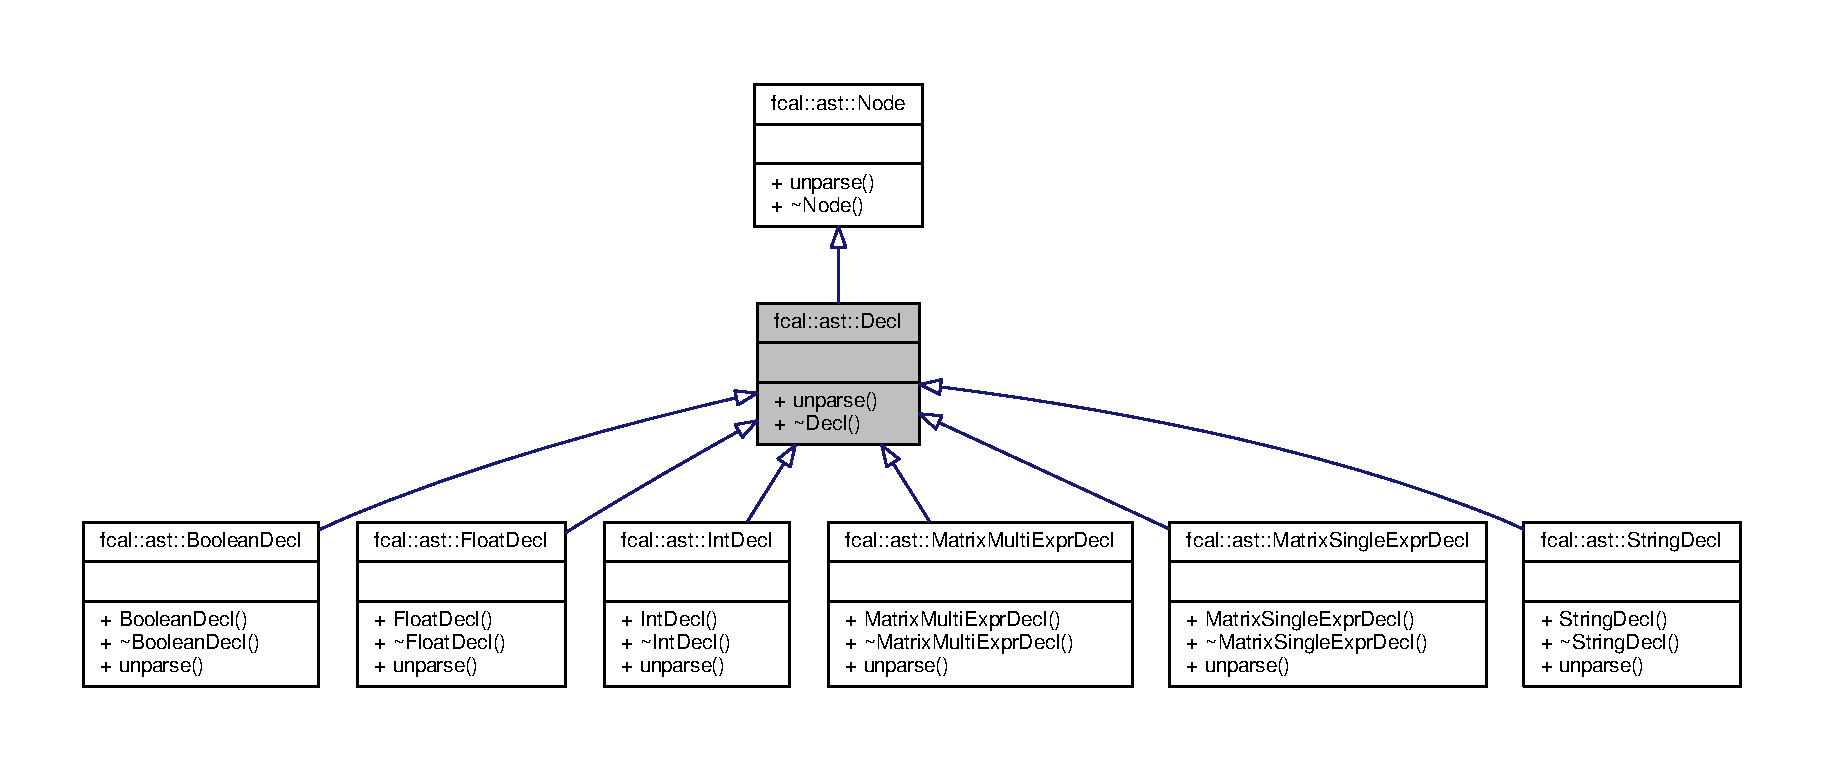
\includegraphics[width=350pt]{classfcal_1_1ast_1_1Decl__inherit__graph}
\end{center}
\end{figure}


Collaboration diagram for fcal\+:\+:ast\+:\+:Decl\+:
\nopagebreak
\begin{figure}[H]
\begin{center}
\leavevmode
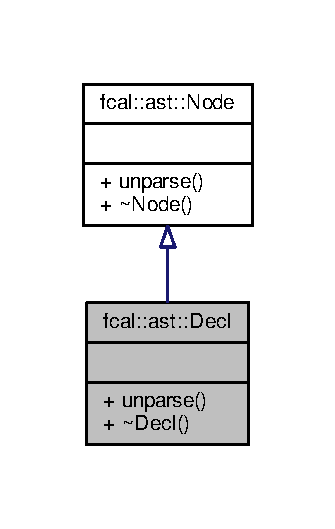
\includegraphics[width=161pt]{classfcal_1_1ast_1_1Decl__coll__graph}
\end{center}
\end{figure}
\subsection*{Public Member Functions}
\begin{DoxyCompactItemize}
\item 
virtual std\+::string \hyperlink{classfcal_1_1ast_1_1Decl_a54761cf8b990cb2d478c606be6bc29c5}{unparse} ()=0
\item 
virtual \hyperlink{classfcal_1_1ast_1_1Decl_ab93bdb6022468e815231cd517d60680f}{$\sim$\+Decl} ()
\end{DoxyCompactItemize}


\subsection{Constructor \& Destructor Documentation}
\index{fcal\+::ast\+::\+Decl@{fcal\+::ast\+::\+Decl}!````~Decl@{$\sim$\+Decl}}
\index{````~Decl@{$\sim$\+Decl}!fcal\+::ast\+::\+Decl@{fcal\+::ast\+::\+Decl}}
\subsubsection[{\texorpdfstring{$\sim$\+Decl()}{~Decl()}}]{\setlength{\rightskip}{0pt plus 5cm}virtual fcal\+::ast\+::\+Decl\+::$\sim$\+Decl (
\begin{DoxyParamCaption}
{}
\end{DoxyParamCaption}
)\hspace{0.3cm}{\ttfamily [inline]}, {\ttfamily [virtual]}}\hypertarget{classfcal_1_1ast_1_1Decl_ab93bdb6022468e815231cd517d60680f}{}\label{classfcal_1_1ast_1_1Decl_ab93bdb6022468e815231cd517d60680f}


\subsection{Member Function Documentation}
\index{fcal\+::ast\+::\+Decl@{fcal\+::ast\+::\+Decl}!unparse@{unparse}}
\index{unparse@{unparse}!fcal\+::ast\+::\+Decl@{fcal\+::ast\+::\+Decl}}
\subsubsection[{\texorpdfstring{unparse()=0}{unparse()=0}}]{\setlength{\rightskip}{0pt plus 5cm}virtual std\+::string fcal\+::ast\+::\+Decl\+::unparse (
\begin{DoxyParamCaption}
{}
\end{DoxyParamCaption}
)\hspace{0.3cm}{\ttfamily [pure virtual]}}\hypertarget{classfcal_1_1ast_1_1Decl_a54761cf8b990cb2d478c606be6bc29c5}{}\label{classfcal_1_1ast_1_1Decl_a54761cf8b990cb2d478c606be6bc29c5}


Implements \hyperlink{classfcal_1_1ast_1_1Node_a81865f5a1df593708a39bf492952742a}{fcal\+::ast\+::\+Node}.



Implemented in \hyperlink{classfcal_1_1ast_1_1MatrixSingleExprDecl_a3c983adc4f904b051d6f908a9c6da76e}{fcal\+::ast\+::\+Matrix\+Single\+Expr\+Decl}, \hyperlink{classfcal_1_1ast_1_1MatrixMultiExprDecl_abb442f53c459332a7168f2153b3f11e9}{fcal\+::ast\+::\+Matrix\+Multi\+Expr\+Decl}, \hyperlink{classfcal_1_1ast_1_1BooleanDecl_a6f7b128adddaf89386c3b266f3fa0198}{fcal\+::ast\+::\+Boolean\+Decl}, \hyperlink{classfcal_1_1ast_1_1StringDecl_a51032ea2eab202f11fb1dc08bd718153}{fcal\+::ast\+::\+String\+Decl}, \hyperlink{classfcal_1_1ast_1_1FloatDecl_af2eeeb25426c98315fdb7926e16211a9}{fcal\+::ast\+::\+Float\+Decl}, and \hyperlink{classfcal_1_1ast_1_1IntDecl_a70cae495e6036b864fb6750cb9acac19}{fcal\+::ast\+::\+Int\+Decl}.



The documentation for this class was generated from the following file\+:\begin{DoxyCompactItemize}
\item 
include/\hyperlink{ast_8h}{ast.\+h}\end{DoxyCompactItemize}

\hypertarget{classfcal_1_1ast_1_1DeclStmt}{}\section{fcal\+:\+:ast\+:\+:Decl\+Stmt Class Reference}
\label{classfcal_1_1ast_1_1DeclStmt}\index{fcal\+::ast\+::\+Decl\+Stmt@{fcal\+::ast\+::\+Decl\+Stmt}}


{\ttfamily \#include $<$ast.\+h$>$}



Inheritance diagram for fcal\+:\+:ast\+:\+:Decl\+Stmt\+:
\nopagebreak
\begin{figure}[H]
\begin{center}
\leavevmode
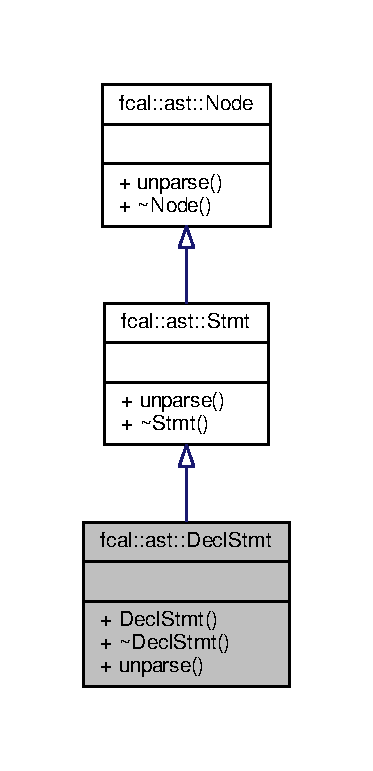
\includegraphics[width=179pt]{classfcal_1_1ast_1_1DeclStmt__inherit__graph}
\end{center}
\end{figure}


Collaboration diagram for fcal\+:\+:ast\+:\+:Decl\+Stmt\+:
\nopagebreak
\begin{figure}[H]
\begin{center}
\leavevmode
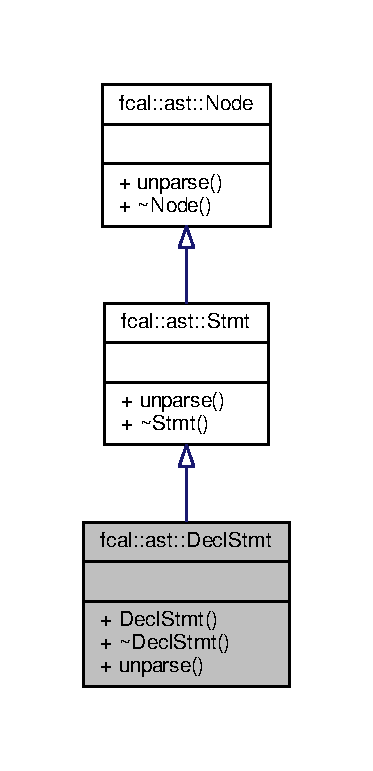
\includegraphics[width=179pt]{classfcal_1_1ast_1_1DeclStmt__coll__graph}
\end{center}
\end{figure}
\subsection*{Public Member Functions}
\begin{DoxyCompactItemize}
\item 
\hyperlink{classfcal_1_1ast_1_1DeclStmt_a5e958867a6deda40d828b0416406485b}{Decl\+Stmt} (\hyperlink{classfcal_1_1ast_1_1Decl}{Decl} $\ast$d)
\item 
\hyperlink{classfcal_1_1ast_1_1DeclStmt_ae9dfa80c23f0dd282556a7edf608fde9}{$\sim$\+Decl\+Stmt} ()
\item 
std\+::string \hyperlink{classfcal_1_1ast_1_1DeclStmt_a8c353eab134e5c531d4df740d48b6c06}{unparse} ()
\end{DoxyCompactItemize}


\subsection{Detailed Description}
The following classes directly inherit from the virtual \hyperlink{classfcal_1_1ast_1_1Stmt}{Stmt} class. These classes are used to construct the individual statements defined in the F\+C\+AL grammar. 

\subsection{Constructor \& Destructor Documentation}
\index{fcal\+::ast\+::\+Decl\+Stmt@{fcal\+::ast\+::\+Decl\+Stmt}!Decl\+Stmt@{Decl\+Stmt}}
\index{Decl\+Stmt@{Decl\+Stmt}!fcal\+::ast\+::\+Decl\+Stmt@{fcal\+::ast\+::\+Decl\+Stmt}}
\subsubsection[{\texorpdfstring{Decl\+Stmt(\+Decl $\ast$d)}{DeclStmt(Decl *d)}}]{\setlength{\rightskip}{0pt plus 5cm}fcal\+::ast\+::\+Decl\+Stmt\+::\+Decl\+Stmt (
\begin{DoxyParamCaption}
\item[{{\bf Decl} $\ast$}]{d}
\end{DoxyParamCaption}
)\hspace{0.3cm}{\ttfamily [inline]}, {\ttfamily [explicit]}}\hypertarget{classfcal_1_1ast_1_1DeclStmt_a5e958867a6deda40d828b0416406485b}{}\label{classfcal_1_1ast_1_1DeclStmt_a5e958867a6deda40d828b0416406485b}
\index{fcal\+::ast\+::\+Decl\+Stmt@{fcal\+::ast\+::\+Decl\+Stmt}!````~Decl\+Stmt@{$\sim$\+Decl\+Stmt}}
\index{````~Decl\+Stmt@{$\sim$\+Decl\+Stmt}!fcal\+::ast\+::\+Decl\+Stmt@{fcal\+::ast\+::\+Decl\+Stmt}}
\subsubsection[{\texorpdfstring{$\sim$\+Decl\+Stmt()}{~DeclStmt()}}]{\setlength{\rightskip}{0pt plus 5cm}fcal\+::ast\+::\+Decl\+Stmt\+::$\sim$\+Decl\+Stmt (
\begin{DoxyParamCaption}
{}
\end{DoxyParamCaption}
)\hspace{0.3cm}{\ttfamily [inline]}}\hypertarget{classfcal_1_1ast_1_1DeclStmt_ae9dfa80c23f0dd282556a7edf608fde9}{}\label{classfcal_1_1ast_1_1DeclStmt_ae9dfa80c23f0dd282556a7edf608fde9}


\subsection{Member Function Documentation}
\index{fcal\+::ast\+::\+Decl\+Stmt@{fcal\+::ast\+::\+Decl\+Stmt}!unparse@{unparse}}
\index{unparse@{unparse}!fcal\+::ast\+::\+Decl\+Stmt@{fcal\+::ast\+::\+Decl\+Stmt}}
\subsubsection[{\texorpdfstring{unparse()}{unparse()}}]{\setlength{\rightskip}{0pt plus 5cm}std\+::string fcal\+::ast\+::\+Decl\+Stmt\+::unparse (
\begin{DoxyParamCaption}
{}
\end{DoxyParamCaption}
)\hspace{0.3cm}{\ttfamily [inline]}, {\ttfamily [virtual]}}\hypertarget{classfcal_1_1ast_1_1DeclStmt_a8c353eab134e5c531d4df740d48b6c06}{}\label{classfcal_1_1ast_1_1DeclStmt_a8c353eab134e5c531d4df740d48b6c06}


Implements \hyperlink{classfcal_1_1ast_1_1Stmt_a2ed8595941ddc947012bfeae54f4447d}{fcal\+::ast\+::\+Stmt}.



The documentation for this class was generated from the following file\+:\begin{DoxyCompactItemize}
\item 
include/\hyperlink{ast_8h}{ast.\+h}\end{DoxyCompactItemize}

\hypertarget{classfcal_1_1ast_1_1DivideExpr}{}\section{fcal\+:\+:ast\+:\+:Divide\+Expr Class Reference}
\label{classfcal_1_1ast_1_1DivideExpr}\index{fcal\+::ast\+::\+Divide\+Expr@{fcal\+::ast\+::\+Divide\+Expr}}


{\ttfamily \#include $<$ast.\+h$>$}



Inheritance diagram for fcal\+:\+:ast\+:\+:Divide\+Expr\+:
\nopagebreak
\begin{figure}[H]
\begin{center}
\leavevmode
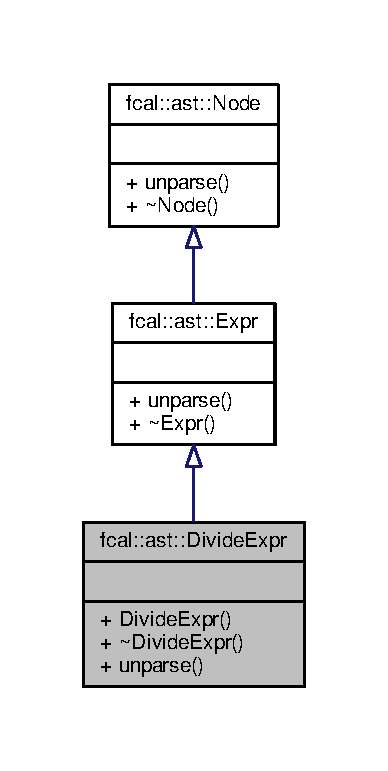
\includegraphics[width=186pt]{classfcal_1_1ast_1_1DivideExpr__inherit__graph}
\end{center}
\end{figure}


Collaboration diagram for fcal\+:\+:ast\+:\+:Divide\+Expr\+:
\nopagebreak
\begin{figure}[H]
\begin{center}
\leavevmode
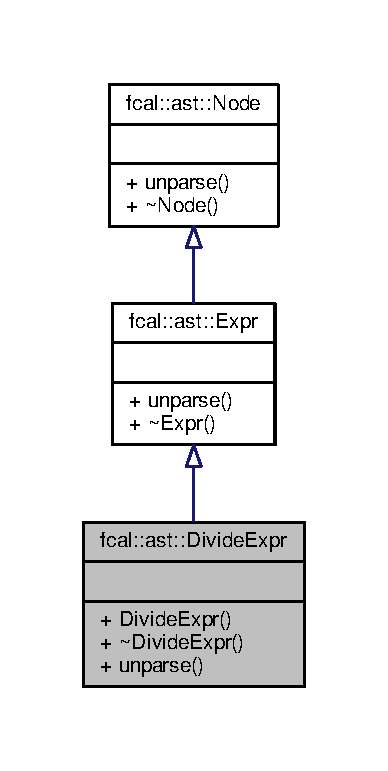
\includegraphics[width=186pt]{classfcal_1_1ast_1_1DivideExpr__coll__graph}
\end{center}
\end{figure}
\subsection*{Public Member Functions}
\begin{DoxyCompactItemize}
\item 
\hyperlink{classfcal_1_1ast_1_1DivideExpr_aedb4be7c3db38ae966d4a71765edaf85}{Divide\+Expr} (\hyperlink{classfcal_1_1ast_1_1Expr}{Expr} $\ast$e1, \hyperlink{classfcal_1_1ast_1_1Expr}{Expr} $\ast$e2)
\item 
\hyperlink{classfcal_1_1ast_1_1DivideExpr_a8a6e2087688a3570b9e3e7b1aaba93ef}{$\sim$\+Divide\+Expr} ()
\item 
std\+::string \hyperlink{classfcal_1_1ast_1_1DivideExpr_aa9ffeb0bd5a526ca75deacc31882f833}{unparse} ()
\end{DoxyCompactItemize}


\subsection{Constructor \& Destructor Documentation}
\index{fcal\+::ast\+::\+Divide\+Expr@{fcal\+::ast\+::\+Divide\+Expr}!Divide\+Expr@{Divide\+Expr}}
\index{Divide\+Expr@{Divide\+Expr}!fcal\+::ast\+::\+Divide\+Expr@{fcal\+::ast\+::\+Divide\+Expr}}
\subsubsection[{\texorpdfstring{Divide\+Expr(\+Expr $\ast$e1, Expr $\ast$e2)}{DivideExpr(Expr *e1, Expr *e2)}}]{\setlength{\rightskip}{0pt plus 5cm}fcal\+::ast\+::\+Divide\+Expr\+::\+Divide\+Expr (
\begin{DoxyParamCaption}
\item[{{\bf Expr} $\ast$}]{e1, }
\item[{{\bf Expr} $\ast$}]{e2}
\end{DoxyParamCaption}
)\hspace{0.3cm}{\ttfamily [inline]}}\hypertarget{classfcal_1_1ast_1_1DivideExpr_aedb4be7c3db38ae966d4a71765edaf85}{}\label{classfcal_1_1ast_1_1DivideExpr_aedb4be7c3db38ae966d4a71765edaf85}
\index{fcal\+::ast\+::\+Divide\+Expr@{fcal\+::ast\+::\+Divide\+Expr}!````~Divide\+Expr@{$\sim$\+Divide\+Expr}}
\index{````~Divide\+Expr@{$\sim$\+Divide\+Expr}!fcal\+::ast\+::\+Divide\+Expr@{fcal\+::ast\+::\+Divide\+Expr}}
\subsubsection[{\texorpdfstring{$\sim$\+Divide\+Expr()}{~DivideExpr()}}]{\setlength{\rightskip}{0pt plus 5cm}fcal\+::ast\+::\+Divide\+Expr\+::$\sim$\+Divide\+Expr (
\begin{DoxyParamCaption}
{}
\end{DoxyParamCaption}
)\hspace{0.3cm}{\ttfamily [inline]}}\hypertarget{classfcal_1_1ast_1_1DivideExpr_a8a6e2087688a3570b9e3e7b1aaba93ef}{}\label{classfcal_1_1ast_1_1DivideExpr_a8a6e2087688a3570b9e3e7b1aaba93ef}


\subsection{Member Function Documentation}
\index{fcal\+::ast\+::\+Divide\+Expr@{fcal\+::ast\+::\+Divide\+Expr}!unparse@{unparse}}
\index{unparse@{unparse}!fcal\+::ast\+::\+Divide\+Expr@{fcal\+::ast\+::\+Divide\+Expr}}
\subsubsection[{\texorpdfstring{unparse()}{unparse()}}]{\setlength{\rightskip}{0pt plus 5cm}std\+::string fcal\+::ast\+::\+Divide\+Expr\+::unparse (
\begin{DoxyParamCaption}
{}
\end{DoxyParamCaption}
)\hspace{0.3cm}{\ttfamily [inline]}, {\ttfamily [virtual]}}\hypertarget{classfcal_1_1ast_1_1DivideExpr_aa9ffeb0bd5a526ca75deacc31882f833}{}\label{classfcal_1_1ast_1_1DivideExpr_aa9ffeb0bd5a526ca75deacc31882f833}


Implements \hyperlink{classfcal_1_1ast_1_1Expr_adba9309749d00e7c864456fbd505f252}{fcal\+::ast\+::\+Expr}.



The documentation for this class was generated from the following file\+:\begin{DoxyCompactItemize}
\item 
include/\hyperlink{ast_8h}{ast.\+h}\end{DoxyCompactItemize}

\hypertarget{classfcal_1_1ast_1_1EmptyStmts}{}\section{fcal\+:\+:ast\+:\+:Empty\+Stmts Class Reference}
\label{classfcal_1_1ast_1_1EmptyStmts}\index{fcal\+::ast\+::\+Empty\+Stmts@{fcal\+::ast\+::\+Empty\+Stmts}}


{\ttfamily \#include $<$ast.\+h$>$}



Inheritance diagram for fcal\+:\+:ast\+:\+:Empty\+Stmts\+:
\nopagebreak
\begin{figure}[H]
\begin{center}
\leavevmode
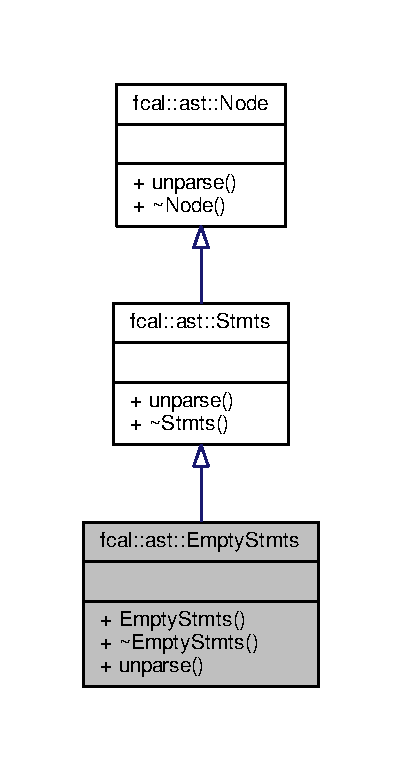
\includegraphics[width=193pt]{classfcal_1_1ast_1_1EmptyStmts__inherit__graph}
\end{center}
\end{figure}


Collaboration diagram for fcal\+:\+:ast\+:\+:Empty\+Stmts\+:
\nopagebreak
\begin{figure}[H]
\begin{center}
\leavevmode
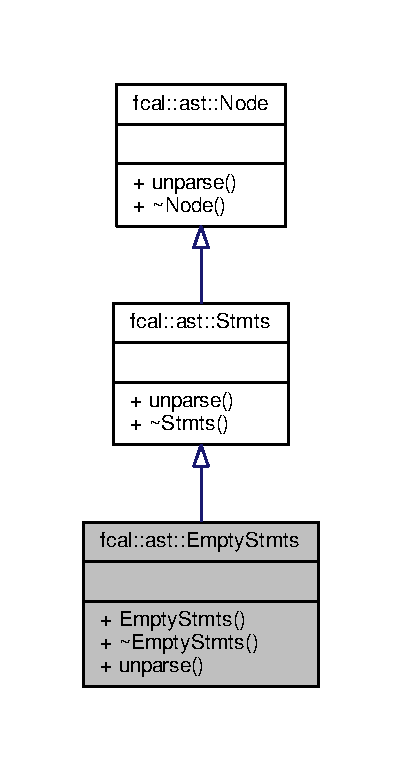
\includegraphics[width=193pt]{classfcal_1_1ast_1_1EmptyStmts__coll__graph}
\end{center}
\end{figure}
\subsection*{Public Member Functions}
\begin{DoxyCompactItemize}
\item 
\hyperlink{classfcal_1_1ast_1_1EmptyStmts_a3fffb31d194ba39a3f7cb22a75dba005}{Empty\+Stmts} ()
\item 
\hyperlink{classfcal_1_1ast_1_1EmptyStmts_ae477efcd74ff22bbacd04182658ce411}{$\sim$\+Empty\+Stmts} ()
\item 
std\+::string \hyperlink{classfcal_1_1ast_1_1EmptyStmts_abbccd9fb3e02082962774479fc47116d}{unparse} ()
\end{DoxyCompactItemize}


\subsection{Detailed Description}
The following classes directly inherit from the \hyperlink{classfcal_1_1ast_1_1Stmts}{Stmts} virtual class. These classes offer means to deconstruct sequences of individual statements as defined in the F\+C\+AL grammar. 

\subsection{Constructor \& Destructor Documentation}
\index{fcal\+::ast\+::\+Empty\+Stmts@{fcal\+::ast\+::\+Empty\+Stmts}!Empty\+Stmts@{Empty\+Stmts}}
\index{Empty\+Stmts@{Empty\+Stmts}!fcal\+::ast\+::\+Empty\+Stmts@{fcal\+::ast\+::\+Empty\+Stmts}}
\subsubsection[{\texorpdfstring{Empty\+Stmts()}{EmptyStmts()}}]{\setlength{\rightskip}{0pt plus 5cm}fcal\+::ast\+::\+Empty\+Stmts\+::\+Empty\+Stmts (
\begin{DoxyParamCaption}
{}
\end{DoxyParamCaption}
)\hspace{0.3cm}{\ttfamily [inline]}}\hypertarget{classfcal_1_1ast_1_1EmptyStmts_a3fffb31d194ba39a3f7cb22a75dba005}{}\label{classfcal_1_1ast_1_1EmptyStmts_a3fffb31d194ba39a3f7cb22a75dba005}
\index{fcal\+::ast\+::\+Empty\+Stmts@{fcal\+::ast\+::\+Empty\+Stmts}!````~Empty\+Stmts@{$\sim$\+Empty\+Stmts}}
\index{````~Empty\+Stmts@{$\sim$\+Empty\+Stmts}!fcal\+::ast\+::\+Empty\+Stmts@{fcal\+::ast\+::\+Empty\+Stmts}}
\subsubsection[{\texorpdfstring{$\sim$\+Empty\+Stmts()}{~EmptyStmts()}}]{\setlength{\rightskip}{0pt plus 5cm}fcal\+::ast\+::\+Empty\+Stmts\+::$\sim$\+Empty\+Stmts (
\begin{DoxyParamCaption}
{}
\end{DoxyParamCaption}
)\hspace{0.3cm}{\ttfamily [inline]}}\hypertarget{classfcal_1_1ast_1_1EmptyStmts_ae477efcd74ff22bbacd04182658ce411}{}\label{classfcal_1_1ast_1_1EmptyStmts_ae477efcd74ff22bbacd04182658ce411}


\subsection{Member Function Documentation}
\index{fcal\+::ast\+::\+Empty\+Stmts@{fcal\+::ast\+::\+Empty\+Stmts}!unparse@{unparse}}
\index{unparse@{unparse}!fcal\+::ast\+::\+Empty\+Stmts@{fcal\+::ast\+::\+Empty\+Stmts}}
\subsubsection[{\texorpdfstring{unparse()}{unparse()}}]{\setlength{\rightskip}{0pt plus 5cm}std\+::string fcal\+::ast\+::\+Empty\+Stmts\+::unparse (
\begin{DoxyParamCaption}
{}
\end{DoxyParamCaption}
)\hspace{0.3cm}{\ttfamily [inline]}, {\ttfamily [virtual]}}\hypertarget{classfcal_1_1ast_1_1EmptyStmts_abbccd9fb3e02082962774479fc47116d}{}\label{classfcal_1_1ast_1_1EmptyStmts_abbccd9fb3e02082962774479fc47116d}


Implements \hyperlink{classfcal_1_1ast_1_1Stmts_a1a01ed57e1a564a482ed11caf0e813df}{fcal\+::ast\+::\+Stmts}.



The documentation for this class was generated from the following file\+:\begin{DoxyCompactItemize}
\item 
include/\hyperlink{ast_8h}{ast.\+h}\end{DoxyCompactItemize}

\hypertarget{classfcal_1_1scanner_1_1EndOfFileToken}{}\section{fcal\+:\+:scanner\+:\+:End\+Of\+File\+Token Class Reference}
\label{classfcal_1_1scanner_1_1EndOfFileToken}\index{fcal\+::scanner\+::\+End\+Of\+File\+Token@{fcal\+::scanner\+::\+End\+Of\+File\+Token}}


{\ttfamily \#include $<$ext\+\_\+token.\+h$>$}



Inheritance diagram for fcal\+:\+:scanner\+:\+:End\+Of\+File\+Token\+:
\nopagebreak
\begin{figure}[H]
\begin{center}
\leavevmode
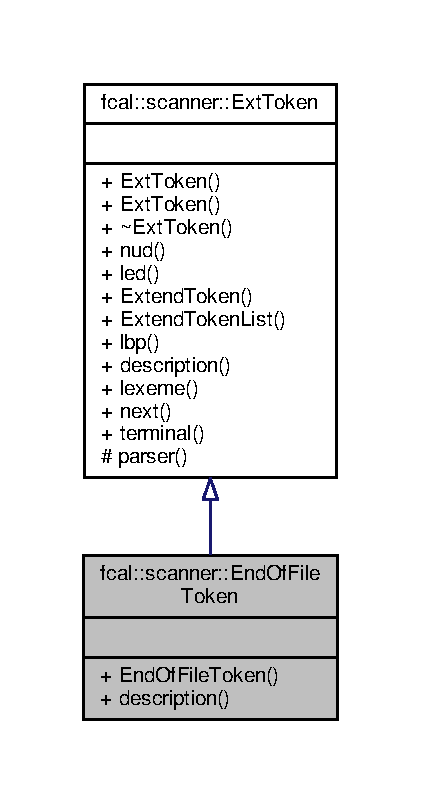
\includegraphics[width=202pt]{classfcal_1_1scanner_1_1EndOfFileToken__inherit__graph}
\end{center}
\end{figure}


Collaboration diagram for fcal\+:\+:scanner\+:\+:End\+Of\+File\+Token\+:
\nopagebreak
\begin{figure}[H]
\begin{center}
\leavevmode
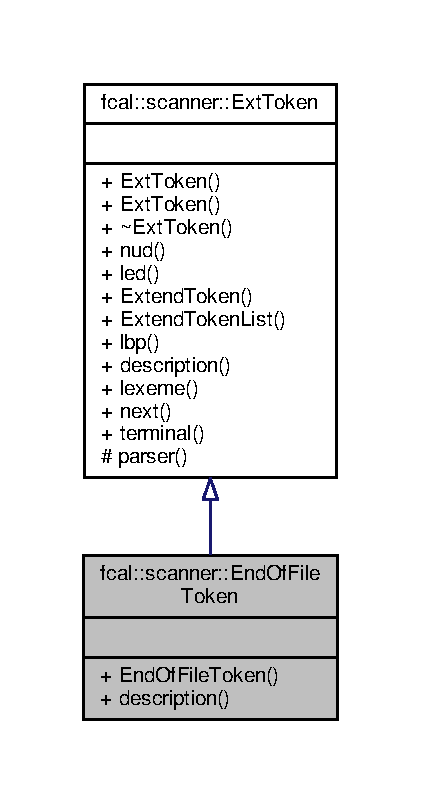
\includegraphics[width=202pt]{classfcal_1_1scanner_1_1EndOfFileToken__coll__graph}
\end{center}
\end{figure}
\subsection*{Public Member Functions}
\begin{DoxyCompactItemize}
\item 
\hyperlink{classfcal_1_1scanner_1_1EndOfFileToken_a275106595ca3f5a46c80efb281021f2b}{End\+Of\+File\+Token} (\hyperlink{classfcal_1_1parser_1_1Parser}{parser\+::\+Parser} $\ast$p, \hyperlink{classfcal_1_1scanner_1_1Token}{Token} $\ast$t)
\item 
std\+::string \hyperlink{classfcal_1_1scanner_1_1EndOfFileToken_a8fdfe21df812622405e5b7814970f367}{description} ()
\end{DoxyCompactItemize}
\subsection*{Additional Inherited Members}


\subsection{Constructor \& Destructor Documentation}
\index{fcal\+::scanner\+::\+End\+Of\+File\+Token@{fcal\+::scanner\+::\+End\+Of\+File\+Token}!End\+Of\+File\+Token@{End\+Of\+File\+Token}}
\index{End\+Of\+File\+Token@{End\+Of\+File\+Token}!fcal\+::scanner\+::\+End\+Of\+File\+Token@{fcal\+::scanner\+::\+End\+Of\+File\+Token}}
\subsubsection[{\texorpdfstring{End\+Of\+File\+Token(parser\+::\+Parser $\ast$p, Token $\ast$t)}{EndOfFileToken(parser::Parser *p, Token *t)}}]{\setlength{\rightskip}{0pt plus 5cm}fcal\+::scanner\+::\+End\+Of\+File\+Token\+::\+End\+Of\+File\+Token (
\begin{DoxyParamCaption}
\item[{{\bf parser\+::\+Parser} $\ast$}]{p, }
\item[{{\bf Token} $\ast$}]{t}
\end{DoxyParamCaption}
)\hspace{0.3cm}{\ttfamily [inline]}}\hypertarget{classfcal_1_1scanner_1_1EndOfFileToken_a275106595ca3f5a46c80efb281021f2b}{}\label{classfcal_1_1scanner_1_1EndOfFileToken_a275106595ca3f5a46c80efb281021f2b}


\subsection{Member Function Documentation}
\index{fcal\+::scanner\+::\+End\+Of\+File\+Token@{fcal\+::scanner\+::\+End\+Of\+File\+Token}!description@{description}}
\index{description@{description}!fcal\+::scanner\+::\+End\+Of\+File\+Token@{fcal\+::scanner\+::\+End\+Of\+File\+Token}}
\subsubsection[{\texorpdfstring{description()}{description()}}]{\setlength{\rightskip}{0pt plus 5cm}std\+::string fcal\+::scanner\+::\+End\+Of\+File\+Token\+::description (
\begin{DoxyParamCaption}
{}
\end{DoxyParamCaption}
)\hspace{0.3cm}{\ttfamily [inline]}, {\ttfamily [virtual]}}\hypertarget{classfcal_1_1scanner_1_1EndOfFileToken_a8fdfe21df812622405e5b7814970f367}{}\label{classfcal_1_1scanner_1_1EndOfFileToken_a8fdfe21df812622405e5b7814970f367}


Reimplemented from \hyperlink{classfcal_1_1scanner_1_1ExtToken_a29a72149492d7fef7968a1b894d334c7}{fcal\+::scanner\+::\+Ext\+Token}.



The documentation for this class was generated from the following file\+:\begin{DoxyCompactItemize}
\item 
include/\hyperlink{ext__token_8h}{ext\+\_\+token.\+h}\end{DoxyCompactItemize}

\hypertarget{classfcal_1_1ast_1_1EqualsEqualsExpr}{}\section{fcal\+:\+:ast\+:\+:Equals\+Equals\+Expr Class Reference}
\label{classfcal_1_1ast_1_1EqualsEqualsExpr}\index{fcal\+::ast\+::\+Equals\+Equals\+Expr@{fcal\+::ast\+::\+Equals\+Equals\+Expr}}


{\ttfamily \#include $<$ast.\+h$>$}



Inheritance diagram for fcal\+:\+:ast\+:\+:Equals\+Equals\+Expr\+:
\nopagebreak
\begin{figure}[H]
\begin{center}
\leavevmode
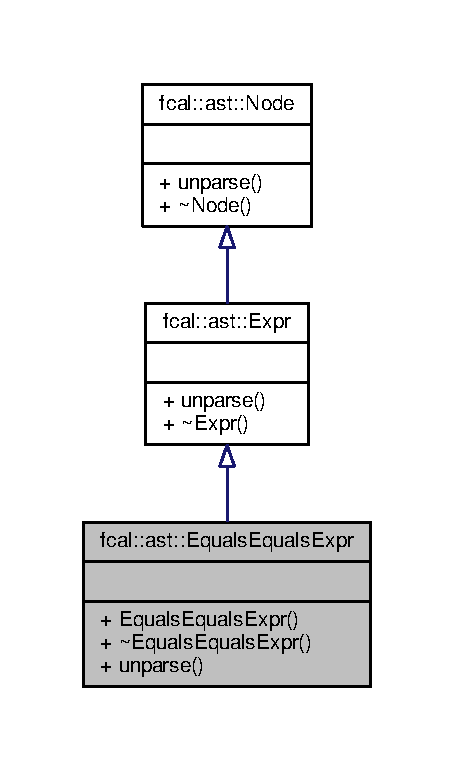
\includegraphics[width=218pt]{classfcal_1_1ast_1_1EqualsEqualsExpr__inherit__graph}
\end{center}
\end{figure}


Collaboration diagram for fcal\+:\+:ast\+:\+:Equals\+Equals\+Expr\+:
\nopagebreak
\begin{figure}[H]
\begin{center}
\leavevmode
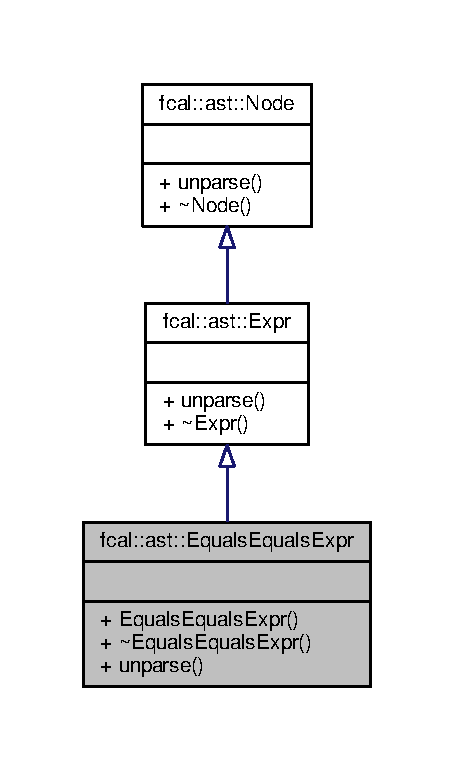
\includegraphics[width=218pt]{classfcal_1_1ast_1_1EqualsEqualsExpr__coll__graph}
\end{center}
\end{figure}
\subsection*{Public Member Functions}
\begin{DoxyCompactItemize}
\item 
\hyperlink{classfcal_1_1ast_1_1EqualsEqualsExpr_a2b3efec176a7c9748a7992b0212fd489}{Equals\+Equals\+Expr} (\hyperlink{classfcal_1_1ast_1_1Expr}{Expr} $\ast$e1, \hyperlink{classfcal_1_1ast_1_1Expr}{Expr} $\ast$e2)
\item 
\hyperlink{classfcal_1_1ast_1_1EqualsEqualsExpr_a5c325abf38775a8d4ce8b7176fb3f69e}{$\sim$\+Equals\+Equals\+Expr} ()
\item 
std\+::string \hyperlink{classfcal_1_1ast_1_1EqualsEqualsExpr_a48f3a989601a76e3de580be1d84c7eeb}{unparse} ()
\end{DoxyCompactItemize}


\subsection{Constructor \& Destructor Documentation}
\index{fcal\+::ast\+::\+Equals\+Equals\+Expr@{fcal\+::ast\+::\+Equals\+Equals\+Expr}!Equals\+Equals\+Expr@{Equals\+Equals\+Expr}}
\index{Equals\+Equals\+Expr@{Equals\+Equals\+Expr}!fcal\+::ast\+::\+Equals\+Equals\+Expr@{fcal\+::ast\+::\+Equals\+Equals\+Expr}}
\subsubsection[{\texorpdfstring{Equals\+Equals\+Expr(\+Expr $\ast$e1, Expr $\ast$e2)}{EqualsEqualsExpr(Expr *e1, Expr *e2)}}]{\setlength{\rightskip}{0pt plus 5cm}fcal\+::ast\+::\+Equals\+Equals\+Expr\+::\+Equals\+Equals\+Expr (
\begin{DoxyParamCaption}
\item[{{\bf Expr} $\ast$}]{e1, }
\item[{{\bf Expr} $\ast$}]{e2}
\end{DoxyParamCaption}
)\hspace{0.3cm}{\ttfamily [inline]}}\hypertarget{classfcal_1_1ast_1_1EqualsEqualsExpr_a2b3efec176a7c9748a7992b0212fd489}{}\label{classfcal_1_1ast_1_1EqualsEqualsExpr_a2b3efec176a7c9748a7992b0212fd489}
\index{fcal\+::ast\+::\+Equals\+Equals\+Expr@{fcal\+::ast\+::\+Equals\+Equals\+Expr}!````~Equals\+Equals\+Expr@{$\sim$\+Equals\+Equals\+Expr}}
\index{````~Equals\+Equals\+Expr@{$\sim$\+Equals\+Equals\+Expr}!fcal\+::ast\+::\+Equals\+Equals\+Expr@{fcal\+::ast\+::\+Equals\+Equals\+Expr}}
\subsubsection[{\texorpdfstring{$\sim$\+Equals\+Equals\+Expr()}{~EqualsEqualsExpr()}}]{\setlength{\rightskip}{0pt plus 5cm}fcal\+::ast\+::\+Equals\+Equals\+Expr\+::$\sim$\+Equals\+Equals\+Expr (
\begin{DoxyParamCaption}
{}
\end{DoxyParamCaption}
)\hspace{0.3cm}{\ttfamily [inline]}}\hypertarget{classfcal_1_1ast_1_1EqualsEqualsExpr_a5c325abf38775a8d4ce8b7176fb3f69e}{}\label{classfcal_1_1ast_1_1EqualsEqualsExpr_a5c325abf38775a8d4ce8b7176fb3f69e}


\subsection{Member Function Documentation}
\index{fcal\+::ast\+::\+Equals\+Equals\+Expr@{fcal\+::ast\+::\+Equals\+Equals\+Expr}!unparse@{unparse}}
\index{unparse@{unparse}!fcal\+::ast\+::\+Equals\+Equals\+Expr@{fcal\+::ast\+::\+Equals\+Equals\+Expr}}
\subsubsection[{\texorpdfstring{unparse()}{unparse()}}]{\setlength{\rightskip}{0pt plus 5cm}std\+::string fcal\+::ast\+::\+Equals\+Equals\+Expr\+::unparse (
\begin{DoxyParamCaption}
{}
\end{DoxyParamCaption}
)\hspace{0.3cm}{\ttfamily [inline]}, {\ttfamily [virtual]}}\hypertarget{classfcal_1_1ast_1_1EqualsEqualsExpr_a48f3a989601a76e3de580be1d84c7eeb}{}\label{classfcal_1_1ast_1_1EqualsEqualsExpr_a48f3a989601a76e3de580be1d84c7eeb}


Implements \hyperlink{classfcal_1_1ast_1_1Expr_adba9309749d00e7c864456fbd505f252}{fcal\+::ast\+::\+Expr}.



The documentation for this class was generated from the following file\+:\begin{DoxyCompactItemize}
\item 
include/\hyperlink{ast_8h}{ast.\+h}\end{DoxyCompactItemize}

\hypertarget{classfcal_1_1ast_1_1Expr}{}\section{fcal\+:\+:ast\+:\+:Expr Class Reference}
\label{classfcal_1_1ast_1_1Expr}\index{fcal\+::ast\+::\+Expr@{fcal\+::ast\+::\+Expr}}


{\ttfamily \#include $<$ast.\+h$>$}



Inheritance diagram for fcal\+:\+:ast\+:\+:Expr\+:
\nopagebreak
\begin{figure}[H]
\begin{center}
\leavevmode
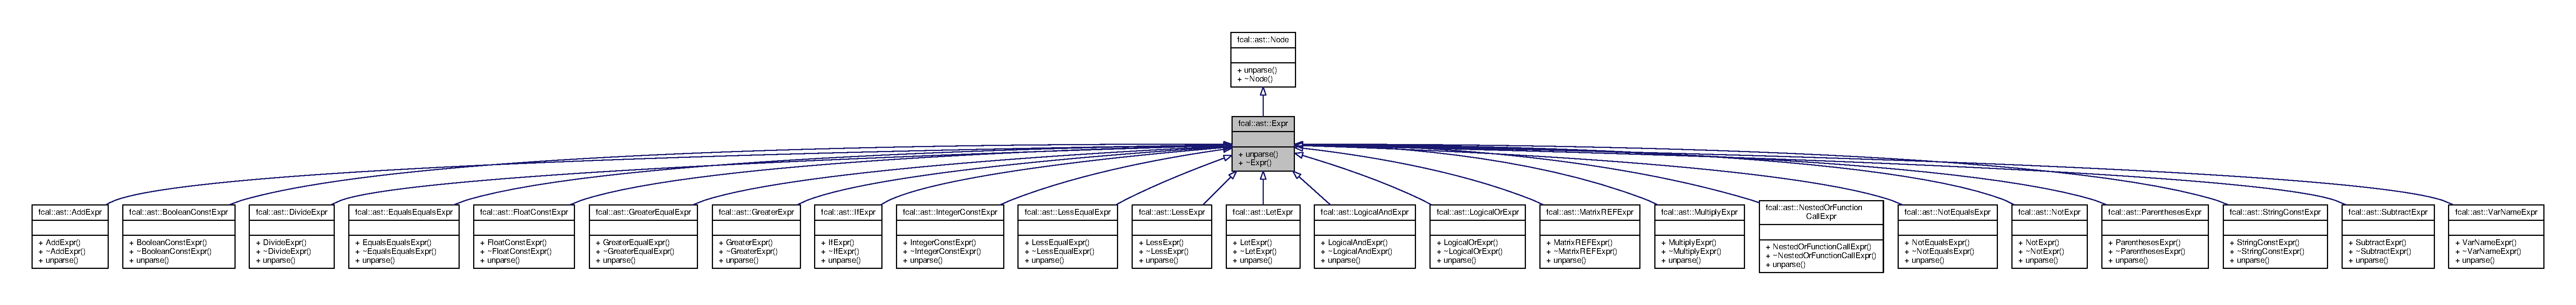
\includegraphics[width=350pt]{classfcal_1_1ast_1_1Expr__inherit__graph}
\end{center}
\end{figure}


Collaboration diagram for fcal\+:\+:ast\+:\+:Expr\+:
\nopagebreak
\begin{figure}[H]
\begin{center}
\leavevmode
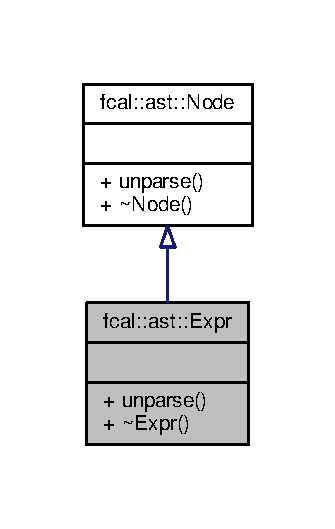
\includegraphics[width=161pt]{classfcal_1_1ast_1_1Expr__coll__graph}
\end{center}
\end{figure}
\subsection*{Public Member Functions}
\begin{DoxyCompactItemize}
\item 
virtual std\+::string \hyperlink{classfcal_1_1ast_1_1Expr_adba9309749d00e7c864456fbd505f252}{unparse} ()=0
\item 
virtual \hyperlink{classfcal_1_1ast_1_1Expr_a45a2b85849dc60f043f5d60b46fc1fcc}{$\sim$\+Expr} ()
\end{DoxyCompactItemize}


\subsection{Constructor \& Destructor Documentation}
\index{fcal\+::ast\+::\+Expr@{fcal\+::ast\+::\+Expr}!````~Expr@{$\sim$\+Expr}}
\index{````~Expr@{$\sim$\+Expr}!fcal\+::ast\+::\+Expr@{fcal\+::ast\+::\+Expr}}
\subsubsection[{\texorpdfstring{$\sim$\+Expr()}{~Expr()}}]{\setlength{\rightskip}{0pt plus 5cm}virtual fcal\+::ast\+::\+Expr\+::$\sim$\+Expr (
\begin{DoxyParamCaption}
{}
\end{DoxyParamCaption}
)\hspace{0.3cm}{\ttfamily [inline]}, {\ttfamily [virtual]}}\hypertarget{classfcal_1_1ast_1_1Expr_a45a2b85849dc60f043f5d60b46fc1fcc}{}\label{classfcal_1_1ast_1_1Expr_a45a2b85849dc60f043f5d60b46fc1fcc}


\subsection{Member Function Documentation}
\index{fcal\+::ast\+::\+Expr@{fcal\+::ast\+::\+Expr}!unparse@{unparse}}
\index{unparse@{unparse}!fcal\+::ast\+::\+Expr@{fcal\+::ast\+::\+Expr}}
\subsubsection[{\texorpdfstring{unparse()=0}{unparse()=0}}]{\setlength{\rightskip}{0pt plus 5cm}virtual std\+::string fcal\+::ast\+::\+Expr\+::unparse (
\begin{DoxyParamCaption}
{}
\end{DoxyParamCaption}
)\hspace{0.3cm}{\ttfamily [pure virtual]}}\hypertarget{classfcal_1_1ast_1_1Expr_adba9309749d00e7c864456fbd505f252}{}\label{classfcal_1_1ast_1_1Expr_adba9309749d00e7c864456fbd505f252}


Implements \hyperlink{classfcal_1_1ast_1_1Node_a81865f5a1df593708a39bf492952742a}{fcal\+::ast\+::\+Node}.



Implemented in \hyperlink{classfcal_1_1ast_1_1NotExpr_a46f164e673738d573c8616c70c26159f}{fcal\+::ast\+::\+Not\+Expr}, \hyperlink{classfcal_1_1ast_1_1IfExpr_a4092cf20150a2cde02364d4c7233e558}{fcal\+::ast\+::\+If\+Expr}, \hyperlink{classfcal_1_1ast_1_1LetExpr_a5277bbe3510e870f65dd9158592ef6da}{fcal\+::ast\+::\+Let\+Expr}, \hyperlink{classfcal_1_1ast_1_1ParenthesesExpr_aeeecf677f1f0e03771004cb611347732}{fcal\+::ast\+::\+Parentheses\+Expr}, \hyperlink{classfcal_1_1ast_1_1NestedOrFunctionCallExpr_aba7c47b3587c8d9e9c1d18e30f005c45}{fcal\+::ast\+::\+Nested\+Or\+Function\+Call\+Expr}, \hyperlink{classfcal_1_1ast_1_1MatrixREFExpr_a894e3996a1b1703dc767433df98b551f}{fcal\+::ast\+::\+Matrix\+R\+E\+F\+Expr}, \hyperlink{classfcal_1_1ast_1_1LogicalOrExpr_a0553c24537ac515e8f66ada8200a14c9}{fcal\+::ast\+::\+Logical\+Or\+Expr}, \hyperlink{classfcal_1_1ast_1_1LogicalAndExpr_ade9698171dd31ad7253f7e2a96a72a04}{fcal\+::ast\+::\+Logical\+And\+Expr}, \hyperlink{classfcal_1_1ast_1_1NotEqualsExpr_a6b00eebe998ad14fa56f52630f0d5bf9}{fcal\+::ast\+::\+Not\+Equals\+Expr}, \hyperlink{classfcal_1_1ast_1_1EqualsEqualsExpr_a48f3a989601a76e3de580be1d84c7eeb}{fcal\+::ast\+::\+Equals\+Equals\+Expr}, \hyperlink{classfcal_1_1ast_1_1LessEqualExpr_a78181c2bc69a185d97753d23c823b6a0}{fcal\+::ast\+::\+Less\+Equal\+Expr}, \hyperlink{classfcal_1_1ast_1_1LessExpr_af3a7eb1f384374183b28ca01224827e2}{fcal\+::ast\+::\+Less\+Expr}, \hyperlink{classfcal_1_1ast_1_1GreaterEqualExpr_a1ae9a0851f31b4740ffb8a35a9014478}{fcal\+::ast\+::\+Greater\+Equal\+Expr}, \hyperlink{classfcal_1_1ast_1_1GreaterExpr_ad5bd1acf689d89841845e14d63e42e16}{fcal\+::ast\+::\+Greater\+Expr}, \hyperlink{classfcal_1_1ast_1_1SubtractExpr_af9743e29d8e72ee1a33a55470cad923e}{fcal\+::ast\+::\+Subtract\+Expr}, \hyperlink{classfcal_1_1ast_1_1AddExpr_ab091a379ec85a4f0d3861f440d3fb54e}{fcal\+::ast\+::\+Add\+Expr}, \hyperlink{classfcal_1_1ast_1_1DivideExpr_aa9ffeb0bd5a526ca75deacc31882f833}{fcal\+::ast\+::\+Divide\+Expr}, \hyperlink{classfcal_1_1ast_1_1MultiplyExpr_a95d9a65fb0f15fea8d94156f64979ca3}{fcal\+::ast\+::\+Multiply\+Expr}, \hyperlink{classfcal_1_1ast_1_1BooleanConstExpr_a24fbd101f0aa59fc7379b2365f4f84be}{fcal\+::ast\+::\+Boolean\+Const\+Expr}, \hyperlink{classfcal_1_1ast_1_1StringConstExpr_a31ebd91190d48077a842cd711c5b0f26}{fcal\+::ast\+::\+String\+Const\+Expr}, \hyperlink{classfcal_1_1ast_1_1FloatConstExpr_ac43f676dc814852231c0ac263d1a2628}{fcal\+::ast\+::\+Float\+Const\+Expr}, \hyperlink{classfcal_1_1ast_1_1IntegerConstExpr_afccb833ff588cd49929358ab76cafdc4}{fcal\+::ast\+::\+Integer\+Const\+Expr}, and \hyperlink{classfcal_1_1ast_1_1VarNameExpr_a07df9e3944650d2d2495d68af50dae0c}{fcal\+::ast\+::\+Var\+Name\+Expr}.



The documentation for this class was generated from the following file\+:\begin{DoxyCompactItemize}
\item 
include/\hyperlink{ast_8h}{ast.\+h}\end{DoxyCompactItemize}

\hypertarget{classfcal_1_1scanner_1_1ExtToken}{}\section{fcal\+:\+:scanner\+:\+:Ext\+Token Class Reference}
\label{classfcal_1_1scanner_1_1ExtToken}\index{fcal\+::scanner\+::\+Ext\+Token@{fcal\+::scanner\+::\+Ext\+Token}}


{\ttfamily \#include $<$ext\+\_\+token.\+h$>$}



Inheritance diagram for fcal\+:\+:scanner\+:\+:Ext\+Token\+:
\nopagebreak
\begin{figure}[H]
\begin{center}
\leavevmode
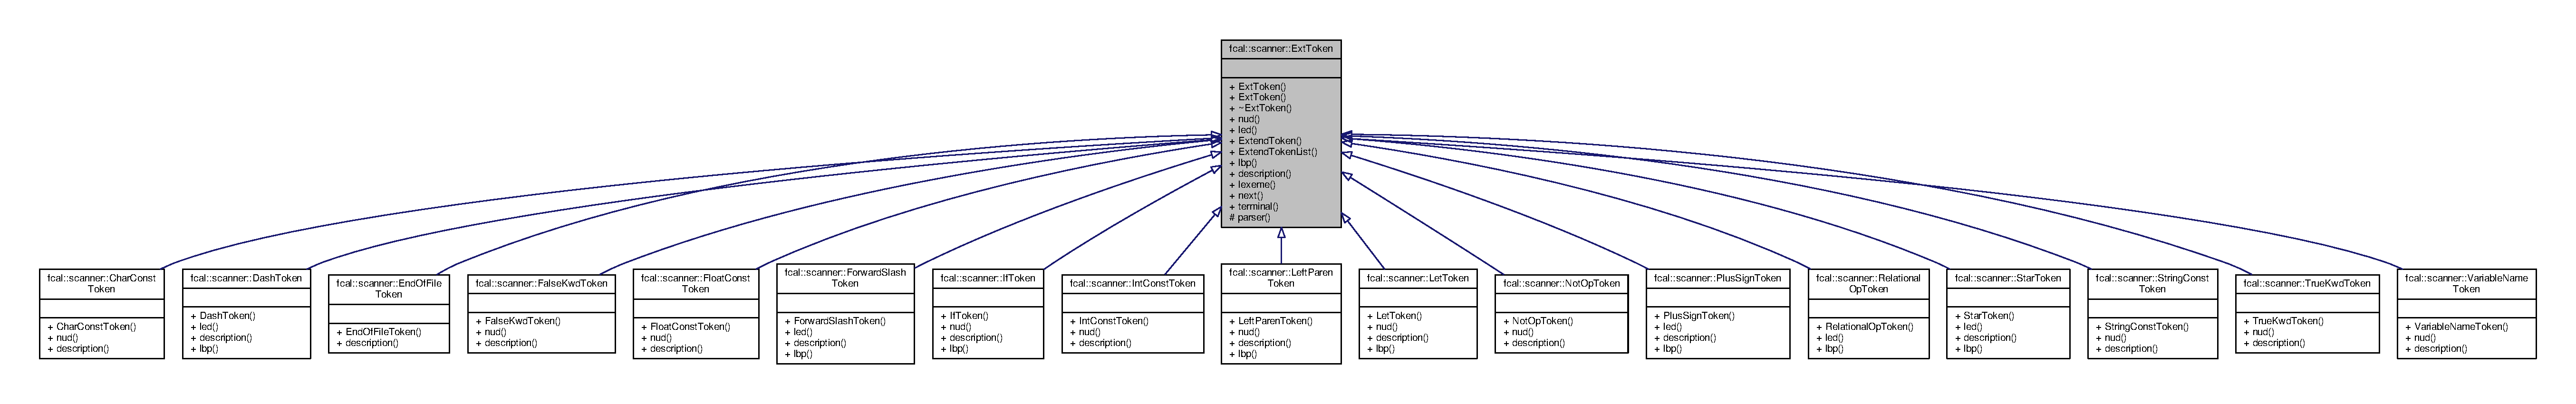
\includegraphics[width=350pt]{classfcal_1_1scanner_1_1ExtToken__inherit__graph}
\end{center}
\end{figure}


Collaboration diagram for fcal\+:\+:scanner\+:\+:Ext\+Token\+:
\nopagebreak
\begin{figure}[H]
\begin{center}
\leavevmode
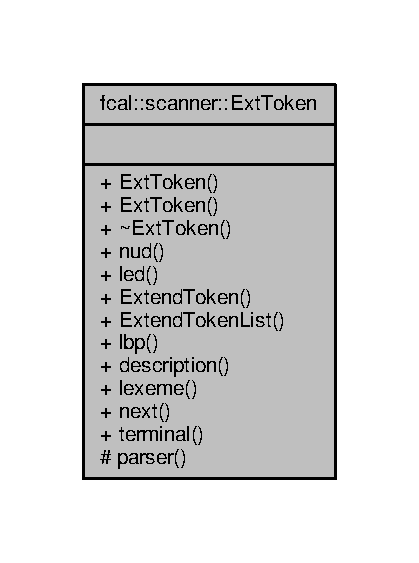
\includegraphics[width=201pt]{classfcal_1_1scanner_1_1ExtToken__coll__graph}
\end{center}
\end{figure}
\subsection*{Public Member Functions}
\begin{DoxyCompactItemize}
\item 
\hyperlink{classfcal_1_1scanner_1_1ExtToken_afda92e9d2c7b66f2b9aaed8ac07bca46}{Ext\+Token} (\hyperlink{classfcal_1_1parser_1_1Parser}{parser\+::\+Parser} $\ast$p, \hyperlink{classfcal_1_1scanner_1_1Token}{Token} $\ast$t)
\item 
\hyperlink{classfcal_1_1scanner_1_1ExtToken_aa6846c2c9fb91a37715b0f41a0ffcda4}{Ext\+Token} (\hyperlink{classfcal_1_1parser_1_1Parser}{parser\+::\+Parser} $\ast$p, \hyperlink{classfcal_1_1scanner_1_1Token}{Token} $\ast$t, std\+::string d)
\item 
virtual \hyperlink{classfcal_1_1scanner_1_1ExtToken_a13fe524a7fa31549acd6c5e8769d0a84}{$\sim$\+Ext\+Token} ()
\item 
virtual \hyperlink{classfcal_1_1parser_1_1ParseResult}{parser\+::\+Parse\+Result} \hyperlink{classfcal_1_1scanner_1_1ExtToken_a2e1ca27a07d55593ffd67780dbcad7dd}{nud} (void)
\item 
virtual \hyperlink{classfcal_1_1parser_1_1ParseResult}{parser\+::\+Parse\+Result} \hyperlink{classfcal_1_1scanner_1_1ExtToken_a42c352ef5e019a1155be80b4a40deb38}{led} (\hyperlink{classfcal_1_1parser_1_1ParseResult}{parser\+::\+Parse\+Result} left)
\item 
\hyperlink{classfcal_1_1scanner_1_1ExtToken}{Ext\+Token} $\ast$ \hyperlink{classfcal_1_1scanner_1_1ExtToken_ad6a5965961553c85d7fbaa688fabf052}{Extend\+Token} (\hyperlink{classfcal_1_1parser_1_1Parser}{parser\+::\+Parser} $\ast$p, \hyperlink{classfcal_1_1scanner_1_1Token}{Token} $\ast$tokens)
\item 
\hyperlink{classfcal_1_1scanner_1_1ExtToken}{Ext\+Token} $\ast$ \hyperlink{classfcal_1_1scanner_1_1ExtToken_a4995af1527ea8ba6ee99f3fa8646856d}{Extend\+Token\+List} (\hyperlink{classfcal_1_1parser_1_1Parser}{parser\+::\+Parser} $\ast$p, \hyperlink{classfcal_1_1scanner_1_1Token}{Token} $\ast$tokens)
\item 
virtual int \hyperlink{classfcal_1_1scanner_1_1ExtToken_adecef3770f08e5a26f103ab62171cc91}{lbp} ()
\item 
virtual std\+::string \hyperlink{classfcal_1_1scanner_1_1ExtToken_a29a72149492d7fef7968a1b894d334c7}{description} ()
\item 
std\+::string \hyperlink{classfcal_1_1scanner_1_1ExtToken_a32d06bece581a1711625c3a503db21e1}{lexeme} (void) const 
\item 
\hyperlink{classfcal_1_1scanner_1_1ExtToken}{Ext\+Token} $\ast$ \hyperlink{classfcal_1_1scanner_1_1ExtToken_aa927cdbdee70b7e74e0aee075f340472}{next} (void) const 
\item 
\hyperlink{namespacefcal_1_1scanner_ad95bd8241e3350b2d765f6b929eb0d93}{scanner\+::\+Token\+Type} \hyperlink{classfcal_1_1scanner_1_1ExtToken_a0bc057f41ebfeab0900a467af3798bbf}{terminal} (void) const 
\end{DoxyCompactItemize}
\subsection*{Protected Member Functions}
\begin{DoxyCompactItemize}
\item 
\hyperlink{classfcal_1_1parser_1_1Parser}{parser\+::\+Parser} $\ast$ \hyperlink{classfcal_1_1scanner_1_1ExtToken_a311bc29b9732fc7825012ecf08d1d73f}{parser} (void)
\end{DoxyCompactItemize}


\subsection{Constructor \& Destructor Documentation}
\index{fcal\+::scanner\+::\+Ext\+Token@{fcal\+::scanner\+::\+Ext\+Token}!Ext\+Token@{Ext\+Token}}
\index{Ext\+Token@{Ext\+Token}!fcal\+::scanner\+::\+Ext\+Token@{fcal\+::scanner\+::\+Ext\+Token}}
\subsubsection[{\texorpdfstring{Ext\+Token(parser\+::\+Parser $\ast$p, Token $\ast$t)}{ExtToken(parser::Parser *p, Token *t)}}]{\setlength{\rightskip}{0pt plus 5cm}fcal\+::scanner\+::\+Ext\+Token\+::\+Ext\+Token (
\begin{DoxyParamCaption}
\item[{{\bf parser\+::\+Parser} $\ast$}]{p, }
\item[{{\bf Token} $\ast$}]{t}
\end{DoxyParamCaption}
)\hspace{0.3cm}{\ttfamily [inline]}}\hypertarget{classfcal_1_1scanner_1_1ExtToken_afda92e9d2c7b66f2b9aaed8ac07bca46}{}\label{classfcal_1_1scanner_1_1ExtToken_afda92e9d2c7b66f2b9aaed8ac07bca46}
\index{fcal\+::scanner\+::\+Ext\+Token@{fcal\+::scanner\+::\+Ext\+Token}!Ext\+Token@{Ext\+Token}}
\index{Ext\+Token@{Ext\+Token}!fcal\+::scanner\+::\+Ext\+Token@{fcal\+::scanner\+::\+Ext\+Token}}
\subsubsection[{\texorpdfstring{Ext\+Token(parser\+::\+Parser $\ast$p, Token $\ast$t, std\+::string d)}{ExtToken(parser::Parser *p, Token *t, std::string d)}}]{\setlength{\rightskip}{0pt plus 5cm}fcal\+::scanner\+::\+Ext\+Token\+::\+Ext\+Token (
\begin{DoxyParamCaption}
\item[{{\bf parser\+::\+Parser} $\ast$}]{p, }
\item[{{\bf Token} $\ast$}]{t, }
\item[{std\+::string}]{d}
\end{DoxyParamCaption}
)\hspace{0.3cm}{\ttfamily [inline]}}\hypertarget{classfcal_1_1scanner_1_1ExtToken_aa6846c2c9fb91a37715b0f41a0ffcda4}{}\label{classfcal_1_1scanner_1_1ExtToken_aa6846c2c9fb91a37715b0f41a0ffcda4}
\index{fcal\+::scanner\+::\+Ext\+Token@{fcal\+::scanner\+::\+Ext\+Token}!````~Ext\+Token@{$\sim$\+Ext\+Token}}
\index{````~Ext\+Token@{$\sim$\+Ext\+Token}!fcal\+::scanner\+::\+Ext\+Token@{fcal\+::scanner\+::\+Ext\+Token}}
\subsubsection[{\texorpdfstring{$\sim$\+Ext\+Token()}{~ExtToken()}}]{\setlength{\rightskip}{0pt plus 5cm}virtual fcal\+::scanner\+::\+Ext\+Token\+::$\sim$\+Ext\+Token (
\begin{DoxyParamCaption}
{}
\end{DoxyParamCaption}
)\hspace{0.3cm}{\ttfamily [inline]}, {\ttfamily [virtual]}}\hypertarget{classfcal_1_1scanner_1_1ExtToken_a13fe524a7fa31549acd6c5e8769d0a84}{}\label{classfcal_1_1scanner_1_1ExtToken_a13fe524a7fa31549acd6c5e8769d0a84}


\subsection{Member Function Documentation}
\index{fcal\+::scanner\+::\+Ext\+Token@{fcal\+::scanner\+::\+Ext\+Token}!description@{description}}
\index{description@{description}!fcal\+::scanner\+::\+Ext\+Token@{fcal\+::scanner\+::\+Ext\+Token}}
\subsubsection[{\texorpdfstring{description()}{description()}}]{\setlength{\rightskip}{0pt plus 5cm}virtual std\+::string fcal\+::scanner\+::\+Ext\+Token\+::description (
\begin{DoxyParamCaption}
{}
\end{DoxyParamCaption}
)\hspace{0.3cm}{\ttfamily [inline]}, {\ttfamily [virtual]}}\hypertarget{classfcal_1_1scanner_1_1ExtToken_a29a72149492d7fef7968a1b894d334c7}{}\label{classfcal_1_1scanner_1_1ExtToken_a29a72149492d7fef7968a1b894d334c7}


Reimplemented in \hyperlink{classfcal_1_1scanner_1_1EndOfFileToken_a8fdfe21df812622405e5b7814970f367}{fcal\+::scanner\+::\+End\+Of\+File\+Token}, \hyperlink{classfcal_1_1scanner_1_1ForwardSlashToken_a04d39d9ea4cbb704862d33cb447de83b}{fcal\+::scanner\+::\+Forward\+Slash\+Token}, \hyperlink{classfcal_1_1scanner_1_1DashToken_a87476e28739d1c9966ed330ba8154342}{fcal\+::scanner\+::\+Dash\+Token}, \hyperlink{classfcal_1_1scanner_1_1StarToken_ab7d27896f41f930e7a17126fc014d440}{fcal\+::scanner\+::\+Star\+Token}, \hyperlink{classfcal_1_1scanner_1_1PlusSignToken_a7039658eea598ecfb46084a0b496544f}{fcal\+::scanner\+::\+Plus\+Sign\+Token}, \hyperlink{classfcal_1_1scanner_1_1LeftParenToken_a32ea8cf7b793bb532161781f8f42113c}{fcal\+::scanner\+::\+Left\+Paren\+Token}, \hyperlink{classfcal_1_1scanner_1_1LetToken_aabb7ae69eea2ce5e179c26a72a479aa9}{fcal\+::scanner\+::\+Let\+Token}, \hyperlink{classfcal_1_1scanner_1_1IfToken_a76c60330e996fab7bbcaaab1f825d62c}{fcal\+::scanner\+::\+If\+Token}, \hyperlink{classfcal_1_1scanner_1_1VariableNameToken_acb8500279c7a3a25cf19f7f1aea52923}{fcal\+::scanner\+::\+Variable\+Name\+Token}, \hyperlink{classfcal_1_1scanner_1_1CharConstToken_a283d5fb12d36caac1afed73c1035b562}{fcal\+::scanner\+::\+Char\+Const\+Token}, \hyperlink{classfcal_1_1scanner_1_1StringConstToken_adf08f9d8df7c7a996d81bf8d8f0f5b07}{fcal\+::scanner\+::\+String\+Const\+Token}, \hyperlink{classfcal_1_1scanner_1_1FloatConstToken_ac98711e11205722a389fc19682183286}{fcal\+::scanner\+::\+Float\+Const\+Token}, \hyperlink{classfcal_1_1scanner_1_1IntConstToken_a9359c997cac9cf57a5c7debc6a1811ab}{fcal\+::scanner\+::\+Int\+Const\+Token}, \hyperlink{classfcal_1_1scanner_1_1FalseKwdToken_ad03d22a5baf8377d409dcae104cfc997}{fcal\+::scanner\+::\+False\+Kwd\+Token}, \hyperlink{classfcal_1_1scanner_1_1TrueKwdToken_a18a6762dac43654ff2df03c3c19d692e}{fcal\+::scanner\+::\+True\+Kwd\+Token}, and \hyperlink{classfcal_1_1scanner_1_1NotOpToken_ae56a9526025d994262cf83879e0c2533}{fcal\+::scanner\+::\+Not\+Op\+Token}.

\index{fcal\+::scanner\+::\+Ext\+Token@{fcal\+::scanner\+::\+Ext\+Token}!Extend\+Token@{Extend\+Token}}
\index{Extend\+Token@{Extend\+Token}!fcal\+::scanner\+::\+Ext\+Token@{fcal\+::scanner\+::\+Ext\+Token}}
\subsubsection[{\texorpdfstring{Extend\+Token(parser\+::\+Parser $\ast$p, Token $\ast$tokens)}{ExtendToken(parser::Parser *p, Token *tokens)}}]{\setlength{\rightskip}{0pt plus 5cm}{\bf Ext\+Token} $\ast$ fcal\+::scanner\+::\+Ext\+Token\+::\+Extend\+Token (
\begin{DoxyParamCaption}
\item[{{\bf parser\+::\+Parser} $\ast$}]{p, }
\item[{{\bf Token} $\ast$}]{tokens}
\end{DoxyParamCaption}
)}\hypertarget{classfcal_1_1scanner_1_1ExtToken_ad6a5965961553c85d7fbaa688fabf052}{}\label{classfcal_1_1scanner_1_1ExtToken_ad6a5965961553c85d7fbaa688fabf052}
\index{fcal\+::scanner\+::\+Ext\+Token@{fcal\+::scanner\+::\+Ext\+Token}!Extend\+Token\+List@{Extend\+Token\+List}}
\index{Extend\+Token\+List@{Extend\+Token\+List}!fcal\+::scanner\+::\+Ext\+Token@{fcal\+::scanner\+::\+Ext\+Token}}
\subsubsection[{\texorpdfstring{Extend\+Token\+List(parser\+::\+Parser $\ast$p, Token $\ast$tokens)}{ExtendTokenList(parser::Parser *p, Token *tokens)}}]{\setlength{\rightskip}{0pt plus 5cm}{\bf Ext\+Token} $\ast$ fcal\+::scanner\+::\+Ext\+Token\+::\+Extend\+Token\+List (
\begin{DoxyParamCaption}
\item[{{\bf parser\+::\+Parser} $\ast$}]{p, }
\item[{{\bf Token} $\ast$}]{tokens}
\end{DoxyParamCaption}
)}\hypertarget{classfcal_1_1scanner_1_1ExtToken_a4995af1527ea8ba6ee99f3fa8646856d}{}\label{classfcal_1_1scanner_1_1ExtToken_a4995af1527ea8ba6ee99f3fa8646856d}
\index{fcal\+::scanner\+::\+Ext\+Token@{fcal\+::scanner\+::\+Ext\+Token}!lbp@{lbp}}
\index{lbp@{lbp}!fcal\+::scanner\+::\+Ext\+Token@{fcal\+::scanner\+::\+Ext\+Token}}
\subsubsection[{\texorpdfstring{lbp()}{lbp()}}]{\setlength{\rightskip}{0pt plus 5cm}virtual int fcal\+::scanner\+::\+Ext\+Token\+::lbp (
\begin{DoxyParamCaption}
{}
\end{DoxyParamCaption}
)\hspace{0.3cm}{\ttfamily [inline]}, {\ttfamily [virtual]}}\hypertarget{classfcal_1_1scanner_1_1ExtToken_adecef3770f08e5a26f103ab62171cc91}{}\label{classfcal_1_1scanner_1_1ExtToken_adecef3770f08e5a26f103ab62171cc91}


Reimplemented in \hyperlink{classfcal_1_1scanner_1_1RelationalOpToken_ac96b280b7e5993c93d7b245deaefffb1}{fcal\+::scanner\+::\+Relational\+Op\+Token}, \hyperlink{classfcal_1_1scanner_1_1ForwardSlashToken_ae2c4a56a7c81f1f9d697ccca1e95c153}{fcal\+::scanner\+::\+Forward\+Slash\+Token}, \hyperlink{classfcal_1_1scanner_1_1DashToken_a1b88432765ae6c30be1250015ebaa2c4}{fcal\+::scanner\+::\+Dash\+Token}, \hyperlink{classfcal_1_1scanner_1_1StarToken_a20ae85b6c5a2ad7b7fb249974af2479d}{fcal\+::scanner\+::\+Star\+Token}, \hyperlink{classfcal_1_1scanner_1_1PlusSignToken_a12eb801f806ba7bcb2e0c9f4eba9c98c}{fcal\+::scanner\+::\+Plus\+Sign\+Token}, \hyperlink{classfcal_1_1scanner_1_1LeftParenToken_a2bfc3c31dc0fef8961d4f33a3bc81f25}{fcal\+::scanner\+::\+Left\+Paren\+Token}, \hyperlink{classfcal_1_1scanner_1_1LetToken_abefbfa2c420b3e1214b85849d0db2e43}{fcal\+::scanner\+::\+Let\+Token}, and \hyperlink{classfcal_1_1scanner_1_1IfToken_a8ef9ce247acf496793ef3cecafea1c42}{fcal\+::scanner\+::\+If\+Token}.

\index{fcal\+::scanner\+::\+Ext\+Token@{fcal\+::scanner\+::\+Ext\+Token}!led@{led}}
\index{led@{led}!fcal\+::scanner\+::\+Ext\+Token@{fcal\+::scanner\+::\+Ext\+Token}}
\subsubsection[{\texorpdfstring{led(parser\+::\+Parse\+Result left)}{led(parser::ParseResult left)}}]{\setlength{\rightskip}{0pt plus 5cm}virtual {\bf parser\+::\+Parse\+Result} fcal\+::scanner\+::\+Ext\+Token\+::led (
\begin{DoxyParamCaption}
\item[{{\bf parser\+::\+Parse\+Result}}]{left}
\end{DoxyParamCaption}
)\hspace{0.3cm}{\ttfamily [inline]}, {\ttfamily [virtual]}}\hypertarget{classfcal_1_1scanner_1_1ExtToken_a42c352ef5e019a1155be80b4a40deb38}{}\label{classfcal_1_1scanner_1_1ExtToken_a42c352ef5e019a1155be80b4a40deb38}


Reimplemented in \hyperlink{classfcal_1_1scanner_1_1RelationalOpToken_aeb44d196866916b7d121da40a1d318f1}{fcal\+::scanner\+::\+Relational\+Op\+Token}, \hyperlink{classfcal_1_1scanner_1_1ForwardSlashToken_a75ba06718e3faa1d53c62182d0f7b1db}{fcal\+::scanner\+::\+Forward\+Slash\+Token}, \hyperlink{classfcal_1_1scanner_1_1DashToken_a7c0e98c83937cf698ce6f32380e17c52}{fcal\+::scanner\+::\+Dash\+Token}, \hyperlink{classfcal_1_1scanner_1_1StarToken_a6b11cdc86dbaba80202ebc5ad8939a01}{fcal\+::scanner\+::\+Star\+Token}, and \hyperlink{classfcal_1_1scanner_1_1PlusSignToken_a7926bacb09c71d87642eb9d76cce5fc3}{fcal\+::scanner\+::\+Plus\+Sign\+Token}.

\index{fcal\+::scanner\+::\+Ext\+Token@{fcal\+::scanner\+::\+Ext\+Token}!lexeme@{lexeme}}
\index{lexeme@{lexeme}!fcal\+::scanner\+::\+Ext\+Token@{fcal\+::scanner\+::\+Ext\+Token}}
\subsubsection[{\texorpdfstring{lexeme(void) const }{lexeme(void) const }}]{\setlength{\rightskip}{0pt plus 5cm}std\+::string fcal\+::scanner\+::\+Ext\+Token\+::lexeme (
\begin{DoxyParamCaption}
\item[{void}]{}
\end{DoxyParamCaption}
) const\hspace{0.3cm}{\ttfamily [inline]}}\hypertarget{classfcal_1_1scanner_1_1ExtToken_a32d06bece581a1711625c3a503db21e1}{}\label{classfcal_1_1scanner_1_1ExtToken_a32d06bece581a1711625c3a503db21e1}
\index{fcal\+::scanner\+::\+Ext\+Token@{fcal\+::scanner\+::\+Ext\+Token}!next@{next}}
\index{next@{next}!fcal\+::scanner\+::\+Ext\+Token@{fcal\+::scanner\+::\+Ext\+Token}}
\subsubsection[{\texorpdfstring{next(void) const }{next(void) const }}]{\setlength{\rightskip}{0pt plus 5cm}{\bf Ext\+Token}$\ast$ fcal\+::scanner\+::\+Ext\+Token\+::next (
\begin{DoxyParamCaption}
\item[{void}]{}
\end{DoxyParamCaption}
) const\hspace{0.3cm}{\ttfamily [inline]}}\hypertarget{classfcal_1_1scanner_1_1ExtToken_aa927cdbdee70b7e74e0aee075f340472}{}\label{classfcal_1_1scanner_1_1ExtToken_aa927cdbdee70b7e74e0aee075f340472}
\index{fcal\+::scanner\+::\+Ext\+Token@{fcal\+::scanner\+::\+Ext\+Token}!nud@{nud}}
\index{nud@{nud}!fcal\+::scanner\+::\+Ext\+Token@{fcal\+::scanner\+::\+Ext\+Token}}
\subsubsection[{\texorpdfstring{nud(void)}{nud(void)}}]{\setlength{\rightskip}{0pt plus 5cm}virtual {\bf parser\+::\+Parse\+Result} fcal\+::scanner\+::\+Ext\+Token\+::nud (
\begin{DoxyParamCaption}
\item[{void}]{}
\end{DoxyParamCaption}
)\hspace{0.3cm}{\ttfamily [inline]}, {\ttfamily [virtual]}}\hypertarget{classfcal_1_1scanner_1_1ExtToken_a2e1ca27a07d55593ffd67780dbcad7dd}{}\label{classfcal_1_1scanner_1_1ExtToken_a2e1ca27a07d55593ffd67780dbcad7dd}


Reimplemented in \hyperlink{classfcal_1_1scanner_1_1LeftParenToken_a793eb1dfcd6ea5546081c7cf8733534a}{fcal\+::scanner\+::\+Left\+Paren\+Token}, \hyperlink{classfcal_1_1scanner_1_1LetToken_a020d102d24a3bda7bddec7e6ccbb7f01}{fcal\+::scanner\+::\+Let\+Token}, \hyperlink{classfcal_1_1scanner_1_1IfToken_a66e666cbade5d1be24d0639dad88a594}{fcal\+::scanner\+::\+If\+Token}, \hyperlink{classfcal_1_1scanner_1_1VariableNameToken_aff6fe66d29fa17a8efb5c54a93847524}{fcal\+::scanner\+::\+Variable\+Name\+Token}, \hyperlink{classfcal_1_1scanner_1_1CharConstToken_a5e9299e684f969cde0f71c0041e92153}{fcal\+::scanner\+::\+Char\+Const\+Token}, \hyperlink{classfcal_1_1scanner_1_1StringConstToken_a974609417de4cb5876a6e57a22e254e9}{fcal\+::scanner\+::\+String\+Const\+Token}, \hyperlink{classfcal_1_1scanner_1_1FloatConstToken_a7ceca1dc6b064daf39e7250d8d93a9ce}{fcal\+::scanner\+::\+Float\+Const\+Token}, \hyperlink{classfcal_1_1scanner_1_1IntConstToken_aede9ed23780dbb33a7852b3ecf6183da}{fcal\+::scanner\+::\+Int\+Const\+Token}, \hyperlink{classfcal_1_1scanner_1_1FalseKwdToken_a57566622065242fe629d5f991022cdac}{fcal\+::scanner\+::\+False\+Kwd\+Token}, \hyperlink{classfcal_1_1scanner_1_1TrueKwdToken_ad3813f27375db4cc57df86bf8a446546}{fcal\+::scanner\+::\+True\+Kwd\+Token}, and \hyperlink{classfcal_1_1scanner_1_1NotOpToken_a4fe82b09660e6f180319786cbe0428bc}{fcal\+::scanner\+::\+Not\+Op\+Token}.

\index{fcal\+::scanner\+::\+Ext\+Token@{fcal\+::scanner\+::\+Ext\+Token}!parser@{parser}}
\index{parser@{parser}!fcal\+::scanner\+::\+Ext\+Token@{fcal\+::scanner\+::\+Ext\+Token}}
\subsubsection[{\texorpdfstring{parser(void)}{parser(void)}}]{\setlength{\rightskip}{0pt plus 5cm}{\bf parser\+::\+Parser}$\ast$ fcal\+::scanner\+::\+Ext\+Token\+::parser (
\begin{DoxyParamCaption}
\item[{void}]{}
\end{DoxyParamCaption}
)\hspace{0.3cm}{\ttfamily [inline]}, {\ttfamily [protected]}}\hypertarget{classfcal_1_1scanner_1_1ExtToken_a311bc29b9732fc7825012ecf08d1d73f}{}\label{classfcal_1_1scanner_1_1ExtToken_a311bc29b9732fc7825012ecf08d1d73f}
\index{fcal\+::scanner\+::\+Ext\+Token@{fcal\+::scanner\+::\+Ext\+Token}!terminal@{terminal}}
\index{terminal@{terminal}!fcal\+::scanner\+::\+Ext\+Token@{fcal\+::scanner\+::\+Ext\+Token}}
\subsubsection[{\texorpdfstring{terminal(void) const }{terminal(void) const }}]{\setlength{\rightskip}{0pt plus 5cm}{\bf scanner\+::\+Token\+Type} fcal\+::scanner\+::\+Ext\+Token\+::terminal (
\begin{DoxyParamCaption}
\item[{void}]{}
\end{DoxyParamCaption}
) const\hspace{0.3cm}{\ttfamily [inline]}}\hypertarget{classfcal_1_1scanner_1_1ExtToken_a0bc057f41ebfeab0900a467af3798bbf}{}\label{classfcal_1_1scanner_1_1ExtToken_a0bc057f41ebfeab0900a467af3798bbf}


The documentation for this class was generated from the following files\+:\begin{DoxyCompactItemize}
\item 
include/\hyperlink{ext__token_8h}{ext\+\_\+token.\+h}\item 
src/\hyperlink{ext__token_8cc}{ext\+\_\+token.\+cc}\end{DoxyCompactItemize}

\hypertarget{classfcal_1_1scanner_1_1FalseKwdToken}{}\section{fcal\+:\+:scanner\+:\+:False\+Kwd\+Token Class Reference}
\label{classfcal_1_1scanner_1_1FalseKwdToken}\index{fcal\+::scanner\+::\+False\+Kwd\+Token@{fcal\+::scanner\+::\+False\+Kwd\+Token}}


{\ttfamily \#include $<$ext\+\_\+token.\+h$>$}



Inheritance diagram for fcal\+:\+:scanner\+:\+:False\+Kwd\+Token\+:
\nopagebreak
\begin{figure}[H]
\begin{center}
\leavevmode
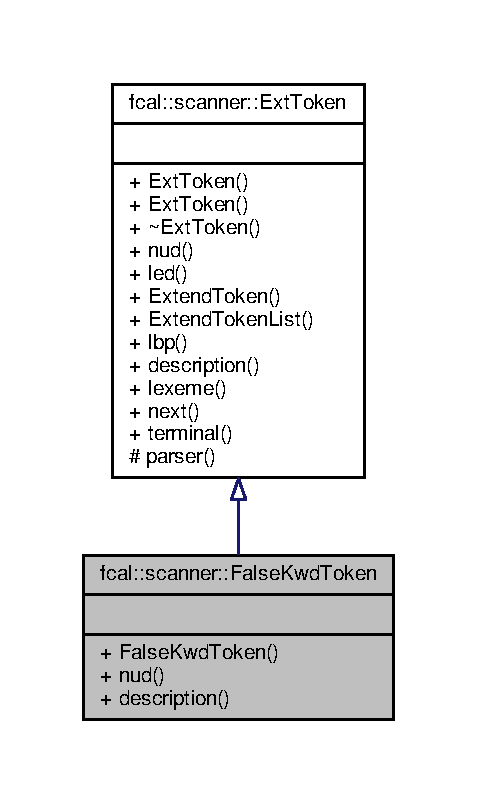
\includegraphics[width=229pt]{classfcal_1_1scanner_1_1FalseKwdToken__inherit__graph}
\end{center}
\end{figure}


Collaboration diagram for fcal\+:\+:scanner\+:\+:False\+Kwd\+Token\+:
\nopagebreak
\begin{figure}[H]
\begin{center}
\leavevmode
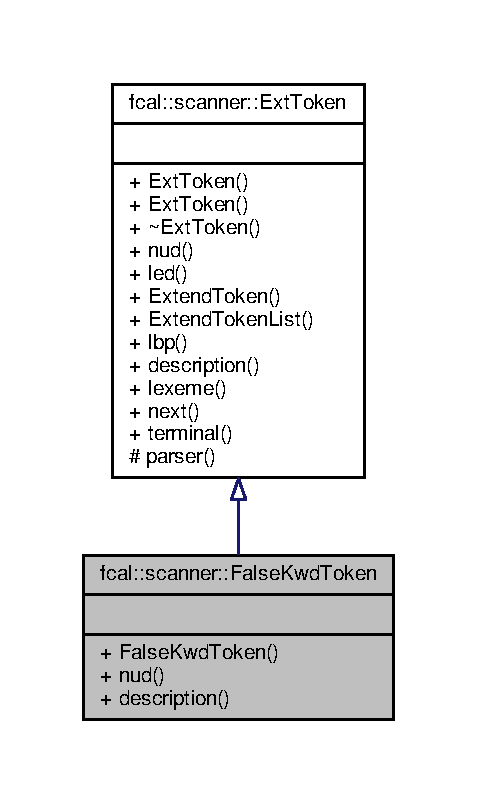
\includegraphics[width=229pt]{classfcal_1_1scanner_1_1FalseKwdToken__coll__graph}
\end{center}
\end{figure}
\subsection*{Public Member Functions}
\begin{DoxyCompactItemize}
\item 
\hyperlink{classfcal_1_1scanner_1_1FalseKwdToken_ac35ad99acd8ed526d7e7a5d5216b060e}{False\+Kwd\+Token} (\hyperlink{classfcal_1_1parser_1_1Parser}{parser\+::\+Parser} $\ast$p, \hyperlink{classfcal_1_1scanner_1_1Token}{Token} $\ast$t)
\item 
\hyperlink{classfcal_1_1parser_1_1ParseResult}{parser\+::\+Parse\+Result} \hyperlink{classfcal_1_1scanner_1_1FalseKwdToken_a57566622065242fe629d5f991022cdac}{nud} ()
\item 
std\+::string \hyperlink{classfcal_1_1scanner_1_1FalseKwdToken_ad03d22a5baf8377d409dcae104cfc997}{description} ()
\end{DoxyCompactItemize}
\subsection*{Additional Inherited Members}


\subsection{Constructor \& Destructor Documentation}
\index{fcal\+::scanner\+::\+False\+Kwd\+Token@{fcal\+::scanner\+::\+False\+Kwd\+Token}!False\+Kwd\+Token@{False\+Kwd\+Token}}
\index{False\+Kwd\+Token@{False\+Kwd\+Token}!fcal\+::scanner\+::\+False\+Kwd\+Token@{fcal\+::scanner\+::\+False\+Kwd\+Token}}
\subsubsection[{\texorpdfstring{False\+Kwd\+Token(parser\+::\+Parser $\ast$p, Token $\ast$t)}{FalseKwdToken(parser::Parser *p, Token *t)}}]{\setlength{\rightskip}{0pt plus 5cm}fcal\+::scanner\+::\+False\+Kwd\+Token\+::\+False\+Kwd\+Token (
\begin{DoxyParamCaption}
\item[{{\bf parser\+::\+Parser} $\ast$}]{p, }
\item[{{\bf Token} $\ast$}]{t}
\end{DoxyParamCaption}
)\hspace{0.3cm}{\ttfamily [inline]}}\hypertarget{classfcal_1_1scanner_1_1FalseKwdToken_ac35ad99acd8ed526d7e7a5d5216b060e}{}\label{classfcal_1_1scanner_1_1FalseKwdToken_ac35ad99acd8ed526d7e7a5d5216b060e}


\subsection{Member Function Documentation}
\index{fcal\+::scanner\+::\+False\+Kwd\+Token@{fcal\+::scanner\+::\+False\+Kwd\+Token}!description@{description}}
\index{description@{description}!fcal\+::scanner\+::\+False\+Kwd\+Token@{fcal\+::scanner\+::\+False\+Kwd\+Token}}
\subsubsection[{\texorpdfstring{description()}{description()}}]{\setlength{\rightskip}{0pt plus 5cm}std\+::string fcal\+::scanner\+::\+False\+Kwd\+Token\+::description (
\begin{DoxyParamCaption}
{}
\end{DoxyParamCaption}
)\hspace{0.3cm}{\ttfamily [inline]}, {\ttfamily [virtual]}}\hypertarget{classfcal_1_1scanner_1_1FalseKwdToken_ad03d22a5baf8377d409dcae104cfc997}{}\label{classfcal_1_1scanner_1_1FalseKwdToken_ad03d22a5baf8377d409dcae104cfc997}


Reimplemented from \hyperlink{classfcal_1_1scanner_1_1ExtToken_a29a72149492d7fef7968a1b894d334c7}{fcal\+::scanner\+::\+Ext\+Token}.

\index{fcal\+::scanner\+::\+False\+Kwd\+Token@{fcal\+::scanner\+::\+False\+Kwd\+Token}!nud@{nud}}
\index{nud@{nud}!fcal\+::scanner\+::\+False\+Kwd\+Token@{fcal\+::scanner\+::\+False\+Kwd\+Token}}
\subsubsection[{\texorpdfstring{nud()}{nud()}}]{\setlength{\rightskip}{0pt plus 5cm}{\bf parser\+::\+Parse\+Result} fcal\+::scanner\+::\+False\+Kwd\+Token\+::nud (
\begin{DoxyParamCaption}
\item[{void}]{}
\end{DoxyParamCaption}
)\hspace{0.3cm}{\ttfamily [inline]}, {\ttfamily [virtual]}}\hypertarget{classfcal_1_1scanner_1_1FalseKwdToken_a57566622065242fe629d5f991022cdac}{}\label{classfcal_1_1scanner_1_1FalseKwdToken_a57566622065242fe629d5f991022cdac}


Reimplemented from \hyperlink{classfcal_1_1scanner_1_1ExtToken_a2e1ca27a07d55593ffd67780dbcad7dd}{fcal\+::scanner\+::\+Ext\+Token}.



The documentation for this class was generated from the following file\+:\begin{DoxyCompactItemize}
\item 
include/\hyperlink{ext__token_8h}{ext\+\_\+token.\+h}\end{DoxyCompactItemize}

\hypertarget{classfcal_1_1ast_1_1FloatConstExpr}{}\section{fcal\+:\+:ast\+:\+:Float\+Const\+Expr Class Reference}
\label{classfcal_1_1ast_1_1FloatConstExpr}\index{fcal\+::ast\+::\+Float\+Const\+Expr@{fcal\+::ast\+::\+Float\+Const\+Expr}}


{\ttfamily \#include $<$ast.\+h$>$}



Inheritance diagram for fcal\+:\+:ast\+:\+:Float\+Const\+Expr\+:
\nopagebreak
\begin{figure}[H]
\begin{center}
\leavevmode
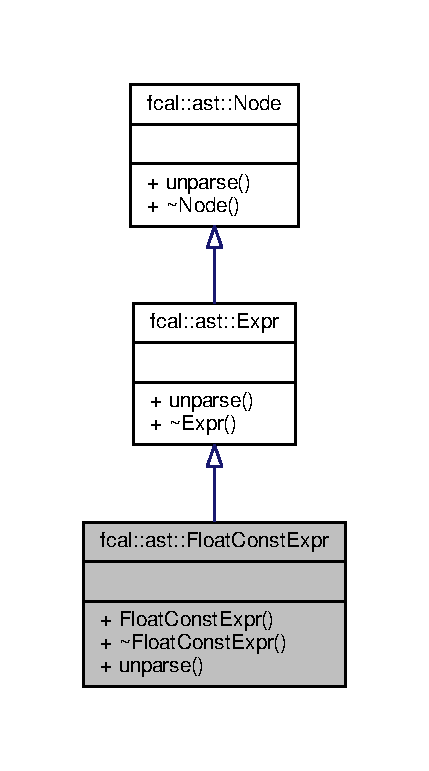
\includegraphics[width=206pt]{classfcal_1_1ast_1_1FloatConstExpr__inherit__graph}
\end{center}
\end{figure}


Collaboration diagram for fcal\+:\+:ast\+:\+:Float\+Const\+Expr\+:
\nopagebreak
\begin{figure}[H]
\begin{center}
\leavevmode
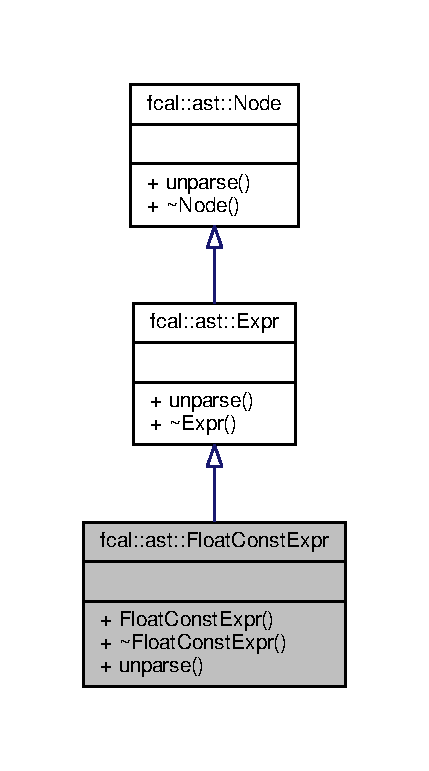
\includegraphics[width=206pt]{classfcal_1_1ast_1_1FloatConstExpr__coll__graph}
\end{center}
\end{figure}
\subsection*{Public Member Functions}
\begin{DoxyCompactItemize}
\item 
\hyperlink{classfcal_1_1ast_1_1FloatConstExpr_a162cf50d6cc7d6bf7f7b50187f9a370a}{Float\+Const\+Expr} (std\+::string f)
\item 
\hyperlink{classfcal_1_1ast_1_1FloatConstExpr_a9c4b14923e453f33bcf93e5e8f50d2be}{$\sim$\+Float\+Const\+Expr} ()
\item 
std\+::string \hyperlink{classfcal_1_1ast_1_1FloatConstExpr_ac43f676dc814852231c0ac263d1a2628}{unparse} ()
\end{DoxyCompactItemize}


\subsection{Constructor \& Destructor Documentation}
\index{fcal\+::ast\+::\+Float\+Const\+Expr@{fcal\+::ast\+::\+Float\+Const\+Expr}!Float\+Const\+Expr@{Float\+Const\+Expr}}
\index{Float\+Const\+Expr@{Float\+Const\+Expr}!fcal\+::ast\+::\+Float\+Const\+Expr@{fcal\+::ast\+::\+Float\+Const\+Expr}}
\subsubsection[{\texorpdfstring{Float\+Const\+Expr(std\+::string f)}{FloatConstExpr(std::string f)}}]{\setlength{\rightskip}{0pt plus 5cm}fcal\+::ast\+::\+Float\+Const\+Expr\+::\+Float\+Const\+Expr (
\begin{DoxyParamCaption}
\item[{std\+::string}]{f}
\end{DoxyParamCaption}
)\hspace{0.3cm}{\ttfamily [inline]}, {\ttfamily [explicit]}}\hypertarget{classfcal_1_1ast_1_1FloatConstExpr_a162cf50d6cc7d6bf7f7b50187f9a370a}{}\label{classfcal_1_1ast_1_1FloatConstExpr_a162cf50d6cc7d6bf7f7b50187f9a370a}
\index{fcal\+::ast\+::\+Float\+Const\+Expr@{fcal\+::ast\+::\+Float\+Const\+Expr}!````~Float\+Const\+Expr@{$\sim$\+Float\+Const\+Expr}}
\index{````~Float\+Const\+Expr@{$\sim$\+Float\+Const\+Expr}!fcal\+::ast\+::\+Float\+Const\+Expr@{fcal\+::ast\+::\+Float\+Const\+Expr}}
\subsubsection[{\texorpdfstring{$\sim$\+Float\+Const\+Expr()}{~FloatConstExpr()}}]{\setlength{\rightskip}{0pt plus 5cm}fcal\+::ast\+::\+Float\+Const\+Expr\+::$\sim$\+Float\+Const\+Expr (
\begin{DoxyParamCaption}
{}
\end{DoxyParamCaption}
)\hspace{0.3cm}{\ttfamily [inline]}}\hypertarget{classfcal_1_1ast_1_1FloatConstExpr_a9c4b14923e453f33bcf93e5e8f50d2be}{}\label{classfcal_1_1ast_1_1FloatConstExpr_a9c4b14923e453f33bcf93e5e8f50d2be}


\subsection{Member Function Documentation}
\index{fcal\+::ast\+::\+Float\+Const\+Expr@{fcal\+::ast\+::\+Float\+Const\+Expr}!unparse@{unparse}}
\index{unparse@{unparse}!fcal\+::ast\+::\+Float\+Const\+Expr@{fcal\+::ast\+::\+Float\+Const\+Expr}}
\subsubsection[{\texorpdfstring{unparse()}{unparse()}}]{\setlength{\rightskip}{0pt plus 5cm}std\+::string fcal\+::ast\+::\+Float\+Const\+Expr\+::unparse (
\begin{DoxyParamCaption}
{}
\end{DoxyParamCaption}
)\hspace{0.3cm}{\ttfamily [inline]}, {\ttfamily [virtual]}}\hypertarget{classfcal_1_1ast_1_1FloatConstExpr_ac43f676dc814852231c0ac263d1a2628}{}\label{classfcal_1_1ast_1_1FloatConstExpr_ac43f676dc814852231c0ac263d1a2628}


Implements \hyperlink{classfcal_1_1ast_1_1Expr_adba9309749d00e7c864456fbd505f252}{fcal\+::ast\+::\+Expr}.



The documentation for this class was generated from the following file\+:\begin{DoxyCompactItemize}
\item 
include/\hyperlink{ast_8h}{ast.\+h}\end{DoxyCompactItemize}

\hypertarget{classfcal_1_1scanner_1_1FloatConstToken}{}\section{fcal\+:\+:scanner\+:\+:Float\+Const\+Token Class Reference}
\label{classfcal_1_1scanner_1_1FloatConstToken}\index{fcal\+::scanner\+::\+Float\+Const\+Token@{fcal\+::scanner\+::\+Float\+Const\+Token}}


{\ttfamily \#include $<$ext\+\_\+token.\+h$>$}



Inheritance diagram for fcal\+:\+:scanner\+:\+:Float\+Const\+Token\+:
\nopagebreak
\begin{figure}[H]
\begin{center}
\leavevmode
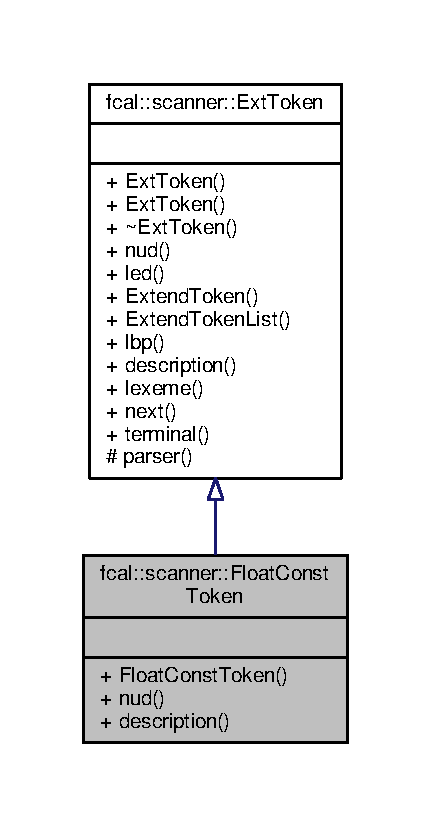
\includegraphics[width=207pt]{classfcal_1_1scanner_1_1FloatConstToken__inherit__graph}
\end{center}
\end{figure}


Collaboration diagram for fcal\+:\+:scanner\+:\+:Float\+Const\+Token\+:
\nopagebreak
\begin{figure}[H]
\begin{center}
\leavevmode
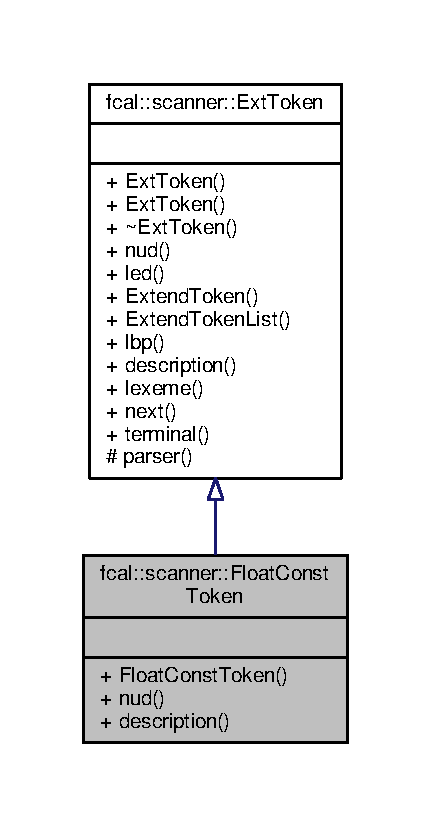
\includegraphics[width=207pt]{classfcal_1_1scanner_1_1FloatConstToken__coll__graph}
\end{center}
\end{figure}
\subsection*{Public Member Functions}
\begin{DoxyCompactItemize}
\item 
\hyperlink{classfcal_1_1scanner_1_1FloatConstToken_a715ecedd2f42b7fbcfbf564dad7909fc}{Float\+Const\+Token} (\hyperlink{classfcal_1_1parser_1_1Parser}{parser\+::\+Parser} $\ast$p, \hyperlink{classfcal_1_1scanner_1_1Token}{Token} $\ast$t)
\item 
\hyperlink{classfcal_1_1parser_1_1ParseResult}{parser\+::\+Parse\+Result} \hyperlink{classfcal_1_1scanner_1_1FloatConstToken_a7ceca1dc6b064daf39e7250d8d93a9ce}{nud} ()
\item 
std\+::string \hyperlink{classfcal_1_1scanner_1_1FloatConstToken_ac98711e11205722a389fc19682183286}{description} ()
\end{DoxyCompactItemize}
\subsection*{Additional Inherited Members}


\subsection{Constructor \& Destructor Documentation}
\index{fcal\+::scanner\+::\+Float\+Const\+Token@{fcal\+::scanner\+::\+Float\+Const\+Token}!Float\+Const\+Token@{Float\+Const\+Token}}
\index{Float\+Const\+Token@{Float\+Const\+Token}!fcal\+::scanner\+::\+Float\+Const\+Token@{fcal\+::scanner\+::\+Float\+Const\+Token}}
\subsubsection[{\texorpdfstring{Float\+Const\+Token(parser\+::\+Parser $\ast$p, Token $\ast$t)}{FloatConstToken(parser::Parser *p, Token *t)}}]{\setlength{\rightskip}{0pt plus 5cm}fcal\+::scanner\+::\+Float\+Const\+Token\+::\+Float\+Const\+Token (
\begin{DoxyParamCaption}
\item[{{\bf parser\+::\+Parser} $\ast$}]{p, }
\item[{{\bf Token} $\ast$}]{t}
\end{DoxyParamCaption}
)\hspace{0.3cm}{\ttfamily [inline]}}\hypertarget{classfcal_1_1scanner_1_1FloatConstToken_a715ecedd2f42b7fbcfbf564dad7909fc}{}\label{classfcal_1_1scanner_1_1FloatConstToken_a715ecedd2f42b7fbcfbf564dad7909fc}


\subsection{Member Function Documentation}
\index{fcal\+::scanner\+::\+Float\+Const\+Token@{fcal\+::scanner\+::\+Float\+Const\+Token}!description@{description}}
\index{description@{description}!fcal\+::scanner\+::\+Float\+Const\+Token@{fcal\+::scanner\+::\+Float\+Const\+Token}}
\subsubsection[{\texorpdfstring{description()}{description()}}]{\setlength{\rightskip}{0pt plus 5cm}std\+::string fcal\+::scanner\+::\+Float\+Const\+Token\+::description (
\begin{DoxyParamCaption}
{}
\end{DoxyParamCaption}
)\hspace{0.3cm}{\ttfamily [inline]}, {\ttfamily [virtual]}}\hypertarget{classfcal_1_1scanner_1_1FloatConstToken_ac98711e11205722a389fc19682183286}{}\label{classfcal_1_1scanner_1_1FloatConstToken_ac98711e11205722a389fc19682183286}


Reimplemented from \hyperlink{classfcal_1_1scanner_1_1ExtToken_a29a72149492d7fef7968a1b894d334c7}{fcal\+::scanner\+::\+Ext\+Token}.

\index{fcal\+::scanner\+::\+Float\+Const\+Token@{fcal\+::scanner\+::\+Float\+Const\+Token}!nud@{nud}}
\index{nud@{nud}!fcal\+::scanner\+::\+Float\+Const\+Token@{fcal\+::scanner\+::\+Float\+Const\+Token}}
\subsubsection[{\texorpdfstring{nud()}{nud()}}]{\setlength{\rightskip}{0pt plus 5cm}{\bf parser\+::\+Parse\+Result} fcal\+::scanner\+::\+Float\+Const\+Token\+::nud (
\begin{DoxyParamCaption}
\item[{void}]{}
\end{DoxyParamCaption}
)\hspace{0.3cm}{\ttfamily [inline]}, {\ttfamily [virtual]}}\hypertarget{classfcal_1_1scanner_1_1FloatConstToken_a7ceca1dc6b064daf39e7250d8d93a9ce}{}\label{classfcal_1_1scanner_1_1FloatConstToken_a7ceca1dc6b064daf39e7250d8d93a9ce}


Reimplemented from \hyperlink{classfcal_1_1scanner_1_1ExtToken_a2e1ca27a07d55593ffd67780dbcad7dd}{fcal\+::scanner\+::\+Ext\+Token}.



The documentation for this class was generated from the following file\+:\begin{DoxyCompactItemize}
\item 
include/\hyperlink{ext__token_8h}{ext\+\_\+token.\+h}\end{DoxyCompactItemize}

\hypertarget{classfcal_1_1ast_1_1FloatDecl}{}\section{fcal\+:\+:ast\+:\+:Float\+Decl Class Reference}
\label{classfcal_1_1ast_1_1FloatDecl}\index{fcal\+::ast\+::\+Float\+Decl@{fcal\+::ast\+::\+Float\+Decl}}


{\ttfamily \#include $<$ast.\+h$>$}



Inheritance diagram for fcal\+:\+:ast\+:\+:Float\+Decl\+:
\nopagebreak
\begin{figure}[H]
\begin{center}
\leavevmode
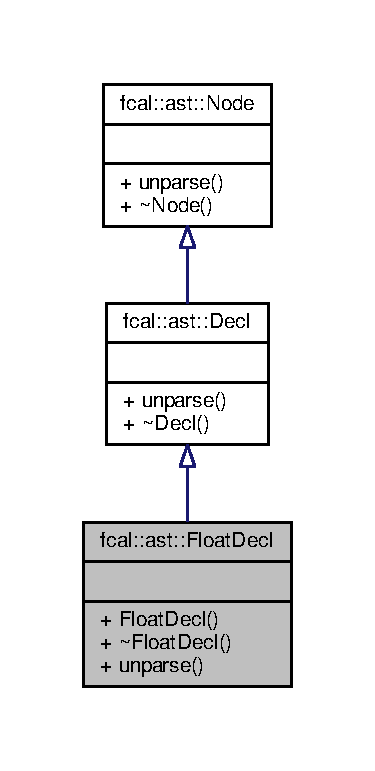
\includegraphics[width=180pt]{classfcal_1_1ast_1_1FloatDecl__inherit__graph}
\end{center}
\end{figure}


Collaboration diagram for fcal\+:\+:ast\+:\+:Float\+Decl\+:
\nopagebreak
\begin{figure}[H]
\begin{center}
\leavevmode
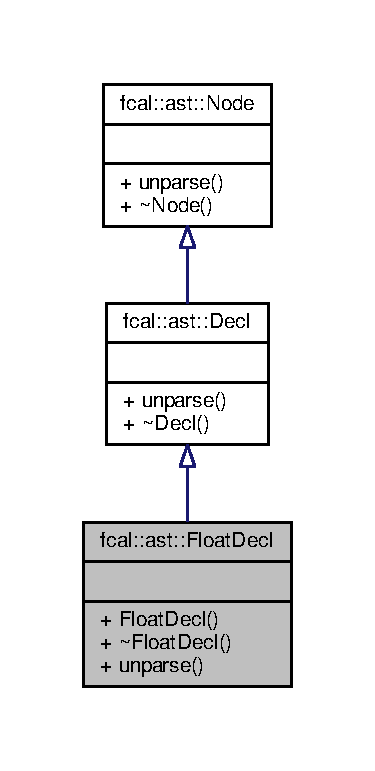
\includegraphics[width=180pt]{classfcal_1_1ast_1_1FloatDecl__coll__graph}
\end{center}
\end{figure}
\subsection*{Public Member Functions}
\begin{DoxyCompactItemize}
\item 
\hyperlink{classfcal_1_1ast_1_1FloatDecl_a125ca270dfa2c429ec03e08fff943fcc}{Float\+Decl} (std\+::string s)
\item 
\hyperlink{classfcal_1_1ast_1_1FloatDecl_a108cfa0009c375c3a204a9b96bc9f413}{$\sim$\+Float\+Decl} ()
\item 
std\+::string \hyperlink{classfcal_1_1ast_1_1FloatDecl_af2eeeb25426c98315fdb7926e16211a9}{unparse} ()
\end{DoxyCompactItemize}


\subsection{Constructor \& Destructor Documentation}
\index{fcal\+::ast\+::\+Float\+Decl@{fcal\+::ast\+::\+Float\+Decl}!Float\+Decl@{Float\+Decl}}
\index{Float\+Decl@{Float\+Decl}!fcal\+::ast\+::\+Float\+Decl@{fcal\+::ast\+::\+Float\+Decl}}
\subsubsection[{\texorpdfstring{Float\+Decl(std\+::string s)}{FloatDecl(std::string s)}}]{\setlength{\rightskip}{0pt plus 5cm}fcal\+::ast\+::\+Float\+Decl\+::\+Float\+Decl (
\begin{DoxyParamCaption}
\item[{std\+::string}]{s}
\end{DoxyParamCaption}
)\hspace{0.3cm}{\ttfamily [inline]}, {\ttfamily [explicit]}}\hypertarget{classfcal_1_1ast_1_1FloatDecl_a125ca270dfa2c429ec03e08fff943fcc}{}\label{classfcal_1_1ast_1_1FloatDecl_a125ca270dfa2c429ec03e08fff943fcc}
\index{fcal\+::ast\+::\+Float\+Decl@{fcal\+::ast\+::\+Float\+Decl}!````~Float\+Decl@{$\sim$\+Float\+Decl}}
\index{````~Float\+Decl@{$\sim$\+Float\+Decl}!fcal\+::ast\+::\+Float\+Decl@{fcal\+::ast\+::\+Float\+Decl}}
\subsubsection[{\texorpdfstring{$\sim$\+Float\+Decl()}{~FloatDecl()}}]{\setlength{\rightskip}{0pt plus 5cm}fcal\+::ast\+::\+Float\+Decl\+::$\sim$\+Float\+Decl (
\begin{DoxyParamCaption}
{}
\end{DoxyParamCaption}
)\hspace{0.3cm}{\ttfamily [inline]}}\hypertarget{classfcal_1_1ast_1_1FloatDecl_a108cfa0009c375c3a204a9b96bc9f413}{}\label{classfcal_1_1ast_1_1FloatDecl_a108cfa0009c375c3a204a9b96bc9f413}


\subsection{Member Function Documentation}
\index{fcal\+::ast\+::\+Float\+Decl@{fcal\+::ast\+::\+Float\+Decl}!unparse@{unparse}}
\index{unparse@{unparse}!fcal\+::ast\+::\+Float\+Decl@{fcal\+::ast\+::\+Float\+Decl}}
\subsubsection[{\texorpdfstring{unparse()}{unparse()}}]{\setlength{\rightskip}{0pt plus 5cm}std\+::string fcal\+::ast\+::\+Float\+Decl\+::unparse (
\begin{DoxyParamCaption}
{}
\end{DoxyParamCaption}
)\hspace{0.3cm}{\ttfamily [inline]}, {\ttfamily [virtual]}}\hypertarget{classfcal_1_1ast_1_1FloatDecl_af2eeeb25426c98315fdb7926e16211a9}{}\label{classfcal_1_1ast_1_1FloatDecl_af2eeeb25426c98315fdb7926e16211a9}


Implements \hyperlink{classfcal_1_1ast_1_1Decl_a54761cf8b990cb2d478c606be6bc29c5}{fcal\+::ast\+::\+Decl}.



The documentation for this class was generated from the following file\+:\begin{DoxyCompactItemize}
\item 
include/\hyperlink{ast_8h}{ast.\+h}\end{DoxyCompactItemize}

\hypertarget{classfcal_1_1scanner_1_1ForwardSlashToken}{}\section{fcal\+:\+:scanner\+:\+:Forward\+Slash\+Token Class Reference}
\label{classfcal_1_1scanner_1_1ForwardSlashToken}\index{fcal\+::scanner\+::\+Forward\+Slash\+Token@{fcal\+::scanner\+::\+Forward\+Slash\+Token}}


{\ttfamily \#include $<$ext\+\_\+token.\+h$>$}



Inheritance diagram for fcal\+:\+:scanner\+:\+:Forward\+Slash\+Token\+:
\nopagebreak
\begin{figure}[H]
\begin{center}
\leavevmode
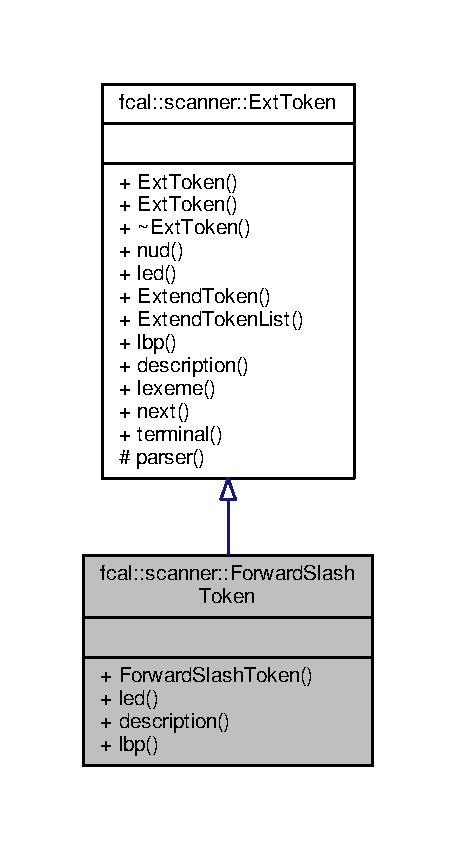
\includegraphics[width=219pt]{classfcal_1_1scanner_1_1ForwardSlashToken__inherit__graph}
\end{center}
\end{figure}


Collaboration diagram for fcal\+:\+:scanner\+:\+:Forward\+Slash\+Token\+:
\nopagebreak
\begin{figure}[H]
\begin{center}
\leavevmode
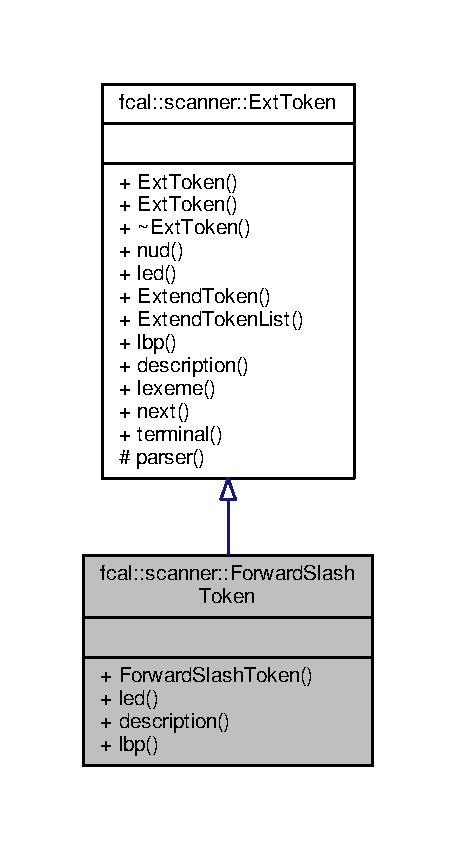
\includegraphics[width=219pt]{classfcal_1_1scanner_1_1ForwardSlashToken__coll__graph}
\end{center}
\end{figure}
\subsection*{Public Member Functions}
\begin{DoxyCompactItemize}
\item 
\hyperlink{classfcal_1_1scanner_1_1ForwardSlashToken_a78339cc748c46b86c73945ea345e6e1d}{Forward\+Slash\+Token} (\hyperlink{classfcal_1_1parser_1_1Parser}{parser\+::\+Parser} $\ast$p, \hyperlink{classfcal_1_1scanner_1_1Token}{Token} $\ast$t)
\item 
\hyperlink{classfcal_1_1parser_1_1ParseResult}{parser\+::\+Parse\+Result} \hyperlink{classfcal_1_1scanner_1_1ForwardSlashToken_a75ba06718e3faa1d53c62182d0f7b1db}{led} (\hyperlink{classfcal_1_1parser_1_1ParseResult}{parser\+::\+Parse\+Result} left)
\item 
std\+::string \hyperlink{classfcal_1_1scanner_1_1ForwardSlashToken_a04d39d9ea4cbb704862d33cb447de83b}{description} ()
\item 
int \hyperlink{classfcal_1_1scanner_1_1ForwardSlashToken_ae2c4a56a7c81f1f9d697ccca1e95c153}{lbp} ()
\end{DoxyCompactItemize}
\subsection*{Additional Inherited Members}


\subsection{Constructor \& Destructor Documentation}
\index{fcal\+::scanner\+::\+Forward\+Slash\+Token@{fcal\+::scanner\+::\+Forward\+Slash\+Token}!Forward\+Slash\+Token@{Forward\+Slash\+Token}}
\index{Forward\+Slash\+Token@{Forward\+Slash\+Token}!fcal\+::scanner\+::\+Forward\+Slash\+Token@{fcal\+::scanner\+::\+Forward\+Slash\+Token}}
\subsubsection[{\texorpdfstring{Forward\+Slash\+Token(parser\+::\+Parser $\ast$p, Token $\ast$t)}{ForwardSlashToken(parser::Parser *p, Token *t)}}]{\setlength{\rightskip}{0pt plus 5cm}fcal\+::scanner\+::\+Forward\+Slash\+Token\+::\+Forward\+Slash\+Token (
\begin{DoxyParamCaption}
\item[{{\bf parser\+::\+Parser} $\ast$}]{p, }
\item[{{\bf Token} $\ast$}]{t}
\end{DoxyParamCaption}
)\hspace{0.3cm}{\ttfamily [inline]}}\hypertarget{classfcal_1_1scanner_1_1ForwardSlashToken_a78339cc748c46b86c73945ea345e6e1d}{}\label{classfcal_1_1scanner_1_1ForwardSlashToken_a78339cc748c46b86c73945ea345e6e1d}


\subsection{Member Function Documentation}
\index{fcal\+::scanner\+::\+Forward\+Slash\+Token@{fcal\+::scanner\+::\+Forward\+Slash\+Token}!description@{description}}
\index{description@{description}!fcal\+::scanner\+::\+Forward\+Slash\+Token@{fcal\+::scanner\+::\+Forward\+Slash\+Token}}
\subsubsection[{\texorpdfstring{description()}{description()}}]{\setlength{\rightskip}{0pt plus 5cm}std\+::string fcal\+::scanner\+::\+Forward\+Slash\+Token\+::description (
\begin{DoxyParamCaption}
{}
\end{DoxyParamCaption}
)\hspace{0.3cm}{\ttfamily [inline]}, {\ttfamily [virtual]}}\hypertarget{classfcal_1_1scanner_1_1ForwardSlashToken_a04d39d9ea4cbb704862d33cb447de83b}{}\label{classfcal_1_1scanner_1_1ForwardSlashToken_a04d39d9ea4cbb704862d33cb447de83b}


Reimplemented from \hyperlink{classfcal_1_1scanner_1_1ExtToken_a29a72149492d7fef7968a1b894d334c7}{fcal\+::scanner\+::\+Ext\+Token}.

\index{fcal\+::scanner\+::\+Forward\+Slash\+Token@{fcal\+::scanner\+::\+Forward\+Slash\+Token}!lbp@{lbp}}
\index{lbp@{lbp}!fcal\+::scanner\+::\+Forward\+Slash\+Token@{fcal\+::scanner\+::\+Forward\+Slash\+Token}}
\subsubsection[{\texorpdfstring{lbp()}{lbp()}}]{\setlength{\rightskip}{0pt plus 5cm}int fcal\+::scanner\+::\+Forward\+Slash\+Token\+::lbp (
\begin{DoxyParamCaption}
{}
\end{DoxyParamCaption}
)\hspace{0.3cm}{\ttfamily [inline]}, {\ttfamily [virtual]}}\hypertarget{classfcal_1_1scanner_1_1ForwardSlashToken_ae2c4a56a7c81f1f9d697ccca1e95c153}{}\label{classfcal_1_1scanner_1_1ForwardSlashToken_ae2c4a56a7c81f1f9d697ccca1e95c153}


Reimplemented from \hyperlink{classfcal_1_1scanner_1_1ExtToken_adecef3770f08e5a26f103ab62171cc91}{fcal\+::scanner\+::\+Ext\+Token}.

\index{fcal\+::scanner\+::\+Forward\+Slash\+Token@{fcal\+::scanner\+::\+Forward\+Slash\+Token}!led@{led}}
\index{led@{led}!fcal\+::scanner\+::\+Forward\+Slash\+Token@{fcal\+::scanner\+::\+Forward\+Slash\+Token}}
\subsubsection[{\texorpdfstring{led(parser\+::\+Parse\+Result left)}{led(parser::ParseResult left)}}]{\setlength{\rightskip}{0pt plus 5cm}{\bf parser\+::\+Parse\+Result} fcal\+::scanner\+::\+Forward\+Slash\+Token\+::led (
\begin{DoxyParamCaption}
\item[{{\bf parser\+::\+Parse\+Result}}]{left}
\end{DoxyParamCaption}
)\hspace{0.3cm}{\ttfamily [inline]}, {\ttfamily [virtual]}}\hypertarget{classfcal_1_1scanner_1_1ForwardSlashToken_a75ba06718e3faa1d53c62182d0f7b1db}{}\label{classfcal_1_1scanner_1_1ForwardSlashToken_a75ba06718e3faa1d53c62182d0f7b1db}


Reimplemented from \hyperlink{classfcal_1_1scanner_1_1ExtToken_a42c352ef5e019a1155be80b4a40deb38}{fcal\+::scanner\+::\+Ext\+Token}.



The documentation for this class was generated from the following file\+:\begin{DoxyCompactItemize}
\item 
include/\hyperlink{ext__token_8h}{ext\+\_\+token.\+h}\end{DoxyCompactItemize}

\hypertarget{classfcal_1_1ast_1_1GreaterEqualExpr}{}\section{fcal\+:\+:ast\+:\+:Greater\+Equal\+Expr Class Reference}
\label{classfcal_1_1ast_1_1GreaterEqualExpr}\index{fcal\+::ast\+::\+Greater\+Equal\+Expr@{fcal\+::ast\+::\+Greater\+Equal\+Expr}}


{\ttfamily \#include $<$ast.\+h$>$}



Inheritance diagram for fcal\+:\+:ast\+:\+:Greater\+Equal\+Expr\+:
\nopagebreak
\begin{figure}[H]
\begin{center}
\leavevmode
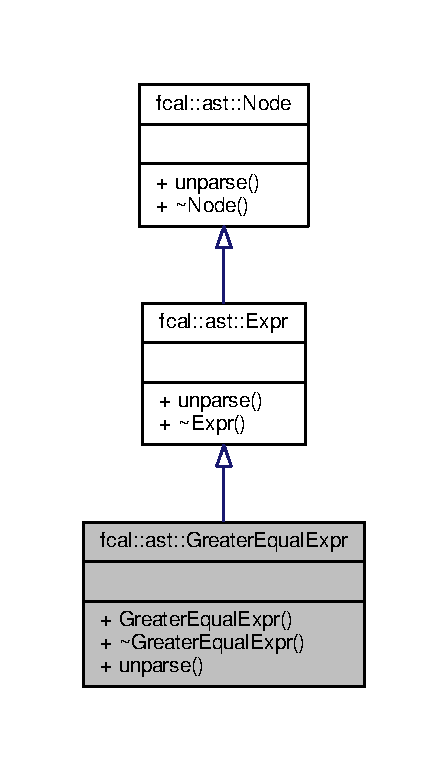
\includegraphics[width=215pt]{classfcal_1_1ast_1_1GreaterEqualExpr__inherit__graph}
\end{center}
\end{figure}


Collaboration diagram for fcal\+:\+:ast\+:\+:Greater\+Equal\+Expr\+:
\nopagebreak
\begin{figure}[H]
\begin{center}
\leavevmode
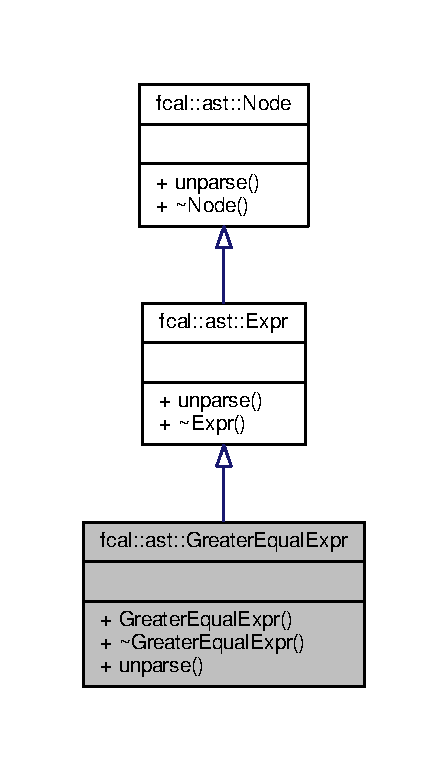
\includegraphics[width=215pt]{classfcal_1_1ast_1_1GreaterEqualExpr__coll__graph}
\end{center}
\end{figure}
\subsection*{Public Member Functions}
\begin{DoxyCompactItemize}
\item 
\hyperlink{classfcal_1_1ast_1_1GreaterEqualExpr_a9dba923841463a370103372a14d337ff}{Greater\+Equal\+Expr} (\hyperlink{classfcal_1_1ast_1_1Expr}{Expr} $\ast$e1, \hyperlink{classfcal_1_1ast_1_1Expr}{Expr} $\ast$e2)
\item 
\hyperlink{classfcal_1_1ast_1_1GreaterEqualExpr_a3e5a0544dd116b53a0376324e7bf6ac0}{$\sim$\+Greater\+Equal\+Expr} ()
\item 
std\+::string \hyperlink{classfcal_1_1ast_1_1GreaterEqualExpr_a1ae9a0851f31b4740ffb8a35a9014478}{unparse} ()
\end{DoxyCompactItemize}


\subsection{Constructor \& Destructor Documentation}
\index{fcal\+::ast\+::\+Greater\+Equal\+Expr@{fcal\+::ast\+::\+Greater\+Equal\+Expr}!Greater\+Equal\+Expr@{Greater\+Equal\+Expr}}
\index{Greater\+Equal\+Expr@{Greater\+Equal\+Expr}!fcal\+::ast\+::\+Greater\+Equal\+Expr@{fcal\+::ast\+::\+Greater\+Equal\+Expr}}
\subsubsection[{\texorpdfstring{Greater\+Equal\+Expr(\+Expr $\ast$e1, Expr $\ast$e2)}{GreaterEqualExpr(Expr *e1, Expr *e2)}}]{\setlength{\rightskip}{0pt plus 5cm}fcal\+::ast\+::\+Greater\+Equal\+Expr\+::\+Greater\+Equal\+Expr (
\begin{DoxyParamCaption}
\item[{{\bf Expr} $\ast$}]{e1, }
\item[{{\bf Expr} $\ast$}]{e2}
\end{DoxyParamCaption}
)\hspace{0.3cm}{\ttfamily [inline]}}\hypertarget{classfcal_1_1ast_1_1GreaterEqualExpr_a9dba923841463a370103372a14d337ff}{}\label{classfcal_1_1ast_1_1GreaterEqualExpr_a9dba923841463a370103372a14d337ff}
\index{fcal\+::ast\+::\+Greater\+Equal\+Expr@{fcal\+::ast\+::\+Greater\+Equal\+Expr}!````~Greater\+Equal\+Expr@{$\sim$\+Greater\+Equal\+Expr}}
\index{````~Greater\+Equal\+Expr@{$\sim$\+Greater\+Equal\+Expr}!fcal\+::ast\+::\+Greater\+Equal\+Expr@{fcal\+::ast\+::\+Greater\+Equal\+Expr}}
\subsubsection[{\texorpdfstring{$\sim$\+Greater\+Equal\+Expr()}{~GreaterEqualExpr()}}]{\setlength{\rightskip}{0pt plus 5cm}fcal\+::ast\+::\+Greater\+Equal\+Expr\+::$\sim$\+Greater\+Equal\+Expr (
\begin{DoxyParamCaption}
{}
\end{DoxyParamCaption}
)\hspace{0.3cm}{\ttfamily [inline]}}\hypertarget{classfcal_1_1ast_1_1GreaterEqualExpr_a3e5a0544dd116b53a0376324e7bf6ac0}{}\label{classfcal_1_1ast_1_1GreaterEqualExpr_a3e5a0544dd116b53a0376324e7bf6ac0}


\subsection{Member Function Documentation}
\index{fcal\+::ast\+::\+Greater\+Equal\+Expr@{fcal\+::ast\+::\+Greater\+Equal\+Expr}!unparse@{unparse}}
\index{unparse@{unparse}!fcal\+::ast\+::\+Greater\+Equal\+Expr@{fcal\+::ast\+::\+Greater\+Equal\+Expr}}
\subsubsection[{\texorpdfstring{unparse()}{unparse()}}]{\setlength{\rightskip}{0pt plus 5cm}std\+::string fcal\+::ast\+::\+Greater\+Equal\+Expr\+::unparse (
\begin{DoxyParamCaption}
{}
\end{DoxyParamCaption}
)\hspace{0.3cm}{\ttfamily [inline]}, {\ttfamily [virtual]}}\hypertarget{classfcal_1_1ast_1_1GreaterEqualExpr_a1ae9a0851f31b4740ffb8a35a9014478}{}\label{classfcal_1_1ast_1_1GreaterEqualExpr_a1ae9a0851f31b4740ffb8a35a9014478}


Implements \hyperlink{classfcal_1_1ast_1_1Expr_adba9309749d00e7c864456fbd505f252}{fcal\+::ast\+::\+Expr}.



The documentation for this class was generated from the following file\+:\begin{DoxyCompactItemize}
\item 
include/\hyperlink{ast_8h}{ast.\+h}\end{DoxyCompactItemize}

\hypertarget{classfcal_1_1ast_1_1GreaterExpr}{}\section{fcal\+:\+:ast\+:\+:Greater\+Expr Class Reference}
\label{classfcal_1_1ast_1_1GreaterExpr}\index{fcal\+::ast\+::\+Greater\+Expr@{fcal\+::ast\+::\+Greater\+Expr}}


{\ttfamily \#include $<$ast.\+h$>$}



Inheritance diagram for fcal\+:\+:ast\+:\+:Greater\+Expr\+:
\nopagebreak
\begin{figure}[H]
\begin{center}
\leavevmode
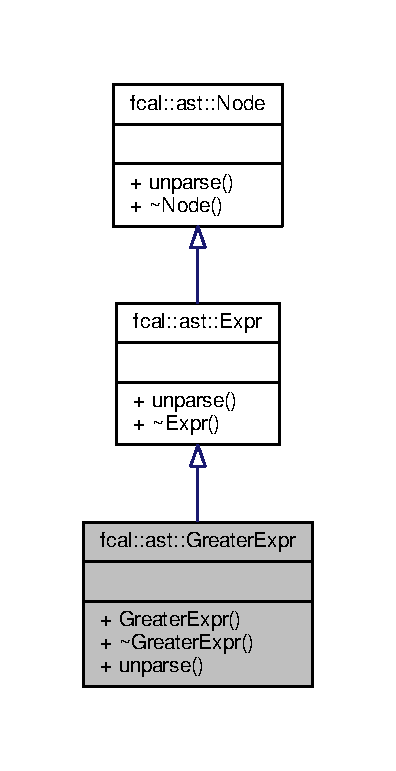
\includegraphics[width=190pt]{classfcal_1_1ast_1_1GreaterExpr__inherit__graph}
\end{center}
\end{figure}


Collaboration diagram for fcal\+:\+:ast\+:\+:Greater\+Expr\+:
\nopagebreak
\begin{figure}[H]
\begin{center}
\leavevmode
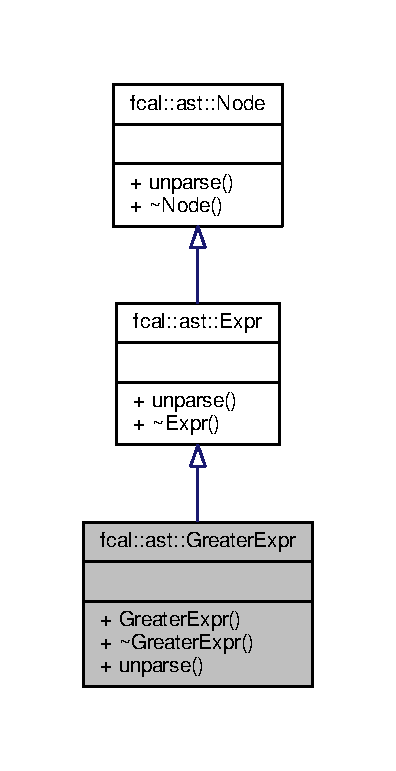
\includegraphics[width=190pt]{classfcal_1_1ast_1_1GreaterExpr__coll__graph}
\end{center}
\end{figure}
\subsection*{Public Member Functions}
\begin{DoxyCompactItemize}
\item 
\hyperlink{classfcal_1_1ast_1_1GreaterExpr_add7bba63f86e25bcbd9c12da1dc712d4}{Greater\+Expr} (\hyperlink{classfcal_1_1ast_1_1Expr}{Expr} $\ast$e1, \hyperlink{classfcal_1_1ast_1_1Expr}{Expr} $\ast$e2)
\item 
\hyperlink{classfcal_1_1ast_1_1GreaterExpr_a42d97746b3f5dabd587a34a411815cbe}{$\sim$\+Greater\+Expr} ()
\item 
std\+::string \hyperlink{classfcal_1_1ast_1_1GreaterExpr_ad5bd1acf689d89841845e14d63e42e16}{unparse} ()
\end{DoxyCompactItemize}


\subsection{Constructor \& Destructor Documentation}
\index{fcal\+::ast\+::\+Greater\+Expr@{fcal\+::ast\+::\+Greater\+Expr}!Greater\+Expr@{Greater\+Expr}}
\index{Greater\+Expr@{Greater\+Expr}!fcal\+::ast\+::\+Greater\+Expr@{fcal\+::ast\+::\+Greater\+Expr}}
\subsubsection[{\texorpdfstring{Greater\+Expr(\+Expr $\ast$e1, Expr $\ast$e2)}{GreaterExpr(Expr *e1, Expr *e2)}}]{\setlength{\rightskip}{0pt plus 5cm}fcal\+::ast\+::\+Greater\+Expr\+::\+Greater\+Expr (
\begin{DoxyParamCaption}
\item[{{\bf Expr} $\ast$}]{e1, }
\item[{{\bf Expr} $\ast$}]{e2}
\end{DoxyParamCaption}
)\hspace{0.3cm}{\ttfamily [inline]}}\hypertarget{classfcal_1_1ast_1_1GreaterExpr_add7bba63f86e25bcbd9c12da1dc712d4}{}\label{classfcal_1_1ast_1_1GreaterExpr_add7bba63f86e25bcbd9c12da1dc712d4}
\index{fcal\+::ast\+::\+Greater\+Expr@{fcal\+::ast\+::\+Greater\+Expr}!````~Greater\+Expr@{$\sim$\+Greater\+Expr}}
\index{````~Greater\+Expr@{$\sim$\+Greater\+Expr}!fcal\+::ast\+::\+Greater\+Expr@{fcal\+::ast\+::\+Greater\+Expr}}
\subsubsection[{\texorpdfstring{$\sim$\+Greater\+Expr()}{~GreaterExpr()}}]{\setlength{\rightskip}{0pt plus 5cm}fcal\+::ast\+::\+Greater\+Expr\+::$\sim$\+Greater\+Expr (
\begin{DoxyParamCaption}
{}
\end{DoxyParamCaption}
)\hspace{0.3cm}{\ttfamily [inline]}}\hypertarget{classfcal_1_1ast_1_1GreaterExpr_a42d97746b3f5dabd587a34a411815cbe}{}\label{classfcal_1_1ast_1_1GreaterExpr_a42d97746b3f5dabd587a34a411815cbe}


\subsection{Member Function Documentation}
\index{fcal\+::ast\+::\+Greater\+Expr@{fcal\+::ast\+::\+Greater\+Expr}!unparse@{unparse}}
\index{unparse@{unparse}!fcal\+::ast\+::\+Greater\+Expr@{fcal\+::ast\+::\+Greater\+Expr}}
\subsubsection[{\texorpdfstring{unparse()}{unparse()}}]{\setlength{\rightskip}{0pt plus 5cm}std\+::string fcal\+::ast\+::\+Greater\+Expr\+::unparse (
\begin{DoxyParamCaption}
{}
\end{DoxyParamCaption}
)\hspace{0.3cm}{\ttfamily [inline]}, {\ttfamily [virtual]}}\hypertarget{classfcal_1_1ast_1_1GreaterExpr_ad5bd1acf689d89841845e14d63e42e16}{}\label{classfcal_1_1ast_1_1GreaterExpr_ad5bd1acf689d89841845e14d63e42e16}


Implements \hyperlink{classfcal_1_1ast_1_1Expr_adba9309749d00e7c864456fbd505f252}{fcal\+::ast\+::\+Expr}.



The documentation for this class was generated from the following file\+:\begin{DoxyCompactItemize}
\item 
include/\hyperlink{ast_8h}{ast.\+h}\end{DoxyCompactItemize}

\hypertarget{classfcal_1_1ast_1_1IfElseStmt}{}\section{fcal\+:\+:ast\+:\+:If\+Else\+Stmt Class Reference}
\label{classfcal_1_1ast_1_1IfElseStmt}\index{fcal\+::ast\+::\+If\+Else\+Stmt@{fcal\+::ast\+::\+If\+Else\+Stmt}}


{\ttfamily \#include $<$ast.\+h$>$}



Inheritance diagram for fcal\+:\+:ast\+:\+:If\+Else\+Stmt\+:
\nopagebreak
\begin{figure}[H]
\begin{center}
\leavevmode
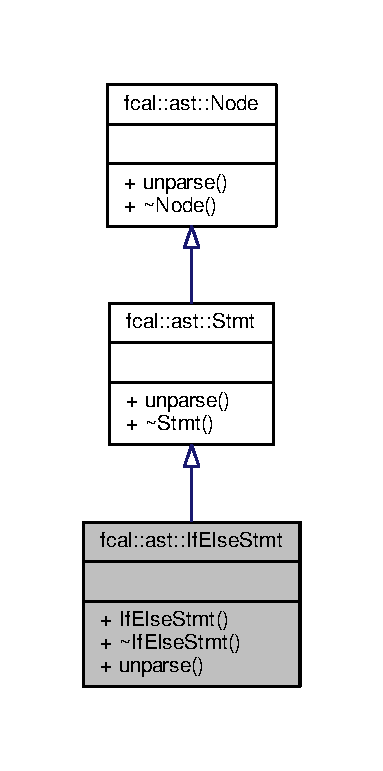
\includegraphics[width=184pt]{classfcal_1_1ast_1_1IfElseStmt__inherit__graph}
\end{center}
\end{figure}


Collaboration diagram for fcal\+:\+:ast\+:\+:If\+Else\+Stmt\+:
\nopagebreak
\begin{figure}[H]
\begin{center}
\leavevmode
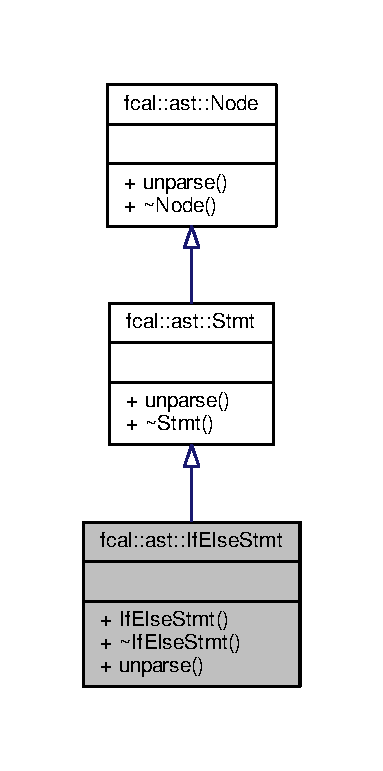
\includegraphics[width=184pt]{classfcal_1_1ast_1_1IfElseStmt__coll__graph}
\end{center}
\end{figure}
\subsection*{Public Member Functions}
\begin{DoxyCompactItemize}
\item 
\hyperlink{classfcal_1_1ast_1_1IfElseStmt_abaf8db62e3ca16be8bfd7a563a0f0cfe}{If\+Else\+Stmt} (\hyperlink{classfcal_1_1ast_1_1Expr}{Expr} $\ast$e, \hyperlink{classfcal_1_1ast_1_1Stmt}{Stmt} $\ast$s1, \hyperlink{classfcal_1_1ast_1_1Stmt}{Stmt} $\ast$s2)
\item 
\hyperlink{classfcal_1_1ast_1_1IfElseStmt_acf5d8788769fb49588be5f4d5acef5d9}{$\sim$\+If\+Else\+Stmt} ()
\item 
std\+::string \hyperlink{classfcal_1_1ast_1_1IfElseStmt_a58584903e7e9480773ca5be804342721}{unparse} ()
\end{DoxyCompactItemize}


\subsection{Constructor \& Destructor Documentation}
\index{fcal\+::ast\+::\+If\+Else\+Stmt@{fcal\+::ast\+::\+If\+Else\+Stmt}!If\+Else\+Stmt@{If\+Else\+Stmt}}
\index{If\+Else\+Stmt@{If\+Else\+Stmt}!fcal\+::ast\+::\+If\+Else\+Stmt@{fcal\+::ast\+::\+If\+Else\+Stmt}}
\subsubsection[{\texorpdfstring{If\+Else\+Stmt(\+Expr $\ast$e, Stmt $\ast$s1, Stmt $\ast$s2)}{IfElseStmt(Expr *e, Stmt *s1, Stmt *s2)}}]{\setlength{\rightskip}{0pt plus 5cm}fcal\+::ast\+::\+If\+Else\+Stmt\+::\+If\+Else\+Stmt (
\begin{DoxyParamCaption}
\item[{{\bf Expr} $\ast$}]{e, }
\item[{{\bf Stmt} $\ast$}]{s1, }
\item[{{\bf Stmt} $\ast$}]{s2}
\end{DoxyParamCaption}
)\hspace{0.3cm}{\ttfamily [inline]}}\hypertarget{classfcal_1_1ast_1_1IfElseStmt_abaf8db62e3ca16be8bfd7a563a0f0cfe}{}\label{classfcal_1_1ast_1_1IfElseStmt_abaf8db62e3ca16be8bfd7a563a0f0cfe}
\index{fcal\+::ast\+::\+If\+Else\+Stmt@{fcal\+::ast\+::\+If\+Else\+Stmt}!````~If\+Else\+Stmt@{$\sim$\+If\+Else\+Stmt}}
\index{````~If\+Else\+Stmt@{$\sim$\+If\+Else\+Stmt}!fcal\+::ast\+::\+If\+Else\+Stmt@{fcal\+::ast\+::\+If\+Else\+Stmt}}
\subsubsection[{\texorpdfstring{$\sim$\+If\+Else\+Stmt()}{~IfElseStmt()}}]{\setlength{\rightskip}{0pt plus 5cm}fcal\+::ast\+::\+If\+Else\+Stmt\+::$\sim$\+If\+Else\+Stmt (
\begin{DoxyParamCaption}
{}
\end{DoxyParamCaption}
)\hspace{0.3cm}{\ttfamily [inline]}}\hypertarget{classfcal_1_1ast_1_1IfElseStmt_acf5d8788769fb49588be5f4d5acef5d9}{}\label{classfcal_1_1ast_1_1IfElseStmt_acf5d8788769fb49588be5f4d5acef5d9}


\subsection{Member Function Documentation}
\index{fcal\+::ast\+::\+If\+Else\+Stmt@{fcal\+::ast\+::\+If\+Else\+Stmt}!unparse@{unparse}}
\index{unparse@{unparse}!fcal\+::ast\+::\+If\+Else\+Stmt@{fcal\+::ast\+::\+If\+Else\+Stmt}}
\subsubsection[{\texorpdfstring{unparse()}{unparse()}}]{\setlength{\rightskip}{0pt plus 5cm}std\+::string fcal\+::ast\+::\+If\+Else\+Stmt\+::unparse (
\begin{DoxyParamCaption}
{}
\end{DoxyParamCaption}
)\hspace{0.3cm}{\ttfamily [inline]}, {\ttfamily [virtual]}}\hypertarget{classfcal_1_1ast_1_1IfElseStmt_a58584903e7e9480773ca5be804342721}{}\label{classfcal_1_1ast_1_1IfElseStmt_a58584903e7e9480773ca5be804342721}


Implements \hyperlink{classfcal_1_1ast_1_1Stmt_a2ed8595941ddc947012bfeae54f4447d}{fcal\+::ast\+::\+Stmt}.



The documentation for this class was generated from the following file\+:\begin{DoxyCompactItemize}
\item 
include/\hyperlink{ast_8h}{ast.\+h}\end{DoxyCompactItemize}

\hypertarget{classfcal_1_1ast_1_1IfExpr}{}\section{fcal\+:\+:ast\+:\+:If\+Expr Class Reference}
\label{classfcal_1_1ast_1_1IfExpr}\index{fcal\+::ast\+::\+If\+Expr@{fcal\+::ast\+::\+If\+Expr}}


{\ttfamily \#include $<$ast.\+h$>$}



Inheritance diagram for fcal\+:\+:ast\+:\+:If\+Expr\+:
\nopagebreak
\begin{figure}[H]
\begin{center}
\leavevmode
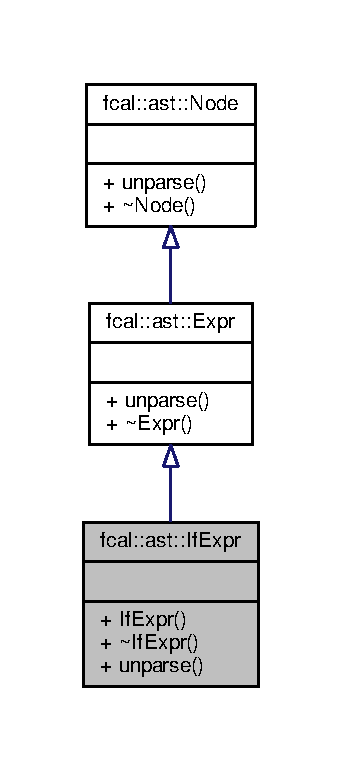
\includegraphics[width=164pt]{classfcal_1_1ast_1_1IfExpr__inherit__graph}
\end{center}
\end{figure}


Collaboration diagram for fcal\+:\+:ast\+:\+:If\+Expr\+:
\nopagebreak
\begin{figure}[H]
\begin{center}
\leavevmode
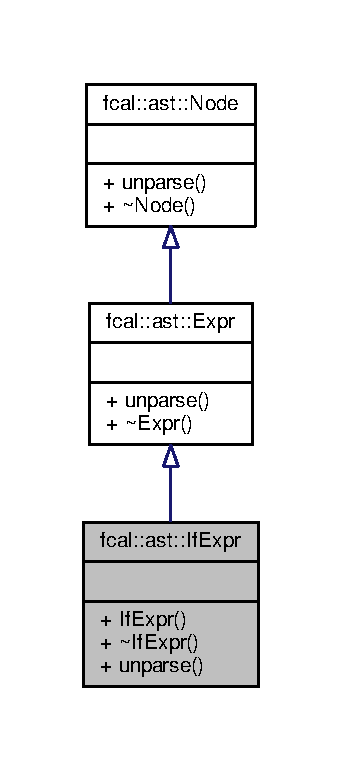
\includegraphics[width=164pt]{classfcal_1_1ast_1_1IfExpr__coll__graph}
\end{center}
\end{figure}
\subsection*{Public Member Functions}
\begin{DoxyCompactItemize}
\item 
\hyperlink{classfcal_1_1ast_1_1IfExpr_ae0ef7ebf56856f692bbd00cb9a226a26}{If\+Expr} (\hyperlink{classfcal_1_1ast_1_1Expr}{Expr} $\ast$e1, \hyperlink{classfcal_1_1ast_1_1Expr}{Expr} $\ast$e2, \hyperlink{classfcal_1_1ast_1_1Expr}{Expr} $\ast$e3)
\item 
\hyperlink{classfcal_1_1ast_1_1IfExpr_abde8683dfdd858d2f3630f5a13e2f345}{$\sim$\+If\+Expr} ()
\item 
std\+::string \hyperlink{classfcal_1_1ast_1_1IfExpr_a4092cf20150a2cde02364d4c7233e558}{unparse} ()
\end{DoxyCompactItemize}


\subsection{Constructor \& Destructor Documentation}
\index{fcal\+::ast\+::\+If\+Expr@{fcal\+::ast\+::\+If\+Expr}!If\+Expr@{If\+Expr}}
\index{If\+Expr@{If\+Expr}!fcal\+::ast\+::\+If\+Expr@{fcal\+::ast\+::\+If\+Expr}}
\subsubsection[{\texorpdfstring{If\+Expr(\+Expr $\ast$e1, Expr $\ast$e2, Expr $\ast$e3)}{IfExpr(Expr *e1, Expr *e2, Expr *e3)}}]{\setlength{\rightskip}{0pt plus 5cm}fcal\+::ast\+::\+If\+Expr\+::\+If\+Expr (
\begin{DoxyParamCaption}
\item[{{\bf Expr} $\ast$}]{e1, }
\item[{{\bf Expr} $\ast$}]{e2, }
\item[{{\bf Expr} $\ast$}]{e3}
\end{DoxyParamCaption}
)\hspace{0.3cm}{\ttfamily [inline]}}\hypertarget{classfcal_1_1ast_1_1IfExpr_ae0ef7ebf56856f692bbd00cb9a226a26}{}\label{classfcal_1_1ast_1_1IfExpr_ae0ef7ebf56856f692bbd00cb9a226a26}
\index{fcal\+::ast\+::\+If\+Expr@{fcal\+::ast\+::\+If\+Expr}!````~If\+Expr@{$\sim$\+If\+Expr}}
\index{````~If\+Expr@{$\sim$\+If\+Expr}!fcal\+::ast\+::\+If\+Expr@{fcal\+::ast\+::\+If\+Expr}}
\subsubsection[{\texorpdfstring{$\sim$\+If\+Expr()}{~IfExpr()}}]{\setlength{\rightskip}{0pt plus 5cm}fcal\+::ast\+::\+If\+Expr\+::$\sim$\+If\+Expr (
\begin{DoxyParamCaption}
{}
\end{DoxyParamCaption}
)\hspace{0.3cm}{\ttfamily [inline]}}\hypertarget{classfcal_1_1ast_1_1IfExpr_abde8683dfdd858d2f3630f5a13e2f345}{}\label{classfcal_1_1ast_1_1IfExpr_abde8683dfdd858d2f3630f5a13e2f345}


\subsection{Member Function Documentation}
\index{fcal\+::ast\+::\+If\+Expr@{fcal\+::ast\+::\+If\+Expr}!unparse@{unparse}}
\index{unparse@{unparse}!fcal\+::ast\+::\+If\+Expr@{fcal\+::ast\+::\+If\+Expr}}
\subsubsection[{\texorpdfstring{unparse()}{unparse()}}]{\setlength{\rightskip}{0pt plus 5cm}std\+::string fcal\+::ast\+::\+If\+Expr\+::unparse (
\begin{DoxyParamCaption}
{}
\end{DoxyParamCaption}
)\hspace{0.3cm}{\ttfamily [inline]}, {\ttfamily [virtual]}}\hypertarget{classfcal_1_1ast_1_1IfExpr_a4092cf20150a2cde02364d4c7233e558}{}\label{classfcal_1_1ast_1_1IfExpr_a4092cf20150a2cde02364d4c7233e558}


Implements \hyperlink{classfcal_1_1ast_1_1Expr_adba9309749d00e7c864456fbd505f252}{fcal\+::ast\+::\+Expr}.



The documentation for this class was generated from the following file\+:\begin{DoxyCompactItemize}
\item 
include/\hyperlink{ast_8h}{ast.\+h}\end{DoxyCompactItemize}

\hypertarget{classfcal_1_1ast_1_1IfStmt}{}\section{fcal\+:\+:ast\+:\+:If\+Stmt Class Reference}
\label{classfcal_1_1ast_1_1IfStmt}\index{fcal\+::ast\+::\+If\+Stmt@{fcal\+::ast\+::\+If\+Stmt}}


{\ttfamily \#include $<$ast.\+h$>$}



Inheritance diagram for fcal\+:\+:ast\+:\+:If\+Stmt\+:
\nopagebreak
\begin{figure}[H]
\begin{center}
\leavevmode
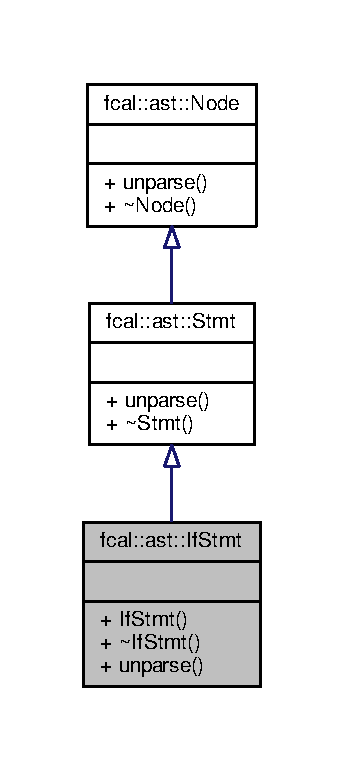
\includegraphics[width=165pt]{classfcal_1_1ast_1_1IfStmt__inherit__graph}
\end{center}
\end{figure}


Collaboration diagram for fcal\+:\+:ast\+:\+:If\+Stmt\+:
\nopagebreak
\begin{figure}[H]
\begin{center}
\leavevmode
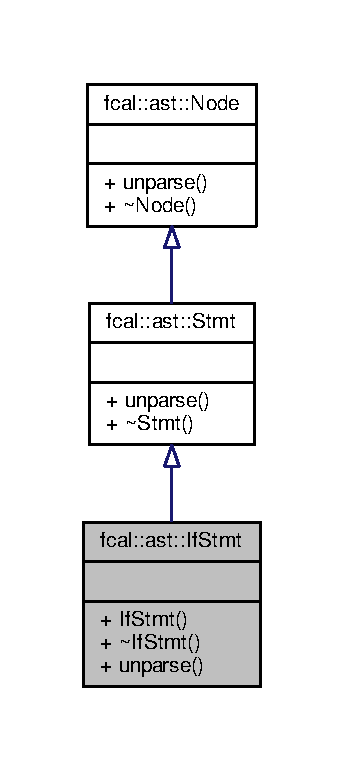
\includegraphics[width=165pt]{classfcal_1_1ast_1_1IfStmt__coll__graph}
\end{center}
\end{figure}
\subsection*{Public Member Functions}
\begin{DoxyCompactItemize}
\item 
\hyperlink{classfcal_1_1ast_1_1IfStmt_a3f91ac7fda63ae79747f5e323c313cc0}{If\+Stmt} (\hyperlink{classfcal_1_1ast_1_1Expr}{Expr} $\ast$e, \hyperlink{classfcal_1_1ast_1_1Stmt}{Stmt} $\ast$s)
\item 
\hyperlink{classfcal_1_1ast_1_1IfStmt_a71d8b2cac8904cde52e99c81ad23ae6f}{$\sim$\+If\+Stmt} ()
\item 
std\+::string \hyperlink{classfcal_1_1ast_1_1IfStmt_acf7d0fbe7a9ff597216a23992f603062}{unparse} ()
\end{DoxyCompactItemize}


\subsection{Constructor \& Destructor Documentation}
\index{fcal\+::ast\+::\+If\+Stmt@{fcal\+::ast\+::\+If\+Stmt}!If\+Stmt@{If\+Stmt}}
\index{If\+Stmt@{If\+Stmt}!fcal\+::ast\+::\+If\+Stmt@{fcal\+::ast\+::\+If\+Stmt}}
\subsubsection[{\texorpdfstring{If\+Stmt(\+Expr $\ast$e, Stmt $\ast$s)}{IfStmt(Expr *e, Stmt *s)}}]{\setlength{\rightskip}{0pt plus 5cm}fcal\+::ast\+::\+If\+Stmt\+::\+If\+Stmt (
\begin{DoxyParamCaption}
\item[{{\bf Expr} $\ast$}]{e, }
\item[{{\bf Stmt} $\ast$}]{s}
\end{DoxyParamCaption}
)\hspace{0.3cm}{\ttfamily [inline]}}\hypertarget{classfcal_1_1ast_1_1IfStmt_a3f91ac7fda63ae79747f5e323c313cc0}{}\label{classfcal_1_1ast_1_1IfStmt_a3f91ac7fda63ae79747f5e323c313cc0}
\index{fcal\+::ast\+::\+If\+Stmt@{fcal\+::ast\+::\+If\+Stmt}!````~If\+Stmt@{$\sim$\+If\+Stmt}}
\index{````~If\+Stmt@{$\sim$\+If\+Stmt}!fcal\+::ast\+::\+If\+Stmt@{fcal\+::ast\+::\+If\+Stmt}}
\subsubsection[{\texorpdfstring{$\sim$\+If\+Stmt()}{~IfStmt()}}]{\setlength{\rightskip}{0pt plus 5cm}fcal\+::ast\+::\+If\+Stmt\+::$\sim$\+If\+Stmt (
\begin{DoxyParamCaption}
{}
\end{DoxyParamCaption}
)\hspace{0.3cm}{\ttfamily [inline]}}\hypertarget{classfcal_1_1ast_1_1IfStmt_a71d8b2cac8904cde52e99c81ad23ae6f}{}\label{classfcal_1_1ast_1_1IfStmt_a71d8b2cac8904cde52e99c81ad23ae6f}


\subsection{Member Function Documentation}
\index{fcal\+::ast\+::\+If\+Stmt@{fcal\+::ast\+::\+If\+Stmt}!unparse@{unparse}}
\index{unparse@{unparse}!fcal\+::ast\+::\+If\+Stmt@{fcal\+::ast\+::\+If\+Stmt}}
\subsubsection[{\texorpdfstring{unparse()}{unparse()}}]{\setlength{\rightskip}{0pt plus 5cm}std\+::string fcal\+::ast\+::\+If\+Stmt\+::unparse (
\begin{DoxyParamCaption}
{}
\end{DoxyParamCaption}
)\hspace{0.3cm}{\ttfamily [inline]}, {\ttfamily [virtual]}}\hypertarget{classfcal_1_1ast_1_1IfStmt_acf7d0fbe7a9ff597216a23992f603062}{}\label{classfcal_1_1ast_1_1IfStmt_acf7d0fbe7a9ff597216a23992f603062}


Implements \hyperlink{classfcal_1_1ast_1_1Stmt_a2ed8595941ddc947012bfeae54f4447d}{fcal\+::ast\+::\+Stmt}.



The documentation for this class was generated from the following file\+:\begin{DoxyCompactItemize}
\item 
include/\hyperlink{ast_8h}{ast.\+h}\end{DoxyCompactItemize}

\hypertarget{classfcal_1_1scanner_1_1IfToken}{}\section{fcal\+:\+:scanner\+:\+:If\+Token Class Reference}
\label{classfcal_1_1scanner_1_1IfToken}\index{fcal\+::scanner\+::\+If\+Token@{fcal\+::scanner\+::\+If\+Token}}


{\ttfamily \#include $<$ext\+\_\+token.\+h$>$}



Inheritance diagram for fcal\+:\+:scanner\+:\+:If\+Token\+:
\nopagebreak
\begin{figure}[H]
\begin{center}
\leavevmode
\includegraphics[width=201pt]{classfcal_1_1scanner_1_1IfToken__inherit__graph}
\end{center}
\end{figure}


Collaboration diagram for fcal\+:\+:scanner\+:\+:If\+Token\+:
\nopagebreak
\begin{figure}[H]
\begin{center}
\leavevmode
\includegraphics[width=201pt]{classfcal_1_1scanner_1_1IfToken__coll__graph}
\end{center}
\end{figure}
\subsection*{Public Member Functions}
\begin{DoxyCompactItemize}
\item 
\hyperlink{classfcal_1_1scanner_1_1IfToken_ab62190e056e132f94f99077fd48049fc}{If\+Token} (\hyperlink{classfcal_1_1parser_1_1Parser}{parser\+::\+Parser} $\ast$p, \hyperlink{classfcal_1_1scanner_1_1Token}{Token} $\ast$t)
\item 
\hyperlink{classfcal_1_1parser_1_1ParseResult}{parser\+::\+Parse\+Result} \hyperlink{classfcal_1_1scanner_1_1IfToken_a66e666cbade5d1be24d0639dad88a594}{nud} ()
\item 
std\+::string \hyperlink{classfcal_1_1scanner_1_1IfToken_a76c60330e996fab7bbcaaab1f825d62c}{description} ()
\item 
int \hyperlink{classfcal_1_1scanner_1_1IfToken_a8ef9ce247acf496793ef3cecafea1c42}{lbp} ()
\end{DoxyCompactItemize}
\subsection*{Additional Inherited Members}


\subsection{Constructor \& Destructor Documentation}
\index{fcal\+::scanner\+::\+If\+Token@{fcal\+::scanner\+::\+If\+Token}!If\+Token@{If\+Token}}
\index{If\+Token@{If\+Token}!fcal\+::scanner\+::\+If\+Token@{fcal\+::scanner\+::\+If\+Token}}
\subsubsection[{\texorpdfstring{If\+Token(parser\+::\+Parser $\ast$p, Token $\ast$t)}{IfToken(parser::Parser *p, Token *t)}}]{\setlength{\rightskip}{0pt plus 5cm}fcal\+::scanner\+::\+If\+Token\+::\+If\+Token (
\begin{DoxyParamCaption}
\item[{{\bf parser\+::\+Parser} $\ast$}]{p, }
\item[{{\bf Token} $\ast$}]{t}
\end{DoxyParamCaption}
)\hspace{0.3cm}{\ttfamily [inline]}}\hypertarget{classfcal_1_1scanner_1_1IfToken_ab62190e056e132f94f99077fd48049fc}{}\label{classfcal_1_1scanner_1_1IfToken_ab62190e056e132f94f99077fd48049fc}


\subsection{Member Function Documentation}
\index{fcal\+::scanner\+::\+If\+Token@{fcal\+::scanner\+::\+If\+Token}!description@{description}}
\index{description@{description}!fcal\+::scanner\+::\+If\+Token@{fcal\+::scanner\+::\+If\+Token}}
\subsubsection[{\texorpdfstring{description()}{description()}}]{\setlength{\rightskip}{0pt plus 5cm}std\+::string fcal\+::scanner\+::\+If\+Token\+::description (
\begin{DoxyParamCaption}
{}
\end{DoxyParamCaption}
)\hspace{0.3cm}{\ttfamily [inline]}, {\ttfamily [virtual]}}\hypertarget{classfcal_1_1scanner_1_1IfToken_a76c60330e996fab7bbcaaab1f825d62c}{}\label{classfcal_1_1scanner_1_1IfToken_a76c60330e996fab7bbcaaab1f825d62c}


Reimplemented from \hyperlink{classfcal_1_1scanner_1_1ExtToken_a29a72149492d7fef7968a1b894d334c7}{fcal\+::scanner\+::\+Ext\+Token}.

\index{fcal\+::scanner\+::\+If\+Token@{fcal\+::scanner\+::\+If\+Token}!lbp@{lbp}}
\index{lbp@{lbp}!fcal\+::scanner\+::\+If\+Token@{fcal\+::scanner\+::\+If\+Token}}
\subsubsection[{\texorpdfstring{lbp()}{lbp()}}]{\setlength{\rightskip}{0pt plus 5cm}int fcal\+::scanner\+::\+If\+Token\+::lbp (
\begin{DoxyParamCaption}
{}
\end{DoxyParamCaption}
)\hspace{0.3cm}{\ttfamily [inline]}, {\ttfamily [virtual]}}\hypertarget{classfcal_1_1scanner_1_1IfToken_a8ef9ce247acf496793ef3cecafea1c42}{}\label{classfcal_1_1scanner_1_1IfToken_a8ef9ce247acf496793ef3cecafea1c42}


Reimplemented from \hyperlink{classfcal_1_1scanner_1_1ExtToken_adecef3770f08e5a26f103ab62171cc91}{fcal\+::scanner\+::\+Ext\+Token}.

\index{fcal\+::scanner\+::\+If\+Token@{fcal\+::scanner\+::\+If\+Token}!nud@{nud}}
\index{nud@{nud}!fcal\+::scanner\+::\+If\+Token@{fcal\+::scanner\+::\+If\+Token}}
\subsubsection[{\texorpdfstring{nud()}{nud()}}]{\setlength{\rightskip}{0pt plus 5cm}{\bf parser\+::\+Parse\+Result} fcal\+::scanner\+::\+If\+Token\+::nud (
\begin{DoxyParamCaption}
\item[{void}]{}
\end{DoxyParamCaption}
)\hspace{0.3cm}{\ttfamily [inline]}, {\ttfamily [virtual]}}\hypertarget{classfcal_1_1scanner_1_1IfToken_a66e666cbade5d1be24d0639dad88a594}{}\label{classfcal_1_1scanner_1_1IfToken_a66e666cbade5d1be24d0639dad88a594}


Reimplemented from \hyperlink{classfcal_1_1scanner_1_1ExtToken_a2e1ca27a07d55593ffd67780dbcad7dd}{fcal\+::scanner\+::\+Ext\+Token}.



The documentation for this class was generated from the following file\+:\begin{DoxyCompactItemize}
\item 
include/\hyperlink{ext__token_8h}{ext\+\_\+token.\+h}\end{DoxyCompactItemize}

\hypertarget{classfcal_1_1scanner_1_1IntConstToken}{}\section{fcal\+:\+:scanner\+:\+:Int\+Const\+Token Class Reference}
\label{classfcal_1_1scanner_1_1IntConstToken}\index{fcal\+::scanner\+::\+Int\+Const\+Token@{fcal\+::scanner\+::\+Int\+Const\+Token}}


{\ttfamily \#include $<$ext\+\_\+token.\+h$>$}



Inheritance diagram for fcal\+:\+:scanner\+:\+:Int\+Const\+Token\+:
\nopagebreak
\begin{figure}[H]
\begin{center}
\leavevmode
\includegraphics[width=223pt]{classfcal_1_1scanner_1_1IntConstToken__inherit__graph}
\end{center}
\end{figure}


Collaboration diagram for fcal\+:\+:scanner\+:\+:Int\+Const\+Token\+:
\nopagebreak
\begin{figure}[H]
\begin{center}
\leavevmode
\includegraphics[width=223pt]{classfcal_1_1scanner_1_1IntConstToken__coll__graph}
\end{center}
\end{figure}
\subsection*{Public Member Functions}
\begin{DoxyCompactItemize}
\item 
\hyperlink{classfcal_1_1scanner_1_1IntConstToken_a2846b99b9b48717e35d81446618eb924}{Int\+Const\+Token} (\hyperlink{classfcal_1_1parser_1_1Parser}{parser\+::\+Parser} $\ast$p, \hyperlink{classfcal_1_1scanner_1_1Token}{Token} $\ast$t)
\item 
\hyperlink{classfcal_1_1parser_1_1ParseResult}{parser\+::\+Parse\+Result} \hyperlink{classfcal_1_1scanner_1_1IntConstToken_aede9ed23780dbb33a7852b3ecf6183da}{nud} ()
\item 
std\+::string \hyperlink{classfcal_1_1scanner_1_1IntConstToken_a9359c997cac9cf57a5c7debc6a1811ab}{description} ()
\end{DoxyCompactItemize}
\subsection*{Additional Inherited Members}


\subsection{Constructor \& Destructor Documentation}
\index{fcal\+::scanner\+::\+Int\+Const\+Token@{fcal\+::scanner\+::\+Int\+Const\+Token}!Int\+Const\+Token@{Int\+Const\+Token}}
\index{Int\+Const\+Token@{Int\+Const\+Token}!fcal\+::scanner\+::\+Int\+Const\+Token@{fcal\+::scanner\+::\+Int\+Const\+Token}}
\subsubsection[{\texorpdfstring{Int\+Const\+Token(parser\+::\+Parser $\ast$p, Token $\ast$t)}{IntConstToken(parser::Parser *p, Token *t)}}]{\setlength{\rightskip}{0pt plus 5cm}fcal\+::scanner\+::\+Int\+Const\+Token\+::\+Int\+Const\+Token (
\begin{DoxyParamCaption}
\item[{{\bf parser\+::\+Parser} $\ast$}]{p, }
\item[{{\bf Token} $\ast$}]{t}
\end{DoxyParamCaption}
)\hspace{0.3cm}{\ttfamily [inline]}}\hypertarget{classfcal_1_1scanner_1_1IntConstToken_a2846b99b9b48717e35d81446618eb924}{}\label{classfcal_1_1scanner_1_1IntConstToken_a2846b99b9b48717e35d81446618eb924}


\subsection{Member Function Documentation}
\index{fcal\+::scanner\+::\+Int\+Const\+Token@{fcal\+::scanner\+::\+Int\+Const\+Token}!description@{description}}
\index{description@{description}!fcal\+::scanner\+::\+Int\+Const\+Token@{fcal\+::scanner\+::\+Int\+Const\+Token}}
\subsubsection[{\texorpdfstring{description()}{description()}}]{\setlength{\rightskip}{0pt plus 5cm}std\+::string fcal\+::scanner\+::\+Int\+Const\+Token\+::description (
\begin{DoxyParamCaption}
{}
\end{DoxyParamCaption}
)\hspace{0.3cm}{\ttfamily [inline]}, {\ttfamily [virtual]}}\hypertarget{classfcal_1_1scanner_1_1IntConstToken_a9359c997cac9cf57a5c7debc6a1811ab}{}\label{classfcal_1_1scanner_1_1IntConstToken_a9359c997cac9cf57a5c7debc6a1811ab}


Reimplemented from \hyperlink{classfcal_1_1scanner_1_1ExtToken_a29a72149492d7fef7968a1b894d334c7}{fcal\+::scanner\+::\+Ext\+Token}.

\index{fcal\+::scanner\+::\+Int\+Const\+Token@{fcal\+::scanner\+::\+Int\+Const\+Token}!nud@{nud}}
\index{nud@{nud}!fcal\+::scanner\+::\+Int\+Const\+Token@{fcal\+::scanner\+::\+Int\+Const\+Token}}
\subsubsection[{\texorpdfstring{nud()}{nud()}}]{\setlength{\rightskip}{0pt plus 5cm}{\bf parser\+::\+Parse\+Result} fcal\+::scanner\+::\+Int\+Const\+Token\+::nud (
\begin{DoxyParamCaption}
\item[{void}]{}
\end{DoxyParamCaption}
)\hspace{0.3cm}{\ttfamily [inline]}, {\ttfamily [virtual]}}\hypertarget{classfcal_1_1scanner_1_1IntConstToken_aede9ed23780dbb33a7852b3ecf6183da}{}\label{classfcal_1_1scanner_1_1IntConstToken_aede9ed23780dbb33a7852b3ecf6183da}


Reimplemented from \hyperlink{classfcal_1_1scanner_1_1ExtToken_a2e1ca27a07d55593ffd67780dbcad7dd}{fcal\+::scanner\+::\+Ext\+Token}.



The documentation for this class was generated from the following file\+:\begin{DoxyCompactItemize}
\item 
include/\hyperlink{ext__token_8h}{ext\+\_\+token.\+h}\end{DoxyCompactItemize}

\hypertarget{classfcal_1_1ast_1_1IntDecl}{}\section{fcal\+:\+:ast\+:\+:Int\+Decl Class Reference}
\label{classfcal_1_1ast_1_1IntDecl}\index{fcal\+::ast\+::\+Int\+Decl@{fcal\+::ast\+::\+Int\+Decl}}


{\ttfamily \#include $<$ast.\+h$>$}



Inheritance diagram for fcal\+:\+:ast\+:\+:Int\+Decl\+:
\nopagebreak
\begin{figure}[H]
\begin{center}
\leavevmode
\includegraphics[width=169pt]{classfcal_1_1ast_1_1IntDecl__inherit__graph}
\end{center}
\end{figure}


Collaboration diagram for fcal\+:\+:ast\+:\+:Int\+Decl\+:
\nopagebreak
\begin{figure}[H]
\begin{center}
\leavevmode
\includegraphics[width=169pt]{classfcal_1_1ast_1_1IntDecl__coll__graph}
\end{center}
\end{figure}
\subsection*{Public Member Functions}
\begin{DoxyCompactItemize}
\item 
\hyperlink{classfcal_1_1ast_1_1IntDecl_a2b6be0e39a793d86f71fe429b1a46f12}{Int\+Decl} (std\+::string s)
\item 
\hyperlink{classfcal_1_1ast_1_1IntDecl_a44b8a580dddc86a9bc10052d5a4ac275}{$\sim$\+Int\+Decl} ()
\item 
std\+::string \hyperlink{classfcal_1_1ast_1_1IntDecl_a70cae495e6036b864fb6750cb9acac19}{unparse} ()
\end{DoxyCompactItemize}


\subsection{Detailed Description}
The following classes directly inherit from the virtual \hyperlink{classfcal_1_1ast_1_1Decl}{Decl} class. These classes provide constructors for declarations based on the F\+C\+AL grammar. 

\subsection{Constructor \& Destructor Documentation}
\index{fcal\+::ast\+::\+Int\+Decl@{fcal\+::ast\+::\+Int\+Decl}!Int\+Decl@{Int\+Decl}}
\index{Int\+Decl@{Int\+Decl}!fcal\+::ast\+::\+Int\+Decl@{fcal\+::ast\+::\+Int\+Decl}}
\subsubsection[{\texorpdfstring{Int\+Decl(std\+::string s)}{IntDecl(std::string s)}}]{\setlength{\rightskip}{0pt plus 5cm}fcal\+::ast\+::\+Int\+Decl\+::\+Int\+Decl (
\begin{DoxyParamCaption}
\item[{std\+::string}]{s}
\end{DoxyParamCaption}
)\hspace{0.3cm}{\ttfamily [inline]}, {\ttfamily [explicit]}}\hypertarget{classfcal_1_1ast_1_1IntDecl_a2b6be0e39a793d86f71fe429b1a46f12}{}\label{classfcal_1_1ast_1_1IntDecl_a2b6be0e39a793d86f71fe429b1a46f12}
\index{fcal\+::ast\+::\+Int\+Decl@{fcal\+::ast\+::\+Int\+Decl}!````~Int\+Decl@{$\sim$\+Int\+Decl}}
\index{````~Int\+Decl@{$\sim$\+Int\+Decl}!fcal\+::ast\+::\+Int\+Decl@{fcal\+::ast\+::\+Int\+Decl}}
\subsubsection[{\texorpdfstring{$\sim$\+Int\+Decl()}{~IntDecl()}}]{\setlength{\rightskip}{0pt plus 5cm}fcal\+::ast\+::\+Int\+Decl\+::$\sim$\+Int\+Decl (
\begin{DoxyParamCaption}
{}
\end{DoxyParamCaption}
)\hspace{0.3cm}{\ttfamily [inline]}}\hypertarget{classfcal_1_1ast_1_1IntDecl_a44b8a580dddc86a9bc10052d5a4ac275}{}\label{classfcal_1_1ast_1_1IntDecl_a44b8a580dddc86a9bc10052d5a4ac275}


\subsection{Member Function Documentation}
\index{fcal\+::ast\+::\+Int\+Decl@{fcal\+::ast\+::\+Int\+Decl}!unparse@{unparse}}
\index{unparse@{unparse}!fcal\+::ast\+::\+Int\+Decl@{fcal\+::ast\+::\+Int\+Decl}}
\subsubsection[{\texorpdfstring{unparse()}{unparse()}}]{\setlength{\rightskip}{0pt plus 5cm}std\+::string fcal\+::ast\+::\+Int\+Decl\+::unparse (
\begin{DoxyParamCaption}
{}
\end{DoxyParamCaption}
)\hspace{0.3cm}{\ttfamily [inline]}, {\ttfamily [virtual]}}\hypertarget{classfcal_1_1ast_1_1IntDecl_a70cae495e6036b864fb6750cb9acac19}{}\label{classfcal_1_1ast_1_1IntDecl_a70cae495e6036b864fb6750cb9acac19}


Implements \hyperlink{classfcal_1_1ast_1_1Decl_a54761cf8b990cb2d478c606be6bc29c5}{fcal\+::ast\+::\+Decl}.



The documentation for this class was generated from the following file\+:\begin{DoxyCompactItemize}
\item 
include/\hyperlink{ast_8h}{ast.\+h}\end{DoxyCompactItemize}

\hypertarget{classfcal_1_1ast_1_1IntegerConstExpr}{}\section{fcal\+:\+:ast\+:\+:Integer\+Const\+Expr Class Reference}
\label{classfcal_1_1ast_1_1IntegerConstExpr}\index{fcal\+::ast\+::\+Integer\+Const\+Expr@{fcal\+::ast\+::\+Integer\+Const\+Expr}}


{\ttfamily \#include $<$ast.\+h$>$}



Inheritance diagram for fcal\+:\+:ast\+:\+:Integer\+Const\+Expr\+:
\nopagebreak
\begin{figure}[H]
\begin{center}
\leavevmode
\includegraphics[width=214pt]{classfcal_1_1ast_1_1IntegerConstExpr__inherit__graph}
\end{center}
\end{figure}


Collaboration diagram for fcal\+:\+:ast\+:\+:Integer\+Const\+Expr\+:
\nopagebreak
\begin{figure}[H]
\begin{center}
\leavevmode
\includegraphics[width=214pt]{classfcal_1_1ast_1_1IntegerConstExpr__coll__graph}
\end{center}
\end{figure}
\subsection*{Public Member Functions}
\begin{DoxyCompactItemize}
\item 
\hyperlink{classfcal_1_1ast_1_1IntegerConstExpr_a91327bb29876851e171ae1d8579de88f}{Integer\+Const\+Expr} (std\+::string i)
\item 
\hyperlink{classfcal_1_1ast_1_1IntegerConstExpr_a1aa3a4a6f88a68af7f8acf126f766369}{$\sim$\+Integer\+Const\+Expr} ()
\item 
std\+::string \hyperlink{classfcal_1_1ast_1_1IntegerConstExpr_afccb833ff588cd49929358ab76cafdc4}{unparse} ()
\end{DoxyCompactItemize}


\subsection{Constructor \& Destructor Documentation}
\index{fcal\+::ast\+::\+Integer\+Const\+Expr@{fcal\+::ast\+::\+Integer\+Const\+Expr}!Integer\+Const\+Expr@{Integer\+Const\+Expr}}
\index{Integer\+Const\+Expr@{Integer\+Const\+Expr}!fcal\+::ast\+::\+Integer\+Const\+Expr@{fcal\+::ast\+::\+Integer\+Const\+Expr}}
\subsubsection[{\texorpdfstring{Integer\+Const\+Expr(std\+::string i)}{IntegerConstExpr(std::string i)}}]{\setlength{\rightskip}{0pt plus 5cm}fcal\+::ast\+::\+Integer\+Const\+Expr\+::\+Integer\+Const\+Expr (
\begin{DoxyParamCaption}
\item[{std\+::string}]{i}
\end{DoxyParamCaption}
)\hspace{0.3cm}{\ttfamily [inline]}, {\ttfamily [explicit]}}\hypertarget{classfcal_1_1ast_1_1IntegerConstExpr_a91327bb29876851e171ae1d8579de88f}{}\label{classfcal_1_1ast_1_1IntegerConstExpr_a91327bb29876851e171ae1d8579de88f}
\index{fcal\+::ast\+::\+Integer\+Const\+Expr@{fcal\+::ast\+::\+Integer\+Const\+Expr}!````~Integer\+Const\+Expr@{$\sim$\+Integer\+Const\+Expr}}
\index{````~Integer\+Const\+Expr@{$\sim$\+Integer\+Const\+Expr}!fcal\+::ast\+::\+Integer\+Const\+Expr@{fcal\+::ast\+::\+Integer\+Const\+Expr}}
\subsubsection[{\texorpdfstring{$\sim$\+Integer\+Const\+Expr()}{~IntegerConstExpr()}}]{\setlength{\rightskip}{0pt plus 5cm}fcal\+::ast\+::\+Integer\+Const\+Expr\+::$\sim$\+Integer\+Const\+Expr (
\begin{DoxyParamCaption}
{}
\end{DoxyParamCaption}
)\hspace{0.3cm}{\ttfamily [inline]}}\hypertarget{classfcal_1_1ast_1_1IntegerConstExpr_a1aa3a4a6f88a68af7f8acf126f766369}{}\label{classfcal_1_1ast_1_1IntegerConstExpr_a1aa3a4a6f88a68af7f8acf126f766369}


\subsection{Member Function Documentation}
\index{fcal\+::ast\+::\+Integer\+Const\+Expr@{fcal\+::ast\+::\+Integer\+Const\+Expr}!unparse@{unparse}}
\index{unparse@{unparse}!fcal\+::ast\+::\+Integer\+Const\+Expr@{fcal\+::ast\+::\+Integer\+Const\+Expr}}
\subsubsection[{\texorpdfstring{unparse()}{unparse()}}]{\setlength{\rightskip}{0pt plus 5cm}std\+::string fcal\+::ast\+::\+Integer\+Const\+Expr\+::unparse (
\begin{DoxyParamCaption}
{}
\end{DoxyParamCaption}
)\hspace{0.3cm}{\ttfamily [inline]}, {\ttfamily [virtual]}}\hypertarget{classfcal_1_1ast_1_1IntegerConstExpr_afccb833ff588cd49929358ab76cafdc4}{}\label{classfcal_1_1ast_1_1IntegerConstExpr_afccb833ff588cd49929358ab76cafdc4}


Implements \hyperlink{classfcal_1_1ast_1_1Expr_adba9309749d00e7c864456fbd505f252}{fcal\+::ast\+::\+Expr}.



The documentation for this class was generated from the following file\+:\begin{DoxyCompactItemize}
\item 
include/\hyperlink{ast_8h}{ast.\+h}\end{DoxyCompactItemize}

\hypertarget{classfcal_1_1scanner_1_1LeftParenToken}{}\section{fcal\+:\+:scanner\+:\+:Left\+Paren\+Token Class Reference}
\label{classfcal_1_1scanner_1_1LeftParenToken}\index{fcal\+::scanner\+::\+Left\+Paren\+Token@{fcal\+::scanner\+::\+Left\+Paren\+Token}}


{\ttfamily \#include $<$ext\+\_\+token.\+h$>$}



Inheritance diagram for fcal\+:\+:scanner\+:\+:Left\+Paren\+Token\+:
\nopagebreak
\begin{figure}[H]
\begin{center}
\leavevmode
\includegraphics[width=201pt]{classfcal_1_1scanner_1_1LeftParenToken__inherit__graph}
\end{center}
\end{figure}


Collaboration diagram for fcal\+:\+:scanner\+:\+:Left\+Paren\+Token\+:
\nopagebreak
\begin{figure}[H]
\begin{center}
\leavevmode
\includegraphics[width=201pt]{classfcal_1_1scanner_1_1LeftParenToken__coll__graph}
\end{center}
\end{figure}
\subsection*{Public Member Functions}
\begin{DoxyCompactItemize}
\item 
\hyperlink{classfcal_1_1scanner_1_1LeftParenToken_a306e81a052bdff9c4e9fb4912e0732ee}{Left\+Paren\+Token} (\hyperlink{classfcal_1_1parser_1_1Parser}{parser\+::\+Parser} $\ast$p, \hyperlink{classfcal_1_1scanner_1_1Token}{Token} $\ast$t)
\item 
\hyperlink{classfcal_1_1parser_1_1ParseResult}{parser\+::\+Parse\+Result} \hyperlink{classfcal_1_1scanner_1_1LeftParenToken_a793eb1dfcd6ea5546081c7cf8733534a}{nud} ()
\item 
std\+::string \hyperlink{classfcal_1_1scanner_1_1LeftParenToken_a32ea8cf7b793bb532161781f8f42113c}{description} ()
\item 
int \hyperlink{classfcal_1_1scanner_1_1LeftParenToken_a2bfc3c31dc0fef8961d4f33a3bc81f25}{lbp} ()
\end{DoxyCompactItemize}
\subsection*{Additional Inherited Members}


\subsection{Constructor \& Destructor Documentation}
\index{fcal\+::scanner\+::\+Left\+Paren\+Token@{fcal\+::scanner\+::\+Left\+Paren\+Token}!Left\+Paren\+Token@{Left\+Paren\+Token}}
\index{Left\+Paren\+Token@{Left\+Paren\+Token}!fcal\+::scanner\+::\+Left\+Paren\+Token@{fcal\+::scanner\+::\+Left\+Paren\+Token}}
\subsubsection[{\texorpdfstring{Left\+Paren\+Token(parser\+::\+Parser $\ast$p, Token $\ast$t)}{LeftParenToken(parser::Parser *p, Token *t)}}]{\setlength{\rightskip}{0pt plus 5cm}fcal\+::scanner\+::\+Left\+Paren\+Token\+::\+Left\+Paren\+Token (
\begin{DoxyParamCaption}
\item[{{\bf parser\+::\+Parser} $\ast$}]{p, }
\item[{{\bf Token} $\ast$}]{t}
\end{DoxyParamCaption}
)\hspace{0.3cm}{\ttfamily [inline]}}\hypertarget{classfcal_1_1scanner_1_1LeftParenToken_a306e81a052bdff9c4e9fb4912e0732ee}{}\label{classfcal_1_1scanner_1_1LeftParenToken_a306e81a052bdff9c4e9fb4912e0732ee}


\subsection{Member Function Documentation}
\index{fcal\+::scanner\+::\+Left\+Paren\+Token@{fcal\+::scanner\+::\+Left\+Paren\+Token}!description@{description}}
\index{description@{description}!fcal\+::scanner\+::\+Left\+Paren\+Token@{fcal\+::scanner\+::\+Left\+Paren\+Token}}
\subsubsection[{\texorpdfstring{description()}{description()}}]{\setlength{\rightskip}{0pt plus 5cm}std\+::string fcal\+::scanner\+::\+Left\+Paren\+Token\+::description (
\begin{DoxyParamCaption}
{}
\end{DoxyParamCaption}
)\hspace{0.3cm}{\ttfamily [inline]}, {\ttfamily [virtual]}}\hypertarget{classfcal_1_1scanner_1_1LeftParenToken_a32ea8cf7b793bb532161781f8f42113c}{}\label{classfcal_1_1scanner_1_1LeftParenToken_a32ea8cf7b793bb532161781f8f42113c}


Reimplemented from \hyperlink{classfcal_1_1scanner_1_1ExtToken_a29a72149492d7fef7968a1b894d334c7}{fcal\+::scanner\+::\+Ext\+Token}.

\index{fcal\+::scanner\+::\+Left\+Paren\+Token@{fcal\+::scanner\+::\+Left\+Paren\+Token}!lbp@{lbp}}
\index{lbp@{lbp}!fcal\+::scanner\+::\+Left\+Paren\+Token@{fcal\+::scanner\+::\+Left\+Paren\+Token}}
\subsubsection[{\texorpdfstring{lbp()}{lbp()}}]{\setlength{\rightskip}{0pt plus 5cm}int fcal\+::scanner\+::\+Left\+Paren\+Token\+::lbp (
\begin{DoxyParamCaption}
{}
\end{DoxyParamCaption}
)\hspace{0.3cm}{\ttfamily [inline]}, {\ttfamily [virtual]}}\hypertarget{classfcal_1_1scanner_1_1LeftParenToken_a2bfc3c31dc0fef8961d4f33a3bc81f25}{}\label{classfcal_1_1scanner_1_1LeftParenToken_a2bfc3c31dc0fef8961d4f33a3bc81f25}


Reimplemented from \hyperlink{classfcal_1_1scanner_1_1ExtToken_adecef3770f08e5a26f103ab62171cc91}{fcal\+::scanner\+::\+Ext\+Token}.

\index{fcal\+::scanner\+::\+Left\+Paren\+Token@{fcal\+::scanner\+::\+Left\+Paren\+Token}!nud@{nud}}
\index{nud@{nud}!fcal\+::scanner\+::\+Left\+Paren\+Token@{fcal\+::scanner\+::\+Left\+Paren\+Token}}
\subsubsection[{\texorpdfstring{nud()}{nud()}}]{\setlength{\rightskip}{0pt plus 5cm}{\bf parser\+::\+Parse\+Result} fcal\+::scanner\+::\+Left\+Paren\+Token\+::nud (
\begin{DoxyParamCaption}
\item[{void}]{}
\end{DoxyParamCaption}
)\hspace{0.3cm}{\ttfamily [inline]}, {\ttfamily [virtual]}}\hypertarget{classfcal_1_1scanner_1_1LeftParenToken_a793eb1dfcd6ea5546081c7cf8733534a}{}\label{classfcal_1_1scanner_1_1LeftParenToken_a793eb1dfcd6ea5546081c7cf8733534a}


Reimplemented from \hyperlink{classfcal_1_1scanner_1_1ExtToken_a2e1ca27a07d55593ffd67780dbcad7dd}{fcal\+::scanner\+::\+Ext\+Token}.



The documentation for this class was generated from the following file\+:\begin{DoxyCompactItemize}
\item 
include/\hyperlink{ext__token_8h}{ext\+\_\+token.\+h}\end{DoxyCompactItemize}

\hypertarget{classfcal_1_1ast_1_1LessEqualExpr}{}\section{fcal\+:\+:ast\+:\+:Less\+Equal\+Expr Class Reference}
\label{classfcal_1_1ast_1_1LessEqualExpr}\index{fcal\+::ast\+::\+Less\+Equal\+Expr@{fcal\+::ast\+::\+Less\+Equal\+Expr}}


{\ttfamily \#include $<$ast.\+h$>$}



Inheritance diagram for fcal\+:\+:ast\+:\+:Less\+Equal\+Expr\+:
\nopagebreak
\begin{figure}[H]
\begin{center}
\leavevmode
\includegraphics[width=204pt]{classfcal_1_1ast_1_1LessEqualExpr__inherit__graph}
\end{center}
\end{figure}


Collaboration diagram for fcal\+:\+:ast\+:\+:Less\+Equal\+Expr\+:
\nopagebreak
\begin{figure}[H]
\begin{center}
\leavevmode
\includegraphics[width=204pt]{classfcal_1_1ast_1_1LessEqualExpr__coll__graph}
\end{center}
\end{figure}
\subsection*{Public Member Functions}
\begin{DoxyCompactItemize}
\item 
\hyperlink{classfcal_1_1ast_1_1LessEqualExpr_af2ed0f19ebe90dad9f09620719ca388f}{Less\+Equal\+Expr} (\hyperlink{classfcal_1_1ast_1_1Expr}{Expr} $\ast$e1, \hyperlink{classfcal_1_1ast_1_1Expr}{Expr} $\ast$e2)
\item 
\hyperlink{classfcal_1_1ast_1_1LessEqualExpr_a33d3a192e3fc66006ec313ad54dfe2de}{$\sim$\+Less\+Equal\+Expr} ()
\item 
std\+::string \hyperlink{classfcal_1_1ast_1_1LessEqualExpr_a78181c2bc69a185d97753d23c823b6a0}{unparse} ()
\end{DoxyCompactItemize}


\subsection{Constructor \& Destructor Documentation}
\index{fcal\+::ast\+::\+Less\+Equal\+Expr@{fcal\+::ast\+::\+Less\+Equal\+Expr}!Less\+Equal\+Expr@{Less\+Equal\+Expr}}
\index{Less\+Equal\+Expr@{Less\+Equal\+Expr}!fcal\+::ast\+::\+Less\+Equal\+Expr@{fcal\+::ast\+::\+Less\+Equal\+Expr}}
\subsubsection[{\texorpdfstring{Less\+Equal\+Expr(\+Expr $\ast$e1, Expr $\ast$e2)}{LessEqualExpr(Expr *e1, Expr *e2)}}]{\setlength{\rightskip}{0pt plus 5cm}fcal\+::ast\+::\+Less\+Equal\+Expr\+::\+Less\+Equal\+Expr (
\begin{DoxyParamCaption}
\item[{{\bf Expr} $\ast$}]{e1, }
\item[{{\bf Expr} $\ast$}]{e2}
\end{DoxyParamCaption}
)\hspace{0.3cm}{\ttfamily [inline]}}\hypertarget{classfcal_1_1ast_1_1LessEqualExpr_af2ed0f19ebe90dad9f09620719ca388f}{}\label{classfcal_1_1ast_1_1LessEqualExpr_af2ed0f19ebe90dad9f09620719ca388f}
\index{fcal\+::ast\+::\+Less\+Equal\+Expr@{fcal\+::ast\+::\+Less\+Equal\+Expr}!````~Less\+Equal\+Expr@{$\sim$\+Less\+Equal\+Expr}}
\index{````~Less\+Equal\+Expr@{$\sim$\+Less\+Equal\+Expr}!fcal\+::ast\+::\+Less\+Equal\+Expr@{fcal\+::ast\+::\+Less\+Equal\+Expr}}
\subsubsection[{\texorpdfstring{$\sim$\+Less\+Equal\+Expr()}{~LessEqualExpr()}}]{\setlength{\rightskip}{0pt plus 5cm}fcal\+::ast\+::\+Less\+Equal\+Expr\+::$\sim$\+Less\+Equal\+Expr (
\begin{DoxyParamCaption}
{}
\end{DoxyParamCaption}
)\hspace{0.3cm}{\ttfamily [inline]}}\hypertarget{classfcal_1_1ast_1_1LessEqualExpr_a33d3a192e3fc66006ec313ad54dfe2de}{}\label{classfcal_1_1ast_1_1LessEqualExpr_a33d3a192e3fc66006ec313ad54dfe2de}


\subsection{Member Function Documentation}
\index{fcal\+::ast\+::\+Less\+Equal\+Expr@{fcal\+::ast\+::\+Less\+Equal\+Expr}!unparse@{unparse}}
\index{unparse@{unparse}!fcal\+::ast\+::\+Less\+Equal\+Expr@{fcal\+::ast\+::\+Less\+Equal\+Expr}}
\subsubsection[{\texorpdfstring{unparse()}{unparse()}}]{\setlength{\rightskip}{0pt plus 5cm}std\+::string fcal\+::ast\+::\+Less\+Equal\+Expr\+::unparse (
\begin{DoxyParamCaption}
{}
\end{DoxyParamCaption}
)\hspace{0.3cm}{\ttfamily [inline]}, {\ttfamily [virtual]}}\hypertarget{classfcal_1_1ast_1_1LessEqualExpr_a78181c2bc69a185d97753d23c823b6a0}{}\label{classfcal_1_1ast_1_1LessEqualExpr_a78181c2bc69a185d97753d23c823b6a0}


Implements \hyperlink{classfcal_1_1ast_1_1Expr_adba9309749d00e7c864456fbd505f252}{fcal\+::ast\+::\+Expr}.



The documentation for this class was generated from the following file\+:\begin{DoxyCompactItemize}
\item 
include/\hyperlink{ast_8h}{ast.\+h}\end{DoxyCompactItemize}

\hypertarget{classfcal_1_1ast_1_1LessExpr}{}\section{fcal\+:\+:ast\+:\+:Less\+Expr Class Reference}
\label{classfcal_1_1ast_1_1LessExpr}\index{fcal\+::ast\+::\+Less\+Expr@{fcal\+::ast\+::\+Less\+Expr}}


{\ttfamily \#include $<$ast.\+h$>$}



Inheritance diagram for fcal\+:\+:ast\+:\+:Less\+Expr\+:
\nopagebreak
\begin{figure}[H]
\begin{center}
\leavevmode
\includegraphics[width=179pt]{classfcal_1_1ast_1_1LessExpr__inherit__graph}
\end{center}
\end{figure}


Collaboration diagram for fcal\+:\+:ast\+:\+:Less\+Expr\+:
\nopagebreak
\begin{figure}[H]
\begin{center}
\leavevmode
\includegraphics[width=179pt]{classfcal_1_1ast_1_1LessExpr__coll__graph}
\end{center}
\end{figure}
\subsection*{Public Member Functions}
\begin{DoxyCompactItemize}
\item 
\hyperlink{classfcal_1_1ast_1_1LessExpr_a01e38dff197780fd0ae1ee75afcd89dc}{Less\+Expr} (\hyperlink{classfcal_1_1ast_1_1Expr}{Expr} $\ast$e1, \hyperlink{classfcal_1_1ast_1_1Expr}{Expr} $\ast$e2)
\item 
\hyperlink{classfcal_1_1ast_1_1LessExpr_af5f22e3a2e2ebe7bb9c22638ce001583}{$\sim$\+Less\+Expr} ()
\item 
std\+::string \hyperlink{classfcal_1_1ast_1_1LessExpr_af3a7eb1f384374183b28ca01224827e2}{unparse} ()
\end{DoxyCompactItemize}


\subsection{Constructor \& Destructor Documentation}
\index{fcal\+::ast\+::\+Less\+Expr@{fcal\+::ast\+::\+Less\+Expr}!Less\+Expr@{Less\+Expr}}
\index{Less\+Expr@{Less\+Expr}!fcal\+::ast\+::\+Less\+Expr@{fcal\+::ast\+::\+Less\+Expr}}
\subsubsection[{\texorpdfstring{Less\+Expr(\+Expr $\ast$e1, Expr $\ast$e2)}{LessExpr(Expr *e1, Expr *e2)}}]{\setlength{\rightskip}{0pt plus 5cm}fcal\+::ast\+::\+Less\+Expr\+::\+Less\+Expr (
\begin{DoxyParamCaption}
\item[{{\bf Expr} $\ast$}]{e1, }
\item[{{\bf Expr} $\ast$}]{e2}
\end{DoxyParamCaption}
)\hspace{0.3cm}{\ttfamily [inline]}}\hypertarget{classfcal_1_1ast_1_1LessExpr_a01e38dff197780fd0ae1ee75afcd89dc}{}\label{classfcal_1_1ast_1_1LessExpr_a01e38dff197780fd0ae1ee75afcd89dc}
\index{fcal\+::ast\+::\+Less\+Expr@{fcal\+::ast\+::\+Less\+Expr}!````~Less\+Expr@{$\sim$\+Less\+Expr}}
\index{````~Less\+Expr@{$\sim$\+Less\+Expr}!fcal\+::ast\+::\+Less\+Expr@{fcal\+::ast\+::\+Less\+Expr}}
\subsubsection[{\texorpdfstring{$\sim$\+Less\+Expr()}{~LessExpr()}}]{\setlength{\rightskip}{0pt plus 5cm}fcal\+::ast\+::\+Less\+Expr\+::$\sim$\+Less\+Expr (
\begin{DoxyParamCaption}
{}
\end{DoxyParamCaption}
)\hspace{0.3cm}{\ttfamily [inline]}}\hypertarget{classfcal_1_1ast_1_1LessExpr_af5f22e3a2e2ebe7bb9c22638ce001583}{}\label{classfcal_1_1ast_1_1LessExpr_af5f22e3a2e2ebe7bb9c22638ce001583}


\subsection{Member Function Documentation}
\index{fcal\+::ast\+::\+Less\+Expr@{fcal\+::ast\+::\+Less\+Expr}!unparse@{unparse}}
\index{unparse@{unparse}!fcal\+::ast\+::\+Less\+Expr@{fcal\+::ast\+::\+Less\+Expr}}
\subsubsection[{\texorpdfstring{unparse()}{unparse()}}]{\setlength{\rightskip}{0pt plus 5cm}std\+::string fcal\+::ast\+::\+Less\+Expr\+::unparse (
\begin{DoxyParamCaption}
{}
\end{DoxyParamCaption}
)\hspace{0.3cm}{\ttfamily [inline]}, {\ttfamily [virtual]}}\hypertarget{classfcal_1_1ast_1_1LessExpr_af3a7eb1f384374183b28ca01224827e2}{}\label{classfcal_1_1ast_1_1LessExpr_af3a7eb1f384374183b28ca01224827e2}


Implements \hyperlink{classfcal_1_1ast_1_1Expr_adba9309749d00e7c864456fbd505f252}{fcal\+::ast\+::\+Expr}.



The documentation for this class was generated from the following file\+:\begin{DoxyCompactItemize}
\item 
include/\hyperlink{ast_8h}{ast.\+h}\end{DoxyCompactItemize}

\hypertarget{classfcal_1_1ast_1_1LetExpr}{}\section{fcal\+:\+:ast\+:\+:Let\+Expr Class Reference}
\label{classfcal_1_1ast_1_1LetExpr}\index{fcal\+::ast\+::\+Let\+Expr@{fcal\+::ast\+::\+Let\+Expr}}


{\ttfamily \#include $<$ast.\+h$>$}



Inheritance diagram for fcal\+:\+:ast\+:\+:Let\+Expr\+:
\nopagebreak
\begin{figure}[H]
\begin{center}
\leavevmode
\includegraphics[width=172pt]{classfcal_1_1ast_1_1LetExpr__inherit__graph}
\end{center}
\end{figure}


Collaboration diagram for fcal\+:\+:ast\+:\+:Let\+Expr\+:
\nopagebreak
\begin{figure}[H]
\begin{center}
\leavevmode
\includegraphics[width=172pt]{classfcal_1_1ast_1_1LetExpr__coll__graph}
\end{center}
\end{figure}
\subsection*{Public Member Functions}
\begin{DoxyCompactItemize}
\item 
\hyperlink{classfcal_1_1ast_1_1LetExpr_a80c27eae6fb75b185b0e386ab8bd0984}{Let\+Expr} (\hyperlink{classfcal_1_1ast_1_1Stmts}{Stmts} $\ast$s, \hyperlink{classfcal_1_1ast_1_1Expr}{Expr} $\ast$e)
\item 
\hyperlink{classfcal_1_1ast_1_1LetExpr_a9cc61f08fead1f71d0590904ac6bb0af}{$\sim$\+Let\+Expr} ()
\item 
std\+::string \hyperlink{classfcal_1_1ast_1_1LetExpr_a5277bbe3510e870f65dd9158592ef6da}{unparse} ()
\end{DoxyCompactItemize}


\subsection{Constructor \& Destructor Documentation}
\index{fcal\+::ast\+::\+Let\+Expr@{fcal\+::ast\+::\+Let\+Expr}!Let\+Expr@{Let\+Expr}}
\index{Let\+Expr@{Let\+Expr}!fcal\+::ast\+::\+Let\+Expr@{fcal\+::ast\+::\+Let\+Expr}}
\subsubsection[{\texorpdfstring{Let\+Expr(\+Stmts $\ast$s, Expr $\ast$e)}{LetExpr(Stmts *s, Expr *e)}}]{\setlength{\rightskip}{0pt plus 5cm}fcal\+::ast\+::\+Let\+Expr\+::\+Let\+Expr (
\begin{DoxyParamCaption}
\item[{{\bf Stmts} $\ast$}]{s, }
\item[{{\bf Expr} $\ast$}]{e}
\end{DoxyParamCaption}
)\hspace{0.3cm}{\ttfamily [inline]}}\hypertarget{classfcal_1_1ast_1_1LetExpr_a80c27eae6fb75b185b0e386ab8bd0984}{}\label{classfcal_1_1ast_1_1LetExpr_a80c27eae6fb75b185b0e386ab8bd0984}
\index{fcal\+::ast\+::\+Let\+Expr@{fcal\+::ast\+::\+Let\+Expr}!````~Let\+Expr@{$\sim$\+Let\+Expr}}
\index{````~Let\+Expr@{$\sim$\+Let\+Expr}!fcal\+::ast\+::\+Let\+Expr@{fcal\+::ast\+::\+Let\+Expr}}
\subsubsection[{\texorpdfstring{$\sim$\+Let\+Expr()}{~LetExpr()}}]{\setlength{\rightskip}{0pt plus 5cm}fcal\+::ast\+::\+Let\+Expr\+::$\sim$\+Let\+Expr (
\begin{DoxyParamCaption}
{}
\end{DoxyParamCaption}
)\hspace{0.3cm}{\ttfamily [inline]}}\hypertarget{classfcal_1_1ast_1_1LetExpr_a9cc61f08fead1f71d0590904ac6bb0af}{}\label{classfcal_1_1ast_1_1LetExpr_a9cc61f08fead1f71d0590904ac6bb0af}


\subsection{Member Function Documentation}
\index{fcal\+::ast\+::\+Let\+Expr@{fcal\+::ast\+::\+Let\+Expr}!unparse@{unparse}}
\index{unparse@{unparse}!fcal\+::ast\+::\+Let\+Expr@{fcal\+::ast\+::\+Let\+Expr}}
\subsubsection[{\texorpdfstring{unparse()}{unparse()}}]{\setlength{\rightskip}{0pt plus 5cm}std\+::string fcal\+::ast\+::\+Let\+Expr\+::unparse (
\begin{DoxyParamCaption}
{}
\end{DoxyParamCaption}
)\hspace{0.3cm}{\ttfamily [inline]}, {\ttfamily [virtual]}}\hypertarget{classfcal_1_1ast_1_1LetExpr_a5277bbe3510e870f65dd9158592ef6da}{}\label{classfcal_1_1ast_1_1LetExpr_a5277bbe3510e870f65dd9158592ef6da}


Implements \hyperlink{classfcal_1_1ast_1_1Expr_adba9309749d00e7c864456fbd505f252}{fcal\+::ast\+::\+Expr}.



The documentation for this class was generated from the following file\+:\begin{DoxyCompactItemize}
\item 
include/\hyperlink{ast_8h}{ast.\+h}\end{DoxyCompactItemize}

\hypertarget{classfcal_1_1scanner_1_1LetToken}{}\section{fcal\+:\+:scanner\+:\+:Let\+Token Class Reference}
\label{classfcal_1_1scanner_1_1LetToken}\index{fcal\+::scanner\+::\+Let\+Token@{fcal\+::scanner\+::\+Let\+Token}}


{\ttfamily \#include $<$ext\+\_\+token.\+h$>$}



Inheritance diagram for fcal\+:\+:scanner\+:\+:Let\+Token\+:
\nopagebreak
\begin{figure}[H]
\begin{center}
\leavevmode
\includegraphics[width=201pt]{classfcal_1_1scanner_1_1LetToken__inherit__graph}
\end{center}
\end{figure}


Collaboration diagram for fcal\+:\+:scanner\+:\+:Let\+Token\+:
\nopagebreak
\begin{figure}[H]
\begin{center}
\leavevmode
\includegraphics[width=201pt]{classfcal_1_1scanner_1_1LetToken__coll__graph}
\end{center}
\end{figure}
\subsection*{Public Member Functions}
\begin{DoxyCompactItemize}
\item 
\hyperlink{classfcal_1_1scanner_1_1LetToken_ad9897630e641c116602af17066086bf0}{Let\+Token} (\hyperlink{classfcal_1_1parser_1_1Parser}{parser\+::\+Parser} $\ast$p, \hyperlink{classfcal_1_1scanner_1_1Token}{Token} $\ast$t)
\item 
\hyperlink{classfcal_1_1parser_1_1ParseResult}{parser\+::\+Parse\+Result} \hyperlink{classfcal_1_1scanner_1_1LetToken_a020d102d24a3bda7bddec7e6ccbb7f01}{nud} ()
\item 
std\+::string \hyperlink{classfcal_1_1scanner_1_1LetToken_aabb7ae69eea2ce5e179c26a72a479aa9}{description} ()
\item 
int \hyperlink{classfcal_1_1scanner_1_1LetToken_abefbfa2c420b3e1214b85849d0db2e43}{lbp} ()
\end{DoxyCompactItemize}
\subsection*{Additional Inherited Members}


\subsection{Constructor \& Destructor Documentation}
\index{fcal\+::scanner\+::\+Let\+Token@{fcal\+::scanner\+::\+Let\+Token}!Let\+Token@{Let\+Token}}
\index{Let\+Token@{Let\+Token}!fcal\+::scanner\+::\+Let\+Token@{fcal\+::scanner\+::\+Let\+Token}}
\subsubsection[{\texorpdfstring{Let\+Token(parser\+::\+Parser $\ast$p, Token $\ast$t)}{LetToken(parser::Parser *p, Token *t)}}]{\setlength{\rightskip}{0pt plus 5cm}fcal\+::scanner\+::\+Let\+Token\+::\+Let\+Token (
\begin{DoxyParamCaption}
\item[{{\bf parser\+::\+Parser} $\ast$}]{p, }
\item[{{\bf Token} $\ast$}]{t}
\end{DoxyParamCaption}
)\hspace{0.3cm}{\ttfamily [inline]}}\hypertarget{classfcal_1_1scanner_1_1LetToken_ad9897630e641c116602af17066086bf0}{}\label{classfcal_1_1scanner_1_1LetToken_ad9897630e641c116602af17066086bf0}


\subsection{Member Function Documentation}
\index{fcal\+::scanner\+::\+Let\+Token@{fcal\+::scanner\+::\+Let\+Token}!description@{description}}
\index{description@{description}!fcal\+::scanner\+::\+Let\+Token@{fcal\+::scanner\+::\+Let\+Token}}
\subsubsection[{\texorpdfstring{description()}{description()}}]{\setlength{\rightskip}{0pt plus 5cm}std\+::string fcal\+::scanner\+::\+Let\+Token\+::description (
\begin{DoxyParamCaption}
{}
\end{DoxyParamCaption}
)\hspace{0.3cm}{\ttfamily [inline]}, {\ttfamily [virtual]}}\hypertarget{classfcal_1_1scanner_1_1LetToken_aabb7ae69eea2ce5e179c26a72a479aa9}{}\label{classfcal_1_1scanner_1_1LetToken_aabb7ae69eea2ce5e179c26a72a479aa9}


Reimplemented from \hyperlink{classfcal_1_1scanner_1_1ExtToken_a29a72149492d7fef7968a1b894d334c7}{fcal\+::scanner\+::\+Ext\+Token}.

\index{fcal\+::scanner\+::\+Let\+Token@{fcal\+::scanner\+::\+Let\+Token}!lbp@{lbp}}
\index{lbp@{lbp}!fcal\+::scanner\+::\+Let\+Token@{fcal\+::scanner\+::\+Let\+Token}}
\subsubsection[{\texorpdfstring{lbp()}{lbp()}}]{\setlength{\rightskip}{0pt plus 5cm}int fcal\+::scanner\+::\+Let\+Token\+::lbp (
\begin{DoxyParamCaption}
{}
\end{DoxyParamCaption}
)\hspace{0.3cm}{\ttfamily [inline]}, {\ttfamily [virtual]}}\hypertarget{classfcal_1_1scanner_1_1LetToken_abefbfa2c420b3e1214b85849d0db2e43}{}\label{classfcal_1_1scanner_1_1LetToken_abefbfa2c420b3e1214b85849d0db2e43}


Reimplemented from \hyperlink{classfcal_1_1scanner_1_1ExtToken_adecef3770f08e5a26f103ab62171cc91}{fcal\+::scanner\+::\+Ext\+Token}.

\index{fcal\+::scanner\+::\+Let\+Token@{fcal\+::scanner\+::\+Let\+Token}!nud@{nud}}
\index{nud@{nud}!fcal\+::scanner\+::\+Let\+Token@{fcal\+::scanner\+::\+Let\+Token}}
\subsubsection[{\texorpdfstring{nud()}{nud()}}]{\setlength{\rightskip}{0pt plus 5cm}{\bf parser\+::\+Parse\+Result} fcal\+::scanner\+::\+Let\+Token\+::nud (
\begin{DoxyParamCaption}
\item[{void}]{}
\end{DoxyParamCaption}
)\hspace{0.3cm}{\ttfamily [inline]}, {\ttfamily [virtual]}}\hypertarget{classfcal_1_1scanner_1_1LetToken_a020d102d24a3bda7bddec7e6ccbb7f01}{}\label{classfcal_1_1scanner_1_1LetToken_a020d102d24a3bda7bddec7e6ccbb7f01}


Reimplemented from \hyperlink{classfcal_1_1scanner_1_1ExtToken_a2e1ca27a07d55593ffd67780dbcad7dd}{fcal\+::scanner\+::\+Ext\+Token}.



The documentation for this class was generated from the following file\+:\begin{DoxyCompactItemize}
\item 
include/\hyperlink{ext__token_8h}{ext\+\_\+token.\+h}\end{DoxyCompactItemize}

\hypertarget{classfcal_1_1ast_1_1LogicalAndExpr}{}\section{fcal\+:\+:ast\+:\+:Logical\+And\+Expr Class Reference}
\label{classfcal_1_1ast_1_1LogicalAndExpr}\index{fcal\+::ast\+::\+Logical\+And\+Expr@{fcal\+::ast\+::\+Logical\+And\+Expr}}


{\ttfamily \#include $<$ast.\+h$>$}



Inheritance diagram for fcal\+:\+:ast\+:\+:Logical\+And\+Expr\+:
\nopagebreak
\begin{figure}[H]
\begin{center}
\leavevmode
\includegraphics[width=206pt]{classfcal_1_1ast_1_1LogicalAndExpr__inherit__graph}
\end{center}
\end{figure}


Collaboration diagram for fcal\+:\+:ast\+:\+:Logical\+And\+Expr\+:
\nopagebreak
\begin{figure}[H]
\begin{center}
\leavevmode
\includegraphics[width=206pt]{classfcal_1_1ast_1_1LogicalAndExpr__coll__graph}
\end{center}
\end{figure}
\subsection*{Public Member Functions}
\begin{DoxyCompactItemize}
\item 
\hyperlink{classfcal_1_1ast_1_1LogicalAndExpr_abc61e0f4df2faba0e900dbd42c642d9d}{Logical\+And\+Expr} (\hyperlink{classfcal_1_1ast_1_1Expr}{Expr} $\ast$e1, \hyperlink{classfcal_1_1ast_1_1Expr}{Expr} $\ast$e2)
\item 
\hyperlink{classfcal_1_1ast_1_1LogicalAndExpr_aa5a16b3f9bcf28b853d8baf77d5a12ba}{$\sim$\+Logical\+And\+Expr} ()
\item 
std\+::string \hyperlink{classfcal_1_1ast_1_1LogicalAndExpr_ade9698171dd31ad7253f7e2a96a72a04}{unparse} ()
\end{DoxyCompactItemize}


\subsection{Constructor \& Destructor Documentation}
\index{fcal\+::ast\+::\+Logical\+And\+Expr@{fcal\+::ast\+::\+Logical\+And\+Expr}!Logical\+And\+Expr@{Logical\+And\+Expr}}
\index{Logical\+And\+Expr@{Logical\+And\+Expr}!fcal\+::ast\+::\+Logical\+And\+Expr@{fcal\+::ast\+::\+Logical\+And\+Expr}}
\subsubsection[{\texorpdfstring{Logical\+And\+Expr(\+Expr $\ast$e1, Expr $\ast$e2)}{LogicalAndExpr(Expr *e1, Expr *e2)}}]{\setlength{\rightskip}{0pt plus 5cm}fcal\+::ast\+::\+Logical\+And\+Expr\+::\+Logical\+And\+Expr (
\begin{DoxyParamCaption}
\item[{{\bf Expr} $\ast$}]{e1, }
\item[{{\bf Expr} $\ast$}]{e2}
\end{DoxyParamCaption}
)\hspace{0.3cm}{\ttfamily [inline]}}\hypertarget{classfcal_1_1ast_1_1LogicalAndExpr_abc61e0f4df2faba0e900dbd42c642d9d}{}\label{classfcal_1_1ast_1_1LogicalAndExpr_abc61e0f4df2faba0e900dbd42c642d9d}
\index{fcal\+::ast\+::\+Logical\+And\+Expr@{fcal\+::ast\+::\+Logical\+And\+Expr}!````~Logical\+And\+Expr@{$\sim$\+Logical\+And\+Expr}}
\index{````~Logical\+And\+Expr@{$\sim$\+Logical\+And\+Expr}!fcal\+::ast\+::\+Logical\+And\+Expr@{fcal\+::ast\+::\+Logical\+And\+Expr}}
\subsubsection[{\texorpdfstring{$\sim$\+Logical\+And\+Expr()}{~LogicalAndExpr()}}]{\setlength{\rightskip}{0pt plus 5cm}fcal\+::ast\+::\+Logical\+And\+Expr\+::$\sim$\+Logical\+And\+Expr (
\begin{DoxyParamCaption}
{}
\end{DoxyParamCaption}
)\hspace{0.3cm}{\ttfamily [inline]}}\hypertarget{classfcal_1_1ast_1_1LogicalAndExpr_aa5a16b3f9bcf28b853d8baf77d5a12ba}{}\label{classfcal_1_1ast_1_1LogicalAndExpr_aa5a16b3f9bcf28b853d8baf77d5a12ba}


\subsection{Member Function Documentation}
\index{fcal\+::ast\+::\+Logical\+And\+Expr@{fcal\+::ast\+::\+Logical\+And\+Expr}!unparse@{unparse}}
\index{unparse@{unparse}!fcal\+::ast\+::\+Logical\+And\+Expr@{fcal\+::ast\+::\+Logical\+And\+Expr}}
\subsubsection[{\texorpdfstring{unparse()}{unparse()}}]{\setlength{\rightskip}{0pt plus 5cm}std\+::string fcal\+::ast\+::\+Logical\+And\+Expr\+::unparse (
\begin{DoxyParamCaption}
{}
\end{DoxyParamCaption}
)\hspace{0.3cm}{\ttfamily [inline]}, {\ttfamily [virtual]}}\hypertarget{classfcal_1_1ast_1_1LogicalAndExpr_ade9698171dd31ad7253f7e2a96a72a04}{}\label{classfcal_1_1ast_1_1LogicalAndExpr_ade9698171dd31ad7253f7e2a96a72a04}


Implements \hyperlink{classfcal_1_1ast_1_1Expr_adba9309749d00e7c864456fbd505f252}{fcal\+::ast\+::\+Expr}.



The documentation for this class was generated from the following file\+:\begin{DoxyCompactItemize}
\item 
include/\hyperlink{ast_8h}{ast.\+h}\end{DoxyCompactItemize}

\hypertarget{classfcal_1_1ast_1_1LogicalOrExpr}{}\section{fcal\+:\+:ast\+:\+:Logical\+Or\+Expr Class Reference}
\label{classfcal_1_1ast_1_1LogicalOrExpr}\index{fcal\+::ast\+::\+Logical\+Or\+Expr@{fcal\+::ast\+::\+Logical\+Or\+Expr}}


{\ttfamily \#include $<$ast.\+h$>$}



Inheritance diagram for fcal\+:\+:ast\+:\+:Logical\+Or\+Expr\+:
\nopagebreak
\begin{figure}[H]
\begin{center}
\leavevmode
\includegraphics[width=199pt]{classfcal_1_1ast_1_1LogicalOrExpr__inherit__graph}
\end{center}
\end{figure}


Collaboration diagram for fcal\+:\+:ast\+:\+:Logical\+Or\+Expr\+:
\nopagebreak
\begin{figure}[H]
\begin{center}
\leavevmode
\includegraphics[width=199pt]{classfcal_1_1ast_1_1LogicalOrExpr__coll__graph}
\end{center}
\end{figure}
\subsection*{Public Member Functions}
\begin{DoxyCompactItemize}
\item 
\hyperlink{classfcal_1_1ast_1_1LogicalOrExpr_a8378f66fc2a926eda3cdc5e43c0e4e78}{Logical\+Or\+Expr} (\hyperlink{classfcal_1_1ast_1_1Expr}{Expr} $\ast$e1, \hyperlink{classfcal_1_1ast_1_1Expr}{Expr} $\ast$e2)
\item 
\hyperlink{classfcal_1_1ast_1_1LogicalOrExpr_aabcd10cab7aa1042c8ac5982df2b1481}{$\sim$\+Logical\+Or\+Expr} ()
\item 
std\+::string \hyperlink{classfcal_1_1ast_1_1LogicalOrExpr_a0553c24537ac515e8f66ada8200a14c9}{unparse} ()
\end{DoxyCompactItemize}


\subsection{Constructor \& Destructor Documentation}
\index{fcal\+::ast\+::\+Logical\+Or\+Expr@{fcal\+::ast\+::\+Logical\+Or\+Expr}!Logical\+Or\+Expr@{Logical\+Or\+Expr}}
\index{Logical\+Or\+Expr@{Logical\+Or\+Expr}!fcal\+::ast\+::\+Logical\+Or\+Expr@{fcal\+::ast\+::\+Logical\+Or\+Expr}}
\subsubsection[{\texorpdfstring{Logical\+Or\+Expr(\+Expr $\ast$e1, Expr $\ast$e2)}{LogicalOrExpr(Expr *e1, Expr *e2)}}]{\setlength{\rightskip}{0pt plus 5cm}fcal\+::ast\+::\+Logical\+Or\+Expr\+::\+Logical\+Or\+Expr (
\begin{DoxyParamCaption}
\item[{{\bf Expr} $\ast$}]{e1, }
\item[{{\bf Expr} $\ast$}]{e2}
\end{DoxyParamCaption}
)\hspace{0.3cm}{\ttfamily [inline]}}\hypertarget{classfcal_1_1ast_1_1LogicalOrExpr_a8378f66fc2a926eda3cdc5e43c0e4e78}{}\label{classfcal_1_1ast_1_1LogicalOrExpr_a8378f66fc2a926eda3cdc5e43c0e4e78}
\index{fcal\+::ast\+::\+Logical\+Or\+Expr@{fcal\+::ast\+::\+Logical\+Or\+Expr}!````~Logical\+Or\+Expr@{$\sim$\+Logical\+Or\+Expr}}
\index{````~Logical\+Or\+Expr@{$\sim$\+Logical\+Or\+Expr}!fcal\+::ast\+::\+Logical\+Or\+Expr@{fcal\+::ast\+::\+Logical\+Or\+Expr}}
\subsubsection[{\texorpdfstring{$\sim$\+Logical\+Or\+Expr()}{~LogicalOrExpr()}}]{\setlength{\rightskip}{0pt plus 5cm}fcal\+::ast\+::\+Logical\+Or\+Expr\+::$\sim$\+Logical\+Or\+Expr (
\begin{DoxyParamCaption}
{}
\end{DoxyParamCaption}
)\hspace{0.3cm}{\ttfamily [inline]}}\hypertarget{classfcal_1_1ast_1_1LogicalOrExpr_aabcd10cab7aa1042c8ac5982df2b1481}{}\label{classfcal_1_1ast_1_1LogicalOrExpr_aabcd10cab7aa1042c8ac5982df2b1481}


\subsection{Member Function Documentation}
\index{fcal\+::ast\+::\+Logical\+Or\+Expr@{fcal\+::ast\+::\+Logical\+Or\+Expr}!unparse@{unparse}}
\index{unparse@{unparse}!fcal\+::ast\+::\+Logical\+Or\+Expr@{fcal\+::ast\+::\+Logical\+Or\+Expr}}
\subsubsection[{\texorpdfstring{unparse()}{unparse()}}]{\setlength{\rightskip}{0pt plus 5cm}std\+::string fcal\+::ast\+::\+Logical\+Or\+Expr\+::unparse (
\begin{DoxyParamCaption}
{}
\end{DoxyParamCaption}
)\hspace{0.3cm}{\ttfamily [inline]}, {\ttfamily [virtual]}}\hypertarget{classfcal_1_1ast_1_1LogicalOrExpr_a0553c24537ac515e8f66ada8200a14c9}{}\label{classfcal_1_1ast_1_1LogicalOrExpr_a0553c24537ac515e8f66ada8200a14c9}


Implements \hyperlink{classfcal_1_1ast_1_1Expr_adba9309749d00e7c864456fbd505f252}{fcal\+::ast\+::\+Expr}.



The documentation for this class was generated from the following file\+:\begin{DoxyCompactItemize}
\item 
include/\hyperlink{ast_8h}{ast.\+h}\end{DoxyCompactItemize}

\hypertarget{classfcal_1_1ast_1_1MatrixAssignStmt}{}\section{fcal\+:\+:ast\+:\+:Matrix\+Assign\+Stmt Class Reference}
\label{classfcal_1_1ast_1_1MatrixAssignStmt}\index{fcal\+::ast\+::\+Matrix\+Assign\+Stmt@{fcal\+::ast\+::\+Matrix\+Assign\+Stmt}}


{\ttfamily \#include $<$ast.\+h$>$}



Inheritance diagram for fcal\+:\+:ast\+:\+:Matrix\+Assign\+Stmt\+:
\nopagebreak
\begin{figure}[H]
\begin{center}
\leavevmode
\includegraphics[width=216pt]{classfcal_1_1ast_1_1MatrixAssignStmt__inherit__graph}
\end{center}
\end{figure}


Collaboration diagram for fcal\+:\+:ast\+:\+:Matrix\+Assign\+Stmt\+:
\nopagebreak
\begin{figure}[H]
\begin{center}
\leavevmode
\includegraphics[width=216pt]{classfcal_1_1ast_1_1MatrixAssignStmt__coll__graph}
\end{center}
\end{figure}
\subsection*{Public Member Functions}
\begin{DoxyCompactItemize}
\item 
\hyperlink{classfcal_1_1ast_1_1MatrixAssignStmt_ac40c1ee4262607fded1962885a1b49cf}{Matrix\+Assign\+Stmt} (std\+::string v, \hyperlink{classfcal_1_1ast_1_1Expr}{Expr} $\ast$e1, \hyperlink{classfcal_1_1ast_1_1Expr}{Expr} $\ast$e2, \hyperlink{classfcal_1_1ast_1_1Expr}{Expr} $\ast$e3)
\item 
\hyperlink{classfcal_1_1ast_1_1MatrixAssignStmt_a3ca9849401f3c1c8c3b6825447a1825c}{$\sim$\+Matrix\+Assign\+Stmt} ()
\item 
std\+::string \hyperlink{classfcal_1_1ast_1_1MatrixAssignStmt_a09148bcbd78fcd071b92e5c79d4b0002}{unparse} ()
\end{DoxyCompactItemize}


\subsection{Constructor \& Destructor Documentation}
\index{fcal\+::ast\+::\+Matrix\+Assign\+Stmt@{fcal\+::ast\+::\+Matrix\+Assign\+Stmt}!Matrix\+Assign\+Stmt@{Matrix\+Assign\+Stmt}}
\index{Matrix\+Assign\+Stmt@{Matrix\+Assign\+Stmt}!fcal\+::ast\+::\+Matrix\+Assign\+Stmt@{fcal\+::ast\+::\+Matrix\+Assign\+Stmt}}
\subsubsection[{\texorpdfstring{Matrix\+Assign\+Stmt(std\+::string v, Expr $\ast$e1, Expr $\ast$e2, Expr $\ast$e3)}{MatrixAssignStmt(std::string v, Expr *e1, Expr *e2, Expr *e3)}}]{\setlength{\rightskip}{0pt plus 5cm}fcal\+::ast\+::\+Matrix\+Assign\+Stmt\+::\+Matrix\+Assign\+Stmt (
\begin{DoxyParamCaption}
\item[{std\+::string}]{v, }
\item[{{\bf Expr} $\ast$}]{e1, }
\item[{{\bf Expr} $\ast$}]{e2, }
\item[{{\bf Expr} $\ast$}]{e3}
\end{DoxyParamCaption}
)\hspace{0.3cm}{\ttfamily [inline]}}\hypertarget{classfcal_1_1ast_1_1MatrixAssignStmt_ac40c1ee4262607fded1962885a1b49cf}{}\label{classfcal_1_1ast_1_1MatrixAssignStmt_ac40c1ee4262607fded1962885a1b49cf}
\index{fcal\+::ast\+::\+Matrix\+Assign\+Stmt@{fcal\+::ast\+::\+Matrix\+Assign\+Stmt}!````~Matrix\+Assign\+Stmt@{$\sim$\+Matrix\+Assign\+Stmt}}
\index{````~Matrix\+Assign\+Stmt@{$\sim$\+Matrix\+Assign\+Stmt}!fcal\+::ast\+::\+Matrix\+Assign\+Stmt@{fcal\+::ast\+::\+Matrix\+Assign\+Stmt}}
\subsubsection[{\texorpdfstring{$\sim$\+Matrix\+Assign\+Stmt()}{~MatrixAssignStmt()}}]{\setlength{\rightskip}{0pt plus 5cm}fcal\+::ast\+::\+Matrix\+Assign\+Stmt\+::$\sim$\+Matrix\+Assign\+Stmt (
\begin{DoxyParamCaption}
{}
\end{DoxyParamCaption}
)\hspace{0.3cm}{\ttfamily [inline]}}\hypertarget{classfcal_1_1ast_1_1MatrixAssignStmt_a3ca9849401f3c1c8c3b6825447a1825c}{}\label{classfcal_1_1ast_1_1MatrixAssignStmt_a3ca9849401f3c1c8c3b6825447a1825c}


\subsection{Member Function Documentation}
\index{fcal\+::ast\+::\+Matrix\+Assign\+Stmt@{fcal\+::ast\+::\+Matrix\+Assign\+Stmt}!unparse@{unparse}}
\index{unparse@{unparse}!fcal\+::ast\+::\+Matrix\+Assign\+Stmt@{fcal\+::ast\+::\+Matrix\+Assign\+Stmt}}
\subsubsection[{\texorpdfstring{unparse()}{unparse()}}]{\setlength{\rightskip}{0pt plus 5cm}std\+::string fcal\+::ast\+::\+Matrix\+Assign\+Stmt\+::unparse (
\begin{DoxyParamCaption}
{}
\end{DoxyParamCaption}
)\hspace{0.3cm}{\ttfamily [inline]}, {\ttfamily [virtual]}}\hypertarget{classfcal_1_1ast_1_1MatrixAssignStmt_a09148bcbd78fcd071b92e5c79d4b0002}{}\label{classfcal_1_1ast_1_1MatrixAssignStmt_a09148bcbd78fcd071b92e5c79d4b0002}


Implements \hyperlink{classfcal_1_1ast_1_1Stmt_a2ed8595941ddc947012bfeae54f4447d}{fcal\+::ast\+::\+Stmt}.



The documentation for this class was generated from the following file\+:\begin{DoxyCompactItemize}
\item 
include/\hyperlink{ast_8h}{ast.\+h}\end{DoxyCompactItemize}

\hypertarget{classfcal_1_1ast_1_1MatrixMultiExprDecl}{}\section{fcal\+:\+:ast\+:\+:Matrix\+Multi\+Expr\+Decl Class Reference}
\label{classfcal_1_1ast_1_1MatrixMultiExprDecl}\index{fcal\+::ast\+::\+Matrix\+Multi\+Expr\+Decl@{fcal\+::ast\+::\+Matrix\+Multi\+Expr\+Decl}}


{\ttfamily \#include $<$ast.\+h$>$}



Inheritance diagram for fcal\+:\+:ast\+:\+:Matrix\+Multi\+Expr\+Decl\+:
\nopagebreak
\begin{figure}[H]
\begin{center}
\leavevmode
\includegraphics[width=226pt]{classfcal_1_1ast_1_1MatrixMultiExprDecl__inherit__graph}
\end{center}
\end{figure}


Collaboration diagram for fcal\+:\+:ast\+:\+:Matrix\+Multi\+Expr\+Decl\+:
\nopagebreak
\begin{figure}[H]
\begin{center}
\leavevmode
\includegraphics[width=226pt]{classfcal_1_1ast_1_1MatrixMultiExprDecl__coll__graph}
\end{center}
\end{figure}
\subsection*{Public Member Functions}
\begin{DoxyCompactItemize}
\item 
\hyperlink{classfcal_1_1ast_1_1MatrixMultiExprDecl_a4d605659e942bedd10628add5afb6a32}{Matrix\+Multi\+Expr\+Decl} (std\+::string s1, std\+::string s2, std\+::string s3, \hyperlink{classfcal_1_1ast_1_1Expr}{Expr} $\ast$e1, \hyperlink{classfcal_1_1ast_1_1Expr}{Expr} $\ast$e2, \hyperlink{classfcal_1_1ast_1_1Expr}{Expr} $\ast$e3)
\item 
\hyperlink{classfcal_1_1ast_1_1MatrixMultiExprDecl_a09643c70e1664f5bbaa2a06acc5d1b06}{$\sim$\+Matrix\+Multi\+Expr\+Decl} ()
\item 
std\+::string \hyperlink{classfcal_1_1ast_1_1MatrixMultiExprDecl_abb442f53c459332a7168f2153b3f11e9}{unparse} ()
\end{DoxyCompactItemize}


\subsection{Constructor \& Destructor Documentation}
\index{fcal\+::ast\+::\+Matrix\+Multi\+Expr\+Decl@{fcal\+::ast\+::\+Matrix\+Multi\+Expr\+Decl}!Matrix\+Multi\+Expr\+Decl@{Matrix\+Multi\+Expr\+Decl}}
\index{Matrix\+Multi\+Expr\+Decl@{Matrix\+Multi\+Expr\+Decl}!fcal\+::ast\+::\+Matrix\+Multi\+Expr\+Decl@{fcal\+::ast\+::\+Matrix\+Multi\+Expr\+Decl}}
\subsubsection[{\texorpdfstring{Matrix\+Multi\+Expr\+Decl(std\+::string s1, std\+::string s2, std\+::string s3, Expr $\ast$e1, Expr $\ast$e2, Expr $\ast$e3)}{MatrixMultiExprDecl(std::string s1, std::string s2, std::string s3, Expr *e1, Expr *e2, Expr *e3)}}]{\setlength{\rightskip}{0pt plus 5cm}fcal\+::ast\+::\+Matrix\+Multi\+Expr\+Decl\+::\+Matrix\+Multi\+Expr\+Decl (
\begin{DoxyParamCaption}
\item[{std\+::string}]{s1, }
\item[{std\+::string}]{s2, }
\item[{std\+::string}]{s3, }
\item[{{\bf Expr} $\ast$}]{e1, }
\item[{{\bf Expr} $\ast$}]{e2, }
\item[{{\bf Expr} $\ast$}]{e3}
\end{DoxyParamCaption}
)\hspace{0.3cm}{\ttfamily [inline]}}\hypertarget{classfcal_1_1ast_1_1MatrixMultiExprDecl_a4d605659e942bedd10628add5afb6a32}{}\label{classfcal_1_1ast_1_1MatrixMultiExprDecl_a4d605659e942bedd10628add5afb6a32}
\index{fcal\+::ast\+::\+Matrix\+Multi\+Expr\+Decl@{fcal\+::ast\+::\+Matrix\+Multi\+Expr\+Decl}!````~Matrix\+Multi\+Expr\+Decl@{$\sim$\+Matrix\+Multi\+Expr\+Decl}}
\index{````~Matrix\+Multi\+Expr\+Decl@{$\sim$\+Matrix\+Multi\+Expr\+Decl}!fcal\+::ast\+::\+Matrix\+Multi\+Expr\+Decl@{fcal\+::ast\+::\+Matrix\+Multi\+Expr\+Decl}}
\subsubsection[{\texorpdfstring{$\sim$\+Matrix\+Multi\+Expr\+Decl()}{~MatrixMultiExprDecl()}}]{\setlength{\rightskip}{0pt plus 5cm}fcal\+::ast\+::\+Matrix\+Multi\+Expr\+Decl\+::$\sim$\+Matrix\+Multi\+Expr\+Decl (
\begin{DoxyParamCaption}
{}
\end{DoxyParamCaption}
)\hspace{0.3cm}{\ttfamily [inline]}}\hypertarget{classfcal_1_1ast_1_1MatrixMultiExprDecl_a09643c70e1664f5bbaa2a06acc5d1b06}{}\label{classfcal_1_1ast_1_1MatrixMultiExprDecl_a09643c70e1664f5bbaa2a06acc5d1b06}


\subsection{Member Function Documentation}
\index{fcal\+::ast\+::\+Matrix\+Multi\+Expr\+Decl@{fcal\+::ast\+::\+Matrix\+Multi\+Expr\+Decl}!unparse@{unparse}}
\index{unparse@{unparse}!fcal\+::ast\+::\+Matrix\+Multi\+Expr\+Decl@{fcal\+::ast\+::\+Matrix\+Multi\+Expr\+Decl}}
\subsubsection[{\texorpdfstring{unparse()}{unparse()}}]{\setlength{\rightskip}{0pt plus 5cm}std\+::string fcal\+::ast\+::\+Matrix\+Multi\+Expr\+Decl\+::unparse (
\begin{DoxyParamCaption}
{}
\end{DoxyParamCaption}
)\hspace{0.3cm}{\ttfamily [inline]}, {\ttfamily [virtual]}}\hypertarget{classfcal_1_1ast_1_1MatrixMultiExprDecl_abb442f53c459332a7168f2153b3f11e9}{}\label{classfcal_1_1ast_1_1MatrixMultiExprDecl_abb442f53c459332a7168f2153b3f11e9}


Implements \hyperlink{classfcal_1_1ast_1_1Decl_a54761cf8b990cb2d478c606be6bc29c5}{fcal\+::ast\+::\+Decl}.



The documentation for this class was generated from the following file\+:\begin{DoxyCompactItemize}
\item 
include/\hyperlink{ast_8h}{ast.\+h}\end{DoxyCompactItemize}

\hypertarget{classfcal_1_1ast_1_1MatrixREFExpr}{}\section{fcal\+:\+:ast\+:\+:Matrix\+R\+E\+F\+Expr Class Reference}
\label{classfcal_1_1ast_1_1MatrixREFExpr}\index{fcal\+::ast\+::\+Matrix\+R\+E\+F\+Expr@{fcal\+::ast\+::\+Matrix\+R\+E\+F\+Expr}}


{\ttfamily \#include $<$ast.\+h$>$}



Inheritance diagram for fcal\+:\+:ast\+:\+:Matrix\+R\+E\+F\+Expr\+:
\nopagebreak
\begin{figure}[H]
\begin{center}
\leavevmode
\includegraphics[width=205pt]{classfcal_1_1ast_1_1MatrixREFExpr__inherit__graph}
\end{center}
\end{figure}


Collaboration diagram for fcal\+:\+:ast\+:\+:Matrix\+R\+E\+F\+Expr\+:
\nopagebreak
\begin{figure}[H]
\begin{center}
\leavevmode
\includegraphics[width=205pt]{classfcal_1_1ast_1_1MatrixREFExpr__coll__graph}
\end{center}
\end{figure}
\subsection*{Public Member Functions}
\begin{DoxyCompactItemize}
\item 
\hyperlink{classfcal_1_1ast_1_1MatrixREFExpr_ac78d9a20c09f0d40e797d759dffbd8c9}{Matrix\+R\+E\+F\+Expr} (std\+::string v, \hyperlink{classfcal_1_1ast_1_1Expr}{Expr} $\ast$e1, \hyperlink{classfcal_1_1ast_1_1Expr}{Expr} $\ast$e2)
\item 
\hyperlink{classfcal_1_1ast_1_1MatrixREFExpr_acc8668ee53ccf2e33063b93207f59781}{$\sim$\+Matrix\+R\+E\+F\+Expr} ()
\item 
std\+::string \hyperlink{classfcal_1_1ast_1_1MatrixREFExpr_a894e3996a1b1703dc767433df98b551f}{unparse} ()
\end{DoxyCompactItemize}


\subsection{Constructor \& Destructor Documentation}
\index{fcal\+::ast\+::\+Matrix\+R\+E\+F\+Expr@{fcal\+::ast\+::\+Matrix\+R\+E\+F\+Expr}!Matrix\+R\+E\+F\+Expr@{Matrix\+R\+E\+F\+Expr}}
\index{Matrix\+R\+E\+F\+Expr@{Matrix\+R\+E\+F\+Expr}!fcal\+::ast\+::\+Matrix\+R\+E\+F\+Expr@{fcal\+::ast\+::\+Matrix\+R\+E\+F\+Expr}}
\subsubsection[{\texorpdfstring{Matrix\+R\+E\+F\+Expr(std\+::string v, Expr $\ast$e1, Expr $\ast$e2)}{MatrixREFExpr(std::string v, Expr *e1, Expr *e2)}}]{\setlength{\rightskip}{0pt plus 5cm}fcal\+::ast\+::\+Matrix\+R\+E\+F\+Expr\+::\+Matrix\+R\+E\+F\+Expr (
\begin{DoxyParamCaption}
\item[{std\+::string}]{v, }
\item[{{\bf Expr} $\ast$}]{e1, }
\item[{{\bf Expr} $\ast$}]{e2}
\end{DoxyParamCaption}
)\hspace{0.3cm}{\ttfamily [inline]}}\hypertarget{classfcal_1_1ast_1_1MatrixREFExpr_ac78d9a20c09f0d40e797d759dffbd8c9}{}\label{classfcal_1_1ast_1_1MatrixREFExpr_ac78d9a20c09f0d40e797d759dffbd8c9}
\index{fcal\+::ast\+::\+Matrix\+R\+E\+F\+Expr@{fcal\+::ast\+::\+Matrix\+R\+E\+F\+Expr}!````~Matrix\+R\+E\+F\+Expr@{$\sim$\+Matrix\+R\+E\+F\+Expr}}
\index{````~Matrix\+R\+E\+F\+Expr@{$\sim$\+Matrix\+R\+E\+F\+Expr}!fcal\+::ast\+::\+Matrix\+R\+E\+F\+Expr@{fcal\+::ast\+::\+Matrix\+R\+E\+F\+Expr}}
\subsubsection[{\texorpdfstring{$\sim$\+Matrix\+R\+E\+F\+Expr()}{~MatrixREFExpr()}}]{\setlength{\rightskip}{0pt plus 5cm}fcal\+::ast\+::\+Matrix\+R\+E\+F\+Expr\+::$\sim$\+Matrix\+R\+E\+F\+Expr (
\begin{DoxyParamCaption}
{}
\end{DoxyParamCaption}
)\hspace{0.3cm}{\ttfamily [inline]}}\hypertarget{classfcal_1_1ast_1_1MatrixREFExpr_acc8668ee53ccf2e33063b93207f59781}{}\label{classfcal_1_1ast_1_1MatrixREFExpr_acc8668ee53ccf2e33063b93207f59781}


\subsection{Member Function Documentation}
\index{fcal\+::ast\+::\+Matrix\+R\+E\+F\+Expr@{fcal\+::ast\+::\+Matrix\+R\+E\+F\+Expr}!unparse@{unparse}}
\index{unparse@{unparse}!fcal\+::ast\+::\+Matrix\+R\+E\+F\+Expr@{fcal\+::ast\+::\+Matrix\+R\+E\+F\+Expr}}
\subsubsection[{\texorpdfstring{unparse()}{unparse()}}]{\setlength{\rightskip}{0pt plus 5cm}std\+::string fcal\+::ast\+::\+Matrix\+R\+E\+F\+Expr\+::unparse (
\begin{DoxyParamCaption}
{}
\end{DoxyParamCaption}
)\hspace{0.3cm}{\ttfamily [inline]}, {\ttfamily [virtual]}}\hypertarget{classfcal_1_1ast_1_1MatrixREFExpr_a894e3996a1b1703dc767433df98b551f}{}\label{classfcal_1_1ast_1_1MatrixREFExpr_a894e3996a1b1703dc767433df98b551f}


Implements \hyperlink{classfcal_1_1ast_1_1Expr_adba9309749d00e7c864456fbd505f252}{fcal\+::ast\+::\+Expr}.



The documentation for this class was generated from the following file\+:\begin{DoxyCompactItemize}
\item 
include/\hyperlink{ast_8h}{ast.\+h}\end{DoxyCompactItemize}

\hypertarget{classfcal_1_1ast_1_1MatrixSingleExprDecl}{}\section{fcal\+:\+:ast\+:\+:Matrix\+Single\+Expr\+Decl Class Reference}
\label{classfcal_1_1ast_1_1MatrixSingleExprDecl}\index{fcal\+::ast\+::\+Matrix\+Single\+Expr\+Decl@{fcal\+::ast\+::\+Matrix\+Single\+Expr\+Decl}}


{\ttfamily \#include $<$ast.\+h$>$}



Inheritance diagram for fcal\+:\+:ast\+:\+:Matrix\+Single\+Expr\+Decl\+:
\nopagebreak
\begin{figure}[H]
\begin{center}
\leavevmode
\includegraphics[width=232pt]{classfcal_1_1ast_1_1MatrixSingleExprDecl__inherit__graph}
\end{center}
\end{figure}


Collaboration diagram for fcal\+:\+:ast\+:\+:Matrix\+Single\+Expr\+Decl\+:
\nopagebreak
\begin{figure}[H]
\begin{center}
\leavevmode
\includegraphics[width=232pt]{classfcal_1_1ast_1_1MatrixSingleExprDecl__coll__graph}
\end{center}
\end{figure}
\subsection*{Public Member Functions}
\begin{DoxyCompactItemize}
\item 
\hyperlink{classfcal_1_1ast_1_1MatrixSingleExprDecl_a308affe806b1ad32550dc19b5dad86a9}{Matrix\+Single\+Expr\+Decl} (std\+::string s1, \hyperlink{classfcal_1_1ast_1_1Expr}{Expr} $\ast$e1)
\item 
\hyperlink{classfcal_1_1ast_1_1MatrixSingleExprDecl_a5ca59da590c98dc35dbe5eadf66498e4}{$\sim$\+Matrix\+Single\+Expr\+Decl} ()
\item 
std\+::string \hyperlink{classfcal_1_1ast_1_1MatrixSingleExprDecl_a3c983adc4f904b051d6f908a9c6da76e}{unparse} ()
\end{DoxyCompactItemize}


\subsection{Constructor \& Destructor Documentation}
\index{fcal\+::ast\+::\+Matrix\+Single\+Expr\+Decl@{fcal\+::ast\+::\+Matrix\+Single\+Expr\+Decl}!Matrix\+Single\+Expr\+Decl@{Matrix\+Single\+Expr\+Decl}}
\index{Matrix\+Single\+Expr\+Decl@{Matrix\+Single\+Expr\+Decl}!fcal\+::ast\+::\+Matrix\+Single\+Expr\+Decl@{fcal\+::ast\+::\+Matrix\+Single\+Expr\+Decl}}
\subsubsection[{\texorpdfstring{Matrix\+Single\+Expr\+Decl(std\+::string s1, Expr $\ast$e1)}{MatrixSingleExprDecl(std::string s1, Expr *e1)}}]{\setlength{\rightskip}{0pt plus 5cm}fcal\+::ast\+::\+Matrix\+Single\+Expr\+Decl\+::\+Matrix\+Single\+Expr\+Decl (
\begin{DoxyParamCaption}
\item[{std\+::string}]{s1, }
\item[{{\bf Expr} $\ast$}]{e1}
\end{DoxyParamCaption}
)\hspace{0.3cm}{\ttfamily [inline]}}\hypertarget{classfcal_1_1ast_1_1MatrixSingleExprDecl_a308affe806b1ad32550dc19b5dad86a9}{}\label{classfcal_1_1ast_1_1MatrixSingleExprDecl_a308affe806b1ad32550dc19b5dad86a9}
\index{fcal\+::ast\+::\+Matrix\+Single\+Expr\+Decl@{fcal\+::ast\+::\+Matrix\+Single\+Expr\+Decl}!````~Matrix\+Single\+Expr\+Decl@{$\sim$\+Matrix\+Single\+Expr\+Decl}}
\index{````~Matrix\+Single\+Expr\+Decl@{$\sim$\+Matrix\+Single\+Expr\+Decl}!fcal\+::ast\+::\+Matrix\+Single\+Expr\+Decl@{fcal\+::ast\+::\+Matrix\+Single\+Expr\+Decl}}
\subsubsection[{\texorpdfstring{$\sim$\+Matrix\+Single\+Expr\+Decl()}{~MatrixSingleExprDecl()}}]{\setlength{\rightskip}{0pt plus 5cm}fcal\+::ast\+::\+Matrix\+Single\+Expr\+Decl\+::$\sim$\+Matrix\+Single\+Expr\+Decl (
\begin{DoxyParamCaption}
{}
\end{DoxyParamCaption}
)\hspace{0.3cm}{\ttfamily [inline]}}\hypertarget{classfcal_1_1ast_1_1MatrixSingleExprDecl_a5ca59da590c98dc35dbe5eadf66498e4}{}\label{classfcal_1_1ast_1_1MatrixSingleExprDecl_a5ca59da590c98dc35dbe5eadf66498e4}


\subsection{Member Function Documentation}
\index{fcal\+::ast\+::\+Matrix\+Single\+Expr\+Decl@{fcal\+::ast\+::\+Matrix\+Single\+Expr\+Decl}!unparse@{unparse}}
\index{unparse@{unparse}!fcal\+::ast\+::\+Matrix\+Single\+Expr\+Decl@{fcal\+::ast\+::\+Matrix\+Single\+Expr\+Decl}}
\subsubsection[{\texorpdfstring{unparse()}{unparse()}}]{\setlength{\rightskip}{0pt plus 5cm}std\+::string fcal\+::ast\+::\+Matrix\+Single\+Expr\+Decl\+::unparse (
\begin{DoxyParamCaption}
{}
\end{DoxyParamCaption}
)\hspace{0.3cm}{\ttfamily [inline]}, {\ttfamily [virtual]}}\hypertarget{classfcal_1_1ast_1_1MatrixSingleExprDecl_a3c983adc4f904b051d6f908a9c6da76e}{}\label{classfcal_1_1ast_1_1MatrixSingleExprDecl_a3c983adc4f904b051d6f908a9c6da76e}


Implements \hyperlink{classfcal_1_1ast_1_1Decl_a54761cf8b990cb2d478c606be6bc29c5}{fcal\+::ast\+::\+Decl}.



The documentation for this class was generated from the following file\+:\begin{DoxyCompactItemize}
\item 
include/\hyperlink{ast_8h}{ast.\+h}\end{DoxyCompactItemize}

\hypertarget{classfcal_1_1ast_1_1MultiplyExpr}{}\section{fcal\+:\+:ast\+:\+:Multiply\+Expr Class Reference}
\label{classfcal_1_1ast_1_1MultiplyExpr}\index{fcal\+::ast\+::\+Multiply\+Expr@{fcal\+::ast\+::\+Multiply\+Expr}}


{\ttfamily \#include $<$ast.\+h$>$}



Inheritance diagram for fcal\+:\+:ast\+:\+:Multiply\+Expr\+:
\nopagebreak
\begin{figure}[H]
\begin{center}
\leavevmode
\includegraphics[width=192pt]{classfcal_1_1ast_1_1MultiplyExpr__inherit__graph}
\end{center}
\end{figure}


Collaboration diagram for fcal\+:\+:ast\+:\+:Multiply\+Expr\+:
\nopagebreak
\begin{figure}[H]
\begin{center}
\leavevmode
\includegraphics[width=192pt]{classfcal_1_1ast_1_1MultiplyExpr__coll__graph}
\end{center}
\end{figure}
\subsection*{Public Member Functions}
\begin{DoxyCompactItemize}
\item 
\hyperlink{classfcal_1_1ast_1_1MultiplyExpr_a548744b36bc8325486d2d474c5141090}{Multiply\+Expr} (\hyperlink{classfcal_1_1ast_1_1Expr}{Expr} $\ast$e1, \hyperlink{classfcal_1_1ast_1_1Expr}{Expr} $\ast$e2)
\item 
\hyperlink{classfcal_1_1ast_1_1MultiplyExpr_a6bba0065de4fee7616d36291ba016be9}{$\sim$\+Multiply\+Expr} ()
\item 
std\+::string \hyperlink{classfcal_1_1ast_1_1MultiplyExpr_a95d9a65fb0f15fea8d94156f64979ca3}{unparse} ()
\end{DoxyCompactItemize}


\subsection{Constructor \& Destructor Documentation}
\index{fcal\+::ast\+::\+Multiply\+Expr@{fcal\+::ast\+::\+Multiply\+Expr}!Multiply\+Expr@{Multiply\+Expr}}
\index{Multiply\+Expr@{Multiply\+Expr}!fcal\+::ast\+::\+Multiply\+Expr@{fcal\+::ast\+::\+Multiply\+Expr}}
\subsubsection[{\texorpdfstring{Multiply\+Expr(\+Expr $\ast$e1, Expr $\ast$e2)}{MultiplyExpr(Expr *e1, Expr *e2)}}]{\setlength{\rightskip}{0pt plus 5cm}fcal\+::ast\+::\+Multiply\+Expr\+::\+Multiply\+Expr (
\begin{DoxyParamCaption}
\item[{{\bf Expr} $\ast$}]{e1, }
\item[{{\bf Expr} $\ast$}]{e2}
\end{DoxyParamCaption}
)\hspace{0.3cm}{\ttfamily [inline]}}\hypertarget{classfcal_1_1ast_1_1MultiplyExpr_a548744b36bc8325486d2d474c5141090}{}\label{classfcal_1_1ast_1_1MultiplyExpr_a548744b36bc8325486d2d474c5141090}
\index{fcal\+::ast\+::\+Multiply\+Expr@{fcal\+::ast\+::\+Multiply\+Expr}!````~Multiply\+Expr@{$\sim$\+Multiply\+Expr}}
\index{````~Multiply\+Expr@{$\sim$\+Multiply\+Expr}!fcal\+::ast\+::\+Multiply\+Expr@{fcal\+::ast\+::\+Multiply\+Expr}}
\subsubsection[{\texorpdfstring{$\sim$\+Multiply\+Expr()}{~MultiplyExpr()}}]{\setlength{\rightskip}{0pt plus 5cm}fcal\+::ast\+::\+Multiply\+Expr\+::$\sim$\+Multiply\+Expr (
\begin{DoxyParamCaption}
{}
\end{DoxyParamCaption}
)\hspace{0.3cm}{\ttfamily [inline]}}\hypertarget{classfcal_1_1ast_1_1MultiplyExpr_a6bba0065de4fee7616d36291ba016be9}{}\label{classfcal_1_1ast_1_1MultiplyExpr_a6bba0065de4fee7616d36291ba016be9}


\subsection{Member Function Documentation}
\index{fcal\+::ast\+::\+Multiply\+Expr@{fcal\+::ast\+::\+Multiply\+Expr}!unparse@{unparse}}
\index{unparse@{unparse}!fcal\+::ast\+::\+Multiply\+Expr@{fcal\+::ast\+::\+Multiply\+Expr}}
\subsubsection[{\texorpdfstring{unparse()}{unparse()}}]{\setlength{\rightskip}{0pt plus 5cm}std\+::string fcal\+::ast\+::\+Multiply\+Expr\+::unparse (
\begin{DoxyParamCaption}
{}
\end{DoxyParamCaption}
)\hspace{0.3cm}{\ttfamily [inline]}, {\ttfamily [virtual]}}\hypertarget{classfcal_1_1ast_1_1MultiplyExpr_a95d9a65fb0f15fea8d94156f64979ca3}{}\label{classfcal_1_1ast_1_1MultiplyExpr_a95d9a65fb0f15fea8d94156f64979ca3}


Implements \hyperlink{classfcal_1_1ast_1_1Expr_adba9309749d00e7c864456fbd505f252}{fcal\+::ast\+::\+Expr}.



The documentation for this class was generated from the following file\+:\begin{DoxyCompactItemize}
\item 
include/\hyperlink{ast_8h}{ast.\+h}\end{DoxyCompactItemize}

\hypertarget{classMySequence}{}\section{My\+Sequence$<$ T, N $>$ Class Template Reference}
\label{classMySequence}\index{My\+Sequence$<$ T, N $>$@{My\+Sequence$<$ T, N $>$}}


Collaboration diagram for My\+Sequence$<$ T, N $>$\+:
\nopagebreak
\begin{figure}[H]
\begin{center}
\leavevmode
\includegraphics[width=191pt]{classMySequence__coll__graph}
\end{center}
\end{figure}
\subsection*{Public Member Functions}
\begin{DoxyCompactItemize}
\item 
\hyperlink{classMySequence_a4ec691e54842d3d30424c7af372dacc0}{My\+Sequence} (void)
\item 
void \hyperlink{classMySequence_a11e140540c8a21629c29f91f9574c5d5}{set\+\_\+member} (int x, T value)
\item 
T \hyperlink{classMySequence_ae5c91917048f1bc78afd413dc393466e}{get\+\_\+member} (int x)
\end{DoxyCompactItemize}


\subsection{Constructor \& Destructor Documentation}
\index{My\+Sequence@{My\+Sequence}!My\+Sequence@{My\+Sequence}}
\index{My\+Sequence@{My\+Sequence}!My\+Sequence@{My\+Sequence}}
\subsubsection[{\texorpdfstring{My\+Sequence(void)}{MySequence(void)}}]{\setlength{\rightskip}{0pt plus 5cm}template$<$class T , int N$>$ {\bf My\+Sequence}$<$ T, N $>$\+::{\bf My\+Sequence} (
\begin{DoxyParamCaption}
\item[{void}]{}
\end{DoxyParamCaption}
)\hspace{0.3cm}{\ttfamily [inline]}}\hypertarget{classMySequence_a4ec691e54842d3d30424c7af372dacc0}{}\label{classMySequence_a4ec691e54842d3d30424c7af372dacc0}


\subsection{Member Function Documentation}
\index{My\+Sequence@{My\+Sequence}!get\+\_\+member@{get\+\_\+member}}
\index{get\+\_\+member@{get\+\_\+member}!My\+Sequence@{My\+Sequence}}
\subsubsection[{\texorpdfstring{get\+\_\+member(int x)}{get_member(int x)}}]{\setlength{\rightskip}{0pt plus 5cm}template$<$class T , int N$>$ T {\bf My\+Sequence}$<$ T, N $>$\+::get\+\_\+member (
\begin{DoxyParamCaption}
\item[{int}]{x}
\end{DoxyParamCaption}
)\hspace{0.3cm}{\ttfamily [inline]}}\hypertarget{classMySequence_ae5c91917048f1bc78afd413dc393466e}{}\label{classMySequence_ae5c91917048f1bc78afd413dc393466e}
\index{My\+Sequence@{My\+Sequence}!set\+\_\+member@{set\+\_\+member}}
\index{set\+\_\+member@{set\+\_\+member}!My\+Sequence@{My\+Sequence}}
\subsubsection[{\texorpdfstring{set\+\_\+member(int x, T value)}{set_member(int x, T value)}}]{\setlength{\rightskip}{0pt plus 5cm}template$<$class T , int N$>$ void {\bf My\+Sequence}$<$ T, N $>$\+::set\+\_\+member (
\begin{DoxyParamCaption}
\item[{int}]{x, }
\item[{T}]{value}
\end{DoxyParamCaption}
)\hspace{0.3cm}{\ttfamily [inline]}}\hypertarget{classMySequence_a11e140540c8a21629c29f91f9574c5d5}{}\label{classMySequence_a11e140540c8a21629c29f91f9574c5d5}


The documentation for this class was generated from the following file\+:\begin{DoxyCompactItemize}
\item 
src/\hyperlink{templates_8cc}{templates.\+cc}\end{DoxyCompactItemize}

\hypertarget{classfcal_1_1ast_1_1NestedOrFunctionCallExpr}{}\section{fcal\+:\+:ast\+:\+:Nested\+Or\+Function\+Call\+Expr Class Reference}
\label{classfcal_1_1ast_1_1NestedOrFunctionCallExpr}\index{fcal\+::ast\+::\+Nested\+Or\+Function\+Call\+Expr@{fcal\+::ast\+::\+Nested\+Or\+Function\+Call\+Expr}}


{\ttfamily \#include $<$ast.\+h$>$}



Inheritance diagram for fcal\+:\+:ast\+:\+:Nested\+Or\+Function\+Call\+Expr\+:
\nopagebreak
\begin{figure}[H]
\begin{center}
\leavevmode
\includegraphics[width=235pt]{classfcal_1_1ast_1_1NestedOrFunctionCallExpr__inherit__graph}
\end{center}
\end{figure}


Collaboration diagram for fcal\+:\+:ast\+:\+:Nested\+Or\+Function\+Call\+Expr\+:
\nopagebreak
\begin{figure}[H]
\begin{center}
\leavevmode
\includegraphics[width=235pt]{classfcal_1_1ast_1_1NestedOrFunctionCallExpr__coll__graph}
\end{center}
\end{figure}
\subsection*{Public Member Functions}
\begin{DoxyCompactItemize}
\item 
\hyperlink{classfcal_1_1ast_1_1NestedOrFunctionCallExpr_a4183cd1f5d8eddc33fb85c4d83272c7c}{Nested\+Or\+Function\+Call\+Expr} (std\+::string v, \hyperlink{classfcal_1_1ast_1_1Expr}{Expr} $\ast$e)
\item 
\hyperlink{classfcal_1_1ast_1_1NestedOrFunctionCallExpr_a9d1e5598fee427ce299f7a86cfcaaa9e}{$\sim$\+Nested\+Or\+Function\+Call\+Expr} ()
\item 
std\+::string \hyperlink{classfcal_1_1ast_1_1NestedOrFunctionCallExpr_aba7c47b3587c8d9e9c1d18e30f005c45}{unparse} ()
\end{DoxyCompactItemize}


\subsection{Constructor \& Destructor Documentation}
\index{fcal\+::ast\+::\+Nested\+Or\+Function\+Call\+Expr@{fcal\+::ast\+::\+Nested\+Or\+Function\+Call\+Expr}!Nested\+Or\+Function\+Call\+Expr@{Nested\+Or\+Function\+Call\+Expr}}
\index{Nested\+Or\+Function\+Call\+Expr@{Nested\+Or\+Function\+Call\+Expr}!fcal\+::ast\+::\+Nested\+Or\+Function\+Call\+Expr@{fcal\+::ast\+::\+Nested\+Or\+Function\+Call\+Expr}}
\subsubsection[{\texorpdfstring{Nested\+Or\+Function\+Call\+Expr(std\+::string v, Expr $\ast$e)}{NestedOrFunctionCallExpr(std::string v, Expr *e)}}]{\setlength{\rightskip}{0pt plus 5cm}fcal\+::ast\+::\+Nested\+Or\+Function\+Call\+Expr\+::\+Nested\+Or\+Function\+Call\+Expr (
\begin{DoxyParamCaption}
\item[{std\+::string}]{v, }
\item[{{\bf Expr} $\ast$}]{e}
\end{DoxyParamCaption}
)\hspace{0.3cm}{\ttfamily [inline]}}\hypertarget{classfcal_1_1ast_1_1NestedOrFunctionCallExpr_a4183cd1f5d8eddc33fb85c4d83272c7c}{}\label{classfcal_1_1ast_1_1NestedOrFunctionCallExpr_a4183cd1f5d8eddc33fb85c4d83272c7c}
\index{fcal\+::ast\+::\+Nested\+Or\+Function\+Call\+Expr@{fcal\+::ast\+::\+Nested\+Or\+Function\+Call\+Expr}!````~Nested\+Or\+Function\+Call\+Expr@{$\sim$\+Nested\+Or\+Function\+Call\+Expr}}
\index{````~Nested\+Or\+Function\+Call\+Expr@{$\sim$\+Nested\+Or\+Function\+Call\+Expr}!fcal\+::ast\+::\+Nested\+Or\+Function\+Call\+Expr@{fcal\+::ast\+::\+Nested\+Or\+Function\+Call\+Expr}}
\subsubsection[{\texorpdfstring{$\sim$\+Nested\+Or\+Function\+Call\+Expr()}{~NestedOrFunctionCallExpr()}}]{\setlength{\rightskip}{0pt plus 5cm}fcal\+::ast\+::\+Nested\+Or\+Function\+Call\+Expr\+::$\sim$\+Nested\+Or\+Function\+Call\+Expr (
\begin{DoxyParamCaption}
{}
\end{DoxyParamCaption}
)\hspace{0.3cm}{\ttfamily [inline]}}\hypertarget{classfcal_1_1ast_1_1NestedOrFunctionCallExpr_a9d1e5598fee427ce299f7a86cfcaaa9e}{}\label{classfcal_1_1ast_1_1NestedOrFunctionCallExpr_a9d1e5598fee427ce299f7a86cfcaaa9e}


\subsection{Member Function Documentation}
\index{fcal\+::ast\+::\+Nested\+Or\+Function\+Call\+Expr@{fcal\+::ast\+::\+Nested\+Or\+Function\+Call\+Expr}!unparse@{unparse}}
\index{unparse@{unparse}!fcal\+::ast\+::\+Nested\+Or\+Function\+Call\+Expr@{fcal\+::ast\+::\+Nested\+Or\+Function\+Call\+Expr}}
\subsubsection[{\texorpdfstring{unparse()}{unparse()}}]{\setlength{\rightskip}{0pt plus 5cm}std\+::string fcal\+::ast\+::\+Nested\+Or\+Function\+Call\+Expr\+::unparse (
\begin{DoxyParamCaption}
{}
\end{DoxyParamCaption}
)\hspace{0.3cm}{\ttfamily [inline]}, {\ttfamily [virtual]}}\hypertarget{classfcal_1_1ast_1_1NestedOrFunctionCallExpr_aba7c47b3587c8d9e9c1d18e30f005c45}{}\label{classfcal_1_1ast_1_1NestedOrFunctionCallExpr_aba7c47b3587c8d9e9c1d18e30f005c45}


Implements \hyperlink{classfcal_1_1ast_1_1Expr_adba9309749d00e7c864456fbd505f252}{fcal\+::ast\+::\+Expr}.



The documentation for this class was generated from the following file\+:\begin{DoxyCompactItemize}
\item 
include/\hyperlink{ast_8h}{ast.\+h}\end{DoxyCompactItemize}

\hypertarget{classfcal_1_1ast_1_1Node}{}\section{fcal\+:\+:ast\+:\+:Node Class Reference}
\label{classfcal_1_1ast_1_1Node}\index{fcal\+::ast\+::\+Node@{fcal\+::ast\+::\+Node}}


{\ttfamily \#include $<$ast.\+h$>$}



Inheritance diagram for fcal\+:\+:ast\+:\+:Node\+:
\nopagebreak
\begin{figure}[H]
\begin{center}
\leavevmode
\includegraphics[width=350pt]{classfcal_1_1ast_1_1Node__inherit__graph}
\end{center}
\end{figure}


Collaboration diagram for fcal\+:\+:ast\+:\+:Node\+:
\nopagebreak
\begin{figure}[H]
\begin{center}
\leavevmode
\includegraphics[width=161pt]{classfcal_1_1ast_1_1Node__coll__graph}
\end{center}
\end{figure}
\subsection*{Public Member Functions}
\begin{DoxyCompactItemize}
\item 
virtual std\+::string \hyperlink{classfcal_1_1ast_1_1Node_a81865f5a1df593708a39bf492952742a}{unparse} ()=0
\item 
virtual \hyperlink{classfcal_1_1ast_1_1Node_a9bc0227b31ced4b51daff34828210639}{$\sim$\+Node} ()
\end{DoxyCompactItemize}


\subsection{Detailed Description}
This is the base class for the \hyperlink{classfcal_1_1ast_1_1Stmts}{Stmts}, \hyperlink{classfcal_1_1ast_1_1Stmt}{Stmt}, \hyperlink{classfcal_1_1ast_1_1Decl}{Decl}, and \hyperlink{classfcal_1_1ast_1_1Expr}{Expr} classes. This class is purely virtual. 

\subsection{Constructor \& Destructor Documentation}
\index{fcal\+::ast\+::\+Node@{fcal\+::ast\+::\+Node}!````~Node@{$\sim$\+Node}}
\index{````~Node@{$\sim$\+Node}!fcal\+::ast\+::\+Node@{fcal\+::ast\+::\+Node}}
\subsubsection[{\texorpdfstring{$\sim$\+Node()}{~Node()}}]{\setlength{\rightskip}{0pt plus 5cm}virtual fcal\+::ast\+::\+Node\+::$\sim$\+Node (
\begin{DoxyParamCaption}
{}
\end{DoxyParamCaption}
)\hspace{0.3cm}{\ttfamily [inline]}, {\ttfamily [virtual]}}\hypertarget{classfcal_1_1ast_1_1Node_a9bc0227b31ced4b51daff34828210639}{}\label{classfcal_1_1ast_1_1Node_a9bc0227b31ced4b51daff34828210639}


\subsection{Member Function Documentation}
\index{fcal\+::ast\+::\+Node@{fcal\+::ast\+::\+Node}!unparse@{unparse}}
\index{unparse@{unparse}!fcal\+::ast\+::\+Node@{fcal\+::ast\+::\+Node}}
\subsubsection[{\texorpdfstring{unparse()=0}{unparse()=0}}]{\setlength{\rightskip}{0pt plus 5cm}virtual std\+::string fcal\+::ast\+::\+Node\+::unparse (
\begin{DoxyParamCaption}
{}
\end{DoxyParamCaption}
)\hspace{0.3cm}{\ttfamily [pure virtual]}}\hypertarget{classfcal_1_1ast_1_1Node_a81865f5a1df593708a39bf492952742a}{}\label{classfcal_1_1ast_1_1Node_a81865f5a1df593708a39bf492952742a}


Implemented in \hyperlink{classfcal_1_1ast_1_1NotExpr_a46f164e673738d573c8616c70c26159f}{fcal\+::ast\+::\+Not\+Expr}, \hyperlink{classfcal_1_1ast_1_1IfExpr_a4092cf20150a2cde02364d4c7233e558}{fcal\+::ast\+::\+If\+Expr}, \hyperlink{classfcal_1_1ast_1_1LetExpr_a5277bbe3510e870f65dd9158592ef6da}{fcal\+::ast\+::\+Let\+Expr}, \hyperlink{classfcal_1_1ast_1_1ParenthesesExpr_aeeecf677f1f0e03771004cb611347732}{fcal\+::ast\+::\+Parentheses\+Expr}, \hyperlink{classfcal_1_1ast_1_1NestedOrFunctionCallExpr_aba7c47b3587c8d9e9c1d18e30f005c45}{fcal\+::ast\+::\+Nested\+Or\+Function\+Call\+Expr}, \hyperlink{classfcal_1_1ast_1_1MatrixREFExpr_a894e3996a1b1703dc767433df98b551f}{fcal\+::ast\+::\+Matrix\+R\+E\+F\+Expr}, \hyperlink{classfcal_1_1ast_1_1LogicalOrExpr_a0553c24537ac515e8f66ada8200a14c9}{fcal\+::ast\+::\+Logical\+Or\+Expr}, \hyperlink{classfcal_1_1ast_1_1LogicalAndExpr_ade9698171dd31ad7253f7e2a96a72a04}{fcal\+::ast\+::\+Logical\+And\+Expr}, \hyperlink{classfcal_1_1ast_1_1NotEqualsExpr_a6b00eebe998ad14fa56f52630f0d5bf9}{fcal\+::ast\+::\+Not\+Equals\+Expr}, \hyperlink{classfcal_1_1ast_1_1EqualsEqualsExpr_a48f3a989601a76e3de580be1d84c7eeb}{fcal\+::ast\+::\+Equals\+Equals\+Expr}, \hyperlink{classfcal_1_1ast_1_1LessEqualExpr_a78181c2bc69a185d97753d23c823b6a0}{fcal\+::ast\+::\+Less\+Equal\+Expr}, \hyperlink{classfcal_1_1ast_1_1LessExpr_af3a7eb1f384374183b28ca01224827e2}{fcal\+::ast\+::\+Less\+Expr}, \hyperlink{classfcal_1_1ast_1_1GreaterEqualExpr_a1ae9a0851f31b4740ffb8a35a9014478}{fcal\+::ast\+::\+Greater\+Equal\+Expr}, \hyperlink{classfcal_1_1ast_1_1GreaterExpr_ad5bd1acf689d89841845e14d63e42e16}{fcal\+::ast\+::\+Greater\+Expr}, \hyperlink{classfcal_1_1ast_1_1SubtractExpr_af9743e29d8e72ee1a33a55470cad923e}{fcal\+::ast\+::\+Subtract\+Expr}, \hyperlink{classfcal_1_1ast_1_1AddExpr_ab091a379ec85a4f0d3861f440d3fb54e}{fcal\+::ast\+::\+Add\+Expr}, \hyperlink{classfcal_1_1ast_1_1DivideExpr_aa9ffeb0bd5a526ca75deacc31882f833}{fcal\+::ast\+::\+Divide\+Expr}, \hyperlink{classfcal_1_1ast_1_1MultiplyExpr_a95d9a65fb0f15fea8d94156f64979ca3}{fcal\+::ast\+::\+Multiply\+Expr}, \hyperlink{classfcal_1_1ast_1_1BooleanConstExpr_a24fbd101f0aa59fc7379b2365f4f84be}{fcal\+::ast\+::\+Boolean\+Const\+Expr}, \hyperlink{classfcal_1_1ast_1_1StringConstExpr_a31ebd91190d48077a842cd711c5b0f26}{fcal\+::ast\+::\+String\+Const\+Expr}, \hyperlink{classfcal_1_1ast_1_1FloatConstExpr_ac43f676dc814852231c0ac263d1a2628}{fcal\+::ast\+::\+Float\+Const\+Expr}, \hyperlink{classfcal_1_1ast_1_1IntegerConstExpr_afccb833ff588cd49929358ab76cafdc4}{fcal\+::ast\+::\+Integer\+Const\+Expr}, \hyperlink{classfcal_1_1ast_1_1VarNameExpr_a07df9e3944650d2d2495d68af50dae0c}{fcal\+::ast\+::\+Var\+Name\+Expr}, \hyperlink{classfcal_1_1ast_1_1MatrixSingleExprDecl_a3c983adc4f904b051d6f908a9c6da76e}{fcal\+::ast\+::\+Matrix\+Single\+Expr\+Decl}, \hyperlink{classfcal_1_1ast_1_1MatrixMultiExprDecl_abb442f53c459332a7168f2153b3f11e9}{fcal\+::ast\+::\+Matrix\+Multi\+Expr\+Decl}, \hyperlink{classfcal_1_1ast_1_1BooleanDecl_a6f7b128adddaf89386c3b266f3fa0198}{fcal\+::ast\+::\+Boolean\+Decl}, \hyperlink{classfcal_1_1ast_1_1StringDecl_a51032ea2eab202f11fb1dc08bd718153}{fcal\+::ast\+::\+String\+Decl}, \hyperlink{classfcal_1_1ast_1_1FloatDecl_af2eeeb25426c98315fdb7926e16211a9}{fcal\+::ast\+::\+Float\+Decl}, \hyperlink{classfcal_1_1ast_1_1IntDecl_a70cae495e6036b864fb6750cb9acac19}{fcal\+::ast\+::\+Int\+Decl}, \hyperlink{classfcal_1_1ast_1_1SemiColonStmt_a8da5ab111a4506ada995205a64a260a4}{fcal\+::ast\+::\+Semi\+Colon\+Stmt}, \hyperlink{classfcal_1_1ast_1_1WhileStmt_af8c98bdb02459b303307a99573b57b07}{fcal\+::ast\+::\+While\+Stmt}, \hyperlink{classfcal_1_1ast_1_1RepeatStmt_a29fc58ac93a3b92cb2d5e83047f94fb6}{fcal\+::ast\+::\+Repeat\+Stmt}, \hyperlink{classfcal_1_1ast_1_1PrintStmt_afa695345289813cf9f8bb884560a4d5d}{fcal\+::ast\+::\+Print\+Stmt}, \hyperlink{classfcal_1_1ast_1_1MatrixAssignStmt_a09148bcbd78fcd071b92e5c79d4b0002}{fcal\+::ast\+::\+Matrix\+Assign\+Stmt}, \hyperlink{classfcal_1_1ast_1_1AssignStmt_ae58f8af8bc26ae0994d95ae266433ded}{fcal\+::ast\+::\+Assign\+Stmt}, \hyperlink{classfcal_1_1ast_1_1IfElseStmt_a58584903e7e9480773ca5be804342721}{fcal\+::ast\+::\+If\+Else\+Stmt}, \hyperlink{classfcal_1_1ast_1_1IfStmt_acf7d0fbe7a9ff597216a23992f603062}{fcal\+::ast\+::\+If\+Stmt}, \hyperlink{classfcal_1_1ast_1_1BracketsStmt_a1779d8a9115bd9ef4fb6835e45509573}{fcal\+::ast\+::\+Brackets\+Stmt}, \hyperlink{classfcal_1_1ast_1_1DeclStmt_a8c353eab134e5c531d4df740d48b6c06}{fcal\+::ast\+::\+Decl\+Stmt}, \hyperlink{classfcal_1_1ast_1_1SeqStmts_af4d437d57e334a6500ae7639d6eefbcc}{fcal\+::ast\+::\+Seq\+Stmts}, \hyperlink{classfcal_1_1ast_1_1EmptyStmts_abbccd9fb3e02082962774479fc47116d}{fcal\+::ast\+::\+Empty\+Stmts}, \hyperlink{classfcal_1_1ast_1_1Program_a74fbea2311a77a1e53104350d50705a6}{fcal\+::ast\+::\+Program}, \hyperlink{classfcal_1_1ast_1_1Expr_adba9309749d00e7c864456fbd505f252}{fcal\+::ast\+::\+Expr}, \hyperlink{classfcal_1_1ast_1_1Decl_a54761cf8b990cb2d478c606be6bc29c5}{fcal\+::ast\+::\+Decl}, \hyperlink{classfcal_1_1ast_1_1Stmt_a2ed8595941ddc947012bfeae54f4447d}{fcal\+::ast\+::\+Stmt}, and \hyperlink{classfcal_1_1ast_1_1Stmts_a1a01ed57e1a564a482ed11caf0e813df}{fcal\+::ast\+::\+Stmts}.



The documentation for this class was generated from the following file\+:\begin{DoxyCompactItemize}
\item 
include/\hyperlink{ast_8h}{ast.\+h}\end{DoxyCompactItemize}

\hypertarget{classfcal_1_1ast_1_1NotEqualsExpr}{}\section{fcal\+:\+:ast\+:\+:Not\+Equals\+Expr Class Reference}
\label{classfcal_1_1ast_1_1NotEqualsExpr}\index{fcal\+::ast\+::\+Not\+Equals\+Expr@{fcal\+::ast\+::\+Not\+Equals\+Expr}}


{\ttfamily \#include $<$ast.\+h$>$}



Inheritance diagram for fcal\+:\+:ast\+:\+:Not\+Equals\+Expr\+:
\nopagebreak
\begin{figure}[H]
\begin{center}
\leavevmode
\includegraphics[width=204pt]{classfcal_1_1ast_1_1NotEqualsExpr__inherit__graph}
\end{center}
\end{figure}


Collaboration diagram for fcal\+:\+:ast\+:\+:Not\+Equals\+Expr\+:
\nopagebreak
\begin{figure}[H]
\begin{center}
\leavevmode
\includegraphics[width=204pt]{classfcal_1_1ast_1_1NotEqualsExpr__coll__graph}
\end{center}
\end{figure}
\subsection*{Public Member Functions}
\begin{DoxyCompactItemize}
\item 
\hyperlink{classfcal_1_1ast_1_1NotEqualsExpr_ada27557706fc07c8cd434e79e2695e0e}{Not\+Equals\+Expr} (\hyperlink{classfcal_1_1ast_1_1Expr}{Expr} $\ast$e1, \hyperlink{classfcal_1_1ast_1_1Expr}{Expr} $\ast$e2)
\item 
\hyperlink{classfcal_1_1ast_1_1NotEqualsExpr_ac03b2ee9912ac082f97cecc3c30e2311}{$\sim$\+Not\+Equals\+Expr} ()
\item 
std\+::string \hyperlink{classfcal_1_1ast_1_1NotEqualsExpr_a6b00eebe998ad14fa56f52630f0d5bf9}{unparse} ()
\end{DoxyCompactItemize}


\subsection{Constructor \& Destructor Documentation}
\index{fcal\+::ast\+::\+Not\+Equals\+Expr@{fcal\+::ast\+::\+Not\+Equals\+Expr}!Not\+Equals\+Expr@{Not\+Equals\+Expr}}
\index{Not\+Equals\+Expr@{Not\+Equals\+Expr}!fcal\+::ast\+::\+Not\+Equals\+Expr@{fcal\+::ast\+::\+Not\+Equals\+Expr}}
\subsubsection[{\texorpdfstring{Not\+Equals\+Expr(\+Expr $\ast$e1, Expr $\ast$e2)}{NotEqualsExpr(Expr *e1, Expr *e2)}}]{\setlength{\rightskip}{0pt plus 5cm}fcal\+::ast\+::\+Not\+Equals\+Expr\+::\+Not\+Equals\+Expr (
\begin{DoxyParamCaption}
\item[{{\bf Expr} $\ast$}]{e1, }
\item[{{\bf Expr} $\ast$}]{e2}
\end{DoxyParamCaption}
)\hspace{0.3cm}{\ttfamily [inline]}}\hypertarget{classfcal_1_1ast_1_1NotEqualsExpr_ada27557706fc07c8cd434e79e2695e0e}{}\label{classfcal_1_1ast_1_1NotEqualsExpr_ada27557706fc07c8cd434e79e2695e0e}
\index{fcal\+::ast\+::\+Not\+Equals\+Expr@{fcal\+::ast\+::\+Not\+Equals\+Expr}!````~Not\+Equals\+Expr@{$\sim$\+Not\+Equals\+Expr}}
\index{````~Not\+Equals\+Expr@{$\sim$\+Not\+Equals\+Expr}!fcal\+::ast\+::\+Not\+Equals\+Expr@{fcal\+::ast\+::\+Not\+Equals\+Expr}}
\subsubsection[{\texorpdfstring{$\sim$\+Not\+Equals\+Expr()}{~NotEqualsExpr()}}]{\setlength{\rightskip}{0pt plus 5cm}fcal\+::ast\+::\+Not\+Equals\+Expr\+::$\sim$\+Not\+Equals\+Expr (
\begin{DoxyParamCaption}
{}
\end{DoxyParamCaption}
)\hspace{0.3cm}{\ttfamily [inline]}}\hypertarget{classfcal_1_1ast_1_1NotEqualsExpr_ac03b2ee9912ac082f97cecc3c30e2311}{}\label{classfcal_1_1ast_1_1NotEqualsExpr_ac03b2ee9912ac082f97cecc3c30e2311}


\subsection{Member Function Documentation}
\index{fcal\+::ast\+::\+Not\+Equals\+Expr@{fcal\+::ast\+::\+Not\+Equals\+Expr}!unparse@{unparse}}
\index{unparse@{unparse}!fcal\+::ast\+::\+Not\+Equals\+Expr@{fcal\+::ast\+::\+Not\+Equals\+Expr}}
\subsubsection[{\texorpdfstring{unparse()}{unparse()}}]{\setlength{\rightskip}{0pt plus 5cm}std\+::string fcal\+::ast\+::\+Not\+Equals\+Expr\+::unparse (
\begin{DoxyParamCaption}
{}
\end{DoxyParamCaption}
)\hspace{0.3cm}{\ttfamily [inline]}, {\ttfamily [virtual]}}\hypertarget{classfcal_1_1ast_1_1NotEqualsExpr_a6b00eebe998ad14fa56f52630f0d5bf9}{}\label{classfcal_1_1ast_1_1NotEqualsExpr_a6b00eebe998ad14fa56f52630f0d5bf9}


Implements \hyperlink{classfcal_1_1ast_1_1Expr_adba9309749d00e7c864456fbd505f252}{fcal\+::ast\+::\+Expr}.



The documentation for this class was generated from the following file\+:\begin{DoxyCompactItemize}
\item 
include/\hyperlink{ast_8h}{ast.\+h}\end{DoxyCompactItemize}

\hypertarget{classfcal_1_1ast_1_1NotExpr}{}\section{fcal\+:\+:ast\+:\+:Not\+Expr Class Reference}
\label{classfcal_1_1ast_1_1NotExpr}\index{fcal\+::ast\+::\+Not\+Expr@{fcal\+::ast\+::\+Not\+Expr}}


{\ttfamily \#include $<$ast.\+h$>$}



Inheritance diagram for fcal\+:\+:ast\+:\+:Not\+Expr\+:
\nopagebreak
\begin{figure}[H]
\begin{center}
\leavevmode
\includegraphics[width=174pt]{classfcal_1_1ast_1_1NotExpr__inherit__graph}
\end{center}
\end{figure}


Collaboration diagram for fcal\+:\+:ast\+:\+:Not\+Expr\+:
\nopagebreak
\begin{figure}[H]
\begin{center}
\leavevmode
\includegraphics[width=174pt]{classfcal_1_1ast_1_1NotExpr__coll__graph}
\end{center}
\end{figure}
\subsection*{Public Member Functions}
\begin{DoxyCompactItemize}
\item 
\hyperlink{classfcal_1_1ast_1_1NotExpr_a440b33c0fe1f0fe83ac1c0e8f3822052}{Not\+Expr} (\hyperlink{classfcal_1_1ast_1_1Expr}{Expr} $\ast$e)
\item 
\hyperlink{classfcal_1_1ast_1_1NotExpr_ad1528d05ab5a189dd0ec15d00ef14435}{$\sim$\+Not\+Expr} ()
\item 
std\+::string \hyperlink{classfcal_1_1ast_1_1NotExpr_a46f164e673738d573c8616c70c26159f}{unparse} ()
\end{DoxyCompactItemize}


\subsection{Constructor \& Destructor Documentation}
\index{fcal\+::ast\+::\+Not\+Expr@{fcal\+::ast\+::\+Not\+Expr}!Not\+Expr@{Not\+Expr}}
\index{Not\+Expr@{Not\+Expr}!fcal\+::ast\+::\+Not\+Expr@{fcal\+::ast\+::\+Not\+Expr}}
\subsubsection[{\texorpdfstring{Not\+Expr(\+Expr $\ast$e)}{NotExpr(Expr *e)}}]{\setlength{\rightskip}{0pt plus 5cm}fcal\+::ast\+::\+Not\+Expr\+::\+Not\+Expr (
\begin{DoxyParamCaption}
\item[{{\bf Expr} $\ast$}]{e}
\end{DoxyParamCaption}
)\hspace{0.3cm}{\ttfamily [inline]}, {\ttfamily [explicit]}}\hypertarget{classfcal_1_1ast_1_1NotExpr_a440b33c0fe1f0fe83ac1c0e8f3822052}{}\label{classfcal_1_1ast_1_1NotExpr_a440b33c0fe1f0fe83ac1c0e8f3822052}
\index{fcal\+::ast\+::\+Not\+Expr@{fcal\+::ast\+::\+Not\+Expr}!````~Not\+Expr@{$\sim$\+Not\+Expr}}
\index{````~Not\+Expr@{$\sim$\+Not\+Expr}!fcal\+::ast\+::\+Not\+Expr@{fcal\+::ast\+::\+Not\+Expr}}
\subsubsection[{\texorpdfstring{$\sim$\+Not\+Expr()}{~NotExpr()}}]{\setlength{\rightskip}{0pt plus 5cm}fcal\+::ast\+::\+Not\+Expr\+::$\sim$\+Not\+Expr (
\begin{DoxyParamCaption}
{}
\end{DoxyParamCaption}
)\hspace{0.3cm}{\ttfamily [inline]}}\hypertarget{classfcal_1_1ast_1_1NotExpr_ad1528d05ab5a189dd0ec15d00ef14435}{}\label{classfcal_1_1ast_1_1NotExpr_ad1528d05ab5a189dd0ec15d00ef14435}


\subsection{Member Function Documentation}
\index{fcal\+::ast\+::\+Not\+Expr@{fcal\+::ast\+::\+Not\+Expr}!unparse@{unparse}}
\index{unparse@{unparse}!fcal\+::ast\+::\+Not\+Expr@{fcal\+::ast\+::\+Not\+Expr}}
\subsubsection[{\texorpdfstring{unparse()}{unparse()}}]{\setlength{\rightskip}{0pt plus 5cm}std\+::string fcal\+::ast\+::\+Not\+Expr\+::unparse (
\begin{DoxyParamCaption}
{}
\end{DoxyParamCaption}
)\hspace{0.3cm}{\ttfamily [inline]}, {\ttfamily [virtual]}}\hypertarget{classfcal_1_1ast_1_1NotExpr_a46f164e673738d573c8616c70c26159f}{}\label{classfcal_1_1ast_1_1NotExpr_a46f164e673738d573c8616c70c26159f}


Implements \hyperlink{classfcal_1_1ast_1_1Expr_adba9309749d00e7c864456fbd505f252}{fcal\+::ast\+::\+Expr}.



The documentation for this class was generated from the following file\+:\begin{DoxyCompactItemize}
\item 
include/\hyperlink{ast_8h}{ast.\+h}\end{DoxyCompactItemize}

\hypertarget{classfcal_1_1scanner_1_1NotOpToken}{}\section{fcal\+:\+:scanner\+:\+:Not\+Op\+Token Class Reference}
\label{classfcal_1_1scanner_1_1NotOpToken}\index{fcal\+::scanner\+::\+Not\+Op\+Token@{fcal\+::scanner\+::\+Not\+Op\+Token}}


{\ttfamily \#include $<$ext\+\_\+token.\+h$>$}



Inheritance diagram for fcal\+:\+:scanner\+:\+:Not\+Op\+Token\+:
\nopagebreak
\begin{figure}[H]
\begin{center}
\leavevmode
\includegraphics[width=214pt]{classfcal_1_1scanner_1_1NotOpToken__inherit__graph}
\end{center}
\end{figure}


Collaboration diagram for fcal\+:\+:scanner\+:\+:Not\+Op\+Token\+:
\nopagebreak
\begin{figure}[H]
\begin{center}
\leavevmode
\includegraphics[width=214pt]{classfcal_1_1scanner_1_1NotOpToken__coll__graph}
\end{center}
\end{figure}
\subsection*{Public Member Functions}
\begin{DoxyCompactItemize}
\item 
\hyperlink{classfcal_1_1scanner_1_1NotOpToken_addec5b73aa06a1b13a870f9c620614c0}{Not\+Op\+Token} (\hyperlink{classfcal_1_1parser_1_1Parser}{parser\+::\+Parser} $\ast$p, \hyperlink{classfcal_1_1scanner_1_1Token}{Token} $\ast$t)
\item 
\hyperlink{classfcal_1_1parser_1_1ParseResult}{parser\+::\+Parse\+Result} \hyperlink{classfcal_1_1scanner_1_1NotOpToken_a4fe82b09660e6f180319786cbe0428bc}{nud} ()
\item 
std\+::string \hyperlink{classfcal_1_1scanner_1_1NotOpToken_ae56a9526025d994262cf83879e0c2533}{description} ()
\end{DoxyCompactItemize}
\subsection*{Additional Inherited Members}


\subsection{Constructor \& Destructor Documentation}
\index{fcal\+::scanner\+::\+Not\+Op\+Token@{fcal\+::scanner\+::\+Not\+Op\+Token}!Not\+Op\+Token@{Not\+Op\+Token}}
\index{Not\+Op\+Token@{Not\+Op\+Token}!fcal\+::scanner\+::\+Not\+Op\+Token@{fcal\+::scanner\+::\+Not\+Op\+Token}}
\subsubsection[{\texorpdfstring{Not\+Op\+Token(parser\+::\+Parser $\ast$p, Token $\ast$t)}{NotOpToken(parser::Parser *p, Token *t)}}]{\setlength{\rightskip}{0pt plus 5cm}fcal\+::scanner\+::\+Not\+Op\+Token\+::\+Not\+Op\+Token (
\begin{DoxyParamCaption}
\item[{{\bf parser\+::\+Parser} $\ast$}]{p, }
\item[{{\bf Token} $\ast$}]{t}
\end{DoxyParamCaption}
)\hspace{0.3cm}{\ttfamily [inline]}}\hypertarget{classfcal_1_1scanner_1_1NotOpToken_addec5b73aa06a1b13a870f9c620614c0}{}\label{classfcal_1_1scanner_1_1NotOpToken_addec5b73aa06a1b13a870f9c620614c0}


\subsection{Member Function Documentation}
\index{fcal\+::scanner\+::\+Not\+Op\+Token@{fcal\+::scanner\+::\+Not\+Op\+Token}!description@{description}}
\index{description@{description}!fcal\+::scanner\+::\+Not\+Op\+Token@{fcal\+::scanner\+::\+Not\+Op\+Token}}
\subsubsection[{\texorpdfstring{description()}{description()}}]{\setlength{\rightskip}{0pt plus 5cm}std\+::string fcal\+::scanner\+::\+Not\+Op\+Token\+::description (
\begin{DoxyParamCaption}
{}
\end{DoxyParamCaption}
)\hspace{0.3cm}{\ttfamily [inline]}, {\ttfamily [virtual]}}\hypertarget{classfcal_1_1scanner_1_1NotOpToken_ae56a9526025d994262cf83879e0c2533}{}\label{classfcal_1_1scanner_1_1NotOpToken_ae56a9526025d994262cf83879e0c2533}


Reimplemented from \hyperlink{classfcal_1_1scanner_1_1ExtToken_a29a72149492d7fef7968a1b894d334c7}{fcal\+::scanner\+::\+Ext\+Token}.

\index{fcal\+::scanner\+::\+Not\+Op\+Token@{fcal\+::scanner\+::\+Not\+Op\+Token}!nud@{nud}}
\index{nud@{nud}!fcal\+::scanner\+::\+Not\+Op\+Token@{fcal\+::scanner\+::\+Not\+Op\+Token}}
\subsubsection[{\texorpdfstring{nud()}{nud()}}]{\setlength{\rightskip}{0pt plus 5cm}{\bf parser\+::\+Parse\+Result} fcal\+::scanner\+::\+Not\+Op\+Token\+::nud (
\begin{DoxyParamCaption}
\item[{void}]{}
\end{DoxyParamCaption}
)\hspace{0.3cm}{\ttfamily [inline]}, {\ttfamily [virtual]}}\hypertarget{classfcal_1_1scanner_1_1NotOpToken_a4fe82b09660e6f180319786cbe0428bc}{}\label{classfcal_1_1scanner_1_1NotOpToken_a4fe82b09660e6f180319786cbe0428bc}


Reimplemented from \hyperlink{classfcal_1_1scanner_1_1ExtToken_a2e1ca27a07d55593ffd67780dbcad7dd}{fcal\+::scanner\+::\+Ext\+Token}.



The documentation for this class was generated from the following file\+:\begin{DoxyCompactItemize}
\item 
include/\hyperlink{ext__token_8h}{ext\+\_\+token.\+h}\end{DoxyCompactItemize}

\hypertarget{classfcal_1_1ast_1_1ParenthesesExpr}{}\section{fcal\+:\+:ast\+:\+:Parentheses\+Expr Class Reference}
\label{classfcal_1_1ast_1_1ParenthesesExpr}\index{fcal\+::ast\+::\+Parentheses\+Expr@{fcal\+::ast\+::\+Parentheses\+Expr}}


{\ttfamily \#include $<$ast.\+h$>$}



Inheritance diagram for fcal\+:\+:ast\+:\+:Parentheses\+Expr\+:
\nopagebreak
\begin{figure}[H]
\begin{center}
\leavevmode
\includegraphics[width=213pt]{classfcal_1_1ast_1_1ParenthesesExpr__inherit__graph}
\end{center}
\end{figure}


Collaboration diagram for fcal\+:\+:ast\+:\+:Parentheses\+Expr\+:
\nopagebreak
\begin{figure}[H]
\begin{center}
\leavevmode
\includegraphics[width=213pt]{classfcal_1_1ast_1_1ParenthesesExpr__coll__graph}
\end{center}
\end{figure}
\subsection*{Public Member Functions}
\begin{DoxyCompactItemize}
\item 
\hyperlink{classfcal_1_1ast_1_1ParenthesesExpr_a02e380aba4039f13ac7227302cfb1d7e}{Parentheses\+Expr} (\hyperlink{classfcal_1_1ast_1_1Expr}{Expr} $\ast$e)
\item 
\hyperlink{classfcal_1_1ast_1_1ParenthesesExpr_afc50f5f01aad502a04cd1e01ddfeb8e9}{$\sim$\+Parentheses\+Expr} ()
\item 
std\+::string \hyperlink{classfcal_1_1ast_1_1ParenthesesExpr_aeeecf677f1f0e03771004cb611347732}{unparse} ()
\end{DoxyCompactItemize}


\subsection{Constructor \& Destructor Documentation}
\index{fcal\+::ast\+::\+Parentheses\+Expr@{fcal\+::ast\+::\+Parentheses\+Expr}!Parentheses\+Expr@{Parentheses\+Expr}}
\index{Parentheses\+Expr@{Parentheses\+Expr}!fcal\+::ast\+::\+Parentheses\+Expr@{fcal\+::ast\+::\+Parentheses\+Expr}}
\subsubsection[{\texorpdfstring{Parentheses\+Expr(\+Expr $\ast$e)}{ParenthesesExpr(Expr *e)}}]{\setlength{\rightskip}{0pt plus 5cm}fcal\+::ast\+::\+Parentheses\+Expr\+::\+Parentheses\+Expr (
\begin{DoxyParamCaption}
\item[{{\bf Expr} $\ast$}]{e}
\end{DoxyParamCaption}
)\hspace{0.3cm}{\ttfamily [inline]}, {\ttfamily [explicit]}}\hypertarget{classfcal_1_1ast_1_1ParenthesesExpr_a02e380aba4039f13ac7227302cfb1d7e}{}\label{classfcal_1_1ast_1_1ParenthesesExpr_a02e380aba4039f13ac7227302cfb1d7e}
\index{fcal\+::ast\+::\+Parentheses\+Expr@{fcal\+::ast\+::\+Parentheses\+Expr}!````~Parentheses\+Expr@{$\sim$\+Parentheses\+Expr}}
\index{````~Parentheses\+Expr@{$\sim$\+Parentheses\+Expr}!fcal\+::ast\+::\+Parentheses\+Expr@{fcal\+::ast\+::\+Parentheses\+Expr}}
\subsubsection[{\texorpdfstring{$\sim$\+Parentheses\+Expr()}{~ParenthesesExpr()}}]{\setlength{\rightskip}{0pt plus 5cm}fcal\+::ast\+::\+Parentheses\+Expr\+::$\sim$\+Parentheses\+Expr (
\begin{DoxyParamCaption}
{}
\end{DoxyParamCaption}
)\hspace{0.3cm}{\ttfamily [inline]}}\hypertarget{classfcal_1_1ast_1_1ParenthesesExpr_afc50f5f01aad502a04cd1e01ddfeb8e9}{}\label{classfcal_1_1ast_1_1ParenthesesExpr_afc50f5f01aad502a04cd1e01ddfeb8e9}


\subsection{Member Function Documentation}
\index{fcal\+::ast\+::\+Parentheses\+Expr@{fcal\+::ast\+::\+Parentheses\+Expr}!unparse@{unparse}}
\index{unparse@{unparse}!fcal\+::ast\+::\+Parentheses\+Expr@{fcal\+::ast\+::\+Parentheses\+Expr}}
\subsubsection[{\texorpdfstring{unparse()}{unparse()}}]{\setlength{\rightskip}{0pt plus 5cm}std\+::string fcal\+::ast\+::\+Parentheses\+Expr\+::unparse (
\begin{DoxyParamCaption}
{}
\end{DoxyParamCaption}
)\hspace{0.3cm}{\ttfamily [inline]}, {\ttfamily [virtual]}}\hypertarget{classfcal_1_1ast_1_1ParenthesesExpr_aeeecf677f1f0e03771004cb611347732}{}\label{classfcal_1_1ast_1_1ParenthesesExpr_aeeecf677f1f0e03771004cb611347732}


Implements \hyperlink{classfcal_1_1ast_1_1Expr_adba9309749d00e7c864456fbd505f252}{fcal\+::ast\+::\+Expr}.



The documentation for this class was generated from the following file\+:\begin{DoxyCompactItemize}
\item 
include/\hyperlink{ast_8h}{ast.\+h}\end{DoxyCompactItemize}

\hypertarget{classfcal_1_1parser_1_1Parser}{}\section{fcal\+:\+:parser\+:\+:Parser Class Reference}
\label{classfcal_1_1parser_1_1Parser}\index{fcal\+::parser\+::\+Parser@{fcal\+::parser\+::\+Parser}}


{\ttfamily \#include $<$parser.\+h$>$}



Collaboration diagram for fcal\+:\+:parser\+:\+:Parser\+:
\nopagebreak
\begin{figure}[H]
\begin{center}
\leavevmode
\includegraphics[width=202pt]{classfcal_1_1parser_1_1Parser__coll__graph}
\end{center}
\end{figure}
\subsection*{Public Member Functions}
\begin{DoxyCompactItemize}
\item 
\hyperlink{classfcal_1_1parser_1_1Parser_ada2442b0be6b28f128f2f993bfeb02ff}{Parser} (void)
\item 
\hyperlink{classfcal_1_1parser_1_1Parser_aab2e272d7a2e630fa248a61aa3b22653}{$\sim$\+Parser} (void)
\item 
\hyperlink{classfcal_1_1parser_1_1ParseResult}{Parse\+Result} \hyperlink{classfcal_1_1parser_1_1Parser_a57428b932759f7a6d5d65ff6e83c3ed1}{Parse} (const char $\ast$text)
\item 
\hyperlink{classfcal_1_1parser_1_1ParseResult}{Parse\+Result} \hyperlink{classfcal_1_1parser_1_1Parser_a43de3cc3ab812c746520188acad91b3d}{Parse\+Program} ()
\item 
\hyperlink{classfcal_1_1parser_1_1ParseResult}{Parse\+Result} \hyperlink{classfcal_1_1parser_1_1Parser_a5f3775636ba12362f72e039561336557}{parse\+\_\+decl} ()
\item 
\hyperlink{classfcal_1_1parser_1_1ParseResult}{Parse\+Result} \hyperlink{classfcal_1_1parser_1_1Parser_aa62545007028e5272d9643c876a9822c}{parse\+\_\+standard\+\_\+decl} ()
\item 
\hyperlink{classfcal_1_1parser_1_1ParseResult}{Parse\+Result} \hyperlink{classfcal_1_1parser_1_1Parser_aa4fe3c8652e6b19863d561f7bd5d6184}{parse\+\_\+matrix\+\_\+decl} ()
\item 
\hyperlink{classfcal_1_1parser_1_1ParseResult}{Parse\+Result} \hyperlink{classfcal_1_1parser_1_1Parser_a4380df554ab7d5e34118f766270de432}{parse\+\_\+stmts} ()
\item 
\hyperlink{classfcal_1_1parser_1_1ParseResult}{Parse\+Result} \hyperlink{classfcal_1_1parser_1_1Parser_aa5a86ad0157bcd6f1c65a849ea5acafa}{parse\+\_\+stmt} ()
\item 
\hyperlink{classfcal_1_1parser_1_1ParseResult}{Parse\+Result} \hyperlink{classfcal_1_1parser_1_1Parser_ae3ef50b5c351bd8d899be70b00977246}{parse\+\_\+expr} (int rbp)
\item 
\hyperlink{classfcal_1_1parser_1_1ParseResult}{Parse\+Result} \hyperlink{classfcal_1_1parser_1_1Parser_a90f9e6e5bb7b0bb8f6165653081d9df3}{parse\+\_\+true\+\_\+kwd} ()
\item 
\hyperlink{classfcal_1_1parser_1_1ParseResult}{Parse\+Result} \hyperlink{classfcal_1_1parser_1_1Parser_a3118c7b669131067232a17de629549f6}{parse\+\_\+false\+\_\+kwd} ()
\item 
\hyperlink{classfcal_1_1parser_1_1ParseResult}{Parse\+Result} \hyperlink{classfcal_1_1parser_1_1Parser_a8acdff8197580eb1d945072ff679306d}{parse\+\_\+int\+\_\+const} ()
\item 
\hyperlink{classfcal_1_1parser_1_1ParseResult}{Parse\+Result} \hyperlink{classfcal_1_1parser_1_1Parser_a86beefd5cab1bacded97977bd0785f31}{parse\+\_\+float\+\_\+const} ()
\item 
\hyperlink{classfcal_1_1parser_1_1ParseResult}{Parse\+Result} \hyperlink{classfcal_1_1parser_1_1Parser_ac87c57a45735cf4a811b4517e62001d5}{parse\+\_\+string\+\_\+const} ()
\item 
\hyperlink{classfcal_1_1parser_1_1ParseResult}{Parse\+Result} \hyperlink{classfcal_1_1parser_1_1Parser_ab8d667fc04e0cbea885b0def177a5b8c}{parse\+\_\+char\+\_\+const} ()
\item 
\hyperlink{classfcal_1_1parser_1_1ParseResult}{Parse\+Result} \hyperlink{classfcal_1_1parser_1_1Parser_a42a63ca82e8a3401f9e1e5cf6942a17f}{parse\+\_\+variable\+\_\+name} ()
\item 
\hyperlink{classfcal_1_1parser_1_1ParseResult}{Parse\+Result} \hyperlink{classfcal_1_1parser_1_1Parser_a230ffe70c18b3dad6d10ddec36a35e2f}{parse\+\_\+nested\+\_\+expr} ()
\item 
\hyperlink{classfcal_1_1parser_1_1ParseResult}{Parse\+Result} \hyperlink{classfcal_1_1parser_1_1Parser_a2349961f9d8868b8089ea13ae9e98fb4}{parse\+\_\+not\+\_\+expr} ()
\item 
\hyperlink{classfcal_1_1parser_1_1ParseResult}{Parse\+Result} \hyperlink{classfcal_1_1parser_1_1Parser_afe47685e472719748894c8991853de30}{parse\+\_\+let\+\_\+expr} ()
\item 
\hyperlink{classfcal_1_1parser_1_1ParseResult}{Parse\+Result} \hyperlink{classfcal_1_1parser_1_1Parser_a4f0fe50e12d5693818bf37fbbdda6ad4}{parse\+\_\+if\+\_\+expr} ()
\item 
\hyperlink{classfcal_1_1parser_1_1ParseResult}{Parse\+Result} \hyperlink{classfcal_1_1parser_1_1Parser_a491fe4bd93f17982da6242143a418521}{parse\+\_\+addition} (\hyperlink{classfcal_1_1parser_1_1ParseResult}{Parse\+Result} left)
\item 
\hyperlink{classfcal_1_1parser_1_1ParseResult}{Parse\+Result} \hyperlink{classfcal_1_1parser_1_1Parser_af32daaf2d2a1b933cc3de2c940ee48c4}{parse\+\_\+multiplication} (\hyperlink{classfcal_1_1parser_1_1ParseResult}{Parse\+Result} left)
\item 
\hyperlink{classfcal_1_1parser_1_1ParseResult}{Parse\+Result} \hyperlink{classfcal_1_1parser_1_1Parser_a2a7d7d74a714bb560017b15e745cf36e}{parse\+\_\+subtraction} (\hyperlink{classfcal_1_1parser_1_1ParseResult}{Parse\+Result} left)
\item 
\hyperlink{classfcal_1_1parser_1_1ParseResult}{Parse\+Result} \hyperlink{classfcal_1_1parser_1_1Parser_a244da88d6e0fffb16df81a2d63599d12}{parse\+\_\+division} (\hyperlink{classfcal_1_1parser_1_1ParseResult}{Parse\+Result} left)
\item 
\hyperlink{classfcal_1_1parser_1_1ParseResult}{Parse\+Result} \hyperlink{classfcal_1_1parser_1_1Parser_a6de383f3ce806fdeb0a627b323cadc82}{parse\+\_\+relational\+\_\+expr} (\hyperlink{classfcal_1_1parser_1_1ParseResult}{Parse\+Result} left)
\item 
void \hyperlink{classfcal_1_1parser_1_1Parser_a83087c1451996a4446a945e230a5a34c}{match} (const \hyperlink{namespacefcal_1_1scanner_ad95bd8241e3350b2d765f6b929eb0d93}{scanner\+::\+Token\+Type} \&tt)
\item 
bool \hyperlink{classfcal_1_1parser_1_1Parser_a995d89e662161c0e968da921ffc38153}{attempt\+\_\+match} (const \hyperlink{namespacefcal_1_1scanner_ad95bd8241e3350b2d765f6b929eb0d93}{scanner\+::\+Token\+Type} \&tt)
\item 
bool \hyperlink{classfcal_1_1parser_1_1Parser_a98962efd8ee05a0a39c7500a365f00f4}{next\+\_\+is} (const \hyperlink{namespacefcal_1_1scanner_ad95bd8241e3350b2d765f6b929eb0d93}{scanner\+::\+Token\+Type} \&tt)
\item 
void \hyperlink{classfcal_1_1parser_1_1Parser_a4d5068c9590fc1a6e370fc86a0057899}{next\+\_\+token} (void)
\end{DoxyCompactItemize}


\subsection{Detailed Description}
The \hyperlink{classfcal_1_1parser_1_1Parser}{Parser} class is used to parse a Token list generated by the scanner into an A\+ST that represents the syntax of the productions in the F\+C\+AL language. Most of the parse functions are split up by production type (Program, Stmts, Stmt, Decl, and Expr) and use sequential token matching and the classes from \hyperlink{ast_8h}{ast.\+h} to build the A\+ST and make sure it is grammatically correct. The code that we changed in iteration 3 involved updating the code to produce the A\+ST using the newly created \hyperlink{ast_8h}{ast.\+h} classes. 

\subsection{Constructor \& Destructor Documentation}
\index{fcal\+::parser\+::\+Parser@{fcal\+::parser\+::\+Parser}!Parser@{Parser}}
\index{Parser@{Parser}!fcal\+::parser\+::\+Parser@{fcal\+::parser\+::\+Parser}}
\subsubsection[{\texorpdfstring{Parser(void)}{Parser(void)}}]{\setlength{\rightskip}{0pt plus 5cm}fcal\+::parser\+::\+Parser\+::\+Parser (
\begin{DoxyParamCaption}
\item[{void}]{}
\end{DoxyParamCaption}
)\hspace{0.3cm}{\ttfamily [inline]}}\hypertarget{classfcal_1_1parser_1_1Parser_ada2442b0be6b28f128f2f993bfeb02ff}{}\label{classfcal_1_1parser_1_1Parser_ada2442b0be6b28f128f2f993bfeb02ff}
\index{fcal\+::parser\+::\+Parser@{fcal\+::parser\+::\+Parser}!````~Parser@{$\sim$\+Parser}}
\index{````~Parser@{$\sim$\+Parser}!fcal\+::parser\+::\+Parser@{fcal\+::parser\+::\+Parser}}
\subsubsection[{\texorpdfstring{$\sim$\+Parser(void)}{~Parser(void)}}]{\setlength{\rightskip}{0pt plus 5cm}fcal\+::parser\+::\+Parser\+::$\sim$\+Parser (
\begin{DoxyParamCaption}
\item[{void}]{}
\end{DoxyParamCaption}
)}\hypertarget{classfcal_1_1parser_1_1Parser_aab2e272d7a2e630fa248a61aa3b22653}{}\label{classfcal_1_1parser_1_1Parser_aab2e272d7a2e630fa248a61aa3b22653}


\subsection{Member Function Documentation}
\index{fcal\+::parser\+::\+Parser@{fcal\+::parser\+::\+Parser}!attempt\+\_\+match@{attempt\+\_\+match}}
\index{attempt\+\_\+match@{attempt\+\_\+match}!fcal\+::parser\+::\+Parser@{fcal\+::parser\+::\+Parser}}
\subsubsection[{\texorpdfstring{attempt\+\_\+match(const scanner\+::\+Token\+Type \&tt)}{attempt_match(const scanner::TokenType &tt)}}]{\setlength{\rightskip}{0pt plus 5cm}bool fcal\+::parser\+::\+Parser\+::attempt\+\_\+match (
\begin{DoxyParamCaption}
\item[{const {\bf scanner\+::\+Token\+Type} \&}]{tt}
\end{DoxyParamCaption}
)}\hypertarget{classfcal_1_1parser_1_1Parser_a995d89e662161c0e968da921ffc38153}{}\label{classfcal_1_1parser_1_1Parser_a995d89e662161c0e968da921ffc38153}
\index{fcal\+::parser\+::\+Parser@{fcal\+::parser\+::\+Parser}!match@{match}}
\index{match@{match}!fcal\+::parser\+::\+Parser@{fcal\+::parser\+::\+Parser}}
\subsubsection[{\texorpdfstring{match(const scanner\+::\+Token\+Type \&tt)}{match(const scanner::TokenType &tt)}}]{\setlength{\rightskip}{0pt plus 5cm}void fcal\+::parser\+::\+Parser\+::match (
\begin{DoxyParamCaption}
\item[{const {\bf scanner\+::\+Token\+Type} \&}]{tt}
\end{DoxyParamCaption}
)}\hypertarget{classfcal_1_1parser_1_1Parser_a83087c1451996a4446a945e230a5a34c}{}\label{classfcal_1_1parser_1_1Parser_a83087c1451996a4446a945e230a5a34c}
\index{fcal\+::parser\+::\+Parser@{fcal\+::parser\+::\+Parser}!next\+\_\+is@{next\+\_\+is}}
\index{next\+\_\+is@{next\+\_\+is}!fcal\+::parser\+::\+Parser@{fcal\+::parser\+::\+Parser}}
\subsubsection[{\texorpdfstring{next\+\_\+is(const scanner\+::\+Token\+Type \&tt)}{next_is(const scanner::TokenType &tt)}}]{\setlength{\rightskip}{0pt plus 5cm}bool fcal\+::parser\+::\+Parser\+::next\+\_\+is (
\begin{DoxyParamCaption}
\item[{const {\bf scanner\+::\+Token\+Type} \&}]{tt}
\end{DoxyParamCaption}
)}\hypertarget{classfcal_1_1parser_1_1Parser_a98962efd8ee05a0a39c7500a365f00f4}{}\label{classfcal_1_1parser_1_1Parser_a98962efd8ee05a0a39c7500a365f00f4}
\index{fcal\+::parser\+::\+Parser@{fcal\+::parser\+::\+Parser}!next\+\_\+token@{next\+\_\+token}}
\index{next\+\_\+token@{next\+\_\+token}!fcal\+::parser\+::\+Parser@{fcal\+::parser\+::\+Parser}}
\subsubsection[{\texorpdfstring{next\+\_\+token(void)}{next_token(void)}}]{\setlength{\rightskip}{0pt plus 5cm}void fcal\+::parser\+::\+Parser\+::next\+\_\+token (
\begin{DoxyParamCaption}
\item[{void}]{}
\end{DoxyParamCaption}
)}\hypertarget{classfcal_1_1parser_1_1Parser_a4d5068c9590fc1a6e370fc86a0057899}{}\label{classfcal_1_1parser_1_1Parser_a4d5068c9590fc1a6e370fc86a0057899}
\index{fcal\+::parser\+::\+Parser@{fcal\+::parser\+::\+Parser}!Parse@{Parse}}
\index{Parse@{Parse}!fcal\+::parser\+::\+Parser@{fcal\+::parser\+::\+Parser}}
\subsubsection[{\texorpdfstring{Parse(const char $\ast$text)}{Parse(const char *text)}}]{\setlength{\rightskip}{0pt plus 5cm}{\bf Parse\+Result} fcal\+::parser\+::\+Parser\+::\+Parse (
\begin{DoxyParamCaption}
\item[{const char $\ast$}]{text}
\end{DoxyParamCaption}
)}\hypertarget{classfcal_1_1parser_1_1Parser_a57428b932759f7a6d5d65ff6e83c3ed1}{}\label{classfcal_1_1parser_1_1Parser_a57428b932759f7a6d5d65ff6e83c3ed1}
\index{fcal\+::parser\+::\+Parser@{fcal\+::parser\+::\+Parser}!parse\+\_\+addition@{parse\+\_\+addition}}
\index{parse\+\_\+addition@{parse\+\_\+addition}!fcal\+::parser\+::\+Parser@{fcal\+::parser\+::\+Parser}}
\subsubsection[{\texorpdfstring{parse\+\_\+addition(\+Parse\+Result left)}{parse_addition(ParseResult left)}}]{\setlength{\rightskip}{0pt plus 5cm}{\bf Parse\+Result} fcal\+::parser\+::\+Parser\+::parse\+\_\+addition (
\begin{DoxyParamCaption}
\item[{{\bf Parse\+Result}}]{left}
\end{DoxyParamCaption}
)}\hypertarget{classfcal_1_1parser_1_1Parser_a491fe4bd93f17982da6242143a418521}{}\label{classfcal_1_1parser_1_1Parser_a491fe4bd93f17982da6242143a418521}
\index{fcal\+::parser\+::\+Parser@{fcal\+::parser\+::\+Parser}!parse\+\_\+char\+\_\+const@{parse\+\_\+char\+\_\+const}}
\index{parse\+\_\+char\+\_\+const@{parse\+\_\+char\+\_\+const}!fcal\+::parser\+::\+Parser@{fcal\+::parser\+::\+Parser}}
\subsubsection[{\texorpdfstring{parse\+\_\+char\+\_\+const()}{parse_char_const()}}]{\setlength{\rightskip}{0pt plus 5cm}{\bf Parse\+Result} fcal\+::parser\+::\+Parser\+::parse\+\_\+char\+\_\+const (
\begin{DoxyParamCaption}
{}
\end{DoxyParamCaption}
)}\hypertarget{classfcal_1_1parser_1_1Parser_ab8d667fc04e0cbea885b0def177a5b8c}{}\label{classfcal_1_1parser_1_1Parser_ab8d667fc04e0cbea885b0def177a5b8c}
\index{fcal\+::parser\+::\+Parser@{fcal\+::parser\+::\+Parser}!parse\+\_\+decl@{parse\+\_\+decl}}
\index{parse\+\_\+decl@{parse\+\_\+decl}!fcal\+::parser\+::\+Parser@{fcal\+::parser\+::\+Parser}}
\subsubsection[{\texorpdfstring{parse\+\_\+decl()}{parse_decl()}}]{\setlength{\rightskip}{0pt plus 5cm}{\bf Parse\+Result} fcal\+::parser\+::\+Parser\+::parse\+\_\+decl (
\begin{DoxyParamCaption}
{}
\end{DoxyParamCaption}
)}\hypertarget{classfcal_1_1parser_1_1Parser_a5f3775636ba12362f72e039561336557}{}\label{classfcal_1_1parser_1_1Parser_a5f3775636ba12362f72e039561336557}
\index{fcal\+::parser\+::\+Parser@{fcal\+::parser\+::\+Parser}!parse\+\_\+division@{parse\+\_\+division}}
\index{parse\+\_\+division@{parse\+\_\+division}!fcal\+::parser\+::\+Parser@{fcal\+::parser\+::\+Parser}}
\subsubsection[{\texorpdfstring{parse\+\_\+division(\+Parse\+Result left)}{parse_division(ParseResult left)}}]{\setlength{\rightskip}{0pt plus 5cm}{\bf Parse\+Result} fcal\+::parser\+::\+Parser\+::parse\+\_\+division (
\begin{DoxyParamCaption}
\item[{{\bf Parse\+Result}}]{left}
\end{DoxyParamCaption}
)}\hypertarget{classfcal_1_1parser_1_1Parser_a244da88d6e0fffb16df81a2d63599d12}{}\label{classfcal_1_1parser_1_1Parser_a244da88d6e0fffb16df81a2d63599d12}
\index{fcal\+::parser\+::\+Parser@{fcal\+::parser\+::\+Parser}!parse\+\_\+expr@{parse\+\_\+expr}}
\index{parse\+\_\+expr@{parse\+\_\+expr}!fcal\+::parser\+::\+Parser@{fcal\+::parser\+::\+Parser}}
\subsubsection[{\texorpdfstring{parse\+\_\+expr(int rbp)}{parse_expr(int rbp)}}]{\setlength{\rightskip}{0pt plus 5cm}{\bf Parse\+Result} fcal\+::parser\+::\+Parser\+::parse\+\_\+expr (
\begin{DoxyParamCaption}
\item[{int}]{rbp}
\end{DoxyParamCaption}
)}\hypertarget{classfcal_1_1parser_1_1Parser_ae3ef50b5c351bd8d899be70b00977246}{}\label{classfcal_1_1parser_1_1Parser_ae3ef50b5c351bd8d899be70b00977246}
\index{fcal\+::parser\+::\+Parser@{fcal\+::parser\+::\+Parser}!parse\+\_\+false\+\_\+kwd@{parse\+\_\+false\+\_\+kwd}}
\index{parse\+\_\+false\+\_\+kwd@{parse\+\_\+false\+\_\+kwd}!fcal\+::parser\+::\+Parser@{fcal\+::parser\+::\+Parser}}
\subsubsection[{\texorpdfstring{parse\+\_\+false\+\_\+kwd()}{parse_false_kwd()}}]{\setlength{\rightskip}{0pt plus 5cm}{\bf Parse\+Result} fcal\+::parser\+::\+Parser\+::parse\+\_\+false\+\_\+kwd (
\begin{DoxyParamCaption}
{}
\end{DoxyParamCaption}
)}\hypertarget{classfcal_1_1parser_1_1Parser_a3118c7b669131067232a17de629549f6}{}\label{classfcal_1_1parser_1_1Parser_a3118c7b669131067232a17de629549f6}
\index{fcal\+::parser\+::\+Parser@{fcal\+::parser\+::\+Parser}!parse\+\_\+float\+\_\+const@{parse\+\_\+float\+\_\+const}}
\index{parse\+\_\+float\+\_\+const@{parse\+\_\+float\+\_\+const}!fcal\+::parser\+::\+Parser@{fcal\+::parser\+::\+Parser}}
\subsubsection[{\texorpdfstring{parse\+\_\+float\+\_\+const()}{parse_float_const()}}]{\setlength{\rightskip}{0pt plus 5cm}{\bf Parse\+Result} fcal\+::parser\+::\+Parser\+::parse\+\_\+float\+\_\+const (
\begin{DoxyParamCaption}
{}
\end{DoxyParamCaption}
)}\hypertarget{classfcal_1_1parser_1_1Parser_a86beefd5cab1bacded97977bd0785f31}{}\label{classfcal_1_1parser_1_1Parser_a86beefd5cab1bacded97977bd0785f31}
\index{fcal\+::parser\+::\+Parser@{fcal\+::parser\+::\+Parser}!parse\+\_\+if\+\_\+expr@{parse\+\_\+if\+\_\+expr}}
\index{parse\+\_\+if\+\_\+expr@{parse\+\_\+if\+\_\+expr}!fcal\+::parser\+::\+Parser@{fcal\+::parser\+::\+Parser}}
\subsubsection[{\texorpdfstring{parse\+\_\+if\+\_\+expr()}{parse_if_expr()}}]{\setlength{\rightskip}{0pt plus 5cm}{\bf Parse\+Result} fcal\+::parser\+::\+Parser\+::parse\+\_\+if\+\_\+expr (
\begin{DoxyParamCaption}
{}
\end{DoxyParamCaption}
)}\hypertarget{classfcal_1_1parser_1_1Parser_a4f0fe50e12d5693818bf37fbbdda6ad4}{}\label{classfcal_1_1parser_1_1Parser_a4f0fe50e12d5693818bf37fbbdda6ad4}
\index{fcal\+::parser\+::\+Parser@{fcal\+::parser\+::\+Parser}!parse\+\_\+int\+\_\+const@{parse\+\_\+int\+\_\+const}}
\index{parse\+\_\+int\+\_\+const@{parse\+\_\+int\+\_\+const}!fcal\+::parser\+::\+Parser@{fcal\+::parser\+::\+Parser}}
\subsubsection[{\texorpdfstring{parse\+\_\+int\+\_\+const()}{parse_int_const()}}]{\setlength{\rightskip}{0pt plus 5cm}{\bf Parse\+Result} fcal\+::parser\+::\+Parser\+::parse\+\_\+int\+\_\+const (
\begin{DoxyParamCaption}
{}
\end{DoxyParamCaption}
)}\hypertarget{classfcal_1_1parser_1_1Parser_a8acdff8197580eb1d945072ff679306d}{}\label{classfcal_1_1parser_1_1Parser_a8acdff8197580eb1d945072ff679306d}
\index{fcal\+::parser\+::\+Parser@{fcal\+::parser\+::\+Parser}!parse\+\_\+let\+\_\+expr@{parse\+\_\+let\+\_\+expr}}
\index{parse\+\_\+let\+\_\+expr@{parse\+\_\+let\+\_\+expr}!fcal\+::parser\+::\+Parser@{fcal\+::parser\+::\+Parser}}
\subsubsection[{\texorpdfstring{parse\+\_\+let\+\_\+expr()}{parse_let_expr()}}]{\setlength{\rightskip}{0pt plus 5cm}{\bf Parse\+Result} fcal\+::parser\+::\+Parser\+::parse\+\_\+let\+\_\+expr (
\begin{DoxyParamCaption}
{}
\end{DoxyParamCaption}
)}\hypertarget{classfcal_1_1parser_1_1Parser_afe47685e472719748894c8991853de30}{}\label{classfcal_1_1parser_1_1Parser_afe47685e472719748894c8991853de30}
\index{fcal\+::parser\+::\+Parser@{fcal\+::parser\+::\+Parser}!parse\+\_\+matrix\+\_\+decl@{parse\+\_\+matrix\+\_\+decl}}
\index{parse\+\_\+matrix\+\_\+decl@{parse\+\_\+matrix\+\_\+decl}!fcal\+::parser\+::\+Parser@{fcal\+::parser\+::\+Parser}}
\subsubsection[{\texorpdfstring{parse\+\_\+matrix\+\_\+decl()}{parse_matrix_decl()}}]{\setlength{\rightskip}{0pt plus 5cm}{\bf Parse\+Result} fcal\+::parser\+::\+Parser\+::parse\+\_\+matrix\+\_\+decl (
\begin{DoxyParamCaption}
{}
\end{DoxyParamCaption}
)}\hypertarget{classfcal_1_1parser_1_1Parser_aa4fe3c8652e6b19863d561f7bd5d6184}{}\label{classfcal_1_1parser_1_1Parser_aa4fe3c8652e6b19863d561f7bd5d6184}
\index{fcal\+::parser\+::\+Parser@{fcal\+::parser\+::\+Parser}!parse\+\_\+multiplication@{parse\+\_\+multiplication}}
\index{parse\+\_\+multiplication@{parse\+\_\+multiplication}!fcal\+::parser\+::\+Parser@{fcal\+::parser\+::\+Parser}}
\subsubsection[{\texorpdfstring{parse\+\_\+multiplication(\+Parse\+Result left)}{parse_multiplication(ParseResult left)}}]{\setlength{\rightskip}{0pt plus 5cm}{\bf Parse\+Result} fcal\+::parser\+::\+Parser\+::parse\+\_\+multiplication (
\begin{DoxyParamCaption}
\item[{{\bf Parse\+Result}}]{left}
\end{DoxyParamCaption}
)}\hypertarget{classfcal_1_1parser_1_1Parser_af32daaf2d2a1b933cc3de2c940ee48c4}{}\label{classfcal_1_1parser_1_1Parser_af32daaf2d2a1b933cc3de2c940ee48c4}
\index{fcal\+::parser\+::\+Parser@{fcal\+::parser\+::\+Parser}!parse\+\_\+nested\+\_\+expr@{parse\+\_\+nested\+\_\+expr}}
\index{parse\+\_\+nested\+\_\+expr@{parse\+\_\+nested\+\_\+expr}!fcal\+::parser\+::\+Parser@{fcal\+::parser\+::\+Parser}}
\subsubsection[{\texorpdfstring{parse\+\_\+nested\+\_\+expr()}{parse_nested_expr()}}]{\setlength{\rightskip}{0pt plus 5cm}{\bf Parse\+Result} fcal\+::parser\+::\+Parser\+::parse\+\_\+nested\+\_\+expr (
\begin{DoxyParamCaption}
{}
\end{DoxyParamCaption}
)}\hypertarget{classfcal_1_1parser_1_1Parser_a230ffe70c18b3dad6d10ddec36a35e2f}{}\label{classfcal_1_1parser_1_1Parser_a230ffe70c18b3dad6d10ddec36a35e2f}
\index{fcal\+::parser\+::\+Parser@{fcal\+::parser\+::\+Parser}!parse\+\_\+not\+\_\+expr@{parse\+\_\+not\+\_\+expr}}
\index{parse\+\_\+not\+\_\+expr@{parse\+\_\+not\+\_\+expr}!fcal\+::parser\+::\+Parser@{fcal\+::parser\+::\+Parser}}
\subsubsection[{\texorpdfstring{parse\+\_\+not\+\_\+expr()}{parse_not_expr()}}]{\setlength{\rightskip}{0pt plus 5cm}{\bf Parse\+Result} fcal\+::parser\+::\+Parser\+::parse\+\_\+not\+\_\+expr (
\begin{DoxyParamCaption}
{}
\end{DoxyParamCaption}
)}\hypertarget{classfcal_1_1parser_1_1Parser_a2349961f9d8868b8089ea13ae9e98fb4}{}\label{classfcal_1_1parser_1_1Parser_a2349961f9d8868b8089ea13ae9e98fb4}
\index{fcal\+::parser\+::\+Parser@{fcal\+::parser\+::\+Parser}!parse\+\_\+relational\+\_\+expr@{parse\+\_\+relational\+\_\+expr}}
\index{parse\+\_\+relational\+\_\+expr@{parse\+\_\+relational\+\_\+expr}!fcal\+::parser\+::\+Parser@{fcal\+::parser\+::\+Parser}}
\subsubsection[{\texorpdfstring{parse\+\_\+relational\+\_\+expr(\+Parse\+Result left)}{parse_relational_expr(ParseResult left)}}]{\setlength{\rightskip}{0pt plus 5cm}{\bf Parse\+Result} fcal\+::parser\+::\+Parser\+::parse\+\_\+relational\+\_\+expr (
\begin{DoxyParamCaption}
\item[{{\bf Parse\+Result}}]{left}
\end{DoxyParamCaption}
)}\hypertarget{classfcal_1_1parser_1_1Parser_a6de383f3ce806fdeb0a627b323cadc82}{}\label{classfcal_1_1parser_1_1Parser_a6de383f3ce806fdeb0a627b323cadc82}
\index{fcal\+::parser\+::\+Parser@{fcal\+::parser\+::\+Parser}!parse\+\_\+standard\+\_\+decl@{parse\+\_\+standard\+\_\+decl}}
\index{parse\+\_\+standard\+\_\+decl@{parse\+\_\+standard\+\_\+decl}!fcal\+::parser\+::\+Parser@{fcal\+::parser\+::\+Parser}}
\subsubsection[{\texorpdfstring{parse\+\_\+standard\+\_\+decl()}{parse_standard_decl()}}]{\setlength{\rightskip}{0pt plus 5cm}{\bf Parse\+Result} fcal\+::parser\+::\+Parser\+::parse\+\_\+standard\+\_\+decl (
\begin{DoxyParamCaption}
{}
\end{DoxyParamCaption}
)}\hypertarget{classfcal_1_1parser_1_1Parser_aa62545007028e5272d9643c876a9822c}{}\label{classfcal_1_1parser_1_1Parser_aa62545007028e5272d9643c876a9822c}
\index{fcal\+::parser\+::\+Parser@{fcal\+::parser\+::\+Parser}!parse\+\_\+stmt@{parse\+\_\+stmt}}
\index{parse\+\_\+stmt@{parse\+\_\+stmt}!fcal\+::parser\+::\+Parser@{fcal\+::parser\+::\+Parser}}
\subsubsection[{\texorpdfstring{parse\+\_\+stmt()}{parse_stmt()}}]{\setlength{\rightskip}{0pt plus 5cm}{\bf Parse\+Result} fcal\+::parser\+::\+Parser\+::parse\+\_\+stmt (
\begin{DoxyParamCaption}
{}
\end{DoxyParamCaption}
)}\hypertarget{classfcal_1_1parser_1_1Parser_aa5a86ad0157bcd6f1c65a849ea5acafa}{}\label{classfcal_1_1parser_1_1Parser_aa5a86ad0157bcd6f1c65a849ea5acafa}
\index{fcal\+::parser\+::\+Parser@{fcal\+::parser\+::\+Parser}!parse\+\_\+stmts@{parse\+\_\+stmts}}
\index{parse\+\_\+stmts@{parse\+\_\+stmts}!fcal\+::parser\+::\+Parser@{fcal\+::parser\+::\+Parser}}
\subsubsection[{\texorpdfstring{parse\+\_\+stmts()}{parse_stmts()}}]{\setlength{\rightskip}{0pt plus 5cm}{\bf Parse\+Result} fcal\+::parser\+::\+Parser\+::parse\+\_\+stmts (
\begin{DoxyParamCaption}
{}
\end{DoxyParamCaption}
)}\hypertarget{classfcal_1_1parser_1_1Parser_a4380df554ab7d5e34118f766270de432}{}\label{classfcal_1_1parser_1_1Parser_a4380df554ab7d5e34118f766270de432}
\index{fcal\+::parser\+::\+Parser@{fcal\+::parser\+::\+Parser}!parse\+\_\+string\+\_\+const@{parse\+\_\+string\+\_\+const}}
\index{parse\+\_\+string\+\_\+const@{parse\+\_\+string\+\_\+const}!fcal\+::parser\+::\+Parser@{fcal\+::parser\+::\+Parser}}
\subsubsection[{\texorpdfstring{parse\+\_\+string\+\_\+const()}{parse_string_const()}}]{\setlength{\rightskip}{0pt plus 5cm}{\bf Parse\+Result} fcal\+::parser\+::\+Parser\+::parse\+\_\+string\+\_\+const (
\begin{DoxyParamCaption}
{}
\end{DoxyParamCaption}
)}\hypertarget{classfcal_1_1parser_1_1Parser_ac87c57a45735cf4a811b4517e62001d5}{}\label{classfcal_1_1parser_1_1Parser_ac87c57a45735cf4a811b4517e62001d5}
\index{fcal\+::parser\+::\+Parser@{fcal\+::parser\+::\+Parser}!parse\+\_\+subtraction@{parse\+\_\+subtraction}}
\index{parse\+\_\+subtraction@{parse\+\_\+subtraction}!fcal\+::parser\+::\+Parser@{fcal\+::parser\+::\+Parser}}
\subsubsection[{\texorpdfstring{parse\+\_\+subtraction(\+Parse\+Result left)}{parse_subtraction(ParseResult left)}}]{\setlength{\rightskip}{0pt plus 5cm}{\bf Parse\+Result} fcal\+::parser\+::\+Parser\+::parse\+\_\+subtraction (
\begin{DoxyParamCaption}
\item[{{\bf Parse\+Result}}]{left}
\end{DoxyParamCaption}
)}\hypertarget{classfcal_1_1parser_1_1Parser_a2a7d7d74a714bb560017b15e745cf36e}{}\label{classfcal_1_1parser_1_1Parser_a2a7d7d74a714bb560017b15e745cf36e}
\index{fcal\+::parser\+::\+Parser@{fcal\+::parser\+::\+Parser}!parse\+\_\+true\+\_\+kwd@{parse\+\_\+true\+\_\+kwd}}
\index{parse\+\_\+true\+\_\+kwd@{parse\+\_\+true\+\_\+kwd}!fcal\+::parser\+::\+Parser@{fcal\+::parser\+::\+Parser}}
\subsubsection[{\texorpdfstring{parse\+\_\+true\+\_\+kwd()}{parse_true_kwd()}}]{\setlength{\rightskip}{0pt plus 5cm}{\bf Parse\+Result} fcal\+::parser\+::\+Parser\+::parse\+\_\+true\+\_\+kwd (
\begin{DoxyParamCaption}
{}
\end{DoxyParamCaption}
)}\hypertarget{classfcal_1_1parser_1_1Parser_a90f9e6e5bb7b0bb8f6165653081d9df3}{}\label{classfcal_1_1parser_1_1Parser_a90f9e6e5bb7b0bb8f6165653081d9df3}
\index{fcal\+::parser\+::\+Parser@{fcal\+::parser\+::\+Parser}!parse\+\_\+variable\+\_\+name@{parse\+\_\+variable\+\_\+name}}
\index{parse\+\_\+variable\+\_\+name@{parse\+\_\+variable\+\_\+name}!fcal\+::parser\+::\+Parser@{fcal\+::parser\+::\+Parser}}
\subsubsection[{\texorpdfstring{parse\+\_\+variable\+\_\+name()}{parse_variable_name()}}]{\setlength{\rightskip}{0pt plus 5cm}{\bf Parse\+Result} fcal\+::parser\+::\+Parser\+::parse\+\_\+variable\+\_\+name (
\begin{DoxyParamCaption}
{}
\end{DoxyParamCaption}
)}\hypertarget{classfcal_1_1parser_1_1Parser_a42a63ca82e8a3401f9e1e5cf6942a17f}{}\label{classfcal_1_1parser_1_1Parser_a42a63ca82e8a3401f9e1e5cf6942a17f}
\index{fcal\+::parser\+::\+Parser@{fcal\+::parser\+::\+Parser}!Parse\+Program@{Parse\+Program}}
\index{Parse\+Program@{Parse\+Program}!fcal\+::parser\+::\+Parser@{fcal\+::parser\+::\+Parser}}
\subsubsection[{\texorpdfstring{Parse\+Program()}{ParseProgram()}}]{\setlength{\rightskip}{0pt plus 5cm}{\bf Parse\+Result} fcal\+::parser\+::\+Parser\+::\+Parse\+Program (
\begin{DoxyParamCaption}
{}
\end{DoxyParamCaption}
)}\hypertarget{classfcal_1_1parser_1_1Parser_a43de3cc3ab812c746520188acad91b3d}{}\label{classfcal_1_1parser_1_1Parser_a43de3cc3ab812c746520188acad91b3d}


The documentation for this class was generated from the following files\+:\begin{DoxyCompactItemize}
\item 
include/\hyperlink{parser_8h}{parser.\+h}\item 
src/\hyperlink{parser_8cc}{parser.\+cc}\end{DoxyCompactItemize}

\hypertarget{classfcal_1_1parser_1_1ParseResult}{}\section{fcal\+:\+:parser\+:\+:Parse\+Result Class Reference}
\label{classfcal_1_1parser_1_1ParseResult}\index{fcal\+::parser\+::\+Parse\+Result@{fcal\+::parser\+::\+Parse\+Result}}


{\ttfamily \#include $<$parse\+\_\+result.\+h$>$}



Collaboration diagram for fcal\+:\+:parser\+:\+:Parse\+Result\+:
\nopagebreak
\begin{figure}[H]
\begin{center}
\leavevmode
\includegraphics[width=205pt]{classfcal_1_1parser_1_1ParseResult__coll__graph}
\end{center}
\end{figure}
\subsection*{Public Member Functions}
\begin{DoxyCompactItemize}
\item 
\hyperlink{classfcal_1_1parser_1_1ParseResult_a1372ccc11f19a387c5058b54164daaee}{Parse\+Result} (void)
\item 
bool \hyperlink{classfcal_1_1parser_1_1ParseResult_a0535504e6c25d9d057f65a03e0b96165}{ok} (void) const 
\item 
void \hyperlink{classfcal_1_1parser_1_1ParseResult_a8410b518007948a5fbbb3a1c31cbcfea}{ok} (bool result\+\_\+in)
\item 
std\+::string \hyperlink{classfcal_1_1parser_1_1ParseResult_ae7f69b63116bef2d5ff11b837d3364a5}{errors} (void) const 
\item 
void \hyperlink{classfcal_1_1parser_1_1ParseResult_a317be0716c4fa1a1a318218d6949936a}{errors} (const std\+::string str\+\_\+in)
\item 
\hyperlink{classfcal_1_1ast_1_1Node}{ast\+::\+Node} $\ast$ \hyperlink{classfcal_1_1parser_1_1ParseResult_a5c9d3ab206f3b16ea636a65fff7f43a7}{ast} (void)
\item 
void \hyperlink{classfcal_1_1parser_1_1ParseResult_ac1129c7e0da4be321a204f9d3975f480}{ast} (\hyperlink{classfcal_1_1ast_1_1Node}{ast\+::\+Node} $\ast$Node\+\_\+ptr)
\end{DoxyCompactItemize}


\subsection{Constructor \& Destructor Documentation}
\index{fcal\+::parser\+::\+Parse\+Result@{fcal\+::parser\+::\+Parse\+Result}!Parse\+Result@{Parse\+Result}}
\index{Parse\+Result@{Parse\+Result}!fcal\+::parser\+::\+Parse\+Result@{fcal\+::parser\+::\+Parse\+Result}}
\subsubsection[{\texorpdfstring{Parse\+Result(void)}{ParseResult(void)}}]{\setlength{\rightskip}{0pt plus 5cm}fcal\+::parser\+::\+Parse\+Result\+::\+Parse\+Result (
\begin{DoxyParamCaption}
\item[{void}]{}
\end{DoxyParamCaption}
)\hspace{0.3cm}{\ttfamily [inline]}}\hypertarget{classfcal_1_1parser_1_1ParseResult_a1372ccc11f19a387c5058b54164daaee}{}\label{classfcal_1_1parser_1_1ParseResult_a1372ccc11f19a387c5058b54164daaee}


\subsection{Member Function Documentation}
\index{fcal\+::parser\+::\+Parse\+Result@{fcal\+::parser\+::\+Parse\+Result}!ast@{ast}}
\index{ast@{ast}!fcal\+::parser\+::\+Parse\+Result@{fcal\+::parser\+::\+Parse\+Result}}
\subsubsection[{\texorpdfstring{ast(void)}{ast(void)}}]{\setlength{\rightskip}{0pt plus 5cm}{\bf ast\+::\+Node}$\ast$ fcal\+::parser\+::\+Parse\+Result\+::ast (
\begin{DoxyParamCaption}
\item[{void}]{}
\end{DoxyParamCaption}
)\hspace{0.3cm}{\ttfamily [inline]}}\hypertarget{classfcal_1_1parser_1_1ParseResult_a5c9d3ab206f3b16ea636a65fff7f43a7}{}\label{classfcal_1_1parser_1_1ParseResult_a5c9d3ab206f3b16ea636a65fff7f43a7}
\index{fcal\+::parser\+::\+Parse\+Result@{fcal\+::parser\+::\+Parse\+Result}!ast@{ast}}
\index{ast@{ast}!fcal\+::parser\+::\+Parse\+Result@{fcal\+::parser\+::\+Parse\+Result}}
\subsubsection[{\texorpdfstring{ast(ast\+::\+Node $\ast$\+Node\+\_\+ptr)}{ast(ast::Node *Node_ptr)}}]{\setlength{\rightskip}{0pt plus 5cm}void fcal\+::parser\+::\+Parse\+Result\+::ast (
\begin{DoxyParamCaption}
\item[{{\bf ast\+::\+Node} $\ast$}]{Node\+\_\+ptr}
\end{DoxyParamCaption}
)\hspace{0.3cm}{\ttfamily [inline]}}\hypertarget{classfcal_1_1parser_1_1ParseResult_ac1129c7e0da4be321a204f9d3975f480}{}\label{classfcal_1_1parser_1_1ParseResult_ac1129c7e0da4be321a204f9d3975f480}
\index{fcal\+::parser\+::\+Parse\+Result@{fcal\+::parser\+::\+Parse\+Result}!errors@{errors}}
\index{errors@{errors}!fcal\+::parser\+::\+Parse\+Result@{fcal\+::parser\+::\+Parse\+Result}}
\subsubsection[{\texorpdfstring{errors(void) const }{errors(void) const }}]{\setlength{\rightskip}{0pt plus 5cm}std\+::string fcal\+::parser\+::\+Parse\+Result\+::errors (
\begin{DoxyParamCaption}
\item[{void}]{}
\end{DoxyParamCaption}
) const\hspace{0.3cm}{\ttfamily [inline]}}\hypertarget{classfcal_1_1parser_1_1ParseResult_ae7f69b63116bef2d5ff11b837d3364a5}{}\label{classfcal_1_1parser_1_1ParseResult_ae7f69b63116bef2d5ff11b837d3364a5}
\index{fcal\+::parser\+::\+Parse\+Result@{fcal\+::parser\+::\+Parse\+Result}!errors@{errors}}
\index{errors@{errors}!fcal\+::parser\+::\+Parse\+Result@{fcal\+::parser\+::\+Parse\+Result}}
\subsubsection[{\texorpdfstring{errors(const std\+::string str\+\_\+in)}{errors(const std::string str_in)}}]{\setlength{\rightskip}{0pt plus 5cm}void fcal\+::parser\+::\+Parse\+Result\+::errors (
\begin{DoxyParamCaption}
\item[{const std\+::string}]{str\+\_\+in}
\end{DoxyParamCaption}
)\hspace{0.3cm}{\ttfamily [inline]}}\hypertarget{classfcal_1_1parser_1_1ParseResult_a317be0716c4fa1a1a318218d6949936a}{}\label{classfcal_1_1parser_1_1ParseResult_a317be0716c4fa1a1a318218d6949936a}
\index{fcal\+::parser\+::\+Parse\+Result@{fcal\+::parser\+::\+Parse\+Result}!ok@{ok}}
\index{ok@{ok}!fcal\+::parser\+::\+Parse\+Result@{fcal\+::parser\+::\+Parse\+Result}}
\subsubsection[{\texorpdfstring{ok(void) const }{ok(void) const }}]{\setlength{\rightskip}{0pt plus 5cm}bool fcal\+::parser\+::\+Parse\+Result\+::ok (
\begin{DoxyParamCaption}
\item[{void}]{}
\end{DoxyParamCaption}
) const\hspace{0.3cm}{\ttfamily [inline]}}\hypertarget{classfcal_1_1parser_1_1ParseResult_a0535504e6c25d9d057f65a03e0b96165}{}\label{classfcal_1_1parser_1_1ParseResult_a0535504e6c25d9d057f65a03e0b96165}
\index{fcal\+::parser\+::\+Parse\+Result@{fcal\+::parser\+::\+Parse\+Result}!ok@{ok}}
\index{ok@{ok}!fcal\+::parser\+::\+Parse\+Result@{fcal\+::parser\+::\+Parse\+Result}}
\subsubsection[{\texorpdfstring{ok(bool result\+\_\+in)}{ok(bool result_in)}}]{\setlength{\rightskip}{0pt plus 5cm}void fcal\+::parser\+::\+Parse\+Result\+::ok (
\begin{DoxyParamCaption}
\item[{bool}]{result\+\_\+in}
\end{DoxyParamCaption}
)\hspace{0.3cm}{\ttfamily [inline]}}\hypertarget{classfcal_1_1parser_1_1ParseResult_a8410b518007948a5fbbb3a1c31cbcfea}{}\label{classfcal_1_1parser_1_1ParseResult_a8410b518007948a5fbbb3a1c31cbcfea}


The documentation for this class was generated from the following file\+:\begin{DoxyCompactItemize}
\item 
include/\hyperlink{parse__result_8h}{parse\+\_\+result.\+h}\end{DoxyCompactItemize}

\hypertarget{classfcal_1_1scanner_1_1PlusSignToken}{}\section{fcal\+:\+:scanner\+:\+:Plus\+Sign\+Token Class Reference}
\label{classfcal_1_1scanner_1_1PlusSignToken}\index{fcal\+::scanner\+::\+Plus\+Sign\+Token@{fcal\+::scanner\+::\+Plus\+Sign\+Token}}


{\ttfamily \#include $<$ext\+\_\+token.\+h$>$}



Inheritance diagram for fcal\+:\+:scanner\+:\+:Plus\+Sign\+Token\+:
\nopagebreak
\begin{figure}[H]
\begin{center}
\leavevmode
\includegraphics[width=225pt]{classfcal_1_1scanner_1_1PlusSignToken__inherit__graph}
\end{center}
\end{figure}


Collaboration diagram for fcal\+:\+:scanner\+:\+:Plus\+Sign\+Token\+:
\nopagebreak
\begin{figure}[H]
\begin{center}
\leavevmode
\includegraphics[width=225pt]{classfcal_1_1scanner_1_1PlusSignToken__coll__graph}
\end{center}
\end{figure}
\subsection*{Public Member Functions}
\begin{DoxyCompactItemize}
\item 
\hyperlink{classfcal_1_1scanner_1_1PlusSignToken_a7bd4963a7e9fe37917007800abdd1225}{Plus\+Sign\+Token} (\hyperlink{classfcal_1_1parser_1_1Parser}{parser\+::\+Parser} $\ast$p, \hyperlink{classfcal_1_1scanner_1_1Token}{Token} $\ast$t)
\item 
\hyperlink{classfcal_1_1parser_1_1ParseResult}{parser\+::\+Parse\+Result} \hyperlink{classfcal_1_1scanner_1_1PlusSignToken_a7926bacb09c71d87642eb9d76cce5fc3}{led} (\hyperlink{classfcal_1_1parser_1_1ParseResult}{parser\+::\+Parse\+Result} left)
\item 
std\+::string \hyperlink{classfcal_1_1scanner_1_1PlusSignToken_a7039658eea598ecfb46084a0b496544f}{description} ()
\item 
int \hyperlink{classfcal_1_1scanner_1_1PlusSignToken_a12eb801f806ba7bcb2e0c9f4eba9c98c}{lbp} ()
\end{DoxyCompactItemize}
\subsection*{Additional Inherited Members}


\subsection{Constructor \& Destructor Documentation}
\index{fcal\+::scanner\+::\+Plus\+Sign\+Token@{fcal\+::scanner\+::\+Plus\+Sign\+Token}!Plus\+Sign\+Token@{Plus\+Sign\+Token}}
\index{Plus\+Sign\+Token@{Plus\+Sign\+Token}!fcal\+::scanner\+::\+Plus\+Sign\+Token@{fcal\+::scanner\+::\+Plus\+Sign\+Token}}
\subsubsection[{\texorpdfstring{Plus\+Sign\+Token(parser\+::\+Parser $\ast$p, Token $\ast$t)}{PlusSignToken(parser::Parser *p, Token *t)}}]{\setlength{\rightskip}{0pt plus 5cm}fcal\+::scanner\+::\+Plus\+Sign\+Token\+::\+Plus\+Sign\+Token (
\begin{DoxyParamCaption}
\item[{{\bf parser\+::\+Parser} $\ast$}]{p, }
\item[{{\bf Token} $\ast$}]{t}
\end{DoxyParamCaption}
)\hspace{0.3cm}{\ttfamily [inline]}}\hypertarget{classfcal_1_1scanner_1_1PlusSignToken_a7bd4963a7e9fe37917007800abdd1225}{}\label{classfcal_1_1scanner_1_1PlusSignToken_a7bd4963a7e9fe37917007800abdd1225}


\subsection{Member Function Documentation}
\index{fcal\+::scanner\+::\+Plus\+Sign\+Token@{fcal\+::scanner\+::\+Plus\+Sign\+Token}!description@{description}}
\index{description@{description}!fcal\+::scanner\+::\+Plus\+Sign\+Token@{fcal\+::scanner\+::\+Plus\+Sign\+Token}}
\subsubsection[{\texorpdfstring{description()}{description()}}]{\setlength{\rightskip}{0pt plus 5cm}std\+::string fcal\+::scanner\+::\+Plus\+Sign\+Token\+::description (
\begin{DoxyParamCaption}
{}
\end{DoxyParamCaption}
)\hspace{0.3cm}{\ttfamily [inline]}, {\ttfamily [virtual]}}\hypertarget{classfcal_1_1scanner_1_1PlusSignToken_a7039658eea598ecfb46084a0b496544f}{}\label{classfcal_1_1scanner_1_1PlusSignToken_a7039658eea598ecfb46084a0b496544f}


Reimplemented from \hyperlink{classfcal_1_1scanner_1_1ExtToken_a29a72149492d7fef7968a1b894d334c7}{fcal\+::scanner\+::\+Ext\+Token}.

\index{fcal\+::scanner\+::\+Plus\+Sign\+Token@{fcal\+::scanner\+::\+Plus\+Sign\+Token}!lbp@{lbp}}
\index{lbp@{lbp}!fcal\+::scanner\+::\+Plus\+Sign\+Token@{fcal\+::scanner\+::\+Plus\+Sign\+Token}}
\subsubsection[{\texorpdfstring{lbp()}{lbp()}}]{\setlength{\rightskip}{0pt plus 5cm}int fcal\+::scanner\+::\+Plus\+Sign\+Token\+::lbp (
\begin{DoxyParamCaption}
{}
\end{DoxyParamCaption}
)\hspace{0.3cm}{\ttfamily [inline]}, {\ttfamily [virtual]}}\hypertarget{classfcal_1_1scanner_1_1PlusSignToken_a12eb801f806ba7bcb2e0c9f4eba9c98c}{}\label{classfcal_1_1scanner_1_1PlusSignToken_a12eb801f806ba7bcb2e0c9f4eba9c98c}


Reimplemented from \hyperlink{classfcal_1_1scanner_1_1ExtToken_adecef3770f08e5a26f103ab62171cc91}{fcal\+::scanner\+::\+Ext\+Token}.

\index{fcal\+::scanner\+::\+Plus\+Sign\+Token@{fcal\+::scanner\+::\+Plus\+Sign\+Token}!led@{led}}
\index{led@{led}!fcal\+::scanner\+::\+Plus\+Sign\+Token@{fcal\+::scanner\+::\+Plus\+Sign\+Token}}
\subsubsection[{\texorpdfstring{led(parser\+::\+Parse\+Result left)}{led(parser::ParseResult left)}}]{\setlength{\rightskip}{0pt plus 5cm}{\bf parser\+::\+Parse\+Result} fcal\+::scanner\+::\+Plus\+Sign\+Token\+::led (
\begin{DoxyParamCaption}
\item[{{\bf parser\+::\+Parse\+Result}}]{left}
\end{DoxyParamCaption}
)\hspace{0.3cm}{\ttfamily [inline]}, {\ttfamily [virtual]}}\hypertarget{classfcal_1_1scanner_1_1PlusSignToken_a7926bacb09c71d87642eb9d76cce5fc3}{}\label{classfcal_1_1scanner_1_1PlusSignToken_a7926bacb09c71d87642eb9d76cce5fc3}


Reimplemented from \hyperlink{classfcal_1_1scanner_1_1ExtToken_a42c352ef5e019a1155be80b4a40deb38}{fcal\+::scanner\+::\+Ext\+Token}.



The documentation for this class was generated from the following file\+:\begin{DoxyCompactItemize}
\item 
include/\hyperlink{ext__token_8h}{ext\+\_\+token.\+h}\end{DoxyCompactItemize}

\hypertarget{classfcal_1_1ast_1_1PrintStmt}{}\section{fcal\+:\+:ast\+:\+:Print\+Stmt Class Reference}
\label{classfcal_1_1ast_1_1PrintStmt}\index{fcal\+::ast\+::\+Print\+Stmt@{fcal\+::ast\+::\+Print\+Stmt}}


{\ttfamily \#include $<$ast.\+h$>$}



Inheritance diagram for fcal\+:\+:ast\+:\+:Print\+Stmt\+:
\nopagebreak
\begin{figure}[H]
\begin{center}
\leavevmode
\includegraphics[width=179pt]{classfcal_1_1ast_1_1PrintStmt__inherit__graph}
\end{center}
\end{figure}


Collaboration diagram for fcal\+:\+:ast\+:\+:Print\+Stmt\+:
\nopagebreak
\begin{figure}[H]
\begin{center}
\leavevmode
\includegraphics[width=179pt]{classfcal_1_1ast_1_1PrintStmt__coll__graph}
\end{center}
\end{figure}
\subsection*{Public Member Functions}
\begin{DoxyCompactItemize}
\item 
\hyperlink{classfcal_1_1ast_1_1PrintStmt_a599e03a2f7dfe2cdfa054dc25ca16be0}{Print\+Stmt} (\hyperlink{classfcal_1_1ast_1_1Expr}{Expr} $\ast$e)
\item 
\hyperlink{classfcal_1_1ast_1_1PrintStmt_a2bb9d3ba64e1937ca3475cca7c6d4206}{$\sim$\+Print\+Stmt} ()
\item 
std\+::string \hyperlink{classfcal_1_1ast_1_1PrintStmt_afa695345289813cf9f8bb884560a4d5d}{unparse} ()
\end{DoxyCompactItemize}


\subsection{Constructor \& Destructor Documentation}
\index{fcal\+::ast\+::\+Print\+Stmt@{fcal\+::ast\+::\+Print\+Stmt}!Print\+Stmt@{Print\+Stmt}}
\index{Print\+Stmt@{Print\+Stmt}!fcal\+::ast\+::\+Print\+Stmt@{fcal\+::ast\+::\+Print\+Stmt}}
\subsubsection[{\texorpdfstring{Print\+Stmt(\+Expr $\ast$e)}{PrintStmt(Expr *e)}}]{\setlength{\rightskip}{0pt plus 5cm}fcal\+::ast\+::\+Print\+Stmt\+::\+Print\+Stmt (
\begin{DoxyParamCaption}
\item[{{\bf Expr} $\ast$}]{e}
\end{DoxyParamCaption}
)\hspace{0.3cm}{\ttfamily [inline]}, {\ttfamily [explicit]}}\hypertarget{classfcal_1_1ast_1_1PrintStmt_a599e03a2f7dfe2cdfa054dc25ca16be0}{}\label{classfcal_1_1ast_1_1PrintStmt_a599e03a2f7dfe2cdfa054dc25ca16be0}
\index{fcal\+::ast\+::\+Print\+Stmt@{fcal\+::ast\+::\+Print\+Stmt}!````~Print\+Stmt@{$\sim$\+Print\+Stmt}}
\index{````~Print\+Stmt@{$\sim$\+Print\+Stmt}!fcal\+::ast\+::\+Print\+Stmt@{fcal\+::ast\+::\+Print\+Stmt}}
\subsubsection[{\texorpdfstring{$\sim$\+Print\+Stmt()}{~PrintStmt()}}]{\setlength{\rightskip}{0pt plus 5cm}fcal\+::ast\+::\+Print\+Stmt\+::$\sim$\+Print\+Stmt (
\begin{DoxyParamCaption}
{}
\end{DoxyParamCaption}
)\hspace{0.3cm}{\ttfamily [inline]}}\hypertarget{classfcal_1_1ast_1_1PrintStmt_a2bb9d3ba64e1937ca3475cca7c6d4206}{}\label{classfcal_1_1ast_1_1PrintStmt_a2bb9d3ba64e1937ca3475cca7c6d4206}


\subsection{Member Function Documentation}
\index{fcal\+::ast\+::\+Print\+Stmt@{fcal\+::ast\+::\+Print\+Stmt}!unparse@{unparse}}
\index{unparse@{unparse}!fcal\+::ast\+::\+Print\+Stmt@{fcal\+::ast\+::\+Print\+Stmt}}
\subsubsection[{\texorpdfstring{unparse()}{unparse()}}]{\setlength{\rightskip}{0pt plus 5cm}std\+::string fcal\+::ast\+::\+Print\+Stmt\+::unparse (
\begin{DoxyParamCaption}
{}
\end{DoxyParamCaption}
)\hspace{0.3cm}{\ttfamily [inline]}, {\ttfamily [virtual]}}\hypertarget{classfcal_1_1ast_1_1PrintStmt_afa695345289813cf9f8bb884560a4d5d}{}\label{classfcal_1_1ast_1_1PrintStmt_afa695345289813cf9f8bb884560a4d5d}


Implements \hyperlink{classfcal_1_1ast_1_1Stmt_a2ed8595941ddc947012bfeae54f4447d}{fcal\+::ast\+::\+Stmt}.



The documentation for this class was generated from the following file\+:\begin{DoxyCompactItemize}
\item 
include/\hyperlink{ast_8h}{ast.\+h}\end{DoxyCompactItemize}

\hypertarget{classfcal_1_1ast_1_1Program}{}\section{fcal\+:\+:ast\+:\+:Program Class Reference}
\label{classfcal_1_1ast_1_1Program}\index{fcal\+::ast\+::\+Program@{fcal\+::ast\+::\+Program}}


{\ttfamily \#include $<$ast.\+h$>$}



Inheritance diagram for fcal\+:\+:ast\+:\+:Program\+:
\nopagebreak
\begin{figure}[H]
\begin{center}
\leavevmode
\includegraphics[width=175pt]{classfcal_1_1ast_1_1Program__inherit__graph}
\end{center}
\end{figure}


Collaboration diagram for fcal\+:\+:ast\+:\+:Program\+:
\nopagebreak
\begin{figure}[H]
\begin{center}
\leavevmode
\includegraphics[width=175pt]{classfcal_1_1ast_1_1Program__coll__graph}
\end{center}
\end{figure}
\subsection*{Public Member Functions}
\begin{DoxyCompactItemize}
\item 
\hyperlink{classfcal_1_1ast_1_1Program_a2bece21cfc811a9e75b365c7f0d42986}{Program} (std\+::string v, \hyperlink{classfcal_1_1ast_1_1Stmts}{Stmts} $\ast$s)
\item 
\hyperlink{classfcal_1_1ast_1_1Program_ace5f7fd3776c0620648d876b593d3acc}{$\sim$\+Program} ()
\item 
std\+::string \hyperlink{classfcal_1_1ast_1_1Program_a74fbea2311a77a1e53104350d50705a6}{unparse} ()
\end{DoxyCompactItemize}


\subsection{Detailed Description}
The following \hyperlink{classfcal_1_1ast_1_1Program}{Program} class provides a constructor for the \hyperlink{classfcal_1_1ast_1_1Program}{Program} syntax provided in the F\+C\+AL grammar. This is a concrete class. 

\subsection{Constructor \& Destructor Documentation}
\index{fcal\+::ast\+::\+Program@{fcal\+::ast\+::\+Program}!Program@{Program}}
\index{Program@{Program}!fcal\+::ast\+::\+Program@{fcal\+::ast\+::\+Program}}
\subsubsection[{\texorpdfstring{Program(std\+::string v, Stmts $\ast$s)}{Program(std::string v, Stmts *s)}}]{\setlength{\rightskip}{0pt plus 5cm}fcal\+::ast\+::\+Program\+::\+Program (
\begin{DoxyParamCaption}
\item[{std\+::string}]{v, }
\item[{{\bf Stmts} $\ast$}]{s}
\end{DoxyParamCaption}
)\hspace{0.3cm}{\ttfamily [inline]}}\hypertarget{classfcal_1_1ast_1_1Program_a2bece21cfc811a9e75b365c7f0d42986}{}\label{classfcal_1_1ast_1_1Program_a2bece21cfc811a9e75b365c7f0d42986}
\index{fcal\+::ast\+::\+Program@{fcal\+::ast\+::\+Program}!````~Program@{$\sim$\+Program}}
\index{````~Program@{$\sim$\+Program}!fcal\+::ast\+::\+Program@{fcal\+::ast\+::\+Program}}
\subsubsection[{\texorpdfstring{$\sim$\+Program()}{~Program()}}]{\setlength{\rightskip}{0pt plus 5cm}fcal\+::ast\+::\+Program\+::$\sim$\+Program (
\begin{DoxyParamCaption}
{}
\end{DoxyParamCaption}
)\hspace{0.3cm}{\ttfamily [inline]}}\hypertarget{classfcal_1_1ast_1_1Program_ace5f7fd3776c0620648d876b593d3acc}{}\label{classfcal_1_1ast_1_1Program_ace5f7fd3776c0620648d876b593d3acc}


\subsection{Member Function Documentation}
\index{fcal\+::ast\+::\+Program@{fcal\+::ast\+::\+Program}!unparse@{unparse}}
\index{unparse@{unparse}!fcal\+::ast\+::\+Program@{fcal\+::ast\+::\+Program}}
\subsubsection[{\texorpdfstring{unparse()}{unparse()}}]{\setlength{\rightskip}{0pt plus 5cm}std\+::string fcal\+::ast\+::\+Program\+::unparse (
\begin{DoxyParamCaption}
{}
\end{DoxyParamCaption}
)\hspace{0.3cm}{\ttfamily [inline]}, {\ttfamily [virtual]}}\hypertarget{classfcal_1_1ast_1_1Program_a74fbea2311a77a1e53104350d50705a6}{}\label{classfcal_1_1ast_1_1Program_a74fbea2311a77a1e53104350d50705a6}


Implements \hyperlink{classfcal_1_1ast_1_1Node_a81865f5a1df593708a39bf492952742a}{fcal\+::ast\+::\+Node}.



The documentation for this class was generated from the following file\+:\begin{DoxyCompactItemize}
\item 
include/\hyperlink{ast_8h}{ast.\+h}\end{DoxyCompactItemize}

\hypertarget{classfcal_1_1scanner_1_1RelationalOpToken}{}\section{fcal\+:\+:scanner\+:\+:Relational\+Op\+Token Class Reference}
\label{classfcal_1_1scanner_1_1RelationalOpToken}\index{fcal\+::scanner\+::\+Relational\+Op\+Token@{fcal\+::scanner\+::\+Relational\+Op\+Token}}


{\ttfamily \#include $<$ext\+\_\+token.\+h$>$}



Inheritance diagram for fcal\+:\+:scanner\+:\+:Relational\+Op\+Token\+:
\nopagebreak
\begin{figure}[H]
\begin{center}
\leavevmode
\includegraphics[width=202pt]{classfcal_1_1scanner_1_1RelationalOpToken__inherit__graph}
\end{center}
\end{figure}


Collaboration diagram for fcal\+:\+:scanner\+:\+:Relational\+Op\+Token\+:
\nopagebreak
\begin{figure}[H]
\begin{center}
\leavevmode
\includegraphics[width=202pt]{classfcal_1_1scanner_1_1RelationalOpToken__coll__graph}
\end{center}
\end{figure}
\subsection*{Public Member Functions}
\begin{DoxyCompactItemize}
\item 
\hyperlink{classfcal_1_1scanner_1_1RelationalOpToken_a0f7df80e780e0f43e31536d2d528d596}{Relational\+Op\+Token} (\hyperlink{classfcal_1_1parser_1_1Parser}{parser\+::\+Parser} $\ast$p, \hyperlink{classfcal_1_1scanner_1_1Token}{Token} $\ast$t, std\+::string d)
\item 
\hyperlink{classfcal_1_1parser_1_1ParseResult}{parser\+::\+Parse\+Result} \hyperlink{classfcal_1_1scanner_1_1RelationalOpToken_aeb44d196866916b7d121da40a1d318f1}{led} (\hyperlink{classfcal_1_1parser_1_1ParseResult}{parser\+::\+Parse\+Result} left)
\item 
int \hyperlink{classfcal_1_1scanner_1_1RelationalOpToken_ac96b280b7e5993c93d7b245deaefffb1}{lbp} ()
\end{DoxyCompactItemize}
\subsection*{Additional Inherited Members}


\subsection{Constructor \& Destructor Documentation}
\index{fcal\+::scanner\+::\+Relational\+Op\+Token@{fcal\+::scanner\+::\+Relational\+Op\+Token}!Relational\+Op\+Token@{Relational\+Op\+Token}}
\index{Relational\+Op\+Token@{Relational\+Op\+Token}!fcal\+::scanner\+::\+Relational\+Op\+Token@{fcal\+::scanner\+::\+Relational\+Op\+Token}}
\subsubsection[{\texorpdfstring{Relational\+Op\+Token(parser\+::\+Parser $\ast$p, Token $\ast$t, std\+::string d)}{RelationalOpToken(parser::Parser *p, Token *t, std::string d)}}]{\setlength{\rightskip}{0pt plus 5cm}fcal\+::scanner\+::\+Relational\+Op\+Token\+::\+Relational\+Op\+Token (
\begin{DoxyParamCaption}
\item[{{\bf parser\+::\+Parser} $\ast$}]{p, }
\item[{{\bf Token} $\ast$}]{t, }
\item[{std\+::string}]{d}
\end{DoxyParamCaption}
)\hspace{0.3cm}{\ttfamily [inline]}}\hypertarget{classfcal_1_1scanner_1_1RelationalOpToken_a0f7df80e780e0f43e31536d2d528d596}{}\label{classfcal_1_1scanner_1_1RelationalOpToken_a0f7df80e780e0f43e31536d2d528d596}


\subsection{Member Function Documentation}
\index{fcal\+::scanner\+::\+Relational\+Op\+Token@{fcal\+::scanner\+::\+Relational\+Op\+Token}!lbp@{lbp}}
\index{lbp@{lbp}!fcal\+::scanner\+::\+Relational\+Op\+Token@{fcal\+::scanner\+::\+Relational\+Op\+Token}}
\subsubsection[{\texorpdfstring{lbp()}{lbp()}}]{\setlength{\rightskip}{0pt plus 5cm}int fcal\+::scanner\+::\+Relational\+Op\+Token\+::lbp (
\begin{DoxyParamCaption}
{}
\end{DoxyParamCaption}
)\hspace{0.3cm}{\ttfamily [inline]}, {\ttfamily [virtual]}}\hypertarget{classfcal_1_1scanner_1_1RelationalOpToken_ac96b280b7e5993c93d7b245deaefffb1}{}\label{classfcal_1_1scanner_1_1RelationalOpToken_ac96b280b7e5993c93d7b245deaefffb1}


Reimplemented from \hyperlink{classfcal_1_1scanner_1_1ExtToken_adecef3770f08e5a26f103ab62171cc91}{fcal\+::scanner\+::\+Ext\+Token}.

\index{fcal\+::scanner\+::\+Relational\+Op\+Token@{fcal\+::scanner\+::\+Relational\+Op\+Token}!led@{led}}
\index{led@{led}!fcal\+::scanner\+::\+Relational\+Op\+Token@{fcal\+::scanner\+::\+Relational\+Op\+Token}}
\subsubsection[{\texorpdfstring{led(parser\+::\+Parse\+Result left)}{led(parser::ParseResult left)}}]{\setlength{\rightskip}{0pt plus 5cm}{\bf parser\+::\+Parse\+Result} fcal\+::scanner\+::\+Relational\+Op\+Token\+::led (
\begin{DoxyParamCaption}
\item[{{\bf parser\+::\+Parse\+Result}}]{left}
\end{DoxyParamCaption}
)\hspace{0.3cm}{\ttfamily [inline]}, {\ttfamily [virtual]}}\hypertarget{classfcal_1_1scanner_1_1RelationalOpToken_aeb44d196866916b7d121da40a1d318f1}{}\label{classfcal_1_1scanner_1_1RelationalOpToken_aeb44d196866916b7d121da40a1d318f1}


Reimplemented from \hyperlink{classfcal_1_1scanner_1_1ExtToken_a42c352ef5e019a1155be80b4a40deb38}{fcal\+::scanner\+::\+Ext\+Token}.



The documentation for this class was generated from the following file\+:\begin{DoxyCompactItemize}
\item 
include/\hyperlink{ext__token_8h}{ext\+\_\+token.\+h}\end{DoxyCompactItemize}

\hypertarget{classfcal_1_1ast_1_1RepeatStmt}{}\section{fcal\+:\+:ast\+:\+:Repeat\+Stmt Class Reference}
\label{classfcal_1_1ast_1_1RepeatStmt}\index{fcal\+::ast\+::\+Repeat\+Stmt@{fcal\+::ast\+::\+Repeat\+Stmt}}


{\ttfamily \#include $<$ast.\+h$>$}



Inheritance diagram for fcal\+:\+:ast\+:\+:Repeat\+Stmt\+:
\nopagebreak
\begin{figure}[H]
\begin{center}
\leavevmode
\includegraphics[width=190pt]{classfcal_1_1ast_1_1RepeatStmt__inherit__graph}
\end{center}
\end{figure}


Collaboration diagram for fcal\+:\+:ast\+:\+:Repeat\+Stmt\+:
\nopagebreak
\begin{figure}[H]
\begin{center}
\leavevmode
\includegraphics[width=190pt]{classfcal_1_1ast_1_1RepeatStmt__coll__graph}
\end{center}
\end{figure}
\subsection*{Public Member Functions}
\begin{DoxyCompactItemize}
\item 
\hyperlink{classfcal_1_1ast_1_1RepeatStmt_a556d042120f16dc84b7c0a4145f6b31b}{Repeat\+Stmt} (std\+::string v, \hyperlink{classfcal_1_1ast_1_1Expr}{Expr} $\ast$e1, \hyperlink{classfcal_1_1ast_1_1Expr}{Expr} $\ast$e2, \hyperlink{classfcal_1_1ast_1_1Stmt}{Stmt} $\ast$s)
\item 
\hyperlink{classfcal_1_1ast_1_1RepeatStmt_aa31754333487bfcf678f0045993c15de}{$\sim$\+Repeat\+Stmt} ()
\item 
std\+::string \hyperlink{classfcal_1_1ast_1_1RepeatStmt_a29fc58ac93a3b92cb2d5e83047f94fb6}{unparse} ()
\end{DoxyCompactItemize}


\subsection{Constructor \& Destructor Documentation}
\index{fcal\+::ast\+::\+Repeat\+Stmt@{fcal\+::ast\+::\+Repeat\+Stmt}!Repeat\+Stmt@{Repeat\+Stmt}}
\index{Repeat\+Stmt@{Repeat\+Stmt}!fcal\+::ast\+::\+Repeat\+Stmt@{fcal\+::ast\+::\+Repeat\+Stmt}}
\subsubsection[{\texorpdfstring{Repeat\+Stmt(std\+::string v, Expr $\ast$e1, Expr $\ast$e2, Stmt $\ast$s)}{RepeatStmt(std::string v, Expr *e1, Expr *e2, Stmt *s)}}]{\setlength{\rightskip}{0pt plus 5cm}fcal\+::ast\+::\+Repeat\+Stmt\+::\+Repeat\+Stmt (
\begin{DoxyParamCaption}
\item[{std\+::string}]{v, }
\item[{{\bf Expr} $\ast$}]{e1, }
\item[{{\bf Expr} $\ast$}]{e2, }
\item[{{\bf Stmt} $\ast$}]{s}
\end{DoxyParamCaption}
)\hspace{0.3cm}{\ttfamily [inline]}}\hypertarget{classfcal_1_1ast_1_1RepeatStmt_a556d042120f16dc84b7c0a4145f6b31b}{}\label{classfcal_1_1ast_1_1RepeatStmt_a556d042120f16dc84b7c0a4145f6b31b}
\index{fcal\+::ast\+::\+Repeat\+Stmt@{fcal\+::ast\+::\+Repeat\+Stmt}!````~Repeat\+Stmt@{$\sim$\+Repeat\+Stmt}}
\index{````~Repeat\+Stmt@{$\sim$\+Repeat\+Stmt}!fcal\+::ast\+::\+Repeat\+Stmt@{fcal\+::ast\+::\+Repeat\+Stmt}}
\subsubsection[{\texorpdfstring{$\sim$\+Repeat\+Stmt()}{~RepeatStmt()}}]{\setlength{\rightskip}{0pt plus 5cm}fcal\+::ast\+::\+Repeat\+Stmt\+::$\sim$\+Repeat\+Stmt (
\begin{DoxyParamCaption}
{}
\end{DoxyParamCaption}
)\hspace{0.3cm}{\ttfamily [inline]}}\hypertarget{classfcal_1_1ast_1_1RepeatStmt_aa31754333487bfcf678f0045993c15de}{}\label{classfcal_1_1ast_1_1RepeatStmt_aa31754333487bfcf678f0045993c15de}


\subsection{Member Function Documentation}
\index{fcal\+::ast\+::\+Repeat\+Stmt@{fcal\+::ast\+::\+Repeat\+Stmt}!unparse@{unparse}}
\index{unparse@{unparse}!fcal\+::ast\+::\+Repeat\+Stmt@{fcal\+::ast\+::\+Repeat\+Stmt}}
\subsubsection[{\texorpdfstring{unparse()}{unparse()}}]{\setlength{\rightskip}{0pt plus 5cm}std\+::string fcal\+::ast\+::\+Repeat\+Stmt\+::unparse (
\begin{DoxyParamCaption}
{}
\end{DoxyParamCaption}
)\hspace{0.3cm}{\ttfamily [inline]}, {\ttfamily [virtual]}}\hypertarget{classfcal_1_1ast_1_1RepeatStmt_a29fc58ac93a3b92cb2d5e83047f94fb6}{}\label{classfcal_1_1ast_1_1RepeatStmt_a29fc58ac93a3b92cb2d5e83047f94fb6}


Implements \hyperlink{classfcal_1_1ast_1_1Stmt_a2ed8595941ddc947012bfeae54f4447d}{fcal\+::ast\+::\+Stmt}.



The documentation for this class was generated from the following file\+:\begin{DoxyCompactItemize}
\item 
include/\hyperlink{ast_8h}{ast.\+h}\end{DoxyCompactItemize}

\hypertarget{classfcal_1_1scanner_1_1Scanner}{}\section{fcal\+:\+:scanner\+:\+:Scanner Class Reference}
\label{classfcal_1_1scanner_1_1Scanner}\index{fcal\+::scanner\+::\+Scanner@{fcal\+::scanner\+::\+Scanner}}


{\ttfamily \#include $<$scanner.\+h$>$}



Collaboration diagram for fcal\+:\+:scanner\+:\+:Scanner\+:
\nopagebreak
\begin{figure}[H]
\begin{center}
\leavevmode
\includegraphics[width=271pt]{classfcal_1_1scanner_1_1Scanner__coll__graph}
\end{center}
\end{figure}
\subsection*{Public Member Functions}
\begin{DoxyCompactItemize}
\item 
\hyperlink{classfcal_1_1scanner_1_1Scanner_a606874481764d7a73f55364a32f09e56}{Scanner} ()
\item 
\hyperlink{classfcal_1_1scanner_1_1Scanner_a7a35882ef749209bce3146916e3a8aec}{$\sim$\+Scanner} ()
\item 
\hyperlink{classfcal_1_1scanner_1_1Token}{Token} $\ast$ \hyperlink{classfcal_1_1scanner_1_1Scanner_afe81aba5714ee2132baaf9546b08dc87}{Scan} (const char $\ast$text)
\item 
int \hyperlink{classfcal_1_1scanner_1_1Scanner_a873b7e7988d420ce9d5b28b237d4ad54}{Consume\+Whitespace\+And\+Comments} (const char $\ast$text, regex\+\_\+t $\ast$white\+\_\+space, regex\+\_\+t $\ast$block\+\_\+comment, regex\+\_\+t $\ast$line\+\_\+comment)
\end{DoxyCompactItemize}


\subsection{Detailed Description}
The \hyperlink{classfcal_1_1scanner_1_1Scanner}{Scanner} class is used to scan an F\+C\+AL program (inputted as a character string) for tokens and send them to a parser. The Scan function is the main component of this class; it does all of the regex matching to determine the next token in the program and creates a \hyperlink{classfcal_1_1scanner_1_1Token}{Token} object list to be returned. This function uses an array of regex\+\_\+t regular expressions (which correspond to F\+C\+AL language tokens) for token matching. 

\subsection{Constructor \& Destructor Documentation}
\index{fcal\+::scanner\+::\+Scanner@{fcal\+::scanner\+::\+Scanner}!Scanner@{Scanner}}
\index{Scanner@{Scanner}!fcal\+::scanner\+::\+Scanner@{fcal\+::scanner\+::\+Scanner}}
\subsubsection[{\texorpdfstring{Scanner()}{Scanner()}}]{\setlength{\rightskip}{0pt plus 5cm}fcal\+::scanner\+::\+Scanner\+::\+Scanner (
\begin{DoxyParamCaption}
{}
\end{DoxyParamCaption}
)}\hypertarget{classfcal_1_1scanner_1_1Scanner_a606874481764d7a73f55364a32f09e56}{}\label{classfcal_1_1scanner_1_1Scanner_a606874481764d7a73f55364a32f09e56}
\index{fcal\+::scanner\+::\+Scanner@{fcal\+::scanner\+::\+Scanner}!````~Scanner@{$\sim$\+Scanner}}
\index{````~Scanner@{$\sim$\+Scanner}!fcal\+::scanner\+::\+Scanner@{fcal\+::scanner\+::\+Scanner}}
\subsubsection[{\texorpdfstring{$\sim$\+Scanner()}{~Scanner()}}]{\setlength{\rightskip}{0pt plus 5cm}fcal\+::scanner\+::\+Scanner\+::$\sim$\+Scanner (
\begin{DoxyParamCaption}
{}
\end{DoxyParamCaption}
)}\hypertarget{classfcal_1_1scanner_1_1Scanner_a7a35882ef749209bce3146916e3a8aec}{}\label{classfcal_1_1scanner_1_1Scanner_a7a35882ef749209bce3146916e3a8aec}


\subsection{Member Function Documentation}
\index{fcal\+::scanner\+::\+Scanner@{fcal\+::scanner\+::\+Scanner}!Consume\+Whitespace\+And\+Comments@{Consume\+Whitespace\+And\+Comments}}
\index{Consume\+Whitespace\+And\+Comments@{Consume\+Whitespace\+And\+Comments}!fcal\+::scanner\+::\+Scanner@{fcal\+::scanner\+::\+Scanner}}
\subsubsection[{\texorpdfstring{Consume\+Whitespace\+And\+Comments(const char $\ast$text, regex\+\_\+t $\ast$white\+\_\+space, regex\+\_\+t $\ast$block\+\_\+comment, regex\+\_\+t $\ast$line\+\_\+comment)}{ConsumeWhitespaceAndComments(const char *text, regex_t *white_space, regex_t *block_comment, regex_t *line_comment)}}]{\setlength{\rightskip}{0pt plus 5cm}int fcal\+::scanner\+::\+Scanner\+::\+Consume\+Whitespace\+And\+Comments (
\begin{DoxyParamCaption}
\item[{const char $\ast$}]{text, }
\item[{regex\+\_\+t $\ast$}]{white\+\_\+space, }
\item[{regex\+\_\+t $\ast$}]{block\+\_\+comment, }
\item[{regex\+\_\+t $\ast$}]{line\+\_\+comment}
\end{DoxyParamCaption}
)}\hypertarget{classfcal_1_1scanner_1_1Scanner_a873b7e7988d420ce9d5b28b237d4ad54}{}\label{classfcal_1_1scanner_1_1Scanner_a873b7e7988d420ce9d5b28b237d4ad54}
\index{fcal\+::scanner\+::\+Scanner@{fcal\+::scanner\+::\+Scanner}!Scan@{Scan}}
\index{Scan@{Scan}!fcal\+::scanner\+::\+Scanner@{fcal\+::scanner\+::\+Scanner}}
\subsubsection[{\texorpdfstring{Scan(const char $\ast$text)}{Scan(const char *text)}}]{\setlength{\rightskip}{0pt plus 5cm}{\bf Token} $\ast$ fcal\+::scanner\+::\+Scanner\+::\+Scan (
\begin{DoxyParamCaption}
\item[{const char $\ast$}]{text}
\end{DoxyParamCaption}
)}\hypertarget{classfcal_1_1scanner_1_1Scanner_afe81aba5714ee2132baaf9546b08dc87}{}\label{classfcal_1_1scanner_1_1Scanner_afe81aba5714ee2132baaf9546b08dc87}


The documentation for this class was generated from the following files\+:\begin{DoxyCompactItemize}
\item 
include/\hyperlink{scanner_8h}{scanner.\+h}\item 
src/\hyperlink{scanner_8cc}{scanner.\+cc}\end{DoxyCompactItemize}

\hypertarget{classfcal_1_1ast_1_1SemiColonStmt}{}\section{fcal\+:\+:ast\+:\+:Semi\+Colon\+Stmt Class Reference}
\label{classfcal_1_1ast_1_1SemiColonStmt}\index{fcal\+::ast\+::\+Semi\+Colon\+Stmt@{fcal\+::ast\+::\+Semi\+Colon\+Stmt}}


{\ttfamily \#include $<$ast.\+h$>$}



Inheritance diagram for fcal\+:\+:ast\+:\+:Semi\+Colon\+Stmt\+:
\nopagebreak
\begin{figure}[H]
\begin{center}
\leavevmode
\includegraphics[width=207pt]{classfcal_1_1ast_1_1SemiColonStmt__inherit__graph}
\end{center}
\end{figure}


Collaboration diagram for fcal\+:\+:ast\+:\+:Semi\+Colon\+Stmt\+:
\nopagebreak
\begin{figure}[H]
\begin{center}
\leavevmode
\includegraphics[width=207pt]{classfcal_1_1ast_1_1SemiColonStmt__coll__graph}
\end{center}
\end{figure}
\subsection*{Public Member Functions}
\begin{DoxyCompactItemize}
\item 
\hyperlink{classfcal_1_1ast_1_1SemiColonStmt_aabc54dafad30c2cca34b5a7d236698d9}{Semi\+Colon\+Stmt} ()
\item 
\hyperlink{classfcal_1_1ast_1_1SemiColonStmt_af08833e93c870d51d6947d49aa6ba6fc}{$\sim$\+Semi\+Colon\+Stmt} ()
\item 
std\+::string \hyperlink{classfcal_1_1ast_1_1SemiColonStmt_a8da5ab111a4506ada995205a64a260a4}{unparse} ()
\end{DoxyCompactItemize}


\subsection{Constructor \& Destructor Documentation}
\index{fcal\+::ast\+::\+Semi\+Colon\+Stmt@{fcal\+::ast\+::\+Semi\+Colon\+Stmt}!Semi\+Colon\+Stmt@{Semi\+Colon\+Stmt}}
\index{Semi\+Colon\+Stmt@{Semi\+Colon\+Stmt}!fcal\+::ast\+::\+Semi\+Colon\+Stmt@{fcal\+::ast\+::\+Semi\+Colon\+Stmt}}
\subsubsection[{\texorpdfstring{Semi\+Colon\+Stmt()}{SemiColonStmt()}}]{\setlength{\rightskip}{0pt plus 5cm}fcal\+::ast\+::\+Semi\+Colon\+Stmt\+::\+Semi\+Colon\+Stmt (
\begin{DoxyParamCaption}
{}
\end{DoxyParamCaption}
)\hspace{0.3cm}{\ttfamily [inline]}}\hypertarget{classfcal_1_1ast_1_1SemiColonStmt_aabc54dafad30c2cca34b5a7d236698d9}{}\label{classfcal_1_1ast_1_1SemiColonStmt_aabc54dafad30c2cca34b5a7d236698d9}
\index{fcal\+::ast\+::\+Semi\+Colon\+Stmt@{fcal\+::ast\+::\+Semi\+Colon\+Stmt}!````~Semi\+Colon\+Stmt@{$\sim$\+Semi\+Colon\+Stmt}}
\index{````~Semi\+Colon\+Stmt@{$\sim$\+Semi\+Colon\+Stmt}!fcal\+::ast\+::\+Semi\+Colon\+Stmt@{fcal\+::ast\+::\+Semi\+Colon\+Stmt}}
\subsubsection[{\texorpdfstring{$\sim$\+Semi\+Colon\+Stmt()}{~SemiColonStmt()}}]{\setlength{\rightskip}{0pt plus 5cm}fcal\+::ast\+::\+Semi\+Colon\+Stmt\+::$\sim$\+Semi\+Colon\+Stmt (
\begin{DoxyParamCaption}
{}
\end{DoxyParamCaption}
)\hspace{0.3cm}{\ttfamily [inline]}}\hypertarget{classfcal_1_1ast_1_1SemiColonStmt_af08833e93c870d51d6947d49aa6ba6fc}{}\label{classfcal_1_1ast_1_1SemiColonStmt_af08833e93c870d51d6947d49aa6ba6fc}


\subsection{Member Function Documentation}
\index{fcal\+::ast\+::\+Semi\+Colon\+Stmt@{fcal\+::ast\+::\+Semi\+Colon\+Stmt}!unparse@{unparse}}
\index{unparse@{unparse}!fcal\+::ast\+::\+Semi\+Colon\+Stmt@{fcal\+::ast\+::\+Semi\+Colon\+Stmt}}
\subsubsection[{\texorpdfstring{unparse()}{unparse()}}]{\setlength{\rightskip}{0pt plus 5cm}std\+::string fcal\+::ast\+::\+Semi\+Colon\+Stmt\+::unparse (
\begin{DoxyParamCaption}
{}
\end{DoxyParamCaption}
)\hspace{0.3cm}{\ttfamily [inline]}, {\ttfamily [virtual]}}\hypertarget{classfcal_1_1ast_1_1SemiColonStmt_a8da5ab111a4506ada995205a64a260a4}{}\label{classfcal_1_1ast_1_1SemiColonStmt_a8da5ab111a4506ada995205a64a260a4}


Implements \hyperlink{classfcal_1_1ast_1_1Stmt_a2ed8595941ddc947012bfeae54f4447d}{fcal\+::ast\+::\+Stmt}.



The documentation for this class was generated from the following file\+:\begin{DoxyCompactItemize}
\item 
include/\hyperlink{ast_8h}{ast.\+h}\end{DoxyCompactItemize}

\hypertarget{classfcal_1_1ast_1_1SeqStmts}{}\section{fcal\+:\+:ast\+:\+:Seq\+Stmts Class Reference}
\label{classfcal_1_1ast_1_1SeqStmts}\index{fcal\+::ast\+::\+Seq\+Stmts@{fcal\+::ast\+::\+Seq\+Stmts}}


{\ttfamily \#include $<$ast.\+h$>$}



Inheritance diagram for fcal\+:\+:ast\+:\+:Seq\+Stmts\+:
\nopagebreak
\begin{figure}[H]
\begin{center}
\leavevmode
\includegraphics[width=181pt]{classfcal_1_1ast_1_1SeqStmts__inherit__graph}
\end{center}
\end{figure}


Collaboration diagram for fcal\+:\+:ast\+:\+:Seq\+Stmts\+:
\nopagebreak
\begin{figure}[H]
\begin{center}
\leavevmode
\includegraphics[width=181pt]{classfcal_1_1ast_1_1SeqStmts__coll__graph}
\end{center}
\end{figure}
\subsection*{Public Member Functions}
\begin{DoxyCompactItemize}
\item 
\hyperlink{classfcal_1_1ast_1_1SeqStmts_ac6ab4de26772db0a53d44c8742abd039}{Seq\+Stmts} (\hyperlink{classfcal_1_1ast_1_1Stmt}{Stmt} $\ast$s1, \hyperlink{classfcal_1_1ast_1_1Stmts}{Stmts} $\ast$s2)
\item 
\hyperlink{classfcal_1_1ast_1_1SeqStmts_a3c3446286e42c2df1b626852d3ce0728}{$\sim$\+Seq\+Stmts} ()
\item 
std\+::string \hyperlink{classfcal_1_1ast_1_1SeqStmts_af4d437d57e334a6500ae7639d6eefbcc}{unparse} ()
\end{DoxyCompactItemize}


\subsection{Constructor \& Destructor Documentation}
\index{fcal\+::ast\+::\+Seq\+Stmts@{fcal\+::ast\+::\+Seq\+Stmts}!Seq\+Stmts@{Seq\+Stmts}}
\index{Seq\+Stmts@{Seq\+Stmts}!fcal\+::ast\+::\+Seq\+Stmts@{fcal\+::ast\+::\+Seq\+Stmts}}
\subsubsection[{\texorpdfstring{Seq\+Stmts(\+Stmt $\ast$s1, Stmts $\ast$s2)}{SeqStmts(Stmt *s1, Stmts *s2)}}]{\setlength{\rightskip}{0pt plus 5cm}fcal\+::ast\+::\+Seq\+Stmts\+::\+Seq\+Stmts (
\begin{DoxyParamCaption}
\item[{{\bf Stmt} $\ast$}]{s1, }
\item[{{\bf Stmts} $\ast$}]{s2}
\end{DoxyParamCaption}
)\hspace{0.3cm}{\ttfamily [inline]}}\hypertarget{classfcal_1_1ast_1_1SeqStmts_ac6ab4de26772db0a53d44c8742abd039}{}\label{classfcal_1_1ast_1_1SeqStmts_ac6ab4de26772db0a53d44c8742abd039}
\index{fcal\+::ast\+::\+Seq\+Stmts@{fcal\+::ast\+::\+Seq\+Stmts}!````~Seq\+Stmts@{$\sim$\+Seq\+Stmts}}
\index{````~Seq\+Stmts@{$\sim$\+Seq\+Stmts}!fcal\+::ast\+::\+Seq\+Stmts@{fcal\+::ast\+::\+Seq\+Stmts}}
\subsubsection[{\texorpdfstring{$\sim$\+Seq\+Stmts()}{~SeqStmts()}}]{\setlength{\rightskip}{0pt plus 5cm}fcal\+::ast\+::\+Seq\+Stmts\+::$\sim$\+Seq\+Stmts (
\begin{DoxyParamCaption}
{}
\end{DoxyParamCaption}
)\hspace{0.3cm}{\ttfamily [inline]}}\hypertarget{classfcal_1_1ast_1_1SeqStmts_a3c3446286e42c2df1b626852d3ce0728}{}\label{classfcal_1_1ast_1_1SeqStmts_a3c3446286e42c2df1b626852d3ce0728}


\subsection{Member Function Documentation}
\index{fcal\+::ast\+::\+Seq\+Stmts@{fcal\+::ast\+::\+Seq\+Stmts}!unparse@{unparse}}
\index{unparse@{unparse}!fcal\+::ast\+::\+Seq\+Stmts@{fcal\+::ast\+::\+Seq\+Stmts}}
\subsubsection[{\texorpdfstring{unparse()}{unparse()}}]{\setlength{\rightskip}{0pt plus 5cm}std\+::string fcal\+::ast\+::\+Seq\+Stmts\+::unparse (
\begin{DoxyParamCaption}
{}
\end{DoxyParamCaption}
)\hspace{0.3cm}{\ttfamily [inline]}, {\ttfamily [virtual]}}\hypertarget{classfcal_1_1ast_1_1SeqStmts_af4d437d57e334a6500ae7639d6eefbcc}{}\label{classfcal_1_1ast_1_1SeqStmts_af4d437d57e334a6500ae7639d6eefbcc}


Implements \hyperlink{classfcal_1_1ast_1_1Stmts_a1a01ed57e1a564a482ed11caf0e813df}{fcal\+::ast\+::\+Stmts}.



The documentation for this class was generated from the following file\+:\begin{DoxyCompactItemize}
\item 
include/\hyperlink{ast_8h}{ast.\+h}\end{DoxyCompactItemize}

\hypertarget{classfcal_1_1scanner_1_1StarToken}{}\section{fcal\+:\+:scanner\+:\+:Star\+Token Class Reference}
\label{classfcal_1_1scanner_1_1StarToken}\index{fcal\+::scanner\+::\+Star\+Token@{fcal\+::scanner\+::\+Star\+Token}}


{\ttfamily \#include $<$ext\+\_\+token.\+h$>$}



Inheritance diagram for fcal\+:\+:scanner\+:\+:Star\+Token\+:
\nopagebreak
\begin{figure}[H]
\begin{center}
\leavevmode
\includegraphics[width=204pt]{classfcal_1_1scanner_1_1StarToken__inherit__graph}
\end{center}
\end{figure}


Collaboration diagram for fcal\+:\+:scanner\+:\+:Star\+Token\+:
\nopagebreak
\begin{figure}[H]
\begin{center}
\leavevmode
\includegraphics[width=204pt]{classfcal_1_1scanner_1_1StarToken__coll__graph}
\end{center}
\end{figure}
\subsection*{Public Member Functions}
\begin{DoxyCompactItemize}
\item 
\hyperlink{classfcal_1_1scanner_1_1StarToken_a433855ee8677eeab179e361f48535aec}{Star\+Token} (\hyperlink{classfcal_1_1parser_1_1Parser}{parser\+::\+Parser} $\ast$p, \hyperlink{classfcal_1_1scanner_1_1Token}{Token} $\ast$t)
\item 
\hyperlink{classfcal_1_1parser_1_1ParseResult}{parser\+::\+Parse\+Result} \hyperlink{classfcal_1_1scanner_1_1StarToken_a6b11cdc86dbaba80202ebc5ad8939a01}{led} (\hyperlink{classfcal_1_1parser_1_1ParseResult}{parser\+::\+Parse\+Result} left)
\item 
std\+::string \hyperlink{classfcal_1_1scanner_1_1StarToken_ab7d27896f41f930e7a17126fc014d440}{description} ()
\item 
int \hyperlink{classfcal_1_1scanner_1_1StarToken_a20ae85b6c5a2ad7b7fb249974af2479d}{lbp} ()
\end{DoxyCompactItemize}
\subsection*{Additional Inherited Members}


\subsection{Constructor \& Destructor Documentation}
\index{fcal\+::scanner\+::\+Star\+Token@{fcal\+::scanner\+::\+Star\+Token}!Star\+Token@{Star\+Token}}
\index{Star\+Token@{Star\+Token}!fcal\+::scanner\+::\+Star\+Token@{fcal\+::scanner\+::\+Star\+Token}}
\subsubsection[{\texorpdfstring{Star\+Token(parser\+::\+Parser $\ast$p, Token $\ast$t)}{StarToken(parser::Parser *p, Token *t)}}]{\setlength{\rightskip}{0pt plus 5cm}fcal\+::scanner\+::\+Star\+Token\+::\+Star\+Token (
\begin{DoxyParamCaption}
\item[{{\bf parser\+::\+Parser} $\ast$}]{p, }
\item[{{\bf Token} $\ast$}]{t}
\end{DoxyParamCaption}
)\hspace{0.3cm}{\ttfamily [inline]}}\hypertarget{classfcal_1_1scanner_1_1StarToken_a433855ee8677eeab179e361f48535aec}{}\label{classfcal_1_1scanner_1_1StarToken_a433855ee8677eeab179e361f48535aec}


\subsection{Member Function Documentation}
\index{fcal\+::scanner\+::\+Star\+Token@{fcal\+::scanner\+::\+Star\+Token}!description@{description}}
\index{description@{description}!fcal\+::scanner\+::\+Star\+Token@{fcal\+::scanner\+::\+Star\+Token}}
\subsubsection[{\texorpdfstring{description()}{description()}}]{\setlength{\rightskip}{0pt plus 5cm}std\+::string fcal\+::scanner\+::\+Star\+Token\+::description (
\begin{DoxyParamCaption}
{}
\end{DoxyParamCaption}
)\hspace{0.3cm}{\ttfamily [inline]}, {\ttfamily [virtual]}}\hypertarget{classfcal_1_1scanner_1_1StarToken_ab7d27896f41f930e7a17126fc014d440}{}\label{classfcal_1_1scanner_1_1StarToken_ab7d27896f41f930e7a17126fc014d440}


Reimplemented from \hyperlink{classfcal_1_1scanner_1_1ExtToken_a29a72149492d7fef7968a1b894d334c7}{fcal\+::scanner\+::\+Ext\+Token}.

\index{fcal\+::scanner\+::\+Star\+Token@{fcal\+::scanner\+::\+Star\+Token}!lbp@{lbp}}
\index{lbp@{lbp}!fcal\+::scanner\+::\+Star\+Token@{fcal\+::scanner\+::\+Star\+Token}}
\subsubsection[{\texorpdfstring{lbp()}{lbp()}}]{\setlength{\rightskip}{0pt plus 5cm}int fcal\+::scanner\+::\+Star\+Token\+::lbp (
\begin{DoxyParamCaption}
{}
\end{DoxyParamCaption}
)\hspace{0.3cm}{\ttfamily [inline]}, {\ttfamily [virtual]}}\hypertarget{classfcal_1_1scanner_1_1StarToken_a20ae85b6c5a2ad7b7fb249974af2479d}{}\label{classfcal_1_1scanner_1_1StarToken_a20ae85b6c5a2ad7b7fb249974af2479d}


Reimplemented from \hyperlink{classfcal_1_1scanner_1_1ExtToken_adecef3770f08e5a26f103ab62171cc91}{fcal\+::scanner\+::\+Ext\+Token}.

\index{fcal\+::scanner\+::\+Star\+Token@{fcal\+::scanner\+::\+Star\+Token}!led@{led}}
\index{led@{led}!fcal\+::scanner\+::\+Star\+Token@{fcal\+::scanner\+::\+Star\+Token}}
\subsubsection[{\texorpdfstring{led(parser\+::\+Parse\+Result left)}{led(parser::ParseResult left)}}]{\setlength{\rightskip}{0pt plus 5cm}{\bf parser\+::\+Parse\+Result} fcal\+::scanner\+::\+Star\+Token\+::led (
\begin{DoxyParamCaption}
\item[{{\bf parser\+::\+Parse\+Result}}]{left}
\end{DoxyParamCaption}
)\hspace{0.3cm}{\ttfamily [inline]}, {\ttfamily [virtual]}}\hypertarget{classfcal_1_1scanner_1_1StarToken_a6b11cdc86dbaba80202ebc5ad8939a01}{}\label{classfcal_1_1scanner_1_1StarToken_a6b11cdc86dbaba80202ebc5ad8939a01}


Reimplemented from \hyperlink{classfcal_1_1scanner_1_1ExtToken_a42c352ef5e019a1155be80b4a40deb38}{fcal\+::scanner\+::\+Ext\+Token}.



The documentation for this class was generated from the following file\+:\begin{DoxyCompactItemize}
\item 
include/\hyperlink{ext__token_8h}{ext\+\_\+token.\+h}\end{DoxyCompactItemize}

\hypertarget{classfcal_1_1ast_1_1Stmt}{}\section{fcal\+:\+:ast\+:\+:Stmt Class Reference}
\label{classfcal_1_1ast_1_1Stmt}\index{fcal\+::ast\+::\+Stmt@{fcal\+::ast\+::\+Stmt}}


{\ttfamily \#include $<$ast.\+h$>$}



Inheritance diagram for fcal\+:\+:ast\+:\+:Stmt\+:
\nopagebreak
\begin{figure}[H]
\begin{center}
\leavevmode
\includegraphics[width=350pt]{classfcal_1_1ast_1_1Stmt__inherit__graph}
\end{center}
\end{figure}


Collaboration diagram for fcal\+:\+:ast\+:\+:Stmt\+:
\nopagebreak
\begin{figure}[H]
\begin{center}
\leavevmode
\includegraphics[width=161pt]{classfcal_1_1ast_1_1Stmt__coll__graph}
\end{center}
\end{figure}
\subsection*{Public Member Functions}
\begin{DoxyCompactItemize}
\item 
virtual std\+::string \hyperlink{classfcal_1_1ast_1_1Stmt_a2ed8595941ddc947012bfeae54f4447d}{unparse} ()=0
\item 
virtual \hyperlink{classfcal_1_1ast_1_1Stmt_a5d318503fd1a4655d880b873c6df519f}{$\sim$\+Stmt} ()
\end{DoxyCompactItemize}


\subsection{Constructor \& Destructor Documentation}
\index{fcal\+::ast\+::\+Stmt@{fcal\+::ast\+::\+Stmt}!````~Stmt@{$\sim$\+Stmt}}
\index{````~Stmt@{$\sim$\+Stmt}!fcal\+::ast\+::\+Stmt@{fcal\+::ast\+::\+Stmt}}
\subsubsection[{\texorpdfstring{$\sim$\+Stmt()}{~Stmt()}}]{\setlength{\rightskip}{0pt plus 5cm}virtual fcal\+::ast\+::\+Stmt\+::$\sim$\+Stmt (
\begin{DoxyParamCaption}
{}
\end{DoxyParamCaption}
)\hspace{0.3cm}{\ttfamily [inline]}, {\ttfamily [virtual]}}\hypertarget{classfcal_1_1ast_1_1Stmt_a5d318503fd1a4655d880b873c6df519f}{}\label{classfcal_1_1ast_1_1Stmt_a5d318503fd1a4655d880b873c6df519f}


\subsection{Member Function Documentation}
\index{fcal\+::ast\+::\+Stmt@{fcal\+::ast\+::\+Stmt}!unparse@{unparse}}
\index{unparse@{unparse}!fcal\+::ast\+::\+Stmt@{fcal\+::ast\+::\+Stmt}}
\subsubsection[{\texorpdfstring{unparse()=0}{unparse()=0}}]{\setlength{\rightskip}{0pt plus 5cm}virtual std\+::string fcal\+::ast\+::\+Stmt\+::unparse (
\begin{DoxyParamCaption}
{}
\end{DoxyParamCaption}
)\hspace{0.3cm}{\ttfamily [pure virtual]}}\hypertarget{classfcal_1_1ast_1_1Stmt_a2ed8595941ddc947012bfeae54f4447d}{}\label{classfcal_1_1ast_1_1Stmt_a2ed8595941ddc947012bfeae54f4447d}


Implements \hyperlink{classfcal_1_1ast_1_1Node_a81865f5a1df593708a39bf492952742a}{fcal\+::ast\+::\+Node}.



Implemented in \hyperlink{classfcal_1_1ast_1_1SemiColonStmt_a8da5ab111a4506ada995205a64a260a4}{fcal\+::ast\+::\+Semi\+Colon\+Stmt}, \hyperlink{classfcal_1_1ast_1_1WhileStmt_af8c98bdb02459b303307a99573b57b07}{fcal\+::ast\+::\+While\+Stmt}, \hyperlink{classfcal_1_1ast_1_1RepeatStmt_a29fc58ac93a3b92cb2d5e83047f94fb6}{fcal\+::ast\+::\+Repeat\+Stmt}, \hyperlink{classfcal_1_1ast_1_1PrintStmt_afa695345289813cf9f8bb884560a4d5d}{fcal\+::ast\+::\+Print\+Stmt}, \hyperlink{classfcal_1_1ast_1_1MatrixAssignStmt_a09148bcbd78fcd071b92e5c79d4b0002}{fcal\+::ast\+::\+Matrix\+Assign\+Stmt}, \hyperlink{classfcal_1_1ast_1_1AssignStmt_ae58f8af8bc26ae0994d95ae266433ded}{fcal\+::ast\+::\+Assign\+Stmt}, \hyperlink{classfcal_1_1ast_1_1IfElseStmt_a58584903e7e9480773ca5be804342721}{fcal\+::ast\+::\+If\+Else\+Stmt}, \hyperlink{classfcal_1_1ast_1_1IfStmt_acf7d0fbe7a9ff597216a23992f603062}{fcal\+::ast\+::\+If\+Stmt}, \hyperlink{classfcal_1_1ast_1_1BracketsStmt_a1779d8a9115bd9ef4fb6835e45509573}{fcal\+::ast\+::\+Brackets\+Stmt}, and \hyperlink{classfcal_1_1ast_1_1DeclStmt_a8c353eab134e5c531d4df740d48b6c06}{fcal\+::ast\+::\+Decl\+Stmt}.



The documentation for this class was generated from the following file\+:\begin{DoxyCompactItemize}
\item 
include/\hyperlink{ast_8h}{ast.\+h}\end{DoxyCompactItemize}

\hypertarget{classfcal_1_1ast_1_1Stmts}{}\section{fcal\+:\+:ast\+:\+:Stmts Class Reference}
\label{classfcal_1_1ast_1_1Stmts}\index{fcal\+::ast\+::\+Stmts@{fcal\+::ast\+::\+Stmts}}


{\ttfamily \#include $<$ast.\+h$>$}



Inheritance diagram for fcal\+:\+:ast\+:\+:Stmts\+:
\nopagebreak
\begin{figure}[H]
\begin{center}
\leavevmode
\includegraphics[width=312pt]{classfcal_1_1ast_1_1Stmts__inherit__graph}
\end{center}
\end{figure}


Collaboration diagram for fcal\+:\+:ast\+:\+:Stmts\+:
\nopagebreak
\begin{figure}[H]
\begin{center}
\leavevmode
\includegraphics[width=164pt]{classfcal_1_1ast_1_1Stmts__coll__graph}
\end{center}
\end{figure}
\subsection*{Public Member Functions}
\begin{DoxyCompactItemize}
\item 
virtual std\+::string \hyperlink{classfcal_1_1ast_1_1Stmts_a1a01ed57e1a564a482ed11caf0e813df}{unparse} ()=0
\item 
virtual \hyperlink{classfcal_1_1ast_1_1Stmts_abbd79d6d15085900f9727480fbcd7637}{$\sim$\+Stmts} ()
\end{DoxyCompactItemize}


\subsection{Detailed Description}
The following classes represent the terminal types from the provided F\+C\+AL grammar. These classes are purely virtual. 

\subsection{Constructor \& Destructor Documentation}
\index{fcal\+::ast\+::\+Stmts@{fcal\+::ast\+::\+Stmts}!````~Stmts@{$\sim$\+Stmts}}
\index{````~Stmts@{$\sim$\+Stmts}!fcal\+::ast\+::\+Stmts@{fcal\+::ast\+::\+Stmts}}
\subsubsection[{\texorpdfstring{$\sim$\+Stmts()}{~Stmts()}}]{\setlength{\rightskip}{0pt plus 5cm}virtual fcal\+::ast\+::\+Stmts\+::$\sim$\+Stmts (
\begin{DoxyParamCaption}
{}
\end{DoxyParamCaption}
)\hspace{0.3cm}{\ttfamily [inline]}, {\ttfamily [virtual]}}\hypertarget{classfcal_1_1ast_1_1Stmts_abbd79d6d15085900f9727480fbcd7637}{}\label{classfcal_1_1ast_1_1Stmts_abbd79d6d15085900f9727480fbcd7637}


\subsection{Member Function Documentation}
\index{fcal\+::ast\+::\+Stmts@{fcal\+::ast\+::\+Stmts}!unparse@{unparse}}
\index{unparse@{unparse}!fcal\+::ast\+::\+Stmts@{fcal\+::ast\+::\+Stmts}}
\subsubsection[{\texorpdfstring{unparse()=0}{unparse()=0}}]{\setlength{\rightskip}{0pt plus 5cm}virtual std\+::string fcal\+::ast\+::\+Stmts\+::unparse (
\begin{DoxyParamCaption}
{}
\end{DoxyParamCaption}
)\hspace{0.3cm}{\ttfamily [pure virtual]}}\hypertarget{classfcal_1_1ast_1_1Stmts_a1a01ed57e1a564a482ed11caf0e813df}{}\label{classfcal_1_1ast_1_1Stmts_a1a01ed57e1a564a482ed11caf0e813df}


Implements \hyperlink{classfcal_1_1ast_1_1Node_a81865f5a1df593708a39bf492952742a}{fcal\+::ast\+::\+Node}.



Implemented in \hyperlink{classfcal_1_1ast_1_1SeqStmts_af4d437d57e334a6500ae7639d6eefbcc}{fcal\+::ast\+::\+Seq\+Stmts}, and \hyperlink{classfcal_1_1ast_1_1EmptyStmts_abbccd9fb3e02082962774479fc47116d}{fcal\+::ast\+::\+Empty\+Stmts}.



The documentation for this class was generated from the following file\+:\begin{DoxyCompactItemize}
\item 
include/\hyperlink{ast_8h}{ast.\+h}\end{DoxyCompactItemize}

\hypertarget{classfcal_1_1ast_1_1StringConstExpr}{}\section{fcal\+:\+:ast\+:\+:String\+Const\+Expr Class Reference}
\label{classfcal_1_1ast_1_1StringConstExpr}\index{fcal\+::ast\+::\+String\+Const\+Expr@{fcal\+::ast\+::\+String\+Const\+Expr}}


{\ttfamily \#include $<$ast.\+h$>$}



Inheritance diagram for fcal\+:\+:ast\+:\+:String\+Const\+Expr\+:
\nopagebreak
\begin{figure}[H]
\begin{center}
\leavevmode
\includegraphics[width=210pt]{classfcal_1_1ast_1_1StringConstExpr__inherit__graph}
\end{center}
\end{figure}


Collaboration diagram for fcal\+:\+:ast\+:\+:String\+Const\+Expr\+:
\nopagebreak
\begin{figure}[H]
\begin{center}
\leavevmode
\includegraphics[width=210pt]{classfcal_1_1ast_1_1StringConstExpr__coll__graph}
\end{center}
\end{figure}
\subsection*{Public Member Functions}
\begin{DoxyCompactItemize}
\item 
\hyperlink{classfcal_1_1ast_1_1StringConstExpr_a030c95f7961c9ed65db1c67118feffd6}{String\+Const\+Expr} (std\+::string s)
\item 
\hyperlink{classfcal_1_1ast_1_1StringConstExpr_a32c12b772f66f0ee32c9b4ddf9039104}{$\sim$\+String\+Const\+Expr} ()
\item 
std\+::string \hyperlink{classfcal_1_1ast_1_1StringConstExpr_a31ebd91190d48077a842cd711c5b0f26}{unparse} ()
\end{DoxyCompactItemize}


\subsection{Constructor \& Destructor Documentation}
\index{fcal\+::ast\+::\+String\+Const\+Expr@{fcal\+::ast\+::\+String\+Const\+Expr}!String\+Const\+Expr@{String\+Const\+Expr}}
\index{String\+Const\+Expr@{String\+Const\+Expr}!fcal\+::ast\+::\+String\+Const\+Expr@{fcal\+::ast\+::\+String\+Const\+Expr}}
\subsubsection[{\texorpdfstring{String\+Const\+Expr(std\+::string s)}{StringConstExpr(std::string s)}}]{\setlength{\rightskip}{0pt plus 5cm}fcal\+::ast\+::\+String\+Const\+Expr\+::\+String\+Const\+Expr (
\begin{DoxyParamCaption}
\item[{std\+::string}]{s}
\end{DoxyParamCaption}
)\hspace{0.3cm}{\ttfamily [inline]}, {\ttfamily [explicit]}}\hypertarget{classfcal_1_1ast_1_1StringConstExpr_a030c95f7961c9ed65db1c67118feffd6}{}\label{classfcal_1_1ast_1_1StringConstExpr_a030c95f7961c9ed65db1c67118feffd6}
\index{fcal\+::ast\+::\+String\+Const\+Expr@{fcal\+::ast\+::\+String\+Const\+Expr}!````~String\+Const\+Expr@{$\sim$\+String\+Const\+Expr}}
\index{````~String\+Const\+Expr@{$\sim$\+String\+Const\+Expr}!fcal\+::ast\+::\+String\+Const\+Expr@{fcal\+::ast\+::\+String\+Const\+Expr}}
\subsubsection[{\texorpdfstring{$\sim$\+String\+Const\+Expr()}{~StringConstExpr()}}]{\setlength{\rightskip}{0pt plus 5cm}fcal\+::ast\+::\+String\+Const\+Expr\+::$\sim$\+String\+Const\+Expr (
\begin{DoxyParamCaption}
{}
\end{DoxyParamCaption}
)\hspace{0.3cm}{\ttfamily [inline]}}\hypertarget{classfcal_1_1ast_1_1StringConstExpr_a32c12b772f66f0ee32c9b4ddf9039104}{}\label{classfcal_1_1ast_1_1StringConstExpr_a32c12b772f66f0ee32c9b4ddf9039104}


\subsection{Member Function Documentation}
\index{fcal\+::ast\+::\+String\+Const\+Expr@{fcal\+::ast\+::\+String\+Const\+Expr}!unparse@{unparse}}
\index{unparse@{unparse}!fcal\+::ast\+::\+String\+Const\+Expr@{fcal\+::ast\+::\+String\+Const\+Expr}}
\subsubsection[{\texorpdfstring{unparse()}{unparse()}}]{\setlength{\rightskip}{0pt plus 5cm}std\+::string fcal\+::ast\+::\+String\+Const\+Expr\+::unparse (
\begin{DoxyParamCaption}
{}
\end{DoxyParamCaption}
)\hspace{0.3cm}{\ttfamily [inline]}, {\ttfamily [virtual]}}\hypertarget{classfcal_1_1ast_1_1StringConstExpr_a31ebd91190d48077a842cd711c5b0f26}{}\label{classfcal_1_1ast_1_1StringConstExpr_a31ebd91190d48077a842cd711c5b0f26}


Implements \hyperlink{classfcal_1_1ast_1_1Expr_adba9309749d00e7c864456fbd505f252}{fcal\+::ast\+::\+Expr}.



The documentation for this class was generated from the following file\+:\begin{DoxyCompactItemize}
\item 
include/\hyperlink{ast_8h}{ast.\+h}\end{DoxyCompactItemize}

\hypertarget{classfcal_1_1scanner_1_1StringConstToken}{}\section{fcal\+:\+:scanner\+:\+:String\+Const\+Token Class Reference}
\label{classfcal_1_1scanner_1_1StringConstToken}\index{fcal\+::scanner\+::\+String\+Const\+Token@{fcal\+::scanner\+::\+String\+Const\+Token}}


{\ttfamily \#include $<$ext\+\_\+token.\+h$>$}



Inheritance diagram for fcal\+:\+:scanner\+:\+:String\+Const\+Token\+:
\nopagebreak
\begin{figure}[H]
\begin{center}
\leavevmode
\includegraphics[width=211pt]{classfcal_1_1scanner_1_1StringConstToken__inherit__graph}
\end{center}
\end{figure}


Collaboration diagram for fcal\+:\+:scanner\+:\+:String\+Const\+Token\+:
\nopagebreak
\begin{figure}[H]
\begin{center}
\leavevmode
\includegraphics[width=211pt]{classfcal_1_1scanner_1_1StringConstToken__coll__graph}
\end{center}
\end{figure}
\subsection*{Public Member Functions}
\begin{DoxyCompactItemize}
\item 
\hyperlink{classfcal_1_1scanner_1_1StringConstToken_abdfef2a80a1b8c8546f053e0ca53efc9}{String\+Const\+Token} (\hyperlink{classfcal_1_1parser_1_1Parser}{parser\+::\+Parser} $\ast$p, \hyperlink{classfcal_1_1scanner_1_1Token}{Token} $\ast$t)
\item 
\hyperlink{classfcal_1_1parser_1_1ParseResult}{parser\+::\+Parse\+Result} \hyperlink{classfcal_1_1scanner_1_1StringConstToken_a974609417de4cb5876a6e57a22e254e9}{nud} ()
\item 
std\+::string \hyperlink{classfcal_1_1scanner_1_1StringConstToken_adf08f9d8df7c7a996d81bf8d8f0f5b07}{description} ()
\end{DoxyCompactItemize}
\subsection*{Additional Inherited Members}


\subsection{Constructor \& Destructor Documentation}
\index{fcal\+::scanner\+::\+String\+Const\+Token@{fcal\+::scanner\+::\+String\+Const\+Token}!String\+Const\+Token@{String\+Const\+Token}}
\index{String\+Const\+Token@{String\+Const\+Token}!fcal\+::scanner\+::\+String\+Const\+Token@{fcal\+::scanner\+::\+String\+Const\+Token}}
\subsubsection[{\texorpdfstring{String\+Const\+Token(parser\+::\+Parser $\ast$p, Token $\ast$t)}{StringConstToken(parser::Parser *p, Token *t)}}]{\setlength{\rightskip}{0pt plus 5cm}fcal\+::scanner\+::\+String\+Const\+Token\+::\+String\+Const\+Token (
\begin{DoxyParamCaption}
\item[{{\bf parser\+::\+Parser} $\ast$}]{p, }
\item[{{\bf Token} $\ast$}]{t}
\end{DoxyParamCaption}
)\hspace{0.3cm}{\ttfamily [inline]}}\hypertarget{classfcal_1_1scanner_1_1StringConstToken_abdfef2a80a1b8c8546f053e0ca53efc9}{}\label{classfcal_1_1scanner_1_1StringConstToken_abdfef2a80a1b8c8546f053e0ca53efc9}


\subsection{Member Function Documentation}
\index{fcal\+::scanner\+::\+String\+Const\+Token@{fcal\+::scanner\+::\+String\+Const\+Token}!description@{description}}
\index{description@{description}!fcal\+::scanner\+::\+String\+Const\+Token@{fcal\+::scanner\+::\+String\+Const\+Token}}
\subsubsection[{\texorpdfstring{description()}{description()}}]{\setlength{\rightskip}{0pt plus 5cm}std\+::string fcal\+::scanner\+::\+String\+Const\+Token\+::description (
\begin{DoxyParamCaption}
{}
\end{DoxyParamCaption}
)\hspace{0.3cm}{\ttfamily [inline]}, {\ttfamily [virtual]}}\hypertarget{classfcal_1_1scanner_1_1StringConstToken_adf08f9d8df7c7a996d81bf8d8f0f5b07}{}\label{classfcal_1_1scanner_1_1StringConstToken_adf08f9d8df7c7a996d81bf8d8f0f5b07}


Reimplemented from \hyperlink{classfcal_1_1scanner_1_1ExtToken_a29a72149492d7fef7968a1b894d334c7}{fcal\+::scanner\+::\+Ext\+Token}.

\index{fcal\+::scanner\+::\+String\+Const\+Token@{fcal\+::scanner\+::\+String\+Const\+Token}!nud@{nud}}
\index{nud@{nud}!fcal\+::scanner\+::\+String\+Const\+Token@{fcal\+::scanner\+::\+String\+Const\+Token}}
\subsubsection[{\texorpdfstring{nud()}{nud()}}]{\setlength{\rightskip}{0pt plus 5cm}{\bf parser\+::\+Parse\+Result} fcal\+::scanner\+::\+String\+Const\+Token\+::nud (
\begin{DoxyParamCaption}
\item[{void}]{}
\end{DoxyParamCaption}
)\hspace{0.3cm}{\ttfamily [inline]}, {\ttfamily [virtual]}}\hypertarget{classfcal_1_1scanner_1_1StringConstToken_a974609417de4cb5876a6e57a22e254e9}{}\label{classfcal_1_1scanner_1_1StringConstToken_a974609417de4cb5876a6e57a22e254e9}


Reimplemented from \hyperlink{classfcal_1_1scanner_1_1ExtToken_a2e1ca27a07d55593ffd67780dbcad7dd}{fcal\+::scanner\+::\+Ext\+Token}.



The documentation for this class was generated from the following file\+:\begin{DoxyCompactItemize}
\item 
include/\hyperlink{ext__token_8h}{ext\+\_\+token.\+h}\end{DoxyCompactItemize}

\hypertarget{classfcal_1_1ast_1_1StringDecl}{}\section{fcal\+:\+:ast\+:\+:String\+Decl Class Reference}
\label{classfcal_1_1ast_1_1StringDecl}\index{fcal\+::ast\+::\+String\+Decl@{fcal\+::ast\+::\+String\+Decl}}


{\ttfamily \#include $<$ast.\+h$>$}



Inheritance diagram for fcal\+:\+:ast\+:\+:String\+Decl\+:
\nopagebreak
\begin{figure}[H]
\begin{center}
\leavevmode
\includegraphics[width=184pt]{classfcal_1_1ast_1_1StringDecl__inherit__graph}
\end{center}
\end{figure}


Collaboration diagram for fcal\+:\+:ast\+:\+:String\+Decl\+:
\nopagebreak
\begin{figure}[H]
\begin{center}
\leavevmode
\includegraphics[width=184pt]{classfcal_1_1ast_1_1StringDecl__coll__graph}
\end{center}
\end{figure}
\subsection*{Public Member Functions}
\begin{DoxyCompactItemize}
\item 
\hyperlink{classfcal_1_1ast_1_1StringDecl_a7cc143024c5fe7c2a0678e13f69b6a5d}{String\+Decl} (std\+::string s)
\item 
\hyperlink{classfcal_1_1ast_1_1StringDecl_a185a5800efcc751ae92b1bf8694aaa5f}{$\sim$\+String\+Decl} ()
\item 
std\+::string \hyperlink{classfcal_1_1ast_1_1StringDecl_a51032ea2eab202f11fb1dc08bd718153}{unparse} ()
\end{DoxyCompactItemize}


\subsection{Constructor \& Destructor Documentation}
\index{fcal\+::ast\+::\+String\+Decl@{fcal\+::ast\+::\+String\+Decl}!String\+Decl@{String\+Decl}}
\index{String\+Decl@{String\+Decl}!fcal\+::ast\+::\+String\+Decl@{fcal\+::ast\+::\+String\+Decl}}
\subsubsection[{\texorpdfstring{String\+Decl(std\+::string s)}{StringDecl(std::string s)}}]{\setlength{\rightskip}{0pt plus 5cm}fcal\+::ast\+::\+String\+Decl\+::\+String\+Decl (
\begin{DoxyParamCaption}
\item[{std\+::string}]{s}
\end{DoxyParamCaption}
)\hspace{0.3cm}{\ttfamily [inline]}, {\ttfamily [explicit]}}\hypertarget{classfcal_1_1ast_1_1StringDecl_a7cc143024c5fe7c2a0678e13f69b6a5d}{}\label{classfcal_1_1ast_1_1StringDecl_a7cc143024c5fe7c2a0678e13f69b6a5d}
\index{fcal\+::ast\+::\+String\+Decl@{fcal\+::ast\+::\+String\+Decl}!````~String\+Decl@{$\sim$\+String\+Decl}}
\index{````~String\+Decl@{$\sim$\+String\+Decl}!fcal\+::ast\+::\+String\+Decl@{fcal\+::ast\+::\+String\+Decl}}
\subsubsection[{\texorpdfstring{$\sim$\+String\+Decl()}{~StringDecl()}}]{\setlength{\rightskip}{0pt plus 5cm}fcal\+::ast\+::\+String\+Decl\+::$\sim$\+String\+Decl (
\begin{DoxyParamCaption}
{}
\end{DoxyParamCaption}
)\hspace{0.3cm}{\ttfamily [inline]}}\hypertarget{classfcal_1_1ast_1_1StringDecl_a185a5800efcc751ae92b1bf8694aaa5f}{}\label{classfcal_1_1ast_1_1StringDecl_a185a5800efcc751ae92b1bf8694aaa5f}


\subsection{Member Function Documentation}
\index{fcal\+::ast\+::\+String\+Decl@{fcal\+::ast\+::\+String\+Decl}!unparse@{unparse}}
\index{unparse@{unparse}!fcal\+::ast\+::\+String\+Decl@{fcal\+::ast\+::\+String\+Decl}}
\subsubsection[{\texorpdfstring{unparse()}{unparse()}}]{\setlength{\rightskip}{0pt plus 5cm}std\+::string fcal\+::ast\+::\+String\+Decl\+::unparse (
\begin{DoxyParamCaption}
{}
\end{DoxyParamCaption}
)\hspace{0.3cm}{\ttfamily [inline]}, {\ttfamily [virtual]}}\hypertarget{classfcal_1_1ast_1_1StringDecl_a51032ea2eab202f11fb1dc08bd718153}{}\label{classfcal_1_1ast_1_1StringDecl_a51032ea2eab202f11fb1dc08bd718153}


Implements \hyperlink{classfcal_1_1ast_1_1Decl_a54761cf8b990cb2d478c606be6bc29c5}{fcal\+::ast\+::\+Decl}.



The documentation for this class was generated from the following file\+:\begin{DoxyCompactItemize}
\item 
include/\hyperlink{ast_8h}{ast.\+h}\end{DoxyCompactItemize}

\hypertarget{classfcal_1_1ast_1_1SubtractExpr}{}\section{fcal\+:\+:ast\+:\+:Subtract\+Expr Class Reference}
\label{classfcal_1_1ast_1_1SubtractExpr}\index{fcal\+::ast\+::\+Subtract\+Expr@{fcal\+::ast\+::\+Subtract\+Expr}}


{\ttfamily \#include $<$ast.\+h$>$}



Inheritance diagram for fcal\+:\+:ast\+:\+:Subtract\+Expr\+:
\nopagebreak
\begin{figure}[H]
\begin{center}
\leavevmode
\includegraphics[width=195pt]{classfcal_1_1ast_1_1SubtractExpr__inherit__graph}
\end{center}
\end{figure}


Collaboration diagram for fcal\+:\+:ast\+:\+:Subtract\+Expr\+:
\nopagebreak
\begin{figure}[H]
\begin{center}
\leavevmode
\includegraphics[width=195pt]{classfcal_1_1ast_1_1SubtractExpr__coll__graph}
\end{center}
\end{figure}
\subsection*{Public Member Functions}
\begin{DoxyCompactItemize}
\item 
\hyperlink{classfcal_1_1ast_1_1SubtractExpr_abd1664992a38444cc6afafd070a8d515}{Subtract\+Expr} (\hyperlink{classfcal_1_1ast_1_1Expr}{Expr} $\ast$e1, \hyperlink{classfcal_1_1ast_1_1Expr}{Expr} $\ast$e2)
\item 
\hyperlink{classfcal_1_1ast_1_1SubtractExpr_a7dbb4833a90bb23fcfe2e71dc3af428d}{$\sim$\+Subtract\+Expr} ()
\item 
std\+::string \hyperlink{classfcal_1_1ast_1_1SubtractExpr_af9743e29d8e72ee1a33a55470cad923e}{unparse} ()
\end{DoxyCompactItemize}


\subsection{Constructor \& Destructor Documentation}
\index{fcal\+::ast\+::\+Subtract\+Expr@{fcal\+::ast\+::\+Subtract\+Expr}!Subtract\+Expr@{Subtract\+Expr}}
\index{Subtract\+Expr@{Subtract\+Expr}!fcal\+::ast\+::\+Subtract\+Expr@{fcal\+::ast\+::\+Subtract\+Expr}}
\subsubsection[{\texorpdfstring{Subtract\+Expr(\+Expr $\ast$e1, Expr $\ast$e2)}{SubtractExpr(Expr *e1, Expr *e2)}}]{\setlength{\rightskip}{0pt plus 5cm}fcal\+::ast\+::\+Subtract\+Expr\+::\+Subtract\+Expr (
\begin{DoxyParamCaption}
\item[{{\bf Expr} $\ast$}]{e1, }
\item[{{\bf Expr} $\ast$}]{e2}
\end{DoxyParamCaption}
)\hspace{0.3cm}{\ttfamily [inline]}}\hypertarget{classfcal_1_1ast_1_1SubtractExpr_abd1664992a38444cc6afafd070a8d515}{}\label{classfcal_1_1ast_1_1SubtractExpr_abd1664992a38444cc6afafd070a8d515}
\index{fcal\+::ast\+::\+Subtract\+Expr@{fcal\+::ast\+::\+Subtract\+Expr}!````~Subtract\+Expr@{$\sim$\+Subtract\+Expr}}
\index{````~Subtract\+Expr@{$\sim$\+Subtract\+Expr}!fcal\+::ast\+::\+Subtract\+Expr@{fcal\+::ast\+::\+Subtract\+Expr}}
\subsubsection[{\texorpdfstring{$\sim$\+Subtract\+Expr()}{~SubtractExpr()}}]{\setlength{\rightskip}{0pt plus 5cm}fcal\+::ast\+::\+Subtract\+Expr\+::$\sim$\+Subtract\+Expr (
\begin{DoxyParamCaption}
{}
\end{DoxyParamCaption}
)\hspace{0.3cm}{\ttfamily [inline]}}\hypertarget{classfcal_1_1ast_1_1SubtractExpr_a7dbb4833a90bb23fcfe2e71dc3af428d}{}\label{classfcal_1_1ast_1_1SubtractExpr_a7dbb4833a90bb23fcfe2e71dc3af428d}


\subsection{Member Function Documentation}
\index{fcal\+::ast\+::\+Subtract\+Expr@{fcal\+::ast\+::\+Subtract\+Expr}!unparse@{unparse}}
\index{unparse@{unparse}!fcal\+::ast\+::\+Subtract\+Expr@{fcal\+::ast\+::\+Subtract\+Expr}}
\subsubsection[{\texorpdfstring{unparse()}{unparse()}}]{\setlength{\rightskip}{0pt plus 5cm}std\+::string fcal\+::ast\+::\+Subtract\+Expr\+::unparse (
\begin{DoxyParamCaption}
{}
\end{DoxyParamCaption}
)\hspace{0.3cm}{\ttfamily [inline]}, {\ttfamily [virtual]}}\hypertarget{classfcal_1_1ast_1_1SubtractExpr_af9743e29d8e72ee1a33a55470cad923e}{}\label{classfcal_1_1ast_1_1SubtractExpr_af9743e29d8e72ee1a33a55470cad923e}


Implements \hyperlink{classfcal_1_1ast_1_1Expr_adba9309749d00e7c864456fbd505f252}{fcal\+::ast\+::\+Expr}.



The documentation for this class was generated from the following file\+:\begin{DoxyCompactItemize}
\item 
include/\hyperlink{ast_8h}{ast.\+h}\end{DoxyCompactItemize}

\hypertarget{classfcal_1_1scanner_1_1Token}{}\section{fcal\+:\+:scanner\+:\+:Token Class Reference}
\label{classfcal_1_1scanner_1_1Token}\index{fcal\+::scanner\+::\+Token@{fcal\+::scanner\+::\+Token}}


{\ttfamily \#include $<$scanner.\+h$>$}



Collaboration diagram for fcal\+:\+:scanner\+:\+:Token\+:
\nopagebreak
\begin{figure}[H]
\begin{center}
\leavevmode
\includegraphics[width=186pt]{classfcal_1_1scanner_1_1Token__coll__graph}
\end{center}
\end{figure}
\subsection*{Public Member Functions}
\begin{DoxyCompactItemize}
\item 
\hyperlink{classfcal_1_1scanner_1_1Token_a7c1dcd4c5a9c6ea04470ab2da0b7e4d3}{Token} ()
\item 
\hyperlink{classfcal_1_1scanner_1_1Token_a54db0de9cd0bcd926b050bbd8d0d17c2}{Token} (std\+::string s, \hyperlink{namespacefcal_1_1scanner_ad95bd8241e3350b2d765f6b929eb0d93}{Token\+Type} t, \hyperlink{classfcal_1_1scanner_1_1Token}{Token} $\ast$n)
\item 
\hyperlink{classfcal_1_1scanner_1_1Token_a6979a10e31af36531d793584215ea86f}{$\sim$\+Token} ()
\item 
\hyperlink{namespacefcal_1_1scanner_ad95bd8241e3350b2d765f6b929eb0d93}{Token\+Type} \hyperlink{classfcal_1_1scanner_1_1Token_a7b747b360066596ea0eff67cf6e66c2a}{terminal} () const 
\item 
void \hyperlink{classfcal_1_1scanner_1_1Token_ae3973c2cfd30cb69f4f02d73f61340ba}{set\+\_\+terminal} (\hyperlink{namespacefcal_1_1scanner_ad95bd8241e3350b2d765f6b929eb0d93}{Token\+Type} t)
\item 
std\+::string \hyperlink{classfcal_1_1scanner_1_1Token_a57ea69c68799d3e4ef944e3a8b94f4fc}{lexeme} () const 
\item 
void \hyperlink{classfcal_1_1scanner_1_1Token_af74f683b280f051908c85c23b9dcb7ad}{set\+\_\+lexeme} (std\+::string s)
\item 
\hyperlink{classfcal_1_1scanner_1_1Token}{Token} $\ast$ \hyperlink{classfcal_1_1scanner_1_1Token_a85eb2a513480b962b8f1a534e552e9eb}{next} () const 
\item 
void \hyperlink{classfcal_1_1scanner_1_1Token_acb2377dc944eb076830d4a660a7047c2}{set\+\_\+next} (\hyperlink{classfcal_1_1scanner_1_1Token}{Token} $\ast$n)
\end{DoxyCompactItemize}


\subsection{Detailed Description}
The \hyperlink{classfcal_1_1scanner_1_1Token}{Token} class maintains a singly linked list of \hyperlink{classfcal_1_1scanner_1_1Token}{Token} objects. Each \hyperlink{classfcal_1_1scanner_1_1Token}{Token} has a terminal of type Token\+Type (a previously defined enum that is used to identify the type of a token), a string lexeme that contains the actual text that was scanned for the token, and a pointer to the next \hyperlink{classfcal_1_1scanner_1_1Token}{Token} in the list. Each of these parameters has a get and set funcition. 

\subsection{Constructor \& Destructor Documentation}
\index{fcal\+::scanner\+::\+Token@{fcal\+::scanner\+::\+Token}!Token@{Token}}
\index{Token@{Token}!fcal\+::scanner\+::\+Token@{fcal\+::scanner\+::\+Token}}
\subsubsection[{\texorpdfstring{Token()}{Token()}}]{\setlength{\rightskip}{0pt plus 5cm}fcal\+::scanner\+::\+Token\+::\+Token (
\begin{DoxyParamCaption}
{}
\end{DoxyParamCaption}
)}\hypertarget{classfcal_1_1scanner_1_1Token_a7c1dcd4c5a9c6ea04470ab2da0b7e4d3}{}\label{classfcal_1_1scanner_1_1Token_a7c1dcd4c5a9c6ea04470ab2da0b7e4d3}
\index{fcal\+::scanner\+::\+Token@{fcal\+::scanner\+::\+Token}!Token@{Token}}
\index{Token@{Token}!fcal\+::scanner\+::\+Token@{fcal\+::scanner\+::\+Token}}
\subsubsection[{\texorpdfstring{Token(std\+::string s, Token\+Type t, Token $\ast$n)}{Token(std::string s, TokenType t, Token *n)}}]{\setlength{\rightskip}{0pt plus 5cm}fcal\+::scanner\+::\+Token\+::\+Token (
\begin{DoxyParamCaption}
\item[{std\+::string}]{s, }
\item[{{\bf Token\+Type}}]{t, }
\item[{{\bf Token} $\ast$}]{n}
\end{DoxyParamCaption}
)}\hypertarget{classfcal_1_1scanner_1_1Token_a54db0de9cd0bcd926b050bbd8d0d17c2}{}\label{classfcal_1_1scanner_1_1Token_a54db0de9cd0bcd926b050bbd8d0d17c2}
\index{fcal\+::scanner\+::\+Token@{fcal\+::scanner\+::\+Token}!````~Token@{$\sim$\+Token}}
\index{````~Token@{$\sim$\+Token}!fcal\+::scanner\+::\+Token@{fcal\+::scanner\+::\+Token}}
\subsubsection[{\texorpdfstring{$\sim$\+Token()}{~Token()}}]{\setlength{\rightskip}{0pt plus 5cm}fcal\+::scanner\+::\+Token\+::$\sim$\+Token (
\begin{DoxyParamCaption}
{}
\end{DoxyParamCaption}
)}\hypertarget{classfcal_1_1scanner_1_1Token_a6979a10e31af36531d793584215ea86f}{}\label{classfcal_1_1scanner_1_1Token_a6979a10e31af36531d793584215ea86f}


\subsection{Member Function Documentation}
\index{fcal\+::scanner\+::\+Token@{fcal\+::scanner\+::\+Token}!lexeme@{lexeme}}
\index{lexeme@{lexeme}!fcal\+::scanner\+::\+Token@{fcal\+::scanner\+::\+Token}}
\subsubsection[{\texorpdfstring{lexeme() const }{lexeme() const }}]{\setlength{\rightskip}{0pt plus 5cm}std\+::string fcal\+::scanner\+::\+Token\+::lexeme (
\begin{DoxyParamCaption}
\item[{void}]{}
\end{DoxyParamCaption}
) const}\hypertarget{classfcal_1_1scanner_1_1Token_a57ea69c68799d3e4ef944e3a8b94f4fc}{}\label{classfcal_1_1scanner_1_1Token_a57ea69c68799d3e4ef944e3a8b94f4fc}
\index{fcal\+::scanner\+::\+Token@{fcal\+::scanner\+::\+Token}!next@{next}}
\index{next@{next}!fcal\+::scanner\+::\+Token@{fcal\+::scanner\+::\+Token}}
\subsubsection[{\texorpdfstring{next() const }{next() const }}]{\setlength{\rightskip}{0pt plus 5cm}{\bf Token} $\ast$ fcal\+::scanner\+::\+Token\+::next (
\begin{DoxyParamCaption}
\item[{void}]{}
\end{DoxyParamCaption}
) const}\hypertarget{classfcal_1_1scanner_1_1Token_a85eb2a513480b962b8f1a534e552e9eb}{}\label{classfcal_1_1scanner_1_1Token_a85eb2a513480b962b8f1a534e552e9eb}
\index{fcal\+::scanner\+::\+Token@{fcal\+::scanner\+::\+Token}!set\+\_\+lexeme@{set\+\_\+lexeme}}
\index{set\+\_\+lexeme@{set\+\_\+lexeme}!fcal\+::scanner\+::\+Token@{fcal\+::scanner\+::\+Token}}
\subsubsection[{\texorpdfstring{set\+\_\+lexeme(std\+::string s)}{set_lexeme(std::string s)}}]{\setlength{\rightskip}{0pt plus 5cm}void fcal\+::scanner\+::\+Token\+::set\+\_\+lexeme (
\begin{DoxyParamCaption}
\item[{std\+::string}]{s}
\end{DoxyParamCaption}
)}\hypertarget{classfcal_1_1scanner_1_1Token_af74f683b280f051908c85c23b9dcb7ad}{}\label{classfcal_1_1scanner_1_1Token_af74f683b280f051908c85c23b9dcb7ad}
\index{fcal\+::scanner\+::\+Token@{fcal\+::scanner\+::\+Token}!set\+\_\+next@{set\+\_\+next}}
\index{set\+\_\+next@{set\+\_\+next}!fcal\+::scanner\+::\+Token@{fcal\+::scanner\+::\+Token}}
\subsubsection[{\texorpdfstring{set\+\_\+next(\+Token $\ast$n)}{set_next(Token *n)}}]{\setlength{\rightskip}{0pt plus 5cm}void fcal\+::scanner\+::\+Token\+::set\+\_\+next (
\begin{DoxyParamCaption}
\item[{{\bf Token} $\ast$}]{n}
\end{DoxyParamCaption}
)}\hypertarget{classfcal_1_1scanner_1_1Token_acb2377dc944eb076830d4a660a7047c2}{}\label{classfcal_1_1scanner_1_1Token_acb2377dc944eb076830d4a660a7047c2}
\index{fcal\+::scanner\+::\+Token@{fcal\+::scanner\+::\+Token}!set\+\_\+terminal@{set\+\_\+terminal}}
\index{set\+\_\+terminal@{set\+\_\+terminal}!fcal\+::scanner\+::\+Token@{fcal\+::scanner\+::\+Token}}
\subsubsection[{\texorpdfstring{set\+\_\+terminal(\+Token\+Type t)}{set_terminal(TokenType t)}}]{\setlength{\rightskip}{0pt plus 5cm}void fcal\+::scanner\+::\+Token\+::set\+\_\+terminal (
\begin{DoxyParamCaption}
\item[{{\bf Token\+Type}}]{t}
\end{DoxyParamCaption}
)}\hypertarget{classfcal_1_1scanner_1_1Token_ae3973c2cfd30cb69f4f02d73f61340ba}{}\label{classfcal_1_1scanner_1_1Token_ae3973c2cfd30cb69f4f02d73f61340ba}
\index{fcal\+::scanner\+::\+Token@{fcal\+::scanner\+::\+Token}!terminal@{terminal}}
\index{terminal@{terminal}!fcal\+::scanner\+::\+Token@{fcal\+::scanner\+::\+Token}}
\subsubsection[{\texorpdfstring{terminal() const }{terminal() const }}]{\setlength{\rightskip}{0pt plus 5cm}{\bf Token\+Type} fcal\+::scanner\+::\+Token\+::terminal (
\begin{DoxyParamCaption}
\item[{void}]{}
\end{DoxyParamCaption}
) const}\hypertarget{classfcal_1_1scanner_1_1Token_a7b747b360066596ea0eff67cf6e66c2a}{}\label{classfcal_1_1scanner_1_1Token_a7b747b360066596ea0eff67cf6e66c2a}


The documentation for this class was generated from the following files\+:\begin{DoxyCompactItemize}
\item 
include/\hyperlink{scanner_8h}{scanner.\+h}\item 
src/\hyperlink{scanner_8cc}{scanner.\+cc}\end{DoxyCompactItemize}

\hypertarget{classfcal_1_1scanner_1_1TrueKwdToken}{}\section{fcal\+:\+:scanner\+:\+:True\+Kwd\+Token Class Reference}
\label{classfcal_1_1scanner_1_1TrueKwdToken}\index{fcal\+::scanner\+::\+True\+Kwd\+Token@{fcal\+::scanner\+::\+True\+Kwd\+Token}}


{\ttfamily \#include $<$ext\+\_\+token.\+h$>$}



Inheritance diagram for fcal\+:\+:scanner\+:\+:True\+Kwd\+Token\+:
\nopagebreak
\begin{figure}[H]
\begin{center}
\leavevmode
\includegraphics[width=225pt]{classfcal_1_1scanner_1_1TrueKwdToken__inherit__graph}
\end{center}
\end{figure}


Collaboration diagram for fcal\+:\+:scanner\+:\+:True\+Kwd\+Token\+:
\nopagebreak
\begin{figure}[H]
\begin{center}
\leavevmode
\includegraphics[width=225pt]{classfcal_1_1scanner_1_1TrueKwdToken__coll__graph}
\end{center}
\end{figure}
\subsection*{Public Member Functions}
\begin{DoxyCompactItemize}
\item 
\hyperlink{classfcal_1_1scanner_1_1TrueKwdToken_a69b9cddc8e90e93984aadf7306159661}{True\+Kwd\+Token} (\hyperlink{classfcal_1_1parser_1_1Parser}{parser\+::\+Parser} $\ast$p, \hyperlink{classfcal_1_1scanner_1_1Token}{Token} $\ast$t)
\item 
\hyperlink{classfcal_1_1parser_1_1ParseResult}{parser\+::\+Parse\+Result} \hyperlink{classfcal_1_1scanner_1_1TrueKwdToken_ad3813f27375db4cc57df86bf8a446546}{nud} ()
\item 
std\+::string \hyperlink{classfcal_1_1scanner_1_1TrueKwdToken_a18a6762dac43654ff2df03c3c19d692e}{description} ()
\end{DoxyCompactItemize}
\subsection*{Additional Inherited Members}


\subsection{Constructor \& Destructor Documentation}
\index{fcal\+::scanner\+::\+True\+Kwd\+Token@{fcal\+::scanner\+::\+True\+Kwd\+Token}!True\+Kwd\+Token@{True\+Kwd\+Token}}
\index{True\+Kwd\+Token@{True\+Kwd\+Token}!fcal\+::scanner\+::\+True\+Kwd\+Token@{fcal\+::scanner\+::\+True\+Kwd\+Token}}
\subsubsection[{\texorpdfstring{True\+Kwd\+Token(parser\+::\+Parser $\ast$p, Token $\ast$t)}{TrueKwdToken(parser::Parser *p, Token *t)}}]{\setlength{\rightskip}{0pt plus 5cm}fcal\+::scanner\+::\+True\+Kwd\+Token\+::\+True\+Kwd\+Token (
\begin{DoxyParamCaption}
\item[{{\bf parser\+::\+Parser} $\ast$}]{p, }
\item[{{\bf Token} $\ast$}]{t}
\end{DoxyParamCaption}
)\hspace{0.3cm}{\ttfamily [inline]}}\hypertarget{classfcal_1_1scanner_1_1TrueKwdToken_a69b9cddc8e90e93984aadf7306159661}{}\label{classfcal_1_1scanner_1_1TrueKwdToken_a69b9cddc8e90e93984aadf7306159661}


\subsection{Member Function Documentation}
\index{fcal\+::scanner\+::\+True\+Kwd\+Token@{fcal\+::scanner\+::\+True\+Kwd\+Token}!description@{description}}
\index{description@{description}!fcal\+::scanner\+::\+True\+Kwd\+Token@{fcal\+::scanner\+::\+True\+Kwd\+Token}}
\subsubsection[{\texorpdfstring{description()}{description()}}]{\setlength{\rightskip}{0pt plus 5cm}std\+::string fcal\+::scanner\+::\+True\+Kwd\+Token\+::description (
\begin{DoxyParamCaption}
{}
\end{DoxyParamCaption}
)\hspace{0.3cm}{\ttfamily [inline]}, {\ttfamily [virtual]}}\hypertarget{classfcal_1_1scanner_1_1TrueKwdToken_a18a6762dac43654ff2df03c3c19d692e}{}\label{classfcal_1_1scanner_1_1TrueKwdToken_a18a6762dac43654ff2df03c3c19d692e}


Reimplemented from \hyperlink{classfcal_1_1scanner_1_1ExtToken_a29a72149492d7fef7968a1b894d334c7}{fcal\+::scanner\+::\+Ext\+Token}.

\index{fcal\+::scanner\+::\+True\+Kwd\+Token@{fcal\+::scanner\+::\+True\+Kwd\+Token}!nud@{nud}}
\index{nud@{nud}!fcal\+::scanner\+::\+True\+Kwd\+Token@{fcal\+::scanner\+::\+True\+Kwd\+Token}}
\subsubsection[{\texorpdfstring{nud()}{nud()}}]{\setlength{\rightskip}{0pt plus 5cm}{\bf parser\+::\+Parse\+Result} fcal\+::scanner\+::\+True\+Kwd\+Token\+::nud (
\begin{DoxyParamCaption}
\item[{void}]{}
\end{DoxyParamCaption}
)\hspace{0.3cm}{\ttfamily [inline]}, {\ttfamily [virtual]}}\hypertarget{classfcal_1_1scanner_1_1TrueKwdToken_ad3813f27375db4cc57df86bf8a446546}{}\label{classfcal_1_1scanner_1_1TrueKwdToken_ad3813f27375db4cc57df86bf8a446546}


Reimplemented from \hyperlink{classfcal_1_1scanner_1_1ExtToken_a2e1ca27a07d55593ffd67780dbcad7dd}{fcal\+::scanner\+::\+Ext\+Token}.



The documentation for this class was generated from the following file\+:\begin{DoxyCompactItemize}
\item 
include/\hyperlink{ext__token_8h}{ext\+\_\+token.\+h}\end{DoxyCompactItemize}

\hypertarget{classfcal_1_1scanner_1_1VariableNameToken}{}\section{fcal\+:\+:scanner\+:\+:Variable\+Name\+Token Class Reference}
\label{classfcal_1_1scanner_1_1VariableNameToken}\index{fcal\+::scanner\+::\+Variable\+Name\+Token@{fcal\+::scanner\+::\+Variable\+Name\+Token}}


{\ttfamily \#include $<$ext\+\_\+token.\+h$>$}



Inheritance diagram for fcal\+:\+:scanner\+:\+:Variable\+Name\+Token\+:
\nopagebreak
\begin{figure}[H]
\begin{center}
\leavevmode
\includegraphics[width=220pt]{classfcal_1_1scanner_1_1VariableNameToken__inherit__graph}
\end{center}
\end{figure}


Collaboration diagram for fcal\+:\+:scanner\+:\+:Variable\+Name\+Token\+:
\nopagebreak
\begin{figure}[H]
\begin{center}
\leavevmode
\includegraphics[width=220pt]{classfcal_1_1scanner_1_1VariableNameToken__coll__graph}
\end{center}
\end{figure}
\subsection*{Public Member Functions}
\begin{DoxyCompactItemize}
\item 
\hyperlink{classfcal_1_1scanner_1_1VariableNameToken_ab76c50eb69e6b72c5323868001f2bede}{Variable\+Name\+Token} (\hyperlink{classfcal_1_1parser_1_1Parser}{parser\+::\+Parser} $\ast$p, \hyperlink{classfcal_1_1scanner_1_1Token}{Token} $\ast$t)
\item 
\hyperlink{classfcal_1_1parser_1_1ParseResult}{parser\+::\+Parse\+Result} \hyperlink{classfcal_1_1scanner_1_1VariableNameToken_aff6fe66d29fa17a8efb5c54a93847524}{nud} ()
\item 
std\+::string \hyperlink{classfcal_1_1scanner_1_1VariableNameToken_acb8500279c7a3a25cf19f7f1aea52923}{description} ()
\end{DoxyCompactItemize}
\subsection*{Additional Inherited Members}


\subsection{Constructor \& Destructor Documentation}
\index{fcal\+::scanner\+::\+Variable\+Name\+Token@{fcal\+::scanner\+::\+Variable\+Name\+Token}!Variable\+Name\+Token@{Variable\+Name\+Token}}
\index{Variable\+Name\+Token@{Variable\+Name\+Token}!fcal\+::scanner\+::\+Variable\+Name\+Token@{fcal\+::scanner\+::\+Variable\+Name\+Token}}
\subsubsection[{\texorpdfstring{Variable\+Name\+Token(parser\+::\+Parser $\ast$p, Token $\ast$t)}{VariableNameToken(parser::Parser *p, Token *t)}}]{\setlength{\rightskip}{0pt plus 5cm}fcal\+::scanner\+::\+Variable\+Name\+Token\+::\+Variable\+Name\+Token (
\begin{DoxyParamCaption}
\item[{{\bf parser\+::\+Parser} $\ast$}]{p, }
\item[{{\bf Token} $\ast$}]{t}
\end{DoxyParamCaption}
)\hspace{0.3cm}{\ttfamily [inline]}}\hypertarget{classfcal_1_1scanner_1_1VariableNameToken_ab76c50eb69e6b72c5323868001f2bede}{}\label{classfcal_1_1scanner_1_1VariableNameToken_ab76c50eb69e6b72c5323868001f2bede}


\subsection{Member Function Documentation}
\index{fcal\+::scanner\+::\+Variable\+Name\+Token@{fcal\+::scanner\+::\+Variable\+Name\+Token}!description@{description}}
\index{description@{description}!fcal\+::scanner\+::\+Variable\+Name\+Token@{fcal\+::scanner\+::\+Variable\+Name\+Token}}
\subsubsection[{\texorpdfstring{description()}{description()}}]{\setlength{\rightskip}{0pt plus 5cm}std\+::string fcal\+::scanner\+::\+Variable\+Name\+Token\+::description (
\begin{DoxyParamCaption}
{}
\end{DoxyParamCaption}
)\hspace{0.3cm}{\ttfamily [inline]}, {\ttfamily [virtual]}}\hypertarget{classfcal_1_1scanner_1_1VariableNameToken_acb8500279c7a3a25cf19f7f1aea52923}{}\label{classfcal_1_1scanner_1_1VariableNameToken_acb8500279c7a3a25cf19f7f1aea52923}


Reimplemented from \hyperlink{classfcal_1_1scanner_1_1ExtToken_a29a72149492d7fef7968a1b894d334c7}{fcal\+::scanner\+::\+Ext\+Token}.

\index{fcal\+::scanner\+::\+Variable\+Name\+Token@{fcal\+::scanner\+::\+Variable\+Name\+Token}!nud@{nud}}
\index{nud@{nud}!fcal\+::scanner\+::\+Variable\+Name\+Token@{fcal\+::scanner\+::\+Variable\+Name\+Token}}
\subsubsection[{\texorpdfstring{nud()}{nud()}}]{\setlength{\rightskip}{0pt plus 5cm}{\bf parser\+::\+Parse\+Result} fcal\+::scanner\+::\+Variable\+Name\+Token\+::nud (
\begin{DoxyParamCaption}
\item[{void}]{}
\end{DoxyParamCaption}
)\hspace{0.3cm}{\ttfamily [inline]}, {\ttfamily [virtual]}}\hypertarget{classfcal_1_1scanner_1_1VariableNameToken_aff6fe66d29fa17a8efb5c54a93847524}{}\label{classfcal_1_1scanner_1_1VariableNameToken_aff6fe66d29fa17a8efb5c54a93847524}


Reimplemented from \hyperlink{classfcal_1_1scanner_1_1ExtToken_a2e1ca27a07d55593ffd67780dbcad7dd}{fcal\+::scanner\+::\+Ext\+Token}.



The documentation for this class was generated from the following file\+:\begin{DoxyCompactItemize}
\item 
include/\hyperlink{ext__token_8h}{ext\+\_\+token.\+h}\end{DoxyCompactItemize}

\hypertarget{classfcal_1_1ast_1_1VarNameExpr}{}\section{fcal\+:\+:ast\+:\+:Var\+Name\+Expr Class Reference}
\label{classfcal_1_1ast_1_1VarNameExpr}\index{fcal\+::ast\+::\+Var\+Name\+Expr@{fcal\+::ast\+::\+Var\+Name\+Expr}}


{\ttfamily \#include $<$ast.\+h$>$}



Inheritance diagram for fcal\+:\+:ast\+:\+:Var\+Name\+Expr\+:
\nopagebreak
\begin{figure}[H]
\begin{center}
\leavevmode
\includegraphics[width=199pt]{classfcal_1_1ast_1_1VarNameExpr__inherit__graph}
\end{center}
\end{figure}


Collaboration diagram for fcal\+:\+:ast\+:\+:Var\+Name\+Expr\+:
\nopagebreak
\begin{figure}[H]
\begin{center}
\leavevmode
\includegraphics[width=199pt]{classfcal_1_1ast_1_1VarNameExpr__coll__graph}
\end{center}
\end{figure}
\subsection*{Public Member Functions}
\begin{DoxyCompactItemize}
\item 
\hyperlink{classfcal_1_1ast_1_1VarNameExpr_a3aa9a01d6dd0b57ec3087856639d9b3e}{Var\+Name\+Expr} (std\+::string v)
\item 
\hyperlink{classfcal_1_1ast_1_1VarNameExpr_a80d4e6301e9e0cdb409f4579393d835f}{$\sim$\+Var\+Name\+Expr} ()
\item 
std\+::string \hyperlink{classfcal_1_1ast_1_1VarNameExpr_a07df9e3944650d2d2495d68af50dae0c}{unparse} ()
\end{DoxyCompactItemize}


\subsection{Detailed Description}
The following classes directly inherit from the virtual \hyperlink{classfcal_1_1ast_1_1Expr}{Expr} class. These classes provide constructors for the expressions as defined in the F\+C\+AL grammar. 

\subsection{Constructor \& Destructor Documentation}
\index{fcal\+::ast\+::\+Var\+Name\+Expr@{fcal\+::ast\+::\+Var\+Name\+Expr}!Var\+Name\+Expr@{Var\+Name\+Expr}}
\index{Var\+Name\+Expr@{Var\+Name\+Expr}!fcal\+::ast\+::\+Var\+Name\+Expr@{fcal\+::ast\+::\+Var\+Name\+Expr}}
\subsubsection[{\texorpdfstring{Var\+Name\+Expr(std\+::string v)}{VarNameExpr(std::string v)}}]{\setlength{\rightskip}{0pt plus 5cm}fcal\+::ast\+::\+Var\+Name\+Expr\+::\+Var\+Name\+Expr (
\begin{DoxyParamCaption}
\item[{std\+::string}]{v}
\end{DoxyParamCaption}
)\hspace{0.3cm}{\ttfamily [inline]}, {\ttfamily [explicit]}}\hypertarget{classfcal_1_1ast_1_1VarNameExpr_a3aa9a01d6dd0b57ec3087856639d9b3e}{}\label{classfcal_1_1ast_1_1VarNameExpr_a3aa9a01d6dd0b57ec3087856639d9b3e}
\index{fcal\+::ast\+::\+Var\+Name\+Expr@{fcal\+::ast\+::\+Var\+Name\+Expr}!````~Var\+Name\+Expr@{$\sim$\+Var\+Name\+Expr}}
\index{````~Var\+Name\+Expr@{$\sim$\+Var\+Name\+Expr}!fcal\+::ast\+::\+Var\+Name\+Expr@{fcal\+::ast\+::\+Var\+Name\+Expr}}
\subsubsection[{\texorpdfstring{$\sim$\+Var\+Name\+Expr()}{~VarNameExpr()}}]{\setlength{\rightskip}{0pt plus 5cm}fcal\+::ast\+::\+Var\+Name\+Expr\+::$\sim$\+Var\+Name\+Expr (
\begin{DoxyParamCaption}
{}
\end{DoxyParamCaption}
)\hspace{0.3cm}{\ttfamily [inline]}}\hypertarget{classfcal_1_1ast_1_1VarNameExpr_a80d4e6301e9e0cdb409f4579393d835f}{}\label{classfcal_1_1ast_1_1VarNameExpr_a80d4e6301e9e0cdb409f4579393d835f}


\subsection{Member Function Documentation}
\index{fcal\+::ast\+::\+Var\+Name\+Expr@{fcal\+::ast\+::\+Var\+Name\+Expr}!unparse@{unparse}}
\index{unparse@{unparse}!fcal\+::ast\+::\+Var\+Name\+Expr@{fcal\+::ast\+::\+Var\+Name\+Expr}}
\subsubsection[{\texorpdfstring{unparse()}{unparse()}}]{\setlength{\rightskip}{0pt plus 5cm}std\+::string fcal\+::ast\+::\+Var\+Name\+Expr\+::unparse (
\begin{DoxyParamCaption}
{}
\end{DoxyParamCaption}
)\hspace{0.3cm}{\ttfamily [inline]}, {\ttfamily [virtual]}}\hypertarget{classfcal_1_1ast_1_1VarNameExpr_a07df9e3944650d2d2495d68af50dae0c}{}\label{classfcal_1_1ast_1_1VarNameExpr_a07df9e3944650d2d2495d68af50dae0c}


Implements \hyperlink{classfcal_1_1ast_1_1Expr_adba9309749d00e7c864456fbd505f252}{fcal\+::ast\+::\+Expr}.



The documentation for this class was generated from the following file\+:\begin{DoxyCompactItemize}
\item 
include/\hyperlink{ast_8h}{ast.\+h}\end{DoxyCompactItemize}

\hypertarget{classfcal_1_1ast_1_1WhileStmt}{}\section{fcal\+:\+:ast\+:\+:While\+Stmt Class Reference}
\label{classfcal_1_1ast_1_1WhileStmt}\index{fcal\+::ast\+::\+While\+Stmt@{fcal\+::ast\+::\+While\+Stmt}}


{\ttfamily \#include $<$ast.\+h$>$}



Inheritance diagram for fcal\+:\+:ast\+:\+:While\+Stmt\+:
\nopagebreak
\begin{figure}[H]
\begin{center}
\leavevmode
\includegraphics[width=184pt]{classfcal_1_1ast_1_1WhileStmt__inherit__graph}
\end{center}
\end{figure}


Collaboration diagram for fcal\+:\+:ast\+:\+:While\+Stmt\+:
\nopagebreak
\begin{figure}[H]
\begin{center}
\leavevmode
\includegraphics[width=184pt]{classfcal_1_1ast_1_1WhileStmt__coll__graph}
\end{center}
\end{figure}
\subsection*{Public Member Functions}
\begin{DoxyCompactItemize}
\item 
\hyperlink{classfcal_1_1ast_1_1WhileStmt_ab17284539316f58894202215dcbabce9}{While\+Stmt} (\hyperlink{classfcal_1_1ast_1_1Expr}{Expr} $\ast$e, \hyperlink{classfcal_1_1ast_1_1Stmt}{Stmt} $\ast$s)
\item 
\hyperlink{classfcal_1_1ast_1_1WhileStmt_a05e98920f6a22ac37bad3319cb088e82}{$\sim$\+While\+Stmt} ()
\item 
std\+::string \hyperlink{classfcal_1_1ast_1_1WhileStmt_af8c98bdb02459b303307a99573b57b07}{unparse} ()
\end{DoxyCompactItemize}


\subsection{Constructor \& Destructor Documentation}
\index{fcal\+::ast\+::\+While\+Stmt@{fcal\+::ast\+::\+While\+Stmt}!While\+Stmt@{While\+Stmt}}
\index{While\+Stmt@{While\+Stmt}!fcal\+::ast\+::\+While\+Stmt@{fcal\+::ast\+::\+While\+Stmt}}
\subsubsection[{\texorpdfstring{While\+Stmt(\+Expr $\ast$e, Stmt $\ast$s)}{WhileStmt(Expr *e, Stmt *s)}}]{\setlength{\rightskip}{0pt plus 5cm}fcal\+::ast\+::\+While\+Stmt\+::\+While\+Stmt (
\begin{DoxyParamCaption}
\item[{{\bf Expr} $\ast$}]{e, }
\item[{{\bf Stmt} $\ast$}]{s}
\end{DoxyParamCaption}
)\hspace{0.3cm}{\ttfamily [inline]}}\hypertarget{classfcal_1_1ast_1_1WhileStmt_ab17284539316f58894202215dcbabce9}{}\label{classfcal_1_1ast_1_1WhileStmt_ab17284539316f58894202215dcbabce9}
\index{fcal\+::ast\+::\+While\+Stmt@{fcal\+::ast\+::\+While\+Stmt}!````~While\+Stmt@{$\sim$\+While\+Stmt}}
\index{````~While\+Stmt@{$\sim$\+While\+Stmt}!fcal\+::ast\+::\+While\+Stmt@{fcal\+::ast\+::\+While\+Stmt}}
\subsubsection[{\texorpdfstring{$\sim$\+While\+Stmt()}{~WhileStmt()}}]{\setlength{\rightskip}{0pt plus 5cm}fcal\+::ast\+::\+While\+Stmt\+::$\sim$\+While\+Stmt (
\begin{DoxyParamCaption}
{}
\end{DoxyParamCaption}
)\hspace{0.3cm}{\ttfamily [inline]}}\hypertarget{classfcal_1_1ast_1_1WhileStmt_a05e98920f6a22ac37bad3319cb088e82}{}\label{classfcal_1_1ast_1_1WhileStmt_a05e98920f6a22ac37bad3319cb088e82}


\subsection{Member Function Documentation}
\index{fcal\+::ast\+::\+While\+Stmt@{fcal\+::ast\+::\+While\+Stmt}!unparse@{unparse}}
\index{unparse@{unparse}!fcal\+::ast\+::\+While\+Stmt@{fcal\+::ast\+::\+While\+Stmt}}
\subsubsection[{\texorpdfstring{unparse()}{unparse()}}]{\setlength{\rightskip}{0pt plus 5cm}std\+::string fcal\+::ast\+::\+While\+Stmt\+::unparse (
\begin{DoxyParamCaption}
{}
\end{DoxyParamCaption}
)\hspace{0.3cm}{\ttfamily [inline]}, {\ttfamily [virtual]}}\hypertarget{classfcal_1_1ast_1_1WhileStmt_af8c98bdb02459b303307a99573b57b07}{}\label{classfcal_1_1ast_1_1WhileStmt_af8c98bdb02459b303307a99573b57b07}


Implements \hyperlink{classfcal_1_1ast_1_1Stmt_a2ed8595941ddc947012bfeae54f4447d}{fcal\+::ast\+::\+Stmt}.



The documentation for this class was generated from the following file\+:\begin{DoxyCompactItemize}
\item 
include/\hyperlink{ast_8h}{ast.\+h}\end{DoxyCompactItemize}

\chapter{File Documentation}
\hypertarget{ast_8h}{}\section{include/ast.h File Reference}
\label{ast_8h}\index{include/ast.\+h@{include/ast.\+h}}
{\ttfamily \#include $<$iostream$>$}\\*
{\ttfamily \#include $<$string$>$}\\*
{\ttfamily \#include \char`\"{}include/scanner.\+h\char`\"{}}\\*
Include dependency graph for ast.\+h\+:\nopagebreak
\begin{figure}[H]
\begin{center}
\leavevmode
\includegraphics[width=284pt]{ast_8h__incl}
\end{center}
\end{figure}
This graph shows which files directly or indirectly include this file\+:\nopagebreak
\begin{figure}[H]
\begin{center}
\leavevmode
\includegraphics[width=262pt]{ast_8h__dep__incl}
\end{center}
\end{figure}
\subsection*{Classes}
\begin{DoxyCompactItemize}
\item 
class \hyperlink{classfcal_1_1ast_1_1Node}{fcal\+::ast\+::\+Node}
\item 
class \hyperlink{classfcal_1_1ast_1_1Stmts}{fcal\+::ast\+::\+Stmts}
\item 
class \hyperlink{classfcal_1_1ast_1_1Stmt}{fcal\+::ast\+::\+Stmt}
\item 
class \hyperlink{classfcal_1_1ast_1_1Decl}{fcal\+::ast\+::\+Decl}
\item 
class \hyperlink{classfcal_1_1ast_1_1Expr}{fcal\+::ast\+::\+Expr}
\item 
class \hyperlink{classfcal_1_1ast_1_1Program}{fcal\+::ast\+::\+Program}
\item 
class \hyperlink{classfcal_1_1ast_1_1EmptyStmts}{fcal\+::ast\+::\+Empty\+Stmts}
\item 
class \hyperlink{classfcal_1_1ast_1_1SeqStmts}{fcal\+::ast\+::\+Seq\+Stmts}
\item 
class \hyperlink{classfcal_1_1ast_1_1DeclStmt}{fcal\+::ast\+::\+Decl\+Stmt}
\item 
class \hyperlink{classfcal_1_1ast_1_1BracketsStmt}{fcal\+::ast\+::\+Brackets\+Stmt}
\item 
class \hyperlink{classfcal_1_1ast_1_1IfStmt}{fcal\+::ast\+::\+If\+Stmt}
\item 
class \hyperlink{classfcal_1_1ast_1_1IfElseStmt}{fcal\+::ast\+::\+If\+Else\+Stmt}
\item 
class \hyperlink{classfcal_1_1ast_1_1AssignStmt}{fcal\+::ast\+::\+Assign\+Stmt}
\item 
class \hyperlink{classfcal_1_1ast_1_1MatrixAssignStmt}{fcal\+::ast\+::\+Matrix\+Assign\+Stmt}
\item 
class \hyperlink{classfcal_1_1ast_1_1PrintStmt}{fcal\+::ast\+::\+Print\+Stmt}
\item 
class \hyperlink{classfcal_1_1ast_1_1RepeatStmt}{fcal\+::ast\+::\+Repeat\+Stmt}
\item 
class \hyperlink{classfcal_1_1ast_1_1WhileStmt}{fcal\+::ast\+::\+While\+Stmt}
\item 
class \hyperlink{classfcal_1_1ast_1_1SemiColonStmt}{fcal\+::ast\+::\+Semi\+Colon\+Stmt}
\item 
class \hyperlink{classfcal_1_1ast_1_1IntDecl}{fcal\+::ast\+::\+Int\+Decl}
\item 
class \hyperlink{classfcal_1_1ast_1_1FloatDecl}{fcal\+::ast\+::\+Float\+Decl}
\item 
class \hyperlink{classfcal_1_1ast_1_1StringDecl}{fcal\+::ast\+::\+String\+Decl}
\item 
class \hyperlink{classfcal_1_1ast_1_1BooleanDecl}{fcal\+::ast\+::\+Boolean\+Decl}
\item 
class \hyperlink{classfcal_1_1ast_1_1MatrixMultiExprDecl}{fcal\+::ast\+::\+Matrix\+Multi\+Expr\+Decl}
\item 
class \hyperlink{classfcal_1_1ast_1_1MatrixSingleExprDecl}{fcal\+::ast\+::\+Matrix\+Single\+Expr\+Decl}
\item 
class \hyperlink{classfcal_1_1ast_1_1VarNameExpr}{fcal\+::ast\+::\+Var\+Name\+Expr}
\item 
class \hyperlink{classfcal_1_1ast_1_1IntegerConstExpr}{fcal\+::ast\+::\+Integer\+Const\+Expr}
\item 
class \hyperlink{classfcal_1_1ast_1_1FloatConstExpr}{fcal\+::ast\+::\+Float\+Const\+Expr}
\item 
class \hyperlink{classfcal_1_1ast_1_1StringConstExpr}{fcal\+::ast\+::\+String\+Const\+Expr}
\item 
class \hyperlink{classfcal_1_1ast_1_1BooleanConstExpr}{fcal\+::ast\+::\+Boolean\+Const\+Expr}
\item 
class \hyperlink{classfcal_1_1ast_1_1MultiplyExpr}{fcal\+::ast\+::\+Multiply\+Expr}
\item 
class \hyperlink{classfcal_1_1ast_1_1DivideExpr}{fcal\+::ast\+::\+Divide\+Expr}
\item 
class \hyperlink{classfcal_1_1ast_1_1AddExpr}{fcal\+::ast\+::\+Add\+Expr}
\item 
class \hyperlink{classfcal_1_1ast_1_1SubtractExpr}{fcal\+::ast\+::\+Subtract\+Expr}
\item 
class \hyperlink{classfcal_1_1ast_1_1GreaterExpr}{fcal\+::ast\+::\+Greater\+Expr}
\item 
class \hyperlink{classfcal_1_1ast_1_1GreaterEqualExpr}{fcal\+::ast\+::\+Greater\+Equal\+Expr}
\item 
class \hyperlink{classfcal_1_1ast_1_1LessExpr}{fcal\+::ast\+::\+Less\+Expr}
\item 
class \hyperlink{classfcal_1_1ast_1_1LessEqualExpr}{fcal\+::ast\+::\+Less\+Equal\+Expr}
\item 
class \hyperlink{classfcal_1_1ast_1_1EqualsEqualsExpr}{fcal\+::ast\+::\+Equals\+Equals\+Expr}
\item 
class \hyperlink{classfcal_1_1ast_1_1NotEqualsExpr}{fcal\+::ast\+::\+Not\+Equals\+Expr}
\item 
class \hyperlink{classfcal_1_1ast_1_1LogicalAndExpr}{fcal\+::ast\+::\+Logical\+And\+Expr}
\item 
class \hyperlink{classfcal_1_1ast_1_1LogicalOrExpr}{fcal\+::ast\+::\+Logical\+Or\+Expr}
\item 
class \hyperlink{classfcal_1_1ast_1_1MatrixREFExpr}{fcal\+::ast\+::\+Matrix\+R\+E\+F\+Expr}
\item 
class \hyperlink{classfcal_1_1ast_1_1NestedOrFunctionCallExpr}{fcal\+::ast\+::\+Nested\+Or\+Function\+Call\+Expr}
\item 
class \hyperlink{classfcal_1_1ast_1_1ParenthesesExpr}{fcal\+::ast\+::\+Parentheses\+Expr}
\item 
class \hyperlink{classfcal_1_1ast_1_1LetExpr}{fcal\+::ast\+::\+Let\+Expr}
\item 
class \hyperlink{classfcal_1_1ast_1_1IfExpr}{fcal\+::ast\+::\+If\+Expr}
\item 
class \hyperlink{classfcal_1_1ast_1_1NotExpr}{fcal\+::ast\+::\+Not\+Expr}
\end{DoxyCompactItemize}
\subsection*{Namespaces}
\begin{DoxyCompactItemize}
\item 
 \hyperlink{namespacefcal}{fcal}
\item 
 \hyperlink{namespacefcal_1_1ast}{fcal\+::ast}
\end{DoxyCompactItemize}

\hypertarget{ext__token_8h}{}\section{include/ext\+\_\+token.h File Reference}
\label{ext__token_8h}\index{include/ext\+\_\+token.\+h@{include/ext\+\_\+token.\+h}}
{\ttfamily \#include $<$string$>$}\\*
{\ttfamily \#include \char`\"{}include/parser.\+h\char`\"{}}\\*
{\ttfamily \#include \char`\"{}include/scanner.\+h\char`\"{}}\\*
Include dependency graph for ext\+\_\+token.\+h\+:\nopagebreak
\begin{figure}[H]
\begin{center}
\leavevmode
\includegraphics[width=350pt]{ext__token_8h__incl}
\end{center}
\end{figure}
This graph shows which files directly or indirectly include this file\+:\nopagebreak
\begin{figure}[H]
\begin{center}
\leavevmode
\includegraphics[width=262pt]{ext__token_8h__dep__incl}
\end{center}
\end{figure}
\subsection*{Classes}
\begin{DoxyCompactItemize}
\item 
class \hyperlink{classfcal_1_1scanner_1_1ExtToken}{fcal\+::scanner\+::\+Ext\+Token}
\item 
class \hyperlink{classfcal_1_1scanner_1_1NotOpToken}{fcal\+::scanner\+::\+Not\+Op\+Token}
\item 
class \hyperlink{classfcal_1_1scanner_1_1TrueKwdToken}{fcal\+::scanner\+::\+True\+Kwd\+Token}
\item 
class \hyperlink{classfcal_1_1scanner_1_1FalseKwdToken}{fcal\+::scanner\+::\+False\+Kwd\+Token}
\item 
class \hyperlink{classfcal_1_1scanner_1_1IntConstToken}{fcal\+::scanner\+::\+Int\+Const\+Token}
\item 
class \hyperlink{classfcal_1_1scanner_1_1FloatConstToken}{fcal\+::scanner\+::\+Float\+Const\+Token}
\item 
class \hyperlink{classfcal_1_1scanner_1_1StringConstToken}{fcal\+::scanner\+::\+String\+Const\+Token}
\item 
class \hyperlink{classfcal_1_1scanner_1_1CharConstToken}{fcal\+::scanner\+::\+Char\+Const\+Token}
\item 
class \hyperlink{classfcal_1_1scanner_1_1VariableNameToken}{fcal\+::scanner\+::\+Variable\+Name\+Token}
\item 
class \hyperlink{classfcal_1_1scanner_1_1IfToken}{fcal\+::scanner\+::\+If\+Token}
\item 
class \hyperlink{classfcal_1_1scanner_1_1LetToken}{fcal\+::scanner\+::\+Let\+Token}
\item 
class \hyperlink{classfcal_1_1scanner_1_1LeftParenToken}{fcal\+::scanner\+::\+Left\+Paren\+Token}
\item 
class \hyperlink{classfcal_1_1scanner_1_1PlusSignToken}{fcal\+::scanner\+::\+Plus\+Sign\+Token}
\item 
class \hyperlink{classfcal_1_1scanner_1_1StarToken}{fcal\+::scanner\+::\+Star\+Token}
\item 
class \hyperlink{classfcal_1_1scanner_1_1DashToken}{fcal\+::scanner\+::\+Dash\+Token}
\item 
class \hyperlink{classfcal_1_1scanner_1_1ForwardSlashToken}{fcal\+::scanner\+::\+Forward\+Slash\+Token}
\item 
class \hyperlink{classfcal_1_1scanner_1_1RelationalOpToken}{fcal\+::scanner\+::\+Relational\+Op\+Token}
\item 
class \hyperlink{classfcal_1_1scanner_1_1EndOfFileToken}{fcal\+::scanner\+::\+End\+Of\+File\+Token}
\end{DoxyCompactItemize}
\subsection*{Namespaces}
\begin{DoxyCompactItemize}
\item 
 \hyperlink{namespacefcal}{fcal}
\item 
 \hyperlink{namespacefcal_1_1scanner}{fcal\+::scanner}
\end{DoxyCompactItemize}

\hypertarget{iter2scanner_8h}{}\section{include/iter2scanner.h File Reference}
\label{iter2scanner_8h}\index{include/iter2scanner.\+h@{include/iter2scanner.\+h}}
\subsection*{Namespaces}
\begin{DoxyCompactItemize}
\item 
 \hyperlink{namespacefcal}{fcal}
\item 
 \hyperlink{namespacefcal_1_1scanner}{fcal\+::scanner}
\end{DoxyCompactItemize}
\subsection*{Typedefs}
\begin{DoxyCompactItemize}
\item 
typedef enum k\+Token\+Enum\+Type \hyperlink{namespacefcal_1_1scanner_ad95bd8241e3350b2d765f6b929eb0d93}{fcal\+::scanner\+::\+Token\+Type}
\end{DoxyCompactItemize}
\subsection*{Enumerations}
\begin{DoxyCompactItemize}
\item 
enum \hyperlink{namespacefcal_1_1scanner_a311f0645cd7b770e37cf3fa0ca9dbd60}{fcal\+::scanner\+::k\+Token\+Enum\+Type} \{ \\*
\hyperlink{namespacefcal_1_1scanner_a311f0645cd7b770e37cf3fa0ca9dbd60a8aef0c50e2bee6218c3f768417856d6d}{fcal\+::scanner\+::k\+Int\+Kwd}, 
\hyperlink{namespacefcal_1_1scanner_a311f0645cd7b770e37cf3fa0ca9dbd60a58e95ae721ab9b4227f07dcede35a786}{fcal\+::scanner\+::k\+Float\+Kwd}, 
\hyperlink{namespacefcal_1_1scanner_a311f0645cd7b770e37cf3fa0ca9dbd60af0242613fb6087af4bf6059878b7f061}{fcal\+::scanner\+::k\+Bool\+Kwd}, 
\hyperlink{namespacefcal_1_1scanner_a311f0645cd7b770e37cf3fa0ca9dbd60ace173e354c94e5a73c1250836b2d7427}{fcal\+::scanner\+::k\+True\+Kwd}, 
\\*
\hyperlink{namespacefcal_1_1scanner_a311f0645cd7b770e37cf3fa0ca9dbd60a2eb7c5bfd05f35ecc8ac56075ed24a7f}{fcal\+::scanner\+::k\+False\+Kwd}, 
\hyperlink{namespacefcal_1_1scanner_a311f0645cd7b770e37cf3fa0ca9dbd60aa9b590ca2cf649bc39d364021ecc7b39}{fcal\+::scanner\+::k\+String\+Kwd}, 
\hyperlink{namespacefcal_1_1scanner_a311f0645cd7b770e37cf3fa0ca9dbd60a6a34b9842f5429c8734af15839608ff8}{fcal\+::scanner\+::k\+Matrix\+Kwd}, 
\hyperlink{namespacefcal_1_1scanner_a311f0645cd7b770e37cf3fa0ca9dbd60a1268a132873bf28393a5d03d9e4d126d}{fcal\+::scanner\+::k\+Let\+Kwd}, 
\\*
\hyperlink{namespacefcal_1_1scanner_a311f0645cd7b770e37cf3fa0ca9dbd60a4b488edb0dacf381ec8a8c1233e490e1}{fcal\+::scanner\+::k\+In\+Kwd}, 
\hyperlink{namespacefcal_1_1scanner_a311f0645cd7b770e37cf3fa0ca9dbd60a74ef9ece6dc7f5a41f18c6abcfe3dc12}{fcal\+::scanner\+::k\+End\+Kwd}, 
\hyperlink{namespacefcal_1_1scanner_a311f0645cd7b770e37cf3fa0ca9dbd60ab34e9e2a4b53d288005ded22a38d392f}{fcal\+::scanner\+::k\+If\+Kwd}, 
\hyperlink{namespacefcal_1_1scanner_a311f0645cd7b770e37cf3fa0ca9dbd60a16d9b95bde1c83e9213dc5ddd98f4dd9}{fcal\+::scanner\+::k\+Then\+Kwd}, 
\\*
\hyperlink{namespacefcal_1_1scanner_a311f0645cd7b770e37cf3fa0ca9dbd60a7acb3b7e7df596c8414c1a0f6d605968}{fcal\+::scanner\+::k\+Else\+Kwd}, 
\hyperlink{namespacefcal_1_1scanner_a311f0645cd7b770e37cf3fa0ca9dbd60a06f44daeedcef87e2686f289ada5db3b}{fcal\+::scanner\+::k\+Repeat\+Kwd}, 
\hyperlink{namespacefcal_1_1scanner_a311f0645cd7b770e37cf3fa0ca9dbd60ac7fc6dec318800f2d67d1380382aad34}{fcal\+::scanner\+::k\+While\+Kwd}, 
\hyperlink{namespacefcal_1_1scanner_a311f0645cd7b770e37cf3fa0ca9dbd60a35d4e09d0a52cfc0a001504051a176be}{fcal\+::scanner\+::k\+Print\+Kwd}, 
\\*
\hyperlink{namespacefcal_1_1scanner_a311f0645cd7b770e37cf3fa0ca9dbd60a2287e85575b627ec967718c788074919}{fcal\+::scanner\+::k\+To\+Kwd}, 
\hyperlink{namespacefcal_1_1scanner_a311f0645cd7b770e37cf3fa0ca9dbd60a133b10e868f50cbe2ea7652f92767879}{fcal\+::scanner\+::k\+Int\+Const}, 
\hyperlink{namespacefcal_1_1scanner_a311f0645cd7b770e37cf3fa0ca9dbd60a09817589b4a39c8add0364b75dafdd59}{fcal\+::scanner\+::k\+Float\+Const}, 
\hyperlink{namespacefcal_1_1scanner_a311f0645cd7b770e37cf3fa0ca9dbd60aed3c0fa743652edee60096ea35039684}{fcal\+::scanner\+::k\+String\+Const}, 
\\*
\hyperlink{namespacefcal_1_1scanner_a311f0645cd7b770e37cf3fa0ca9dbd60a28865911884fd34d31a23f88838e3ed8}{fcal\+::scanner\+::k\+Variable\+Name}, 
\hyperlink{namespacefcal_1_1scanner_a311f0645cd7b770e37cf3fa0ca9dbd60adee85f04c11a61b56cf9e427fa7f04e2}{fcal\+::scanner\+::k\+Left\+Paren}, 
\hyperlink{namespacefcal_1_1scanner_a311f0645cd7b770e37cf3fa0ca9dbd60a54c969c9757583cd1a5080db42bcc74f}{fcal\+::scanner\+::k\+Right\+Paren}, 
\hyperlink{namespacefcal_1_1scanner_a311f0645cd7b770e37cf3fa0ca9dbd60abb75733b441a8954a5a4e9522a5c44e0}{fcal\+::scanner\+::k\+Left\+Curly}, 
\\*
\hyperlink{namespacefcal_1_1scanner_a311f0645cd7b770e37cf3fa0ca9dbd60adf4ccbab80fa9dfe5f1c07c419872d19}{fcal\+::scanner\+::k\+Right\+Curly}, 
\hyperlink{namespacefcal_1_1scanner_a311f0645cd7b770e37cf3fa0ca9dbd60afba33f49dec1248a23b99a060d8295b7}{fcal\+::scanner\+::k\+Left\+Square}, 
\hyperlink{namespacefcal_1_1scanner_a311f0645cd7b770e37cf3fa0ca9dbd60a097bf681122e2acc14de5ad7fe193ebe}{fcal\+::scanner\+::k\+Right\+Square}, 
\hyperlink{namespacefcal_1_1scanner_a311f0645cd7b770e37cf3fa0ca9dbd60a369aa42fc1418f4dc968f2b64c5b7cbf}{fcal\+::scanner\+::k\+Semi\+Colon}, 
\\*
\hyperlink{namespacefcal_1_1scanner_a311f0645cd7b770e37cf3fa0ca9dbd60abd513bd379205742416836e11686b305}{fcal\+::scanner\+::k\+Colon}, 
\hyperlink{namespacefcal_1_1scanner_a311f0645cd7b770e37cf3fa0ca9dbd60a5cc4385b83b0ea28bb7dc8ade23b6da2}{fcal\+::scanner\+::k\+Assign}, 
\hyperlink{namespacefcal_1_1scanner_a311f0645cd7b770e37cf3fa0ca9dbd60a4ee4db2703a20e9c342382c0ea14b601}{fcal\+::scanner\+::k\+Plus\+Sign}, 
\hyperlink{namespacefcal_1_1scanner_a311f0645cd7b770e37cf3fa0ca9dbd60a27f9f6868ea4ab04cf7207f071b511bb}{fcal\+::scanner\+::k\+Star}, 
\\*
\hyperlink{namespacefcal_1_1scanner_a311f0645cd7b770e37cf3fa0ca9dbd60af4416dadd6070c827be6db18aa07f64e}{fcal\+::scanner\+::k\+Dash}, 
\hyperlink{namespacefcal_1_1scanner_a311f0645cd7b770e37cf3fa0ca9dbd60a770272edf2ff325bb6a51ff4e1906d22}{fcal\+::scanner\+::k\+Forward\+Slash}, 
\hyperlink{namespacefcal_1_1scanner_a311f0645cd7b770e37cf3fa0ca9dbd60afb4da6a2d3306488ff151f6c59169f71}{fcal\+::scanner\+::k\+Less\+Than}, 
\hyperlink{namespacefcal_1_1scanner_a311f0645cd7b770e37cf3fa0ca9dbd60a927c7201d9e26590cc6b189127082dc8}{fcal\+::scanner\+::k\+Less\+Than\+Equal}, 
\\*
\hyperlink{namespacefcal_1_1scanner_a311f0645cd7b770e37cf3fa0ca9dbd60a457cc8658270874947c768d5c95aad2d}{fcal\+::scanner\+::k\+Greater\+Than}, 
\hyperlink{namespacefcal_1_1scanner_a311f0645cd7b770e37cf3fa0ca9dbd60a871e694a205a880ff6074867297747ef}{fcal\+::scanner\+::k\+Greater\+Than\+Equal}, 
\hyperlink{namespacefcal_1_1scanner_a311f0645cd7b770e37cf3fa0ca9dbd60ac3dec923896faf4fb12562794dc00de8}{fcal\+::scanner\+::k\+Equals\+Equals}, 
\hyperlink{namespacefcal_1_1scanner_a311f0645cd7b770e37cf3fa0ca9dbd60aa9ba3a6e846f06afc0ed7696feb82f3e}{fcal\+::scanner\+::k\+Not\+Equals}, 
\\*
\hyperlink{namespacefcal_1_1scanner_a311f0645cd7b770e37cf3fa0ca9dbd60ad1984a19bcb7d57c67382eee6f59b412}{fcal\+::scanner\+::k\+And\+Op}, 
\hyperlink{namespacefcal_1_1scanner_a311f0645cd7b770e37cf3fa0ca9dbd60a0824a6ab5816f3bb7d458d3b83f6df2c}{fcal\+::scanner\+::k\+Or\+Op}, 
\hyperlink{namespacefcal_1_1scanner_a311f0645cd7b770e37cf3fa0ca9dbd60abb5f87456c3386062940acf7b02dba4f}{fcal\+::scanner\+::k\+Not\+Op}, 
\hyperlink{namespacefcal_1_1scanner_a311f0645cd7b770e37cf3fa0ca9dbd60a43cd62c3648bfe25284cc2a98c3e7e1b}{fcal\+::scanner\+::k\+End\+Of\+File}, 
\\*
\hyperlink{namespacefcal_1_1scanner_a311f0645cd7b770e37cf3fa0ca9dbd60a328ecb93e0436e1c69070a23fd0efc00}{fcal\+::scanner\+::k\+Lexical\+Error}, 
\hyperlink{namespacefcal_1_1scanner_a311f0645cd7b770e37cf3fa0ca9dbd60a8aef0c50e2bee6218c3f768417856d6d}{fcal\+::scanner\+::k\+Int\+Kwd}, 
\hyperlink{namespacefcal_1_1scanner_a311f0645cd7b770e37cf3fa0ca9dbd60a58e95ae721ab9b4227f07dcede35a786}{fcal\+::scanner\+::k\+Float\+Kwd}, 
\hyperlink{namespacefcal_1_1scanner_a311f0645cd7b770e37cf3fa0ca9dbd60af0242613fb6087af4bf6059878b7f061}{fcal\+::scanner\+::k\+Bool\+Kwd}, 
\\*
\hyperlink{namespacefcal_1_1scanner_a311f0645cd7b770e37cf3fa0ca9dbd60ace173e354c94e5a73c1250836b2d7427}{fcal\+::scanner\+::k\+True\+Kwd}, 
\hyperlink{namespacefcal_1_1scanner_a311f0645cd7b770e37cf3fa0ca9dbd60a2eb7c5bfd05f35ecc8ac56075ed24a7f}{fcal\+::scanner\+::k\+False\+Kwd}, 
\hyperlink{namespacefcal_1_1scanner_a311f0645cd7b770e37cf3fa0ca9dbd60aa9b590ca2cf649bc39d364021ecc7b39}{fcal\+::scanner\+::k\+String\+Kwd}, 
\hyperlink{namespacefcal_1_1scanner_a311f0645cd7b770e37cf3fa0ca9dbd60a6a34b9842f5429c8734af15839608ff8}{fcal\+::scanner\+::k\+Matrix\+Kwd}, 
\\*
\hyperlink{namespacefcal_1_1scanner_a311f0645cd7b770e37cf3fa0ca9dbd60a1268a132873bf28393a5d03d9e4d126d}{fcal\+::scanner\+::k\+Let\+Kwd}, 
\hyperlink{namespacefcal_1_1scanner_a311f0645cd7b770e37cf3fa0ca9dbd60a4b488edb0dacf381ec8a8c1233e490e1}{fcal\+::scanner\+::k\+In\+Kwd}, 
\hyperlink{namespacefcal_1_1scanner_a311f0645cd7b770e37cf3fa0ca9dbd60a74ef9ece6dc7f5a41f18c6abcfe3dc12}{fcal\+::scanner\+::k\+End\+Kwd}, 
\hyperlink{namespacefcal_1_1scanner_a311f0645cd7b770e37cf3fa0ca9dbd60ab34e9e2a4b53d288005ded22a38d392f}{fcal\+::scanner\+::k\+If\+Kwd}, 
\\*
\hyperlink{namespacefcal_1_1scanner_a311f0645cd7b770e37cf3fa0ca9dbd60a16d9b95bde1c83e9213dc5ddd98f4dd9}{fcal\+::scanner\+::k\+Then\+Kwd}, 
\hyperlink{namespacefcal_1_1scanner_a311f0645cd7b770e37cf3fa0ca9dbd60a7acb3b7e7df596c8414c1a0f6d605968}{fcal\+::scanner\+::k\+Else\+Kwd}, 
\hyperlink{namespacefcal_1_1scanner_a311f0645cd7b770e37cf3fa0ca9dbd60a06f44daeedcef87e2686f289ada5db3b}{fcal\+::scanner\+::k\+Repeat\+Kwd}, 
\hyperlink{namespacefcal_1_1scanner_a311f0645cd7b770e37cf3fa0ca9dbd60ac7fc6dec318800f2d67d1380382aad34}{fcal\+::scanner\+::k\+While\+Kwd}, 
\\*
\hyperlink{namespacefcal_1_1scanner_a311f0645cd7b770e37cf3fa0ca9dbd60a35d4e09d0a52cfc0a001504051a176be}{fcal\+::scanner\+::k\+Print\+Kwd}, 
\hyperlink{namespacefcal_1_1scanner_a311f0645cd7b770e37cf3fa0ca9dbd60a2287e85575b627ec967718c788074919}{fcal\+::scanner\+::k\+To\+Kwd}, 
\hyperlink{namespacefcal_1_1scanner_a311f0645cd7b770e37cf3fa0ca9dbd60a133b10e868f50cbe2ea7652f92767879}{fcal\+::scanner\+::k\+Int\+Const}, 
\hyperlink{namespacefcal_1_1scanner_a311f0645cd7b770e37cf3fa0ca9dbd60a09817589b4a39c8add0364b75dafdd59}{fcal\+::scanner\+::k\+Float\+Const}, 
\\*
\hyperlink{namespacefcal_1_1scanner_a311f0645cd7b770e37cf3fa0ca9dbd60aed3c0fa743652edee60096ea35039684}{fcal\+::scanner\+::k\+String\+Const}, 
\hyperlink{namespacefcal_1_1scanner_a311f0645cd7b770e37cf3fa0ca9dbd60a28865911884fd34d31a23f88838e3ed8}{fcal\+::scanner\+::k\+Variable\+Name}, 
\hyperlink{namespacefcal_1_1scanner_a311f0645cd7b770e37cf3fa0ca9dbd60adee85f04c11a61b56cf9e427fa7f04e2}{fcal\+::scanner\+::k\+Left\+Paren}, 
\hyperlink{namespacefcal_1_1scanner_a311f0645cd7b770e37cf3fa0ca9dbd60a54c969c9757583cd1a5080db42bcc74f}{fcal\+::scanner\+::k\+Right\+Paren}, 
\\*
\hyperlink{namespacefcal_1_1scanner_a311f0645cd7b770e37cf3fa0ca9dbd60abb75733b441a8954a5a4e9522a5c44e0}{fcal\+::scanner\+::k\+Left\+Curly}, 
\hyperlink{namespacefcal_1_1scanner_a311f0645cd7b770e37cf3fa0ca9dbd60adf4ccbab80fa9dfe5f1c07c419872d19}{fcal\+::scanner\+::k\+Right\+Curly}, 
\hyperlink{namespacefcal_1_1scanner_a311f0645cd7b770e37cf3fa0ca9dbd60afba33f49dec1248a23b99a060d8295b7}{fcal\+::scanner\+::k\+Left\+Square}, 
\hyperlink{namespacefcal_1_1scanner_a311f0645cd7b770e37cf3fa0ca9dbd60a097bf681122e2acc14de5ad7fe193ebe}{fcal\+::scanner\+::k\+Right\+Square}, 
\\*
\hyperlink{namespacefcal_1_1scanner_a311f0645cd7b770e37cf3fa0ca9dbd60a369aa42fc1418f4dc968f2b64c5b7cbf}{fcal\+::scanner\+::k\+Semi\+Colon}, 
\hyperlink{namespacefcal_1_1scanner_a311f0645cd7b770e37cf3fa0ca9dbd60abd513bd379205742416836e11686b305}{fcal\+::scanner\+::k\+Colon}, 
\hyperlink{namespacefcal_1_1scanner_a311f0645cd7b770e37cf3fa0ca9dbd60a5cc4385b83b0ea28bb7dc8ade23b6da2}{fcal\+::scanner\+::k\+Assign}, 
\hyperlink{namespacefcal_1_1scanner_a311f0645cd7b770e37cf3fa0ca9dbd60a4ee4db2703a20e9c342382c0ea14b601}{fcal\+::scanner\+::k\+Plus\+Sign}, 
\\*
\hyperlink{namespacefcal_1_1scanner_a311f0645cd7b770e37cf3fa0ca9dbd60a27f9f6868ea4ab04cf7207f071b511bb}{fcal\+::scanner\+::k\+Star}, 
\hyperlink{namespacefcal_1_1scanner_a311f0645cd7b770e37cf3fa0ca9dbd60af4416dadd6070c827be6db18aa07f64e}{fcal\+::scanner\+::k\+Dash}, 
\hyperlink{namespacefcal_1_1scanner_a311f0645cd7b770e37cf3fa0ca9dbd60a770272edf2ff325bb6a51ff4e1906d22}{fcal\+::scanner\+::k\+Forward\+Slash}, 
\hyperlink{namespacefcal_1_1scanner_a311f0645cd7b770e37cf3fa0ca9dbd60afb4da6a2d3306488ff151f6c59169f71}{fcal\+::scanner\+::k\+Less\+Than}, 
\\*
\hyperlink{namespacefcal_1_1scanner_a311f0645cd7b770e37cf3fa0ca9dbd60a927c7201d9e26590cc6b189127082dc8}{fcal\+::scanner\+::k\+Less\+Than\+Equal}, 
\hyperlink{namespacefcal_1_1scanner_a311f0645cd7b770e37cf3fa0ca9dbd60a457cc8658270874947c768d5c95aad2d}{fcal\+::scanner\+::k\+Greater\+Than}, 
\hyperlink{namespacefcal_1_1scanner_a311f0645cd7b770e37cf3fa0ca9dbd60a871e694a205a880ff6074867297747ef}{fcal\+::scanner\+::k\+Greater\+Than\+Equal}, 
\hyperlink{namespacefcal_1_1scanner_a311f0645cd7b770e37cf3fa0ca9dbd60ac3dec923896faf4fb12562794dc00de8}{fcal\+::scanner\+::k\+Equals\+Equals}, 
\\*
\hyperlink{namespacefcal_1_1scanner_a311f0645cd7b770e37cf3fa0ca9dbd60aa9ba3a6e846f06afc0ed7696feb82f3e}{fcal\+::scanner\+::k\+Not\+Equals}, 
\hyperlink{namespacefcal_1_1scanner_a311f0645cd7b770e37cf3fa0ca9dbd60ad1984a19bcb7d57c67382eee6f59b412}{fcal\+::scanner\+::k\+And\+Op}, 
\hyperlink{namespacefcal_1_1scanner_a311f0645cd7b770e37cf3fa0ca9dbd60a0824a6ab5816f3bb7d458d3b83f6df2c}{fcal\+::scanner\+::k\+Or\+Op}, 
\hyperlink{namespacefcal_1_1scanner_a311f0645cd7b770e37cf3fa0ca9dbd60abb5f87456c3386062940acf7b02dba4f}{fcal\+::scanner\+::k\+Not\+Op}, 
\\*
\hyperlink{namespacefcal_1_1scanner_a311f0645cd7b770e37cf3fa0ca9dbd60a43cd62c3648bfe25284cc2a98c3e7e1b}{fcal\+::scanner\+::k\+End\+Of\+File}, 
\hyperlink{namespacefcal_1_1scanner_a311f0645cd7b770e37cf3fa0ca9dbd60a328ecb93e0436e1c69070a23fd0efc00}{fcal\+::scanner\+::k\+Lexical\+Error}
 \}
\end{DoxyCompactItemize}

\hypertarget{parse__result_8h}{}\section{include/parse\+\_\+result.h File Reference}
\label{parse__result_8h}\index{include/parse\+\_\+result.\+h@{include/parse\+\_\+result.\+h}}
{\ttfamily \#include $<$string$>$}\\*
{\ttfamily \#include \char`\"{}include/ast.\+h\char`\"{}}\\*
Include dependency graph for parse\+\_\+result.\+h\+:\nopagebreak
\begin{figure}[H]
\begin{center}
\leavevmode
\includegraphics[width=329pt]{parse__result_8h__incl}
\end{center}
\end{figure}
This graph shows which files directly or indirectly include this file\+:\nopagebreak
\begin{figure}[H]
\begin{center}
\leavevmode
\includegraphics[width=262pt]{parse__result_8h__dep__incl}
\end{center}
\end{figure}
\subsection*{Classes}
\begin{DoxyCompactItemize}
\item 
class \hyperlink{classfcal_1_1parser_1_1ParseResult}{fcal\+::parser\+::\+Parse\+Result}
\end{DoxyCompactItemize}
\subsection*{Namespaces}
\begin{DoxyCompactItemize}
\item 
 \hyperlink{namespacefcal}{fcal}
\item 
 \hyperlink{namespacefcal_1_1parser}{fcal\+::parser}
\end{DoxyCompactItemize}

\hypertarget{parser_8h}{}\section{include/parser.h File Reference}
\label{parser_8h}\index{include/parser.\+h@{include/parser.\+h}}
{\ttfamily \#include $<$string$>$}\\*
{\ttfamily \#include \char`\"{}include/parse\+\_\+result.\+h\char`\"{}}\\*
{\ttfamily \#include \char`\"{}include/scanner.\+h\char`\"{}}\\*
Include dependency graph for parser.\+h\+:\nopagebreak
\begin{figure}[H]
\begin{center}
\leavevmode
\includegraphics[width=333pt]{parser_8h__incl}
\end{center}
\end{figure}
This graph shows which files directly or indirectly include this file\+:\nopagebreak
\begin{figure}[H]
\begin{center}
\leavevmode
\includegraphics[width=262pt]{parser_8h__dep__incl}
\end{center}
\end{figure}
\subsection*{Classes}
\begin{DoxyCompactItemize}
\item 
class \hyperlink{classfcal_1_1parser_1_1Parser}{fcal\+::parser\+::\+Parser}
\end{DoxyCompactItemize}
\subsection*{Namespaces}
\begin{DoxyCompactItemize}
\item 
 \hyperlink{namespacefcal}{fcal}
\item 
 \hyperlink{namespacefcal_1_1scanner}{fcal\+::scanner}
\item 
 \hyperlink{namespacefcal_1_1parser}{fcal\+::parser}
\end{DoxyCompactItemize}

\hypertarget{read__input_8h}{}\section{include/read\+\_\+input.h File Reference}
\label{read__input_8h}\index{include/read\+\_\+input.\+h@{include/read\+\_\+input.\+h}}
\subsection*{Namespaces}
\begin{DoxyCompactItemize}
\item 
 \hyperlink{namespacefcal}{fcal}
\item 
 \hyperlink{namespacefcal_1_1scanner}{fcal\+::scanner}
\end{DoxyCompactItemize}
\subsection*{Functions}
\begin{DoxyCompactItemize}
\item 
char $\ast$ \hyperlink{namespacefcal_1_1scanner_a94e9c0fe390be61ae40c508d3f58ee28}{fcal\+::scanner\+::\+Read\+Input} (int argc, char $\ast$$\ast$argv)
\item 
char $\ast$ \hyperlink{namespacefcal_1_1scanner_a2f12d1c216757cbb0b88f473b78153a8}{fcal\+::scanner\+::\+Read\+Input\+From\+File} (const char $\ast$filename)
\end{DoxyCompactItemize}

\hypertarget{regex_8h}{}\section{include/regex.h File Reference}
\label{regex_8h}\index{include/regex.\+h@{include/regex.\+h}}
{\ttfamily \#include $<$regex.\+h$>$}\\*
Include dependency graph for regex.\+h\+:\nopagebreak
\begin{figure}[H]
\begin{center}
\leavevmode
\includegraphics[width=181pt]{regex_8h__incl}
\end{center}
\end{figure}
This graph shows which files directly or indirectly include this file\+:\nopagebreak
\begin{figure}[H]
\begin{center}
\leavevmode
\includegraphics[width=350pt]{regex_8h__dep__incl}
\end{center}
\end{figure}
\subsection*{Namespaces}
\begin{DoxyCompactItemize}
\item 
 \hyperlink{namespacefcal}{fcal}
\item 
 \hyperlink{namespacefcal_1_1scanner}{fcal\+::scanner}
\end{DoxyCompactItemize}
\subsection*{Functions}
\begin{DoxyCompactItemize}
\item 
regex\+\_\+t $\ast$ \hyperlink{namespacefcal_1_1scanner_a63d6285ad8fb2a40189acc1800418eac}{fcal\+::scanner\+::make\+\_\+regex} (const char $\ast$pattern)
\item 
int \hyperlink{namespacefcal_1_1scanner_af5677bc78768f97c28280d3a113c3258}{fcal\+::scanner\+::match\+\_\+regex} (regex\+\_\+t $\ast$re, const char $\ast$text)
\end{DoxyCompactItemize}
\subsection*{Variables}
\begin{DoxyCompactItemize}
\item 
const int \hyperlink{namespacefcal_1_1scanner_ac3d30107129107b5f2412ab7881c4088}{fcal\+::scanner\+::k\+Regex\+N\+Sub} = 1
\end{DoxyCompactItemize}

\hypertarget{scanner_8h}{}\section{include/scanner.h File Reference}
\label{scanner_8h}\index{include/scanner.\+h@{include/scanner.\+h}}
{\ttfamily \#include $<$regex.\+h$>$}\\*
{\ttfamily \#include $<$string$>$}\\*
Include dependency graph for scanner.\+h\+:\nopagebreak
\begin{figure}[H]
\begin{center}
\leavevmode
\includegraphics[width=206pt]{scanner_8h__incl}
\end{center}
\end{figure}
This graph shows which files directly or indirectly include this file\+:\nopagebreak
\begin{figure}[H]
\begin{center}
\leavevmode
\includegraphics[width=350pt]{scanner_8h__dep__incl}
\end{center}
\end{figure}
\subsection*{Classes}
\begin{DoxyCompactItemize}
\item 
class \hyperlink{classfcal_1_1scanner_1_1Token}{fcal\+::scanner\+::\+Token}
\item 
class \hyperlink{classfcal_1_1scanner_1_1Scanner}{fcal\+::scanner\+::\+Scanner}
\end{DoxyCompactItemize}
\subsection*{Namespaces}
\begin{DoxyCompactItemize}
\item 
 \hyperlink{namespacefcal}{fcal}
\item 
 \hyperlink{namespacefcal_1_1scanner}{fcal\+::scanner}
\end{DoxyCompactItemize}
\subsection*{Enumerations}
\begin{DoxyCompactItemize}
\item 
enum \hyperlink{namespacefcal_1_1scanner_a311f0645cd7b770e37cf3fa0ca9dbd60}{fcal\+::scanner\+::k\+Token\+Enum\+Type} \{ \\*
\hyperlink{namespacefcal_1_1scanner_a311f0645cd7b770e37cf3fa0ca9dbd60a8aef0c50e2bee6218c3f768417856d6d}{fcal\+::scanner\+::k\+Int\+Kwd}, 
\hyperlink{namespacefcal_1_1scanner_a311f0645cd7b770e37cf3fa0ca9dbd60a58e95ae721ab9b4227f07dcede35a786}{fcal\+::scanner\+::k\+Float\+Kwd}, 
\hyperlink{namespacefcal_1_1scanner_a311f0645cd7b770e37cf3fa0ca9dbd60af0242613fb6087af4bf6059878b7f061}{fcal\+::scanner\+::k\+Bool\+Kwd}, 
\hyperlink{namespacefcal_1_1scanner_a311f0645cd7b770e37cf3fa0ca9dbd60ace173e354c94e5a73c1250836b2d7427}{fcal\+::scanner\+::k\+True\+Kwd}, 
\\*
\hyperlink{namespacefcal_1_1scanner_a311f0645cd7b770e37cf3fa0ca9dbd60a2eb7c5bfd05f35ecc8ac56075ed24a7f}{fcal\+::scanner\+::k\+False\+Kwd}, 
\hyperlink{namespacefcal_1_1scanner_a311f0645cd7b770e37cf3fa0ca9dbd60aa9b590ca2cf649bc39d364021ecc7b39}{fcal\+::scanner\+::k\+String\+Kwd}, 
\hyperlink{namespacefcal_1_1scanner_a311f0645cd7b770e37cf3fa0ca9dbd60a6a34b9842f5429c8734af15839608ff8}{fcal\+::scanner\+::k\+Matrix\+Kwd}, 
\hyperlink{namespacefcal_1_1scanner_a311f0645cd7b770e37cf3fa0ca9dbd60a1268a132873bf28393a5d03d9e4d126d}{fcal\+::scanner\+::k\+Let\+Kwd}, 
\\*
\hyperlink{namespacefcal_1_1scanner_a311f0645cd7b770e37cf3fa0ca9dbd60a4b488edb0dacf381ec8a8c1233e490e1}{fcal\+::scanner\+::k\+In\+Kwd}, 
\hyperlink{namespacefcal_1_1scanner_a311f0645cd7b770e37cf3fa0ca9dbd60a74ef9ece6dc7f5a41f18c6abcfe3dc12}{fcal\+::scanner\+::k\+End\+Kwd}, 
\hyperlink{namespacefcal_1_1scanner_a311f0645cd7b770e37cf3fa0ca9dbd60ab34e9e2a4b53d288005ded22a38d392f}{fcal\+::scanner\+::k\+If\+Kwd}, 
\hyperlink{namespacefcal_1_1scanner_a311f0645cd7b770e37cf3fa0ca9dbd60a16d9b95bde1c83e9213dc5ddd98f4dd9}{fcal\+::scanner\+::k\+Then\+Kwd}, 
\\*
\hyperlink{namespacefcal_1_1scanner_a311f0645cd7b770e37cf3fa0ca9dbd60a7acb3b7e7df596c8414c1a0f6d605968}{fcal\+::scanner\+::k\+Else\+Kwd}, 
\hyperlink{namespacefcal_1_1scanner_a311f0645cd7b770e37cf3fa0ca9dbd60a06f44daeedcef87e2686f289ada5db3b}{fcal\+::scanner\+::k\+Repeat\+Kwd}, 
\hyperlink{namespacefcal_1_1scanner_a311f0645cd7b770e37cf3fa0ca9dbd60ac7fc6dec318800f2d67d1380382aad34}{fcal\+::scanner\+::k\+While\+Kwd}, 
\hyperlink{namespacefcal_1_1scanner_a311f0645cd7b770e37cf3fa0ca9dbd60a35d4e09d0a52cfc0a001504051a176be}{fcal\+::scanner\+::k\+Print\+Kwd}, 
\\*
\hyperlink{namespacefcal_1_1scanner_a311f0645cd7b770e37cf3fa0ca9dbd60a2287e85575b627ec967718c788074919}{fcal\+::scanner\+::k\+To\+Kwd}, 
\hyperlink{namespacefcal_1_1scanner_a311f0645cd7b770e37cf3fa0ca9dbd60a133b10e868f50cbe2ea7652f92767879}{fcal\+::scanner\+::k\+Int\+Const}, 
\hyperlink{namespacefcal_1_1scanner_a311f0645cd7b770e37cf3fa0ca9dbd60a09817589b4a39c8add0364b75dafdd59}{fcal\+::scanner\+::k\+Float\+Const}, 
\hyperlink{namespacefcal_1_1scanner_a311f0645cd7b770e37cf3fa0ca9dbd60aed3c0fa743652edee60096ea35039684}{fcal\+::scanner\+::k\+String\+Const}, 
\\*
\hyperlink{namespacefcal_1_1scanner_a311f0645cd7b770e37cf3fa0ca9dbd60a28865911884fd34d31a23f88838e3ed8}{fcal\+::scanner\+::k\+Variable\+Name}, 
\hyperlink{namespacefcal_1_1scanner_a311f0645cd7b770e37cf3fa0ca9dbd60adee85f04c11a61b56cf9e427fa7f04e2}{fcal\+::scanner\+::k\+Left\+Paren}, 
\hyperlink{namespacefcal_1_1scanner_a311f0645cd7b770e37cf3fa0ca9dbd60a54c969c9757583cd1a5080db42bcc74f}{fcal\+::scanner\+::k\+Right\+Paren}, 
\hyperlink{namespacefcal_1_1scanner_a311f0645cd7b770e37cf3fa0ca9dbd60abb75733b441a8954a5a4e9522a5c44e0}{fcal\+::scanner\+::k\+Left\+Curly}, 
\\*
\hyperlink{namespacefcal_1_1scanner_a311f0645cd7b770e37cf3fa0ca9dbd60adf4ccbab80fa9dfe5f1c07c419872d19}{fcal\+::scanner\+::k\+Right\+Curly}, 
\hyperlink{namespacefcal_1_1scanner_a311f0645cd7b770e37cf3fa0ca9dbd60afba33f49dec1248a23b99a060d8295b7}{fcal\+::scanner\+::k\+Left\+Square}, 
\hyperlink{namespacefcal_1_1scanner_a311f0645cd7b770e37cf3fa0ca9dbd60a097bf681122e2acc14de5ad7fe193ebe}{fcal\+::scanner\+::k\+Right\+Square}, 
\hyperlink{namespacefcal_1_1scanner_a311f0645cd7b770e37cf3fa0ca9dbd60a369aa42fc1418f4dc968f2b64c5b7cbf}{fcal\+::scanner\+::k\+Semi\+Colon}, 
\\*
\hyperlink{namespacefcal_1_1scanner_a311f0645cd7b770e37cf3fa0ca9dbd60abd513bd379205742416836e11686b305}{fcal\+::scanner\+::k\+Colon}, 
\hyperlink{namespacefcal_1_1scanner_a311f0645cd7b770e37cf3fa0ca9dbd60a5cc4385b83b0ea28bb7dc8ade23b6da2}{fcal\+::scanner\+::k\+Assign}, 
\hyperlink{namespacefcal_1_1scanner_a311f0645cd7b770e37cf3fa0ca9dbd60a4ee4db2703a20e9c342382c0ea14b601}{fcal\+::scanner\+::k\+Plus\+Sign}, 
\hyperlink{namespacefcal_1_1scanner_a311f0645cd7b770e37cf3fa0ca9dbd60a27f9f6868ea4ab04cf7207f071b511bb}{fcal\+::scanner\+::k\+Star}, 
\\*
\hyperlink{namespacefcal_1_1scanner_a311f0645cd7b770e37cf3fa0ca9dbd60af4416dadd6070c827be6db18aa07f64e}{fcal\+::scanner\+::k\+Dash}, 
\hyperlink{namespacefcal_1_1scanner_a311f0645cd7b770e37cf3fa0ca9dbd60a770272edf2ff325bb6a51ff4e1906d22}{fcal\+::scanner\+::k\+Forward\+Slash}, 
\hyperlink{namespacefcal_1_1scanner_a311f0645cd7b770e37cf3fa0ca9dbd60afb4da6a2d3306488ff151f6c59169f71}{fcal\+::scanner\+::k\+Less\+Than}, 
\hyperlink{namespacefcal_1_1scanner_a311f0645cd7b770e37cf3fa0ca9dbd60a927c7201d9e26590cc6b189127082dc8}{fcal\+::scanner\+::k\+Less\+Than\+Equal}, 
\\*
\hyperlink{namespacefcal_1_1scanner_a311f0645cd7b770e37cf3fa0ca9dbd60a457cc8658270874947c768d5c95aad2d}{fcal\+::scanner\+::k\+Greater\+Than}, 
\hyperlink{namespacefcal_1_1scanner_a311f0645cd7b770e37cf3fa0ca9dbd60a871e694a205a880ff6074867297747ef}{fcal\+::scanner\+::k\+Greater\+Than\+Equal}, 
\hyperlink{namespacefcal_1_1scanner_a311f0645cd7b770e37cf3fa0ca9dbd60ac3dec923896faf4fb12562794dc00de8}{fcal\+::scanner\+::k\+Equals\+Equals}, 
\hyperlink{namespacefcal_1_1scanner_a311f0645cd7b770e37cf3fa0ca9dbd60aa9ba3a6e846f06afc0ed7696feb82f3e}{fcal\+::scanner\+::k\+Not\+Equals}, 
\\*
\hyperlink{namespacefcal_1_1scanner_a311f0645cd7b770e37cf3fa0ca9dbd60ad1984a19bcb7d57c67382eee6f59b412}{fcal\+::scanner\+::k\+And\+Op}, 
\hyperlink{namespacefcal_1_1scanner_a311f0645cd7b770e37cf3fa0ca9dbd60a0824a6ab5816f3bb7d458d3b83f6df2c}{fcal\+::scanner\+::k\+Or\+Op}, 
\hyperlink{namespacefcal_1_1scanner_a311f0645cd7b770e37cf3fa0ca9dbd60abb5f87456c3386062940acf7b02dba4f}{fcal\+::scanner\+::k\+Not\+Op}, 
\hyperlink{namespacefcal_1_1scanner_a311f0645cd7b770e37cf3fa0ca9dbd60a43cd62c3648bfe25284cc2a98c3e7e1b}{fcal\+::scanner\+::k\+End\+Of\+File}, 
\\*
\hyperlink{namespacefcal_1_1scanner_a311f0645cd7b770e37cf3fa0ca9dbd60a328ecb93e0436e1c69070a23fd0efc00}{fcal\+::scanner\+::k\+Lexical\+Error}, 
\hyperlink{namespacefcal_1_1scanner_a311f0645cd7b770e37cf3fa0ca9dbd60a8aef0c50e2bee6218c3f768417856d6d}{fcal\+::scanner\+::k\+Int\+Kwd}, 
\hyperlink{namespacefcal_1_1scanner_a311f0645cd7b770e37cf3fa0ca9dbd60a58e95ae721ab9b4227f07dcede35a786}{fcal\+::scanner\+::k\+Float\+Kwd}, 
\hyperlink{namespacefcal_1_1scanner_a311f0645cd7b770e37cf3fa0ca9dbd60af0242613fb6087af4bf6059878b7f061}{fcal\+::scanner\+::k\+Bool\+Kwd}, 
\\*
\hyperlink{namespacefcal_1_1scanner_a311f0645cd7b770e37cf3fa0ca9dbd60ace173e354c94e5a73c1250836b2d7427}{fcal\+::scanner\+::k\+True\+Kwd}, 
\hyperlink{namespacefcal_1_1scanner_a311f0645cd7b770e37cf3fa0ca9dbd60a2eb7c5bfd05f35ecc8ac56075ed24a7f}{fcal\+::scanner\+::k\+False\+Kwd}, 
\hyperlink{namespacefcal_1_1scanner_a311f0645cd7b770e37cf3fa0ca9dbd60aa9b590ca2cf649bc39d364021ecc7b39}{fcal\+::scanner\+::k\+String\+Kwd}, 
\hyperlink{namespacefcal_1_1scanner_a311f0645cd7b770e37cf3fa0ca9dbd60a6a34b9842f5429c8734af15839608ff8}{fcal\+::scanner\+::k\+Matrix\+Kwd}, 
\\*
\hyperlink{namespacefcal_1_1scanner_a311f0645cd7b770e37cf3fa0ca9dbd60a1268a132873bf28393a5d03d9e4d126d}{fcal\+::scanner\+::k\+Let\+Kwd}, 
\hyperlink{namespacefcal_1_1scanner_a311f0645cd7b770e37cf3fa0ca9dbd60a4b488edb0dacf381ec8a8c1233e490e1}{fcal\+::scanner\+::k\+In\+Kwd}, 
\hyperlink{namespacefcal_1_1scanner_a311f0645cd7b770e37cf3fa0ca9dbd60a74ef9ece6dc7f5a41f18c6abcfe3dc12}{fcal\+::scanner\+::k\+End\+Kwd}, 
\hyperlink{namespacefcal_1_1scanner_a311f0645cd7b770e37cf3fa0ca9dbd60ab34e9e2a4b53d288005ded22a38d392f}{fcal\+::scanner\+::k\+If\+Kwd}, 
\\*
\hyperlink{namespacefcal_1_1scanner_a311f0645cd7b770e37cf3fa0ca9dbd60a16d9b95bde1c83e9213dc5ddd98f4dd9}{fcal\+::scanner\+::k\+Then\+Kwd}, 
\hyperlink{namespacefcal_1_1scanner_a311f0645cd7b770e37cf3fa0ca9dbd60a7acb3b7e7df596c8414c1a0f6d605968}{fcal\+::scanner\+::k\+Else\+Kwd}, 
\hyperlink{namespacefcal_1_1scanner_a311f0645cd7b770e37cf3fa0ca9dbd60a06f44daeedcef87e2686f289ada5db3b}{fcal\+::scanner\+::k\+Repeat\+Kwd}, 
\hyperlink{namespacefcal_1_1scanner_a311f0645cd7b770e37cf3fa0ca9dbd60ac7fc6dec318800f2d67d1380382aad34}{fcal\+::scanner\+::k\+While\+Kwd}, 
\\*
\hyperlink{namespacefcal_1_1scanner_a311f0645cd7b770e37cf3fa0ca9dbd60a35d4e09d0a52cfc0a001504051a176be}{fcal\+::scanner\+::k\+Print\+Kwd}, 
\hyperlink{namespacefcal_1_1scanner_a311f0645cd7b770e37cf3fa0ca9dbd60a2287e85575b627ec967718c788074919}{fcal\+::scanner\+::k\+To\+Kwd}, 
\hyperlink{namespacefcal_1_1scanner_a311f0645cd7b770e37cf3fa0ca9dbd60a133b10e868f50cbe2ea7652f92767879}{fcal\+::scanner\+::k\+Int\+Const}, 
\hyperlink{namespacefcal_1_1scanner_a311f0645cd7b770e37cf3fa0ca9dbd60a09817589b4a39c8add0364b75dafdd59}{fcal\+::scanner\+::k\+Float\+Const}, 
\\*
\hyperlink{namespacefcal_1_1scanner_a311f0645cd7b770e37cf3fa0ca9dbd60aed3c0fa743652edee60096ea35039684}{fcal\+::scanner\+::k\+String\+Const}, 
\hyperlink{namespacefcal_1_1scanner_a311f0645cd7b770e37cf3fa0ca9dbd60a28865911884fd34d31a23f88838e3ed8}{fcal\+::scanner\+::k\+Variable\+Name}, 
\hyperlink{namespacefcal_1_1scanner_a311f0645cd7b770e37cf3fa0ca9dbd60adee85f04c11a61b56cf9e427fa7f04e2}{fcal\+::scanner\+::k\+Left\+Paren}, 
\hyperlink{namespacefcal_1_1scanner_a311f0645cd7b770e37cf3fa0ca9dbd60a54c969c9757583cd1a5080db42bcc74f}{fcal\+::scanner\+::k\+Right\+Paren}, 
\\*
\hyperlink{namespacefcal_1_1scanner_a311f0645cd7b770e37cf3fa0ca9dbd60abb75733b441a8954a5a4e9522a5c44e0}{fcal\+::scanner\+::k\+Left\+Curly}, 
\hyperlink{namespacefcal_1_1scanner_a311f0645cd7b770e37cf3fa0ca9dbd60adf4ccbab80fa9dfe5f1c07c419872d19}{fcal\+::scanner\+::k\+Right\+Curly}, 
\hyperlink{namespacefcal_1_1scanner_a311f0645cd7b770e37cf3fa0ca9dbd60afba33f49dec1248a23b99a060d8295b7}{fcal\+::scanner\+::k\+Left\+Square}, 
\hyperlink{namespacefcal_1_1scanner_a311f0645cd7b770e37cf3fa0ca9dbd60a097bf681122e2acc14de5ad7fe193ebe}{fcal\+::scanner\+::k\+Right\+Square}, 
\\*
\hyperlink{namespacefcal_1_1scanner_a311f0645cd7b770e37cf3fa0ca9dbd60a369aa42fc1418f4dc968f2b64c5b7cbf}{fcal\+::scanner\+::k\+Semi\+Colon}, 
\hyperlink{namespacefcal_1_1scanner_a311f0645cd7b770e37cf3fa0ca9dbd60abd513bd379205742416836e11686b305}{fcal\+::scanner\+::k\+Colon}, 
\hyperlink{namespacefcal_1_1scanner_a311f0645cd7b770e37cf3fa0ca9dbd60a5cc4385b83b0ea28bb7dc8ade23b6da2}{fcal\+::scanner\+::k\+Assign}, 
\hyperlink{namespacefcal_1_1scanner_a311f0645cd7b770e37cf3fa0ca9dbd60a4ee4db2703a20e9c342382c0ea14b601}{fcal\+::scanner\+::k\+Plus\+Sign}, 
\\*
\hyperlink{namespacefcal_1_1scanner_a311f0645cd7b770e37cf3fa0ca9dbd60a27f9f6868ea4ab04cf7207f071b511bb}{fcal\+::scanner\+::k\+Star}, 
\hyperlink{namespacefcal_1_1scanner_a311f0645cd7b770e37cf3fa0ca9dbd60af4416dadd6070c827be6db18aa07f64e}{fcal\+::scanner\+::k\+Dash}, 
\hyperlink{namespacefcal_1_1scanner_a311f0645cd7b770e37cf3fa0ca9dbd60a770272edf2ff325bb6a51ff4e1906d22}{fcal\+::scanner\+::k\+Forward\+Slash}, 
\hyperlink{namespacefcal_1_1scanner_a311f0645cd7b770e37cf3fa0ca9dbd60afb4da6a2d3306488ff151f6c59169f71}{fcal\+::scanner\+::k\+Less\+Than}, 
\\*
\hyperlink{namespacefcal_1_1scanner_a311f0645cd7b770e37cf3fa0ca9dbd60a927c7201d9e26590cc6b189127082dc8}{fcal\+::scanner\+::k\+Less\+Than\+Equal}, 
\hyperlink{namespacefcal_1_1scanner_a311f0645cd7b770e37cf3fa0ca9dbd60a457cc8658270874947c768d5c95aad2d}{fcal\+::scanner\+::k\+Greater\+Than}, 
\hyperlink{namespacefcal_1_1scanner_a311f0645cd7b770e37cf3fa0ca9dbd60a871e694a205a880ff6074867297747ef}{fcal\+::scanner\+::k\+Greater\+Than\+Equal}, 
\hyperlink{namespacefcal_1_1scanner_a311f0645cd7b770e37cf3fa0ca9dbd60ac3dec923896faf4fb12562794dc00de8}{fcal\+::scanner\+::k\+Equals\+Equals}, 
\\*
\hyperlink{namespacefcal_1_1scanner_a311f0645cd7b770e37cf3fa0ca9dbd60aa9ba3a6e846f06afc0ed7696feb82f3e}{fcal\+::scanner\+::k\+Not\+Equals}, 
\hyperlink{namespacefcal_1_1scanner_a311f0645cd7b770e37cf3fa0ca9dbd60ad1984a19bcb7d57c67382eee6f59b412}{fcal\+::scanner\+::k\+And\+Op}, 
\hyperlink{namespacefcal_1_1scanner_a311f0645cd7b770e37cf3fa0ca9dbd60a0824a6ab5816f3bb7d458d3b83f6df2c}{fcal\+::scanner\+::k\+Or\+Op}, 
\hyperlink{namespacefcal_1_1scanner_a311f0645cd7b770e37cf3fa0ca9dbd60abb5f87456c3386062940acf7b02dba4f}{fcal\+::scanner\+::k\+Not\+Op}, 
\\*
\hyperlink{namespacefcal_1_1scanner_a311f0645cd7b770e37cf3fa0ca9dbd60a43cd62c3648bfe25284cc2a98c3e7e1b}{fcal\+::scanner\+::k\+End\+Of\+File}, 
\hyperlink{namespacefcal_1_1scanner_a311f0645cd7b770e37cf3fa0ca9dbd60a328ecb93e0436e1c69070a23fd0efc00}{fcal\+::scanner\+::k\+Lexical\+Error}
 \}
\end{DoxyCompactItemize}

\hypertarget{ext__token_8cc}{}\section{src/ext\+\_\+token.cc File Reference}
\label{ext__token_8cc}\index{src/ext\+\_\+token.\+cc@{src/ext\+\_\+token.\+cc}}
{\ttfamily \#include \char`\"{}include/ext\+\_\+token.\+h\char`\"{}}\\*
{\ttfamily \#include $<$assert.\+h$>$}\\*
{\ttfamily \#include $<$stdio.\+h$>$}\\*
{\ttfamily \#include $<$string$>$}\\*
Include dependency graph for ext\+\_\+token.\+cc\+:\nopagebreak
\begin{figure}[H]
\begin{center}
\leavevmode
\includegraphics[width=350pt]{ext__token_8cc__incl}
\end{center}
\end{figure}
\subsection*{Namespaces}
\begin{DoxyCompactItemize}
\item 
 \hyperlink{namespacefcal}{fcal}
\item 
 \hyperlink{namespacefcal_1_1scanner}{fcal\+::scanner}
\end{DoxyCompactItemize}

\hypertarget{parser_8cc}{}\section{src/parser.cc File Reference}
\label{parser_8cc}\index{src/parser.\+cc@{src/parser.\+cc}}
{\ttfamily \#include \char`\"{}include/parser.\+h\char`\"{}}\\*
{\ttfamily \#include $<$assert.\+h$>$}\\*
{\ttfamily \#include $<$stdio.\+h$>$}\\*
{\ttfamily \#include \char`\"{}include/ext\+\_\+token.\+h\char`\"{}}\\*
{\ttfamily \#include \char`\"{}include/scanner.\+h\char`\"{}}\\*
Include dependency graph for parser.\+cc\+:\nopagebreak
\begin{figure}[H]
\begin{center}
\leavevmode
\includegraphics[width=350pt]{parser_8cc__incl}
\end{center}
\end{figure}
\subsection*{Namespaces}
\begin{DoxyCompactItemize}
\item 
 \hyperlink{namespacefcal}{fcal}
\item 
 \hyperlink{namespacefcal_1_1parser}{fcal\+::parser}
\end{DoxyCompactItemize}

\hypertarget{read__input_8cc}{}\section{src/read\+\_\+input.cc File Reference}
\label{read__input_8cc}\index{src/read\+\_\+input.\+cc@{src/read\+\_\+input.\+cc}}
{\ttfamily \#include $<$stdio.\+h$>$}\\*
{\ttfamily \#include $<$stdlib.\+h$>$}\\*
{\ttfamily \#include $<$sys/stat.\+h$>$}\\*
{\ttfamily \#include $<$sys/types.\+h$>$}\\*
Include dependency graph for read\+\_\+input.\+cc\+:\nopagebreak
\begin{figure}[H]
\begin{center}
\leavevmode
\includegraphics[width=350pt]{read__input_8cc__incl}
\end{center}
\end{figure}
\subsection*{Namespaces}
\begin{DoxyCompactItemize}
\item 
 \hyperlink{namespacefcal}{fcal}
\item 
 \hyperlink{namespacefcal_1_1scanner}{fcal\+::scanner}
\end{DoxyCompactItemize}
\subsection*{Functions}
\begin{DoxyCompactItemize}
\item 
char $\ast$ \hyperlink{namespacefcal_1_1scanner_a2f12d1c216757cbb0b88f473b78153a8}{fcal\+::scanner\+::\+Read\+Input\+From\+File} (const char $\ast$filename)
\item 
char $\ast$ \hyperlink{namespacefcal_1_1scanner_a94e9c0fe390be61ae40c508d3f58ee28}{fcal\+::scanner\+::\+Read\+Input} (int argc, char $\ast$$\ast$argv)
\end{DoxyCompactItemize}

\hypertarget{regex_8cc}{}\section{src/regex.cc File Reference}
\label{regex_8cc}\index{src/regex.\+cc@{src/regex.\+cc}}
{\ttfamily \#include $<$stdio.\+h$>$}\\*
{\ttfamily \#include $<$stdlib.\+h$>$}\\*
{\ttfamily \#include $<$regex.\+h$>$}\\*
{\ttfamily \#include $<$cstddef$>$}\\*
Include dependency graph for regex.\+cc\+:\nopagebreak
\begin{figure}[H]
\begin{center}
\leavevmode
\includegraphics[width=345pt]{regex_8cc__incl}
\end{center}
\end{figure}
\subsection*{Namespaces}
\begin{DoxyCompactItemize}
\item 
 \hyperlink{namespacefcal}{fcal}
\item 
 \hyperlink{namespacefcal_1_1scanner}{fcal\+::scanner}
\end{DoxyCompactItemize}
\subsection*{Functions}
\begin{DoxyCompactItemize}
\item 
regex\+\_\+t $\ast$ \hyperlink{namespacefcal_1_1scanner_a63d6285ad8fb2a40189acc1800418eac}{fcal\+::scanner\+::make\+\_\+regex} (const char $\ast$pattern)
\item 
int \hyperlink{namespacefcal_1_1scanner_af5677bc78768f97c28280d3a113c3258}{fcal\+::scanner\+::match\+\_\+regex} (regex\+\_\+t $\ast$re, const char $\ast$text)
\end{DoxyCompactItemize}

\hypertarget{scanner_8cc}{}\section{src/scanner.cc File Reference}
\label{scanner_8cc}\index{src/scanner.\+cc@{src/scanner.\+cc}}
{\ttfamily \#include $<$stdio.\+h$>$}\\*
{\ttfamily \#include $<$stdlib.\+h$>$}\\*
{\ttfamily \#include $<$string.\+h$>$}\\*
{\ttfamily \#include $<$include/regex.\+h$>$}\\*
{\ttfamily \#include $<$include/scanner.\+h$>$}\\*
Include dependency graph for scanner.\+cc\+:\nopagebreak
\begin{figure}[H]
\begin{center}
\leavevmode
\includegraphics[width=350pt]{scanner_8cc__incl}
\end{center}
\end{figure}
\subsection*{Namespaces}
\begin{DoxyCompactItemize}
\item 
 \hyperlink{namespacefcal}{fcal}
\item 
 \hyperlink{namespacefcal_1_1scanner}{fcal\+::scanner}
\end{DoxyCompactItemize}

\hypertarget{templates_8cc}{}\section{src/templates.cc File Reference}
\label{templates_8cc}\index{src/templates.\+cc@{src/templates.\+cc}}
{\ttfamily \#include $<$iostream$>$}\\*
Include dependency graph for templates.\+cc\+:\nopagebreak
\begin{figure}[H]
\begin{center}
\leavevmode
\includegraphics[width=169pt]{templates_8cc__incl}
\end{center}
\end{figure}
\subsection*{Classes}
\begin{DoxyCompactItemize}
\item 
class \hyperlink{classMySequence}{My\+Sequence$<$ T, N $>$}
\end{DoxyCompactItemize}
\subsection*{Functions}
\begin{DoxyCompactItemize}
\item 
int \hyperlink{templates_8cc_ae66f6b31b5ad750f1fe042a706a4e3d4}{main} ()
\end{DoxyCompactItemize}


\subsection{Function Documentation}
\index{templates.\+cc@{templates.\+cc}!main@{main}}
\index{main@{main}!templates.\+cc@{templates.\+cc}}
\subsubsection[{\texorpdfstring{main()}{main()}}]{\setlength{\rightskip}{0pt plus 5cm}int main (
\begin{DoxyParamCaption}
{}
\end{DoxyParamCaption}
)}\hypertarget{templates_8cc_ae66f6b31b5ad750f1fe042a706a4e3d4}{}\label{templates_8cc_ae66f6b31b5ad750f1fe042a706a4e3d4}

%--- End generated contents ---

% Index
\backmatter
\newpage
\phantomsection
\clearemptydoublepage
\addcontentsline{toc}{chapter}{Index}
\printindex

\end{document}
